\documentclass[12pt, letterpaper]{book}
\usepackage[T1]{fontenc}
\usepackage[utf8]{inputenc}

\usepackage{siunitx}
\usepackage{xcolor} %consente di colorare il testo
\definecolor{britishracinggreen}{rgb}{0.0, 0.26, 0.15}
\definecolor{bluepigment}{rgb}{0.2, 0.2, 0.6}
\definecolor{darkslategray}{rgb}{0.18, 0.31, 0.31}
\definecolor{coralred}{rgb}{1.0, 0.25, 0.25}
\definecolor{airforceblue}{rgb}{0.36, 0.54, 0.66}
\definecolor{bostonuniversityred}{rgb}{0.8, 0.0, 0.0}
\definecolor{carminered}{rgb}{1.0, 0.0, 0.22}
\definecolor{coolblack}{rgb}{0.0, 0.18, 0.39}
\definecolor{darkblue}{rgb}{0.0, 0.0, 0.55}
\definecolor{giallo}{rgb}{0.96, 0.82, 0.2}
\usepackage{multirow}
\usepackage{amsthm}
\usepackage{amssymb}
\usepackage{amsmath}
\usepackage{amsfonts}
\usepackage{textcomp}
\usepackage{latexsym}
\usepackage{gensymb}
\usepackage[left=1.3in,right=1.3in,top=1in,bottom=1in]{geometry}
\usepackage[italian]{babel}
\usepackage[final]{pdfpages} %consente di inserire pdf dentro
\usepackage{hyperref} %per richiamare parti di testo o links
\usepackage{grffile} % Per gestire caratteri speciali nei nomi dei file immagine
\hypersetup{
    colorlinks=true, %i links si colorano 
    linkcolor=darkslategray, %links interni
    filecolor=britishracinggreen, %links file locali   
    urlcolor=bluepigment, %links siti web
    hypertexnames=false,
}
\usepackage{cleveref} % Aggiunto per riferimenti intelligenti
\crefname{figure}{Fig.}{Figg.}
\crefformat{figure}{#2(Fig.~#1)#3} % Sintassi corretta: #1 è il numero, #2 e #3 gestiscono i link
% Pacchetto per personalizzare gli elenchi
\usepackage{enumitem}

\newcommand{\medio}[1]{\left\langle{#1}\right\rangle}
\urlstyle{same}
\usepackage{yhmath}
\usepackage{graphicx}
\graphicspath{ {image/foto/} {image/loghi/} {image/foto_sistemi_di_controllo/} {image/foto_arduino/} }
\usepackage{blindtext}
\usepackage{multicol}
\setlength{\columnsep}{1cm}
\hbadness=10000
\vbadness=10000
\hfuzz=22pt
\vfuzz=10pt

\usepackage{float} %per H nelle tabelle

% Pacchetto per personalizzare gli elenchi

% Bibliografia
\usepackage[
backend=biber,
style=numeric,
sorting=ynt
]{biblatex}
\addbibresource{bibliografia.bib}
\usepackage{csquotes}

% Impostazione Pacchetto per il codice in C++
\usepackage{listings}          % for creating language style
\input{arduinoLanguage.tex}    % adds the arduino language listing

%% Define an Arduino style fore use later %%
\lstdefinestyle{myArduino}{
  language=Arduino,
  basicstyle=\ttfamily\small,
  %% Add other words needing highlighting below %%
  morekeywords=[1]{},        % [1] -> dark green
  morekeywords=[2]{},        % [2] -> light blue
  morekeywords=[3]{},        % [3] -> bold orange
  morekeywords=[4]{},        % [4] -> orange
  %% The lines below add a nifty box around the code %%
  frame=shadowbox,
  rulesepcolor=\color{arduinoBlue},
}
\addto\captionsitalian{%
  \renewcommand{\lstlistingname}{Codice}%
  \renewcommand{\lstlistlistingname}{Codici}}


\author{Virginia Marchetta}
\date{\today}

\setcounter{secnumdepth}{2} % numera chapter, section e subsection
\setcounter{tocdepth}{2} % mostra chapter, section e subsection nell\'indice
%\addto\captionsitalian{\renewcommand*\contentsname{\color{coolblack}{Indice}}}

\begin{document}

\begin{titlepage}

\begin{minipage}{0.45\textwidth} %crea una specie di colonna
\begin{flushleft}

\includegraphics[width=0.8\textwidth]{image/loghi/logo_dfa.png}
\end{flushleft}
\end{minipage}
\hfill %fa sì che le due colonne stiano sulla stessa riga
\begin{minipage}{0.45\textwidth} %crea una specie di colonna
\begin{flushright}
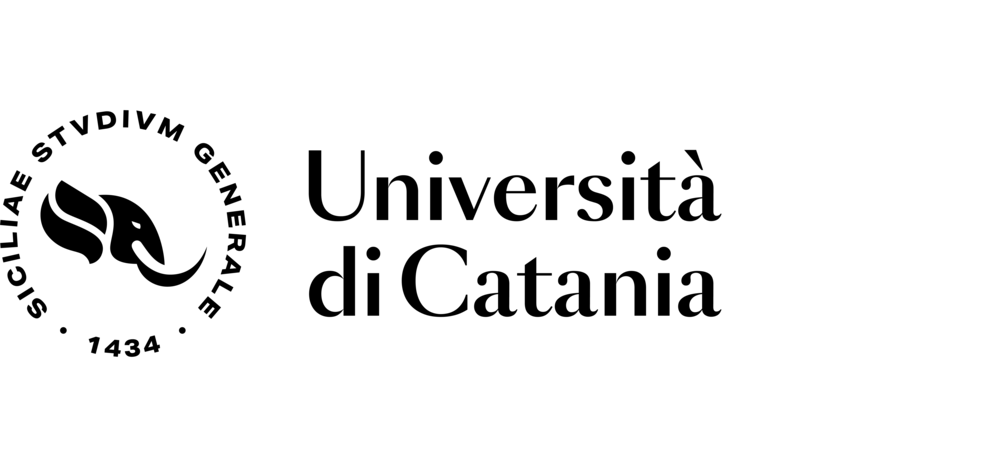
\includegraphics[width=0.8\textwidth]{image/loghi/Logo_UniCT.png}
\end{flushright}
\end{minipage}



    \begin{center}
        \vspace*{7cm}
            
        {\Huge
        \textbf{{Laboratorio di Fisica 3}}
        }
    
        \vspace{1cm}
        {\large
        {Appunti delle lezioni dell'A.A. 22/23}
        }
        \\
        \vspace{0.3cm}
        {\large
        {a cura di}
        }
        \\
        \vspace{0.3 cm}
        {\large
        {Virginia Marchetta}
        }
    \end{center}
\end{titlepage}
\frontmatter

\chapter*{Prefazione}
Quanto seguirà nelle prossime pagine sono gli appunti delle lezioni del corso di \textit{Laboratorio di Fisica 3} tenuto dalla professoressa Paola La Rocca. Le lezioni fanno riferimento all'anno accademico 2022/2023. La professoressa ha fornito il suo materiale. Se necessario ho integrato i discorsi tramite libri consigliati dal docente.


\hfill Virginia Marchetta

\chapter*{Programma del Corso}
\begin{itemize}
    \item[1] \textbf{Tecniche e strumenti di laboratorio}: Funzionamento e utilizzo di sensori per la misura di grandezze fisiche --- Sensori analogici e digitali --- Acquisizione dati da sensori --- Data logger --- Utilizzo di sistemi tradizionali e di microprocessori a basso costo --- Il sistema Arduino e sue applicazioni --- Multimetri digitali e oscilloscopi analogici e digitali --- Elementi base di tecnica del vuoto --- Attrezzature per la produzione del vuoto: principali tipi di pompe da vuoto --- Strumenti per la misura del vuoto --- Misura di radiazioni dall’infrarosso all’ultravioletto --- Fibre ottiche e trasporto della luce --- Spettrofotometri digitali --- Proprietà e utilizzo di sorgenti radioattive alfa, beta e gamma.
    
    \item[2] \textbf{Rivelatori di radiazione}: Interazione di particelle cariche pesanti con la materia – Relazione di Bethe-Bloch – Range – Straggling – Perdita di energia di elettroni e positroni – Radiazione di frenamento - Radiazione Cherenkov - Interazione dei fotoni con la materia – Effetto fotoelettrico, effetto Compton e produzione di coppie – Sciami elettromagnetici – Sviluppo longitudinale e trasversale di uno sciame elettromagnetico – I rivelatori di particelle nella fisica moderna - Classificazione dei rivelatori di particelle – Misura dell’energia, dell’impulso, della posizione, della massa e della carica delle particelle subatomiche – Proprietà generali di un rivelatore: sensibilità, risoluzione, efficienza, tempo morto - Rivelatori a gas – Camere a ionizzazione – Contatori Geiger – Rivelatori a semiconduttore – Rivelatori a strip, a drift e a pixel di silicio – Il danneggiamento da radiazione – Rivelatori a scintillazione - Scintillatori organici e inorganici – Risposta in luce – Fotomoltiplicatori – Guide di luce e fibre WLS – Fotodiodi a valanga e silicon photomultiplier.

    \item[3] \textbf{Elementi di elettronica}: Segnali impulsivi dai rivelatori – Segnali analogici e digitali – Standardizzazione dei segnali – Propagazione e trasporto dei segnali – Cavi coassiali e loro caratteristiche – Generatori di segnali - Alimentatori – Modulistica elettronica per la fisica nucleare – Lo standard NIM - Elementi base di elettronica lineare: preamplificatori, amplificatori, shaper – Elementi base di elettronica digitale – Combinazioni logiche di segnali: OR, AND, NOT – Convertitori analogico-digitale (ADC, QDC, TDC) – Discriminatori – Circuiti di coincidenza – Scale di conteggio - Sistemi di trigger – Cenni sui sistemi di acquisizione dati – Il software per l’acquisizione e la gestione dei dati.
    \item[4] \textbf{Analisi dei dati e tecniche di simulazione}: Richiami di statistica elementare - Indici per il valore centrale e indici di dispersione – Distribuzioni sperimentali – Distribuzione di Gauss – Distribuzione di Poisson – Errori sperimentali e loro trattamento - Test di significatività – Tecniche di analisi dati in fisica nucleare – Analisi di uno spettro a più componenti – Sottrazione del fondo – Fit non lineari – Uso di programmi di analisi dati multiparametrici - Simulazione di processi fisici – Tecniche Monte Carlo – Utilizzo del software ROOT per la simulazione e per l’analisi dei dati sperimentali - Cenno sui programmi di simulazione GEANT per i rivelatori di particelle.
\end{itemize}
\newpage
\tableofcontents
\newpage
\mainmatter

\chapter{Tecniche e strumenti di laboratorio}
\section{Misura di grandezze fisiche mediante sensori}
Il \textbf{sensore} è un trasduttore che si trova in diretta interazione con il sistema misurato. In ambito strettamente metrologico, il termine sensore è riferito solamente al componente che fisicamente effettua la trasformazione della grandezza d'ingresso in un segnale di altra natura. In base alla precedente descrizione un sensore può essere facilmente schematizzato come un blocco che riceve in ingresso la grandezza fisica non elettrica da misurare e fornisce in uscita la grandezza elettrica corrispondente:
\begin{center}
    
\includegraphics[width=8cm]{sensore.png}
\end{center}
Lo scopo di tale conversione di segnale è quello di interfacciare il mondo esterno con un sistema elettronico. I dispositivi in commercio spesso integrano al loro interno anche alimentatori stabilizzati, amplificatori di segnali, dispositivi di comunicazione remota, ecc. In quest'ultimo casi si preferisce definirli \textbf{trasduttori}. Bisogna tuttavia osservare che questa distinzione viene raramente seguita: nella maggior parte dei casi i due termini, sensore e trasduttore, vengono usati praticamente come sinonimi. E così faremo nel seguito di questa trattazione.\\
Un sensore viene detto \textbf{analogico} se la grandezza elettrica prodotta in uscita varia con continuità in risposta alla variazione della grandezza di ingresso. Viceversa un sensore viene detto \textbf{digitale} se i valori possibili in uscita sono limitati. Nel caso più semplice, quello dei cosiddetti \textit{sensori on-off}, i valori in uscita possono essere soltanto due.\\
La distinzione fra i due tipi di sensori, analogici e digitali, è importante in quanto le tecniche di trattamento del segnale prodotto dal sensore sono notevolmente diverse nei due casi. In parole semplici, il segnale prodotto da un sensore digitale può essere trattato direttamente da un circuito digitale: per esempio un dispositivo logico, un contatore oppure una scheda di acquisizione per computer. Viceversa i segnali prodotti dai sensori analogici devono essere trattati da circuiti analogici (filtri, circuiti di condizionamento, amplificatori). In seguito essi potranno eventualmente essere convertiti digitalmente (con convertitori analogici-digitali) e quindi trattati ulteriormente con elettronica di tipo digitale.\\
Oggigiorno esistono sensori in grado di misurare praticamente qualsiasi grandezza fisica. In base al tipo di grandezza misurata i sensori possono essere così classificati: meccanici, acustici, termici, magnetici, chimici,ecc... Vediamoli più nello specifico.
\section{Esempi di sensori analogici}
\begin{itemize}
    \item Sensore di forza;
    \item Sensore di pressione atmosferica;
    \item Sensore di intensità luminosa;
    \item Tanti altri: pH, carica elettrica, campo magnetico, accelerazione, umidità...
\end{itemize}
\section{Esempi di sensori digitali}
\begin{itemize}
    \item Sensore di posizione: in grado di rilevare la presenza di oggetti nelle immediate vicinanze. Il funzionamento è molto facile, il sensore emette un’onda di ultrasuoni ad una specifica frequenza verso l’eventuale target e aspetta il tempo necessario per l’eco di ritorno. Durante questo intervallo, misura la presenza e la distanza dell'ostacolo.
    \item Sensore a foto-traguardo: è costituito da una fotocellula ed un LED. 
    \item Sensore di moto rotatorio: è costituito da una puleggia ed un sistema digitale che converte l'angolo di rotazione in una grandezza misurabile.
\end{itemize}
Alcuni esempi di esperimenti con sensori:
\begin{itemize}
    \item Moto su un piano inclinato;
    \item Misura della velocità del suono;
    \item Studio dei battimenti;
    \item Urti elastici e anelastici;
    \item Oscillazioni non lineari e smorzate di un pendolo.
\end{itemize}

\section{Software di acquisizione dati}
Il software di acquisizione deve consentire:
\begin{itemize}
    \item Scelta dei sensori da utilizzare;
    \item Opzioni di campionamento e raccolta dati;
    \item  Modalità di visualizzazione dei risultati;
    \item Possibilità di salvare ed esportare i dati;
    \item Eventuali analisi grafiche e/o numeriche.
\end{itemize}
Software originale fornito dalla PASCO: \textit{Science Workshop}
\begin{itemize}
    \item Distribuzione libera;
    \item Utilizzabile sotto Windows (fino a XP).
\end{itemize}
Software più recenti della stessa Casa: Data Studio,...
\begin{itemize}
    \item Versioni utilizzabili anche con Windows 7, 10, Mac,...
    \item Versione di prova o «Light»,...
\end{itemize}








\chapter{Arduino Vecchio}
Arduino è una piattaforma hardware open-source capace di leggere un input, e tramite un set di istruzione è possibile creare progetti interattivi. Arduino si pone come lo strumento che permette una correlazione tra un microprocessore e il mondo esterno. \\
Tra le diverse schede sviluppate negli anni, la scheda utilizzata è l' \textit{Arduino uno board}. 

\begin{figure}[H]
    \centering
    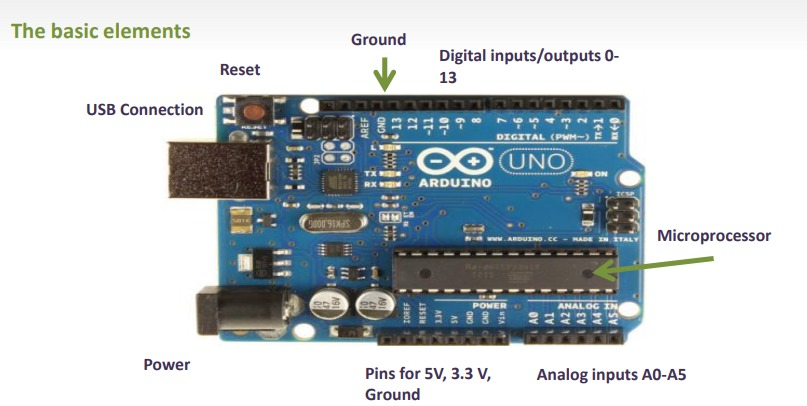
\includegraphics[scale=0.5]{Screenshot_20-3-2024_181852_.jpeg}
    \caption{Arduino uno}
    \label{fig:arduino_uno_vecchio}
\end{figure}
Tale schede è composta da 14 input/output pins digitali, 6 input pins analogici. La programmazione della scheda avviene tramite una porta USB, che permette la connessione con il PC, ove è istallato il software IDE: Integrated Development Enviroment, ovvero una paittaforma che permette la compilazione e il trasferimento del codice (sketch) alla scheda. \\
\newpage
\section{Linguaggio di programmazione}
Il linguaggio di Arduino è una sorta di C semplificato, per inizializzare uno sketch si fa uso della seguente struttura: \begin{center}
    Variable definition \\
void setup() \{ \\
// put your setup code here, to run once:\\
\}
void loop() \{\\
// put your main code here, to run repeatedly:\\
\}
\end{center}
Dove: \begin{itemize}
    \item setup: permette di inzializzare le variabili e i pin.
    \item loop: permette la run in maniera continua dello sketch, fin quanto la scheda è accesa, in tale struttura vengono inserite le istruzioni.
\end{itemize}
La sintassi di tale linguaggio è del tutto analoga al C, inoltre la definizione dei pin avviene attraverso la funzione \textbf{pinMode()} che definisce se un pin è input o output. \\
Si è gia accennato che gli input possono essere di due tipi: digitali e analogici. \\
Un input digitale può assumere solo 2 valori: \begin{itemize}
    \item 0 (0V) = LOW
    \item 1 (5V) = HIGH
\end{itemize}
è possibile fissare un valore ad un determinato Pin tramite la funzione \textbf{digitalWrite} e leggere tale valore tramite la funzione \textbf{digitalRead}. Arduino impiega 10 $\mu s$ per leggere un input digitale.  \\ \\
Un input analogico può assumere valori continui tra 0V e 5V, in maniera proporzionale alla grandezza fisica con cui ci si sta confrontando. A tali input sono associati dei sensori, chiamati: \textit{Sensori analogici}. Tali sensori devono essere collegati al \textbf{GROUND}. Alcuni tra questi sensori presentano 3 pin, in modo tale da essere collegati direttamente al \textbf{GROUND}, ai 5V e all'input analogico della scheda di arduino.\\

\section{Come posso leggere gli analog input?}
Il valore di tensione proporzionale alla grandezza fisica con cui ci si sta confrontando è trasformata in numeri compresi tra 0 e 1023 (ovvero 1024 possibili valori). \\
Tale processo è effettuato tramite l'utilizzo di un particolare circuito elettrico: \textbf{ADC} (Analog to Digital Converter), che si trova direttamente sulla scheda Arduino. \\
I valori sono proprio 1024 in quanto dipendono dalla risoluzione dell' ADC, dettata dal numero di bits (10 per arduino, e dunque $2^{10}=1024$). \\
La variazione minima di tensione che possiamo apprezzare è dettata dal numero di valori che possono essere assunti, appunto nel caso di Arduino:
\begin{equation}
    \Delta V_{min} = \frac{5 V}{2^{10}}= 4.88 mV
\end{equation}
Inoltre Arduino impiega 100 $\mu s$ per leggere un input analogico.

\section{Sketch di Arduino}
Le attività sono proposte dalla docente. 

\chapter{Sistemi di controllo}

Nella vita di tutti i giorni, ognuno di noi compie delle azioni che gli permettono di interfacciarsi e dialogare con il mondo esterno: dallo svegliarsi e prepararsi un caffè, fino a guidare l'auto per andare al lavoro.
Tutte queste azioni vedono noi come i protagonisti che gestiscono cosa fare e quando farlo a seconda delle condizioni che l'ambiente ci propone.

Portiamo alcuni esempi di azioni quotidiane. Consideriamo un automobilista che sta guidando e arriva davanti a un incrocio regolato da un semaforo. Supponiamo che quest'ultimo sia rosso: allora l'automobilista inizierà a frenare fino ad arrestarsi. Questo accade perché l'automobilista, guardando il colore rosso del semaforo, associa a questo colore il significato di arresto/stop, e quindi durante la marcia, inizierà a premere il pedale del freno fino a quando non si fermerà. Dopodiché, passato qualche secondo, il semaforo torna a essere verde. In tal caso, l'automobilista assocerà il colore verde al significato di via libera/partenza e quindi inizierà a premere il pedale dell'acceleratore per poter partire.\footnote{Ovviamente dopo aver inserito la marcia.} \\
Immaginiamo ora un altro esempio. Supponiamo di star lavando i piatti: oltre prendere il sapone, apriremo l'acqua calda che si troverà ad una certa temperatura. Allora, per non scottarci gireremo il rubinetto verso l'acqua fredda. Continueremo quindi a muovere il rubinetto finché non troviamo la giusta temperatura dell'acqua per lavare i piatti e per non scottarci. 

Questi esempi visti sono la visualizzazione di come un \textit{Sistema di Controllo} funziona.

\begin{figure}[H]
  \centering
  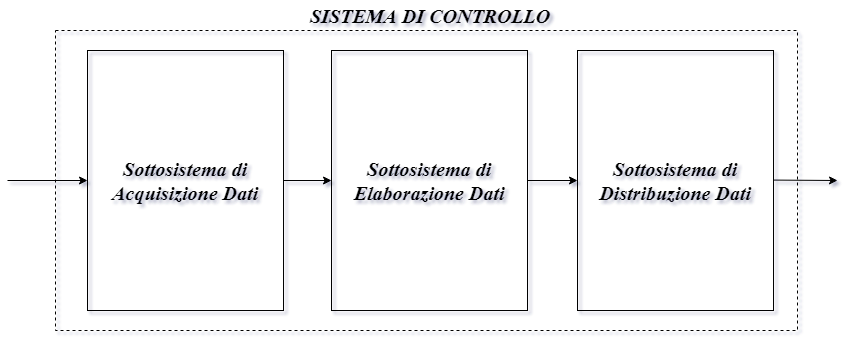
\includegraphics[scale=0.4]{image/foto_sistemi_di_controllo/Sistemi_di_Controllo.png}
  \caption{Sistema di Controllo}\label{fig:sistema_di_controllo}
\end{figure}

Un sistema di controllo \cref{fig:sistema_di_controllo} è un sistema che presenta dei componenti, o generalmente dei sottosistemi\footnote{Come abbiamo visto anche noi possiamo essere considerati un sistema di controllo}, capaci di interagire tra loro in modo tale da controllare, manipolare, regolare delle informazioni provenienti dal mondo esterno. In particolare:

Il Sottosistema di Acquisizione Dati ha il compito di:
\begin{itemize}[leftmargin=1.2cm, itemsep=1pt, topsep=5pt]
  \item  Acquisire, prelevare, misurare le informazioni che provengono dal mondo esterno attraverso i sensori;
  \item Convertire tali informazioni in una forma più maneggevole per il Sottosistema di Elaborazione;
  \item Inviare i dati misurati al Sottosistema di Elaborazione.
\end{itemize}

Il Sottosistema di Elaborazione Dati ha il compito di:
\begin{itemize}[leftmargin=1.2cm, itemsep=1pt, topsep=5pt]
  \item  Ricevere i dati che il sottosistema di Acquisizione gli ha fornito;
  \item Elaborare queste informazioni mediante\footnote{Come vedremo più avanti stiamo parlando di circuiti elettrici ed elettronici che sono molto utili per gestire e manipolare le informazioni. Negli esempi precedenti il sistema di elaborazione è il cervello umano.}:
        \begin{itemize}[itemsep=1pt, topsep=2pt]
          \item Circuiti logici --- Sequenziali (Flip-Flop, Shift Register, Contatori)\footnote{Sono dei componenti base della logica sequenziale.} o Combinatori (And, Or, Not);
          \item Circuiti analogici --- Amplificatori Operazionali (Invertente, Non invertente, Sommatori, Differenziali, Esponenziali, Logaritmici)\footnote{Si tratta di amplificatori operazionali in configurazioni differenti. Ognuno di questi ha un nome che ci permette di capire come verrà manipolato il segnale analogico}.
        \end{itemize}
  \item Inviare i dati opportunamente elaborati al Sottosistema di Distribuzione
\end{itemize}

Il sottosistema di Distribuzione Dati ha il compito di:
\begin{itemize}[leftmargin=1.2cm, itemsep=1pt, topsep=5pt]
  \item Captare le informazioni che gli vengono dati dal Sottosistema di Elaborazione;
  \item Convertire i dati in una forma richiesta dagli attuatori;
  \item Attraverso gli attuatori, fornire al mondo esterno le informazioni in una maniera a noi comprensibile.
\end{itemize}

Un circuito elettronico, o più in generale un sistema, senza sottosistema di acquisizione o distribuzione dati sarebbe inutile perché esso non potrà mai dialogare con il mondo esterno. Se, invece, non presenta un sottosistema di elaborazione, esso non potrà mai gestire le informazioni che gli vengono fornite e le informazioni che dovrà distribuire.

Prima di passare alla descrizione di ogni sottosistema dobbiamo introdurre alcune definizioni.

  \section{Le grandezze fisiche}

  In fisica, una \textbf{\textit{grandezza fisica}} è una proprietà oggettiva di un corpo o di un fenomeno che può essere quantificata, ovvero espressa tramite un numero e un'unità di misura. Il requisito fondamentale affinché una proprietà sia considerata una grandezza fisica è la sua misurabilità. L'operazione di misura consiste nel confrontare la grandezza in esame con un'altra della stessa natura, scelta come campione di riferimento (l'unità di misura), per determinare quante volte quest'ultima è contenuta nella prima.

  Queste grandezze possiamo distinguerle a loro volta in:

  \begin{table}[H]
    \centering
    \begin{tabular}[t]{@{} p{0.45\textwidth} p{0.45\textwidth} @{}}
      % Riga dei titoli centrati
      \multicolumn{1}{c}{\textbf{\textit{Grandezze Fisiche Elettriche}}} & \multicolumn{1}{c}{\textbf{\textit{Grandezze Fisiche non Elettriche}}} \\[1em]
      
      % Colonna di sinistra
      \vspace{0pt}
      \textbf{\textit{Facilmente Manipolabili}}
      \begin{itemize}[leftmargin=*, nosep]
        \item Tensione
        \item Corrente
      \end{itemize}
      
      \vspace{1em} % Spazio verticale tra i due blocchi a sinistra
      
      \textbf{\textit{Difficilmente Manipolabili}}
      \begin{itemize}[leftmargin=*, nosep]
        \item Resistenza
        \item Capacità
        \item Induttanza
        \item Ecc.
      \end{itemize}
      &
      % Colonna di destra
      \vspace{0pt}
      \begin{itemize}[leftmargin=*, nosep]
        \item Temperatura
        \item Posizione
        \item Luminosità
        \item Forza
        \item Peso
        \item Pressione
        \item Suono
        \item Volume
        \item Ecc.
      \end{itemize}
    \end{tabular}
  \end{table}

  Una Grandezza Elettrica si dice Facilmente Manipolabile quando può essere manipolata mediante semplici circuiti, come ad esempio quelli di cui parlavamo prima nel sottosistema di elaborazione dati, mentre una Grandezza Elettrica si dice Difficilmente Manipolabile quando per essere manipolata necessita di circuiti piuttosto complessi.

  Ci concentreremo principalmente sullo schema di un Sottosistema di Acquisizione Dati e sulle varie tipologie di Sensori.

  \section{Sottosistema di Acquisizione Dati}

  Un Sottosistema di Acquisizione ad un Solo Canale utilizza un solo sensore o trasduttore per ricevere informazioni dal mondo esterno. Nel caso in cui avessimo più di un sensore o trasduttore parleremmo di un Sottosistema di Acquisizione Multicanale.

  Lo schema generale di un Sottosistema di Acquisizione ad un solo canale è il seguente:

  \begin{figure}[H]
    \centering
    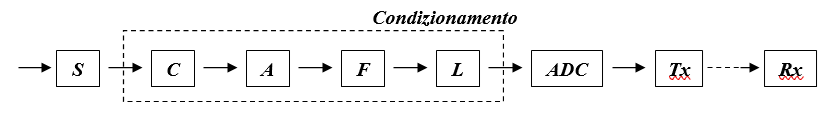
\includegraphics[scale=0.5]{image/foto_sistemi_di_controllo/Sottosistema_di_acqusizione_un_canale.png}
    \caption{Sottosistema di Acquisizione ad un solo canale}\label{fig:sottosistema_di_acquisizione_un_canale}
  \end{figure}

	Andiamo a descrivere singolarmente i vari blocchi:
  \begin{itemize}[leftmargin=1.2cm, itemsep=1pt, topsep=5pt]
    \item \textbf{\textit{(S)} Sensore o Trasduttore}: \\
          Il sensore è un dispositivo che riceve una grandezza fisica non elettrica dal mondo esterno e la converte in una grandezza elettrica. \textbf{\textit{È sempre presente in un Sottosistema di Acquisizione, in particolare ce n’è uno per ogni canale di acquisizione.}}
    \item \textbf{\textit{(C)} Convertitore}: \\
          Il convertitore è un circuito che converte una grandezza in un’altra a noi più utile. Ce ne sono tantissimi, qui di seguito ne mostriamo alcuni esempi:
          \begin{itemize}[itemsep=1pt, topsep=2pt]
            \item ($R \rightarrow V$) Convertitore Resistenza -- Tensione: In questo caso si tratta di un circuito che converte una grandezza difficile da manipolare come la resistenza in una grandezza facile da manipolare come la tensione.
            \item ($I \rightarrow V$) Convertitore Corrente – Tensione: Se il sensore produce come segnale una corrente mentre il Sistema di Elaborazione vuole il segnale sotto forma di tensione allora è necessario un convertitore di questo tipo.
          \end{itemize}
          \textbf{\textit{Si usa tutte le volte in cui per un qualche motivo vogliamo convertire una grandezza in un’altra. Se necessario, è possibile utilizzarne più di uno.}}
    \item \textbf{\textit{(A)} Amplificatore e \textit{(T)} Traslatore}\\
      L’\textbf{Amplificatore} è un circuito in grado di amplificare, cioè moltiplicare per una costante l’ampiezza della grandezza elettrica presente al suo ingresso.
      \textbf{\textit{Viene utilizzato per portare l’ampiezza del segnale al valore richiesto dal Sottosistema di Elaborazione Dati.}} 

      Il \textbf{Traslatore} è un circuito in grado di sommare un valore costante (positivo o negativo) al segnale spostando la forma d’onda verticalmente della quantità desiderata. \textbf{\textit{Viene in genere utilizzato per azzerare l’offset}}

      Mediante un Amplificatore Sommatore è possibile Traslare ed Amplificare il segnale con un unico circuito.

      \begin{figure}[H]
        \centering
        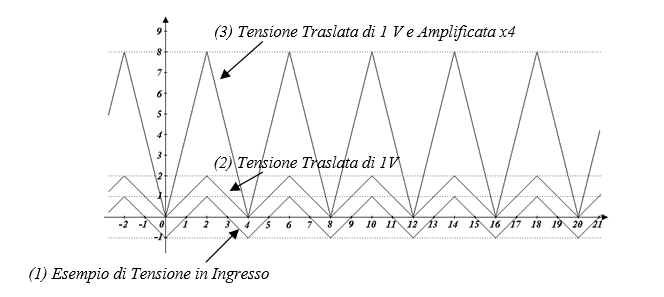
\includegraphics[scale=0.6]{image/foto_sistemi_di_controllo/Amplificatore_traslatore.png}
        \caption{Segnale traslato e amplificato}\label{fig:amplificatore_traslatore}
      \end{figure}

    \item \textbf{\textit{(F)} Filtro}: \\
          Il filtro è un circuito selettivo in frequenza, esso lascia passare inalterate alcune frequenze mentre ne blocca altre.
          Viene utilizzato principalmente per:
          \begin{itemize}[itemsep=1pt, topsep=2pt]
            \item Eliminare o ridurre il rumore che viaggia sovrapposto all’informazione;
            \item Eliminare parti del segnale.
          \end{itemize}
    \item \textbf{\textit{(L)} Linearizzatore}: \\
          Qualora il sensore abbia una caratteristica I/O non lineare potrebbe essere necessario un circuito in grado di rendere lineare tale caratteristica. Esso prende il nome di linearizzatore.
          \begin{figure}[H]
            \centering
            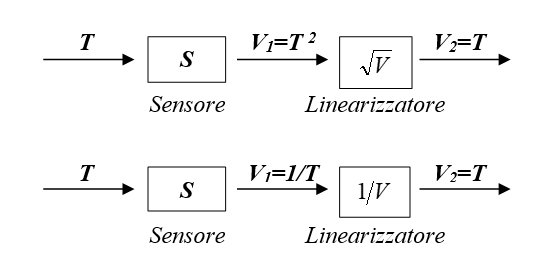
\includegraphics[scale=0.5]{image/foto_sistemi_di_controllo/linearizzatore.png}
            \caption{Esempi di linearizzatori}\label{fig:linearizzatore}
          \end{figure}
    \item \textbf{Condizionamento} \\
          Con condizionamento si intende l'insieme dei blocchi che convertono il segnale prodotto dal sensore (o dal trasduttore) nella forma richiesta dal Sottosistema di Elaborazione dati. Include al suo interno i blocchi Convertitore. Amplificatore e Traslatore, Filtro e Linearizzatore.
          
    \item \textbf{Convertitore Analogico Digitale \textit{(ADC)}}\\
          Il convertitore analogico digitale è un circuito elettronico capace di convertire una grandezza elettrica analogica (cioè che può assumere qualsiasi valore all'interno di un certo intervallo) in una digitale (cioè che può assumere due soli valori ai quali associamo i simboli '0' e '1').
          
          Si utilizza quando il Sottosistema di Elaborazione Dati accetta solo segnali di tipo digitali (Es. Computer, Arduino).
    \item \textbf{Convertitore Digitale Analogico \textit{(DAC)}}\\
          Il convertitore digitale analogico è un circuito elettronico capace di convertire una grandezza elettrica digitale in una analogica.

          Si utilizza quando il segnale prodotto dal sensore è di tipo di digitale e il Sottosistema di Elaborazione Dati accetta segnali di tipo analogico, anche se viene utilizzato di rado (Es. Amplificatori Operazionali).
    \item \textbf{\textit{(Tx)} Trasmettitore e \textit{(Rx)} Ricevitore}\\
          Un trasmettitore è un dispositivo capace di trasmettere a distanza (mediante cavo, luce o radiofrequenza) un segnale analogico o digitale.\\
          Un ricevitore è un dispositivo capace di ricevere a distanza (mediante cavo, luce o radiofrequenza) un segnale analogico o digitale.
  \end{itemize}

  Questa è la struttura generale di come un Sottosistema di Acquisizione dati funziona.  

  \section{Sensori ed Attuatori}

  Da quanto detto finora si potrebbe pensare che i Sensori ed i Trasduttori siano la stessa cosa, ma non è così.

  \begin{itemize}
    \item \textbf{\textit{Definizione di Sensore}}\\
          Un sensore è un dispositivo che, \textbf{senza il bisogno di alimentazione esterna}, è in grado di convertire una Grandezza Fisica non Elettrica in una Grandezza Elettrica.
          \begin{figure}[H]
            \centering
            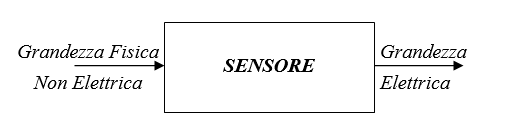
\includegraphics[scale=0.6]{image/foto_sistemi_di_controllo/sensore.png}
            \caption{Sensore}\label{fig:sensore}
          \end{figure}
    \item \textbf{\textit{Definizione di Convertitore}}\\
          Qualora il sensore dia in uscita una Grandezza Elettrica Difficile da Manipolare è possibile collegare ad esso un circuito in grado di convertire tale grandezza in una Semplice da Manipolare. \\
	        Poiché si tratta di un circuito elettronico vero e proprio, \textbf{esso ha bisogno di essere alimentato mediante un generatore esterno.}
          \begin{figure}[H]
            \centering
            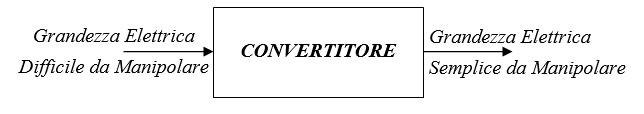
\includegraphics[scale=0.6]{image/foto_sistemi_di_controllo/convertitore.png}
            \caption{Convertitore}\label{fig:convertitore}
          \end{figure}
    \item \textbf{\textit{Definizione di Trasduttore}}\\
          Collegando in cascata (uno dopo l’altro) un Sensore ed un Convertitore si ottiene un Trasduttore, cioè un dispositivo che, alimentato mediante un generatore esterno, è in grado di convertire una Grandezza Fisica non Elettrica in una Grandezza Fisica Elettrica Facile da Manipolare.
          \begin{figure}[H]
            \centering
            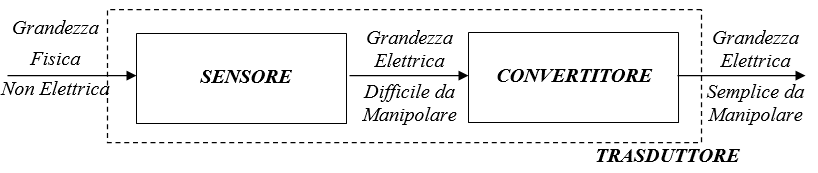
\includegraphics[scale=0.55]{image/foto_sistemi_di_controllo/trasduttore.png}
            \caption{Trasduttore}\label{fig:trasduttore}
          \end{figure}
  \end{itemize}

  All'interno del Sottosistema di Distribuzione Dati\footnote{Che non tratteremo.} troviamo altri dispositivi altrettanto importanti: gli attuatori. Di seguito è possibile vedere uno schema di confronto tra sensore (o trasduttore) e l'attuatore:
  
  \begin{figure}[H]
    \centering
    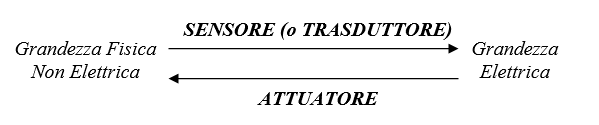
\includegraphics[scale=0.6]{image/foto_sistemi_di_controllo/sensore_attuatore.png}
    \caption{Sensore e Attuatore}\label{fig:sensore_attuatore}
  \end{figure}

  Un \textbf{\textit{attuatore}} è un dispositivo che converte una Grandezza Elettrica in un Grandezza Fisica non Elettrica. Ad esempio: motore, led, elettrocalamita, altoparlante, display, etc.

  \begin{figure}[H]
    \centering
    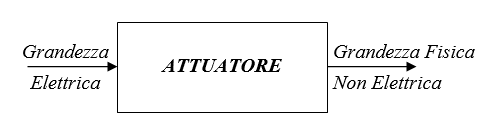
\includegraphics[scale=0.6]{image/foto_sistemi_di_controllo/attuatore.png}
    \caption{Attuatore}\label{fig:attuatore}
  \end{figure}

  Queste definizioni sono molto importanti perché ci permettono di capire come funziona e come poter realizzare un sistema di controllo. In fisica, che sia teorica o sperimentale, ci sarà sempre bisogno di utilizzare un sistema di controllo, dai software di simulazione alla realizzazione di un circuito vero e proprio per l'acquisizione dei dati.

    \section{Microprocessori e Microcontrollori}
    % Differenza tra microprocessore (CPU di un PC) e microcontrollore (un intero computer su un singolo chip, ottimizzato per interagire con l'esterno).

    Le informazioni provenienti dal sottosistema di acquisizione dati devono essere elaborate, manipolate e trasformate da un sottosistema di elaborazione dati.

    Nei dispositivi moderni questo è possibile grazie all'utilizzo di microprocessori e microcontrollori.  

        \section{Microprocessore}

        Un \textbf{\textit{microprocessore}}, e in generale un \textit{processore}, è un dispositivo hardware in grado di gestire dati sulla base di istruzioni che gli vengono fornite. La sua struttura varia moltissimo, andando da semplici elaboratori di segnale fino alla CPU \textit{(Central Processing Unit)} all'interno di un computer. 

        Di seguito la struttura di una CPU:

        \begin{figure}[H]
            \centering
            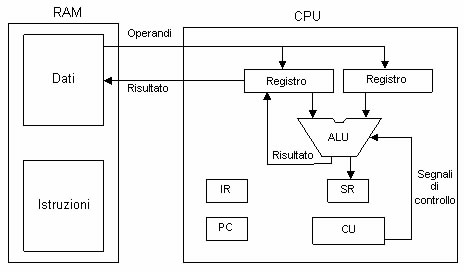
\includegraphics[scale=0.57]{image/foto_sistemi_di_controllo/cpu_schema.jpg}
            \caption{Schema di una CPU}\label{fig:cpu_schema}
        \end{figure}

        Tra i vari blocchi, i più importanti sono:
        \begin{itemize}
            \item \textbf{Unità di Controllo} (control unit o CU): è il cuore centrale di una CPU. Preleva istruzioni e dati dalla memoria centrale, decodifica le istruzioni e le invia ad un'unità aritmetico-logica per poi eseguirle. La Cu ha anche il compito di organizzare il lavoro delle altre unità di elaborazione.
            \item \textbf{Unità aritmetico-logica} (Arithmetic Logic Unit o ALU): si occupa di eseguire le operazioni logiche ed aritmetiche. Si tratta della unità che svolge i calcoli.
            \item \textbf{Clock}: anche se non riportato nell'immagine, il clock è quel segnale che scandisce e sincronizza tutte le operazioni che avvengono all'interno della CPU. Solitamente si tratta di un segnale logico (onda quadra) con frequenze elevatissime, dell'ordine dei GHz. Senza il clock perderemmo la sincronizzazione e ciò porterebbe a degli errori che possono essere di calcolo o di comunicazione tra i vari blocchi.
            \item \textbf{Registri}: i registri sono delle memorie che hanno un tempo di accesso nettamente inferiore a quello della memoria centrale, cioè sono più veloci. Senza di essi, le varie operazioni che la CU deve eseguire sarebbero lentissime. In tal caso avere frequenze di clock così elevate sarebbe del tutto inutile perché la CU dovrebbe attendere il tempo necessario di accedere alla memoria centrale.
        \end{itemize}

        \section{Microcontrollore}

        Un \textbf{\textit{microcontrollore}} (MicroController Unit o MCU), è un dispositivo integrato\footnote{Un circuito integrato (in inglese integrated circuit, abbreviato IC) è un circuito elettronico miniaturizzato dove i vari transistor sono stati formati tutti nello stesso istante grazie a un unico processo fisico-chimico.} su singolo circuito elettronico. Utilizza tecniche di microelettronica per ridurre in un piccolo pacchetto (o package) vari componenti quali CPU (Central Processing Unit), memoria e diversi pin di ingresso e uscita, attraverso i quali è possibile interagire con il mondo esterno.

        Nato come evoluzione alternativa al microprocessore è utilizzato generalmente in sistemi embedded ovvero per applicazioni specifiche di controllo digitale (special purpose) non riprogrammabili dall'utente per altri scopi, spesso con una piattaforma hardware dedicate.

        \begin{figure}[H]
            \centering
            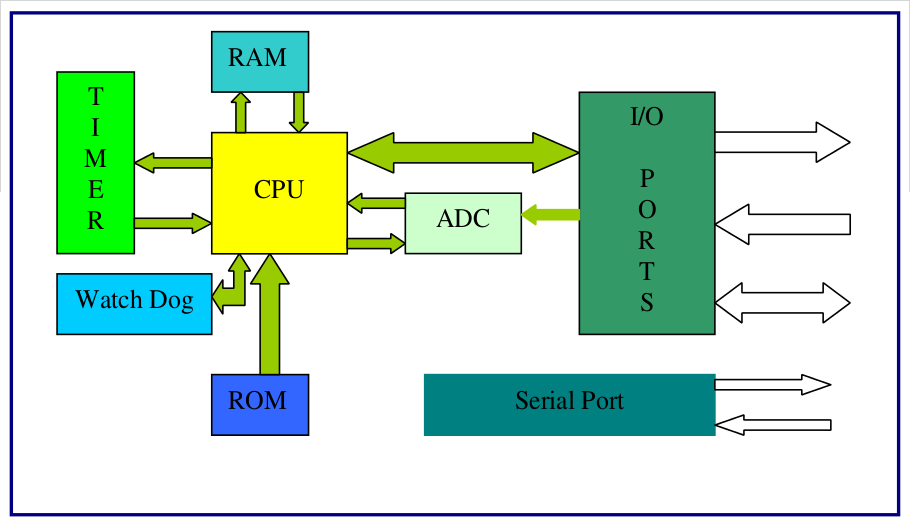
\includegraphics[scale=0.25]{image/foto_sistemi_di_controllo/microcontrollore_schema.png}
            \caption{Schema di un microcontrollore}\label{fig:microcontrollore_schema}
        \end{figure}

        Alcuni esempi di sistemi embedded in cui vengono usati i microcontrollori sono: controllo di hard disk e di stampanti, calcolatrici, sistemi di allarme, etc.\\
        Si può pensare a un microcontrollore come un piccolo computer, in cui è possibile collegare sensori e attuatori per svolgere un determinato compito (task).

\chapter{Arduino}

Arduino è un sistema di sviluppo hardware e software che permette la creazione di sistemi di controllo utilizzando delle schede elettroniche dotate di microcontrollore su circuito stampato.

\begin{figure}[H]
  \centering
  
\includegraphics[scale=0.2]{image/loghi/png-transparent-arduino-hd-logo.png} \quad 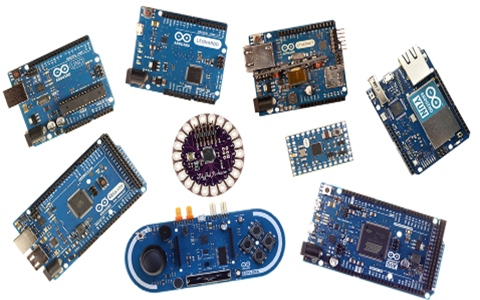
\includegraphics[scale=0.4]{image/foto_arduino/tipi_di_schede.png}
  \caption{Logo Arduino e varie schede}\label{fig:logo_arduino}
\end{figure}

L'idea nacque nel 2005 da alcuni membri dell'Interaction Design Institute di Ivrea come strumento per la prototipazione rapida e per scopi hobbistici, didattici e professionali. Il nome della scheda deriva da quello del bar di Ivrea frequentato dai fondatori del progetto, nome che richiama a sua volta quello di Arduino d'Ivrea, Re d'Italia nel 1002.

Le schede elettroniche, chiamate board, sono formate da varie parti e componenti che consentono il collegamento con unità esterne, sia digitali che analogiche. Il collegamento può avvenire mediante l’utilizzo dei pin di input e output (I/O) digitali o analogici. Di fatto stiamo parlando di un sottosistema di elaborazione a cui colleghiamo con i pin di ingresso tutti quei componenti che fanno parte del sottosistema di acquisizione dati e con i pin di uscita tutti quei componenti che fanno parte del sottosistema di distribuzione dati.
    
Esistono varie tipologie di schede, ognuna con un nome differente. Ad esempio, possiamo nominare le board Arduino Uno \cref{fig:logo_arduino}, Arduino Mini, Arduino Nano, Arduino Leonardo, etc., ognuna delle quali viene scelta a seconda dell'utilizzo che si intende effettuare. Infatti, ogni board presenta un numero differente di pin di I/O, una diversa alimentazione e anche componenti che permettono di utilizzare protocolli di comunicazione più complessi come ad esempio il WiFi o il Bluetooth.

Grazie alla sua interfaccia utente semplice e intuitiva, Arduino è stato utilizzato in migliaia di progetti e applicazioni diverse. Il software Arduino è facile da usare per i principianti, ma al contempo sufficientemente flessibile per gli utenti più esperti. Funziona su Mac, Windows e Linux. Insegnanti e studenti lo utilizzano per costruire strumenti scientifici a basso costo, per dimostrare principi di chimica e fisica o per avvicinarsi alla programmazione e alla robotica. Designer e architetti realizzano prototipi interattivi, musicisti e artisti lo usano per installazioni e per sperimentare nuovi strumenti musicali. 

  \section{Interfaccia software di Arduino}

  Il controllo della scheda avviene utilizzando l'IDE (Integrated Development Environment), cioè l'ambiente di sviluppo del codice di Arduino. Una volta installato dal sito ufficiale, al suo interno è possibile scrivere un programma in un linguaggio simile al C++ e che, una volta compilato, viene caricato sulla scheda tramite un collegamento USB.
  
  \begin{figure}[H]
    \centering
    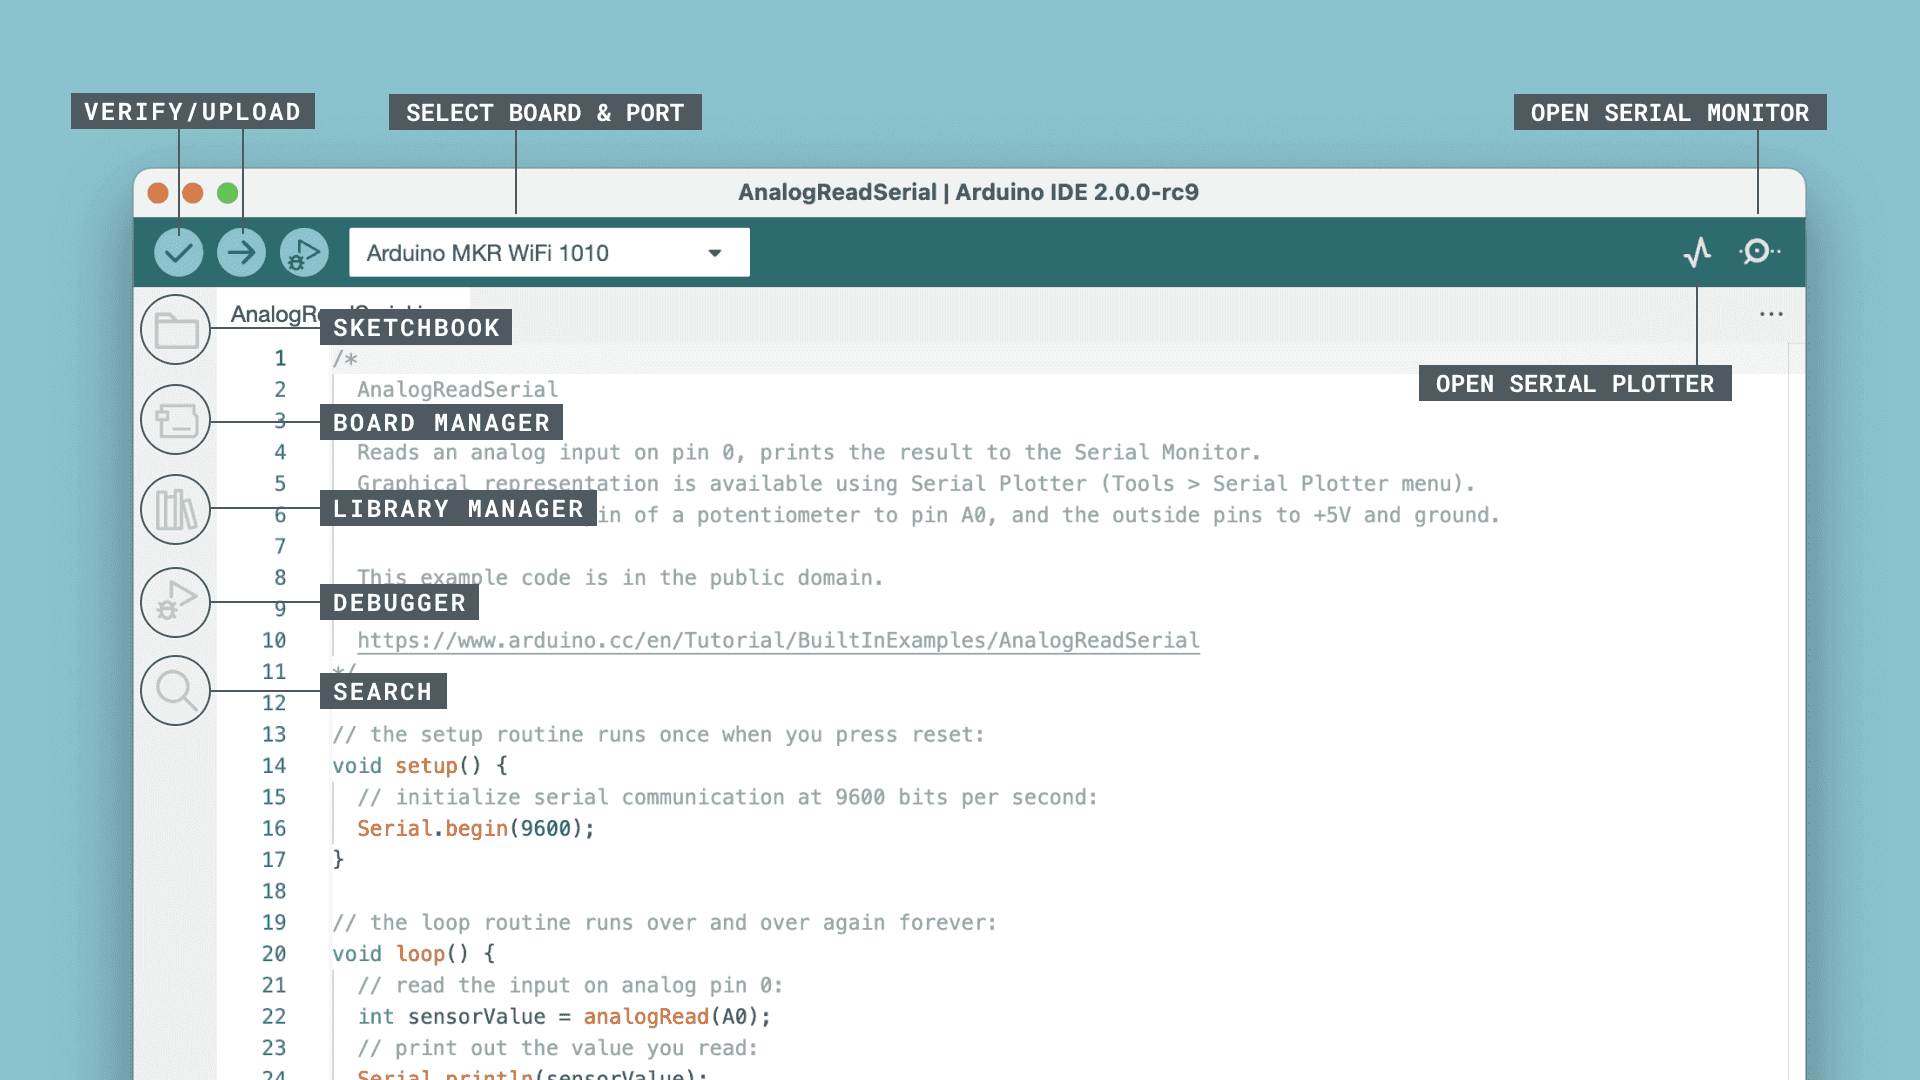
\includegraphics[scale=0.2]{image/foto_arduino/ide_arduino.png}
    \caption{IDE di Arduino}\label{fig:ide_arduino}
  \end{figure}

  Come si vede in \cref{fig:ide_arduino} l'IDE è suddivisa in diverse sezioni:

  \begin{itemize}[leftmargin=1.2cm, itemsep=1pt, topsep=5pt]
    \item \textit{la barra superiore degli strumenti}. Partendo da sinistra troviamo:
          \begin{itemize}[leftmargin=0.5cm, itemsep=1pt, topsep=3pt]
            \item il pulsante di \textit{compilazione} per compilare il codice e vedere se sono presenti errori;
            \item il pulsante di \textit{caricamento} per caricare il codice sulla board;
            \item il pulsante di \textit{debug} per avviare una sessione di debug interattiva, che permette di analizzare il comportamento del codice in tempo reale e trovare errori.
            \item uno \textit{slider} che ci permette di selezionare la scheda collegata tramite USB;
            \item il \textit{serial plotter} ovvero un grafico che in tempo reale permette di rappresentare una grandezza proveniente da una variabile all'interno del codice;
            \item il \textit{serial monitor} che permette di inviare e ricevere dati alla board attraverso la comunicazione USB.
          \end{itemize}
    \item \textit{la barra laterale}. Partendo dall'alto troviamo:
          \begin{itemize} [leftmargin=1.2cm, itemsep=1pt, topsep=5pt]
            \item lo \textit{sketchbook} ovvero la cartella principale dove vengono salvati i progetti (chiamati "sketch") e le relative librerie;
            \item il \textit{gestore delle schede} che serve a installare, aggiornare o rimuovere il supporto per le diverse schede microcontrollore ;
            \item il \textit{gestore librerie} che serve a ricercare, installare, aggiornare e gestire facilmente le librerie di terze parti e quelle ufficiali;
            \item gli ultimi due sono il pulsante di debug e il pulsante di ricerca.
          \end{itemize}
    \item \textit{l'editor di testo}: la parte più importante dove all'interno viene scritto il vero e proprio codice che ci permetterà di gestire variabili, sensori ed attuatori mediante alcune funzioni. Una volta salvato lo skecth quest'ultimo sarà un file con estensione ".ino". L'editor dell'ambiente di sviluppo,  oltre alle solite funzioni presenti in tutti editor, ha delle caratteristiche particolari che facilitano la scrittura dei programmi, in particolare:
          \begin{itemize}[leftmargin=1.2cm, itemsep=1pt, topsep=5pt]
            \item il syntax highlighting, cioè la capacità di evidenziare il testo con colori diversi in base alle regole del linguaggio di programmazione utilizzato;
            \item l'auto-indentazione: l'editor provvede ad indentare correttamente il codice mentre lo si digita (ad esempio aumentando di due spazi il rientro del blocco di codice di una funzione).
          \end{itemize}
  \end{itemize}

    \subsection{Il linguaggio di programmazione}

    Il linguaggio di programmazione usato in Arduino si basa su C/C++ ed è integrato da un framework chiamato Wiring, progettato per semplificare la creazione di prototipi elettronici con funzioni per gestire in maniera semplice le interfacce di input/output della scheda.
    
    I programmi sono scritti al PC utilizzando il software Arduino vengono trasmessi mediante la porta seriale USB al microcontrollore ATmega 328P e memorizzati nella memoria EEPROM\footnote{La EEPROM (Electrically Erasable Programmable Read-Only Memory) è un tipo di memoria non volatile, cancellabile e riprogrammabile elettricamente, utilizzata in elettronica per memorizzare piccole quantità di dati che devono persistere anche senza alimentazione. È molto comune nei microcontrollori e centraline auto} del microcontrollore ATmega 328P. Il programma viene eseguito successivamente in modo ciclico. Il codice sorgente di un programma per Arduino si chiama sketch. La struttura di base di un programma (sketch) scritto per la scheda Arduino è molto semplice e può essere suddiviso in tre parti:

    \begin{itemize}[leftmargin=1.2cm, itemsep=1pt, topsep=5pt]
      \item la prima parte, posta generalmente all’inizio dello sketch per una migliore leggibilità, contiene l’inserimento degli eventuali file di libreria e la dichiarazione di tutte le variabili che verranno utilizzate. Le variabile poste in questa sezione sono variabili globali.
      \item  la seconda parte, costituita dalla funzione \lstinline[style=myArduino]{void setup()} utilizzata per configurare la scheda, per esempio per programmare i pin digitali in ingresso o uscita. Queste istruzioni vengono eseguite solo una volta.
      \item la terza parte, costituita dalla funzione \lstinline[style=myArduino]{void loop()} che contiene il programma da eseguire ciclicamente. 
    \end{itemize}

    Entrambe le funzioni sono necessarie per l’esecuzione del programma. Il contenuto scritto dentro le parentesi graffe della funzione setup, contiene la dichiarazione delle variabili, viene eseguita una sola volta e serve per programmare i pin del Microcontrollore ATmega 328P utilizzando la funzione pinMode, o per inizializzare la comunicazione seriale. 
    La funzione loop include il codice da eseguire in modo continuo: lettura ingressi, attivazione uscite, ecc.

    Alcuni delle funzioni più utilizzate sono:
    \begin{itemize}[leftmargin=1.2cm, itemsep=1pt, topsep=5pt]
      \item \lstinline[style=myArduino]{pinMode(pin, INPUT/OPUTPUT)};
      \item \lstinline[style=myArduino]{digitalRead(pin)};
      \item \lstinline[style=myArduino]{digitalWrite(pin, HIGH/LOW)};
      \item \lstinline[style=myArduino]{analogRead(pin)};
      \item \lstinline[style=myArduino]{analogWrite(pin, valore)};
      \item \lstinline[style=myArduino]{delay(tempo)};
    \end{itemize}


  \section{Arduino Uno}
    
    Arduino UNO è la scheda ideale per iniziare con l'elettronica e la programmazione ed è una delle schede più robuste con cui si può iniziare. UNO è la scheda più utilizzata e documentata dell'intera famiglia Arduino.


    \begin{figure}[H]
    \centering
    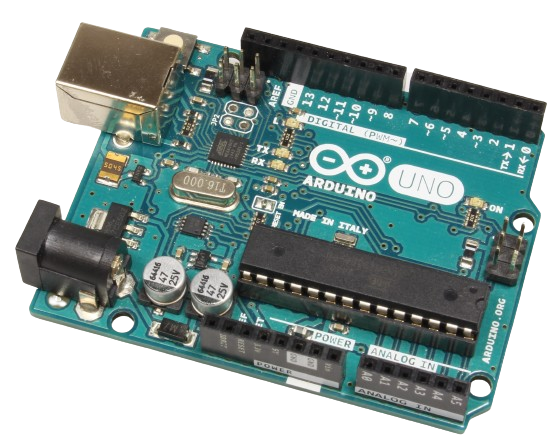
\includegraphics[scale=0.2]{image/foto_arduino/Arduino_uno_r3_isometr-removebg-preview.png}
    \caption{Scheda Arduino Uno}\label{fig:arduino_uno}
    \end{figure}

    Arduino UNO è una scheda a microcontrollore basata sull'ATmega328P prodotto da Atmel. Presenta queste caratteristiche:

    \begin{itemize}[leftmargin=1.2cm, itemsep=1pt, topsep=5pt]
      \item 14 pin di input/output digitali (di cui 6 utilizzabili come uscite PWM);
      \item 6 ingressi analogici;
      \item un risonatore ceramico da 16 MHz (Clock);
      \item connessione porta USB;
      \item un connettore di alimentazione jack;
      \item un connettore ICSP\footnote{L'ICSP (In-Circuit Serial Programming) su Arduino è un metodo per programmare il microcontrollore direttamente sulla scheda (o su breadboard) senza rimuoverlo, utilizzando il protocollo SPI. È essenziale per "masterizzare" (caricare) il bootloader, ripristinare schede bloccate o programmare chip vergini.};
      \item un pulsante per il reset.
    \end{itemize}

    Tale scheda contiene tutto il necessario per il funzionamento del microcontrollore; è sufficiente collegarla a un computer tramite un cavo USB o alimentarla con un adattatore CA/CC o una batteria per iniziare.

    \begin{figure}[H]
    \centering
    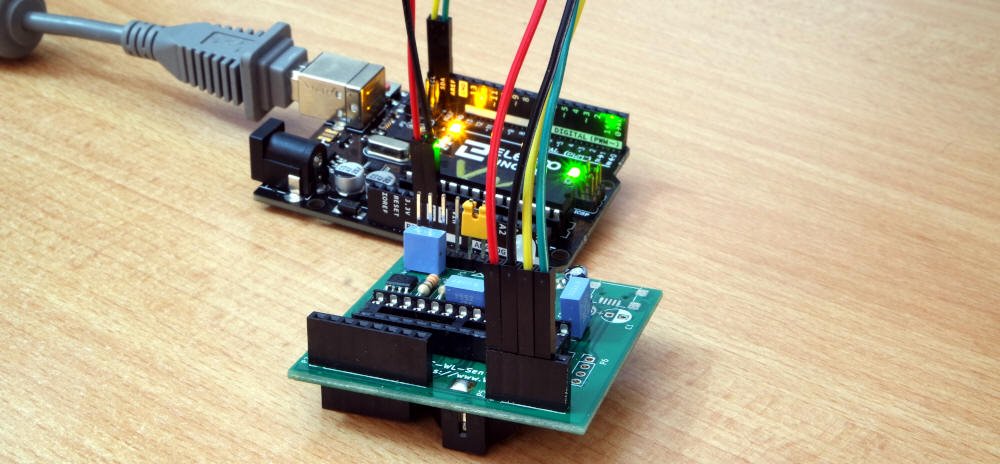
\includegraphics[scale=0.3]{image/foto_arduino/arduino_uno_esempio.jpg}
    \caption{Esempio di utilizzo di Arduino Uno}\label{fig:arduino_uno_esempio}
    \end{figure}

    Ci sarebbe da riportare ulteriori caratteristiche tecniche ma non lo faremo perché esula dai nostri interessi.

    \subsection{I Pin di Arduino}

    In generale, i pin sono quei componenti di un circuito che permettono il collegamento con altri dispositivi; in questo caso i pin sono dei fori che si trovano direttamente sulla scheda con cui possiamo collegare altre boards, sensori ed attuatori mediante dei cavetti.

    I cavetti forniti solitamente in dotazione con Arduino possono essere di tipo maschio-maschio, maschio-femmina oppure femmina-femmina. Combinandoli opportunamente si ottengono collegamenti più lunghi, utili per connettere dispositivi più lontani all'interno del circuito.

    \begin{figure}[H]
        \centering
        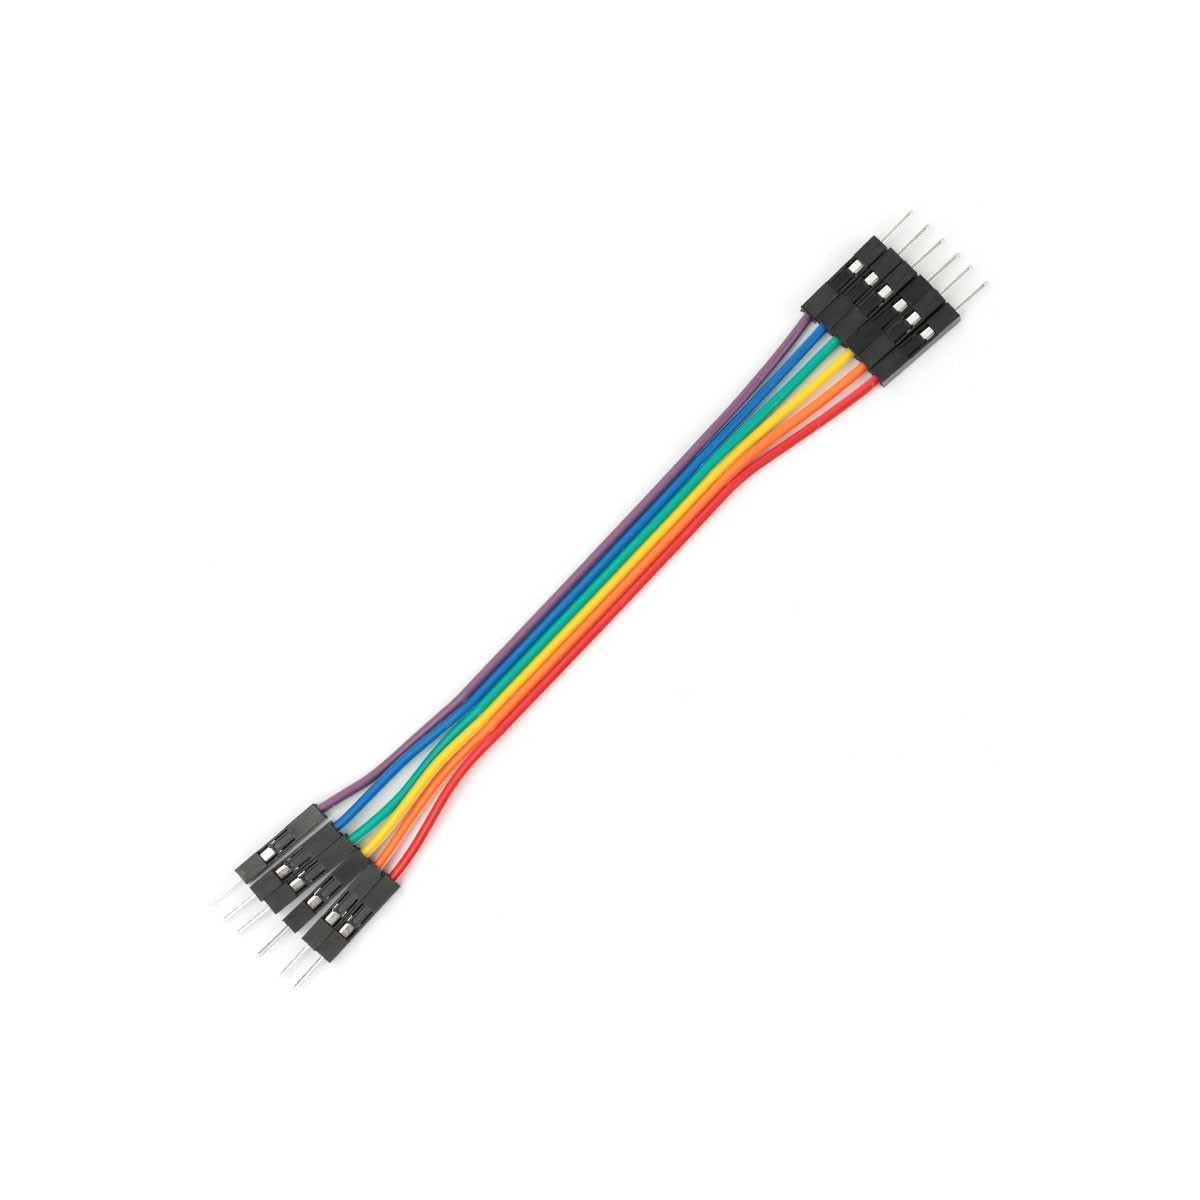
\includegraphics[scale=0.11]{image/foto_arduino/cavo_maschio_maschio.jpg} \quad 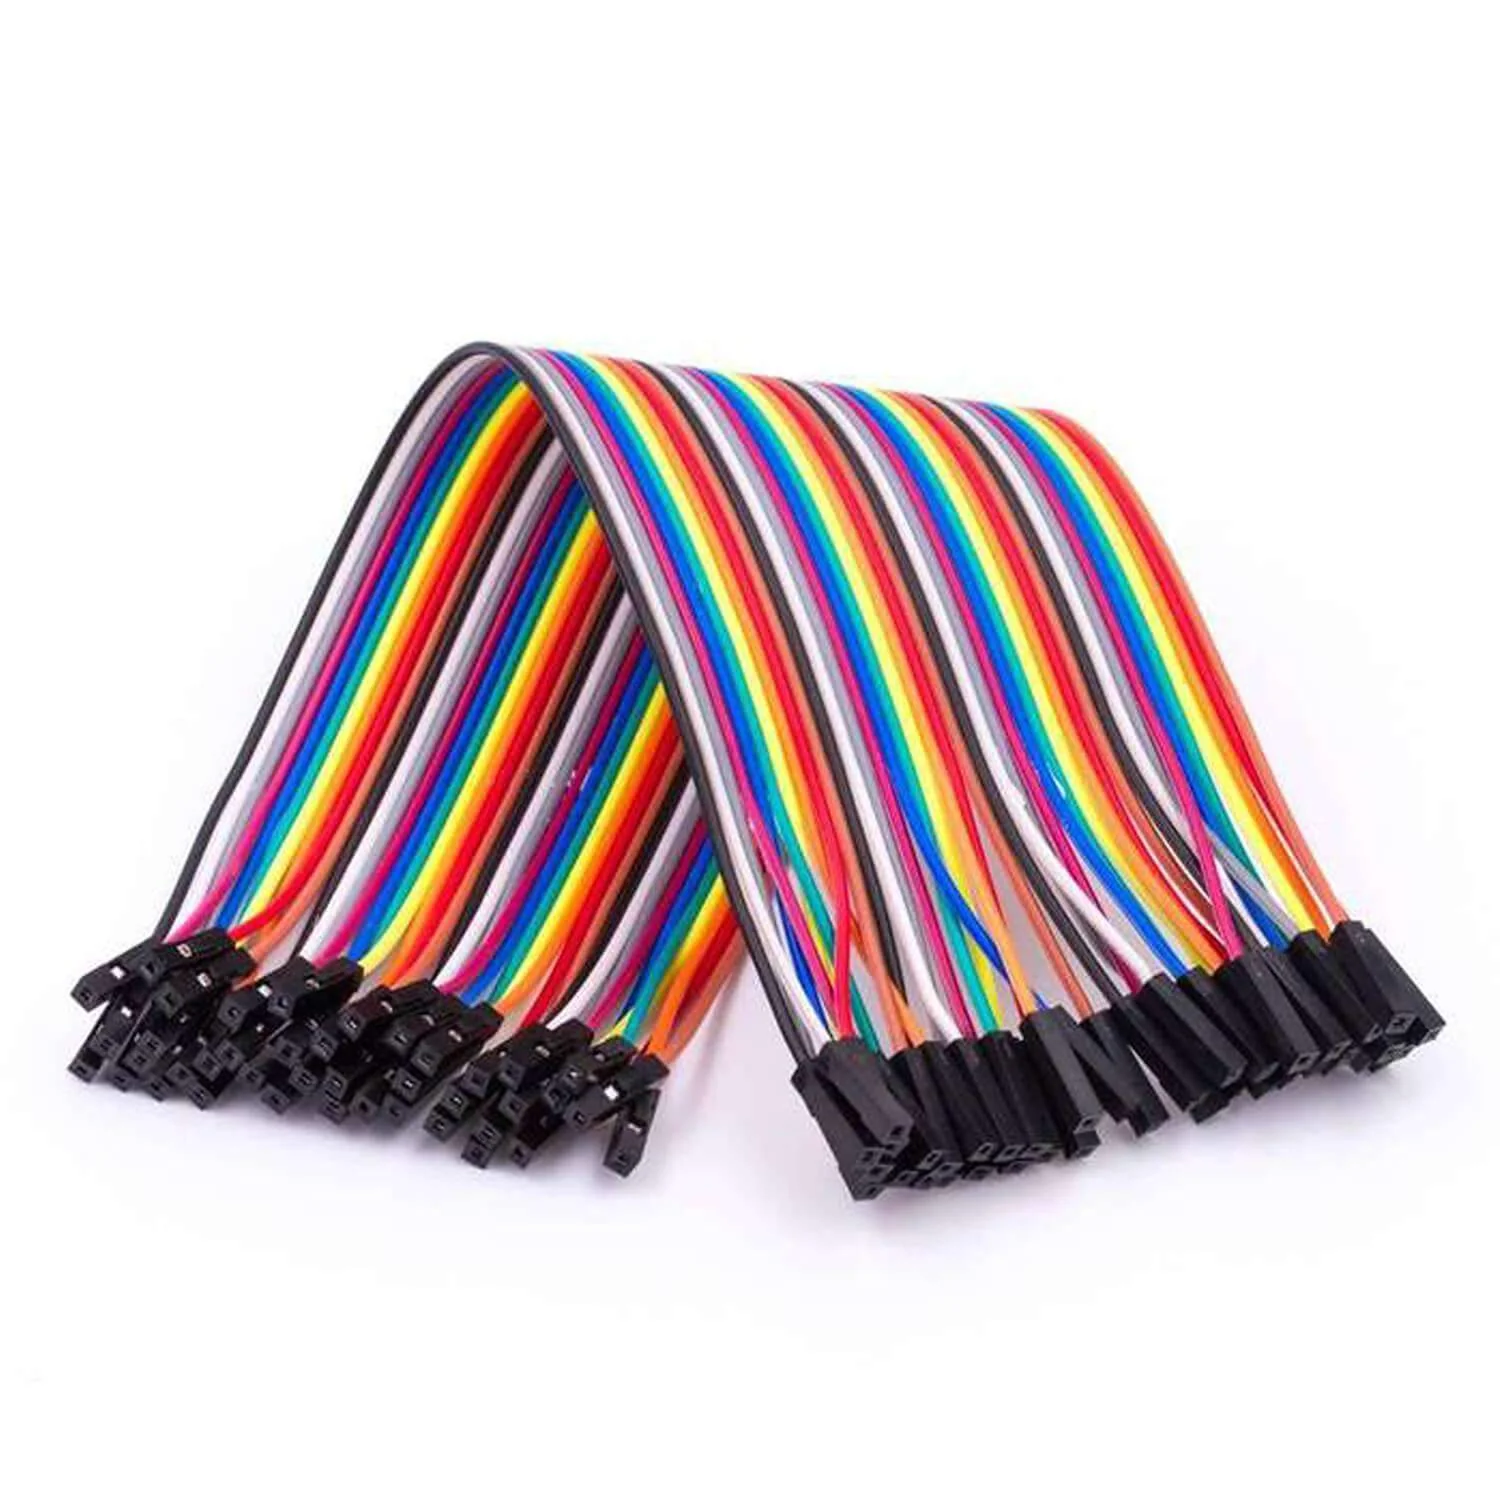
\includegraphics[scale=0.07]{image/foto_arduino/cavo_femmina_femmina.png} \quad 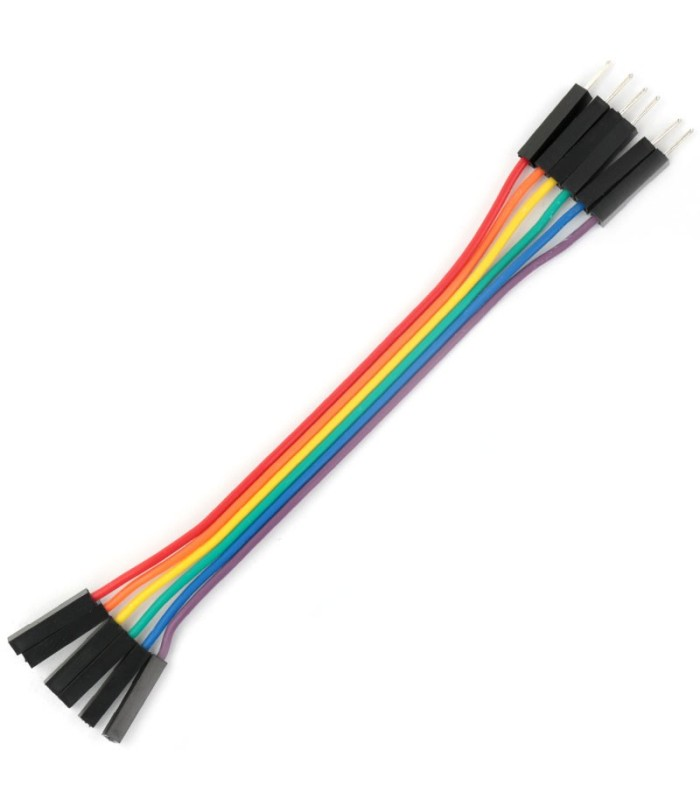
\includegraphics[scale=0.14]{image/foto_arduino/cavo_maschio_femmina.jpg}
        \caption{Connettori}\label{fig:cavetti}
    \end{figure}

    Impostare i pin di Arduino come ingresso o uscita digitale è molto semplice: all'interno della funzione \lstinline[style=myArduino]{void setup()} basta inserire \lstinline[style=myArduino]{pinMode(pin, INPUT)} nel caso in cui volessimo usare il pin come ingresso digitale o \lstinline[style=myArduino]{pinMode(pin, OUTPUT)} nel caso in cui volessimo usare il pin come uscita digitale. Di default i pin digitali sono impostati come ingressi, quindi non è necessario dichiararli esplicitamente con \lstinline[style=myArduino]{pinMode()}: farlo, però, è buona abitudine così da non confondersi con altri pin della scheda durante la stesura del codice.

    I pin di ingresso richiedono una corrente estremamente bassa al circuito con cui sono collegati. Infatti, quest'ultimo vede il pin come un resistore equivalente di $100 M\Omega$ e ciò significa che è necessaria pochissima corrente per far commutare il pin di ingresso da uno stato all'altro. Se all'interno del codice il pin viene configurato lo stesso con \lstinline[style=myArduino]{pinMode(pin, INPUT)} e se non viene collegato nulla, o se i fili collegati non sono connessi ad altri circuiti, vi saranno dei cambiamenti repentini e casuali dello stato del pin a causa del rumore elettrico dall'ambiente circostante.

    \begin{figure}[H]
        \centering
        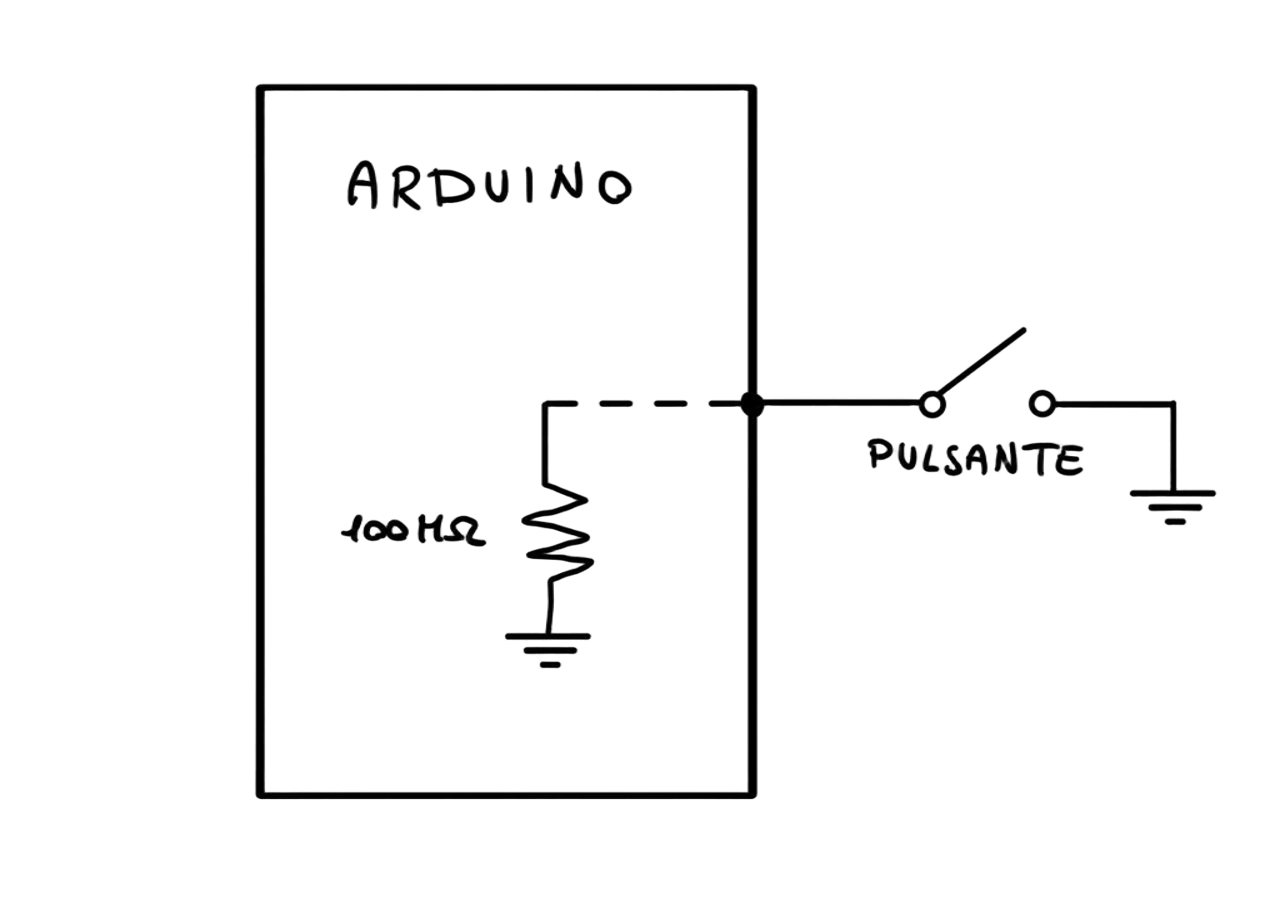
\includegraphics[scale=0.18]{image/foto_arduino/alta_impedenza.png}
        \caption{Alta impedenza Arduino}\label{fig:alta_impedenza}
    \end{figure}

    Vediamo adesso alcuni esempi per poter utilizzare i pin di Arduino come uscite digitali o ingressi digitali.

    %Esempio collegamento pin di uscita (led)

    Immaginiamo ora di voler collegare un pulsante o un interruttore ad un pin di Arduino. Sappiamo già che di default quest'ultimo è impostato come un ingresso digitale e quindi non ci sarà il bisogno di inserire all'interno del codice la funzione \lstinline[style=myArduino]{pinMode()}. \\
    Colleghiamo quindi un'estremità (o terminale) del pulsante al pin di Arduino e l'altro al GND. Dentro il \lstinline[style=myArduino]{void loop()} ci sarà la parte di programma che accenderà un led quando premiamo il pulsante e che lo spegnerà quando non lo premiamo.

    Sembrebbe essere molto semplice: quando il pin di ingresso legge uno stato logico basso accende il led, quando legge uno stato logico alto lo spegne. Ebbene, in questo ragionamento che abbiamo fatto c'è un problema. Quando premiamo il pulsante tutto funziona correttamente: essendo collegato al GND si porta ad uno stato logico basso e il led viene acceso. Invece, quando non lo premiamo lo stato del pulsante non è determinato, proprio perché l'ingresso di Arduino è un ingresso ad alta impedenza. Il led potrebbe quindi o accendersi o spegnersi o addirittura lampeggiare proprio perché lo stato del pin di ingresso viene influenzato dal rumore esterno.

    Per evitare situazioni del genere, spesso è utile indirizzare un pin di ingresso ad uno stato noto. Tale operazione può essere fatta aggiungendo al pin di ingresso una resistenza di PULL-UP o di PULL-DOWN.

    \begin{figure}[H]
        \centering
        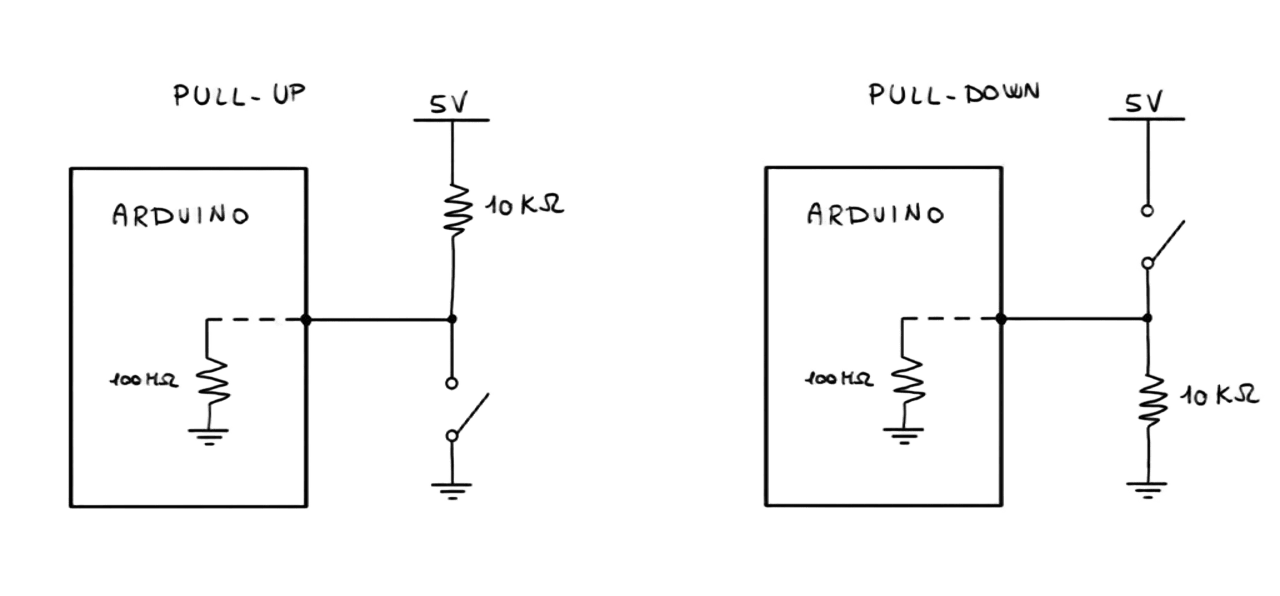
\includegraphics[scale=0.23]{image/foto_arduino/pull_up_down.png}
        \caption{Resistenza di pull-up e pull-down}\label{fig:pull_up_pull_down}
    \end{figure}

    Prova di modifica


\chapter{Sorgenti di Radiazione}
Le sorgenti radioattive forniscono un mezzo conveniente per testare e calibrare i rivelatori e sono strumenti essenziali sia nel laboratorio di fisica nucleare che in quello delle alte energie. Una comprensione dei processi nucleari di base nelle sorgenti radioattive è quindi una necessità prima di iniziare a lavorare in laboratorio\footnote{Per una discussione più dettagliata rimandiamo il lettore a uno qualsiasi dei testi standard di fisica nucleare per maggiori informazioni.}.\\
In generale, con \textbf{radiazione} si indica generalmente il trasporto di energia nello spazio senza movimento di corpi macroscopici e senza il supporto di mezzi materiali.\\
Esse di distinguono principalmente in \textit{non ionizzanti} e \textit{ionizzanti}. Quest’ultime, diversamente dalle prime, sono radiazioni dotate di elevato contenuto energetico, in grado di rompere i legami atomici del corpo urtato e caricare elettricamente atomi e molecole neutri ionizzandoli. Le sorgenti di radiazione possono essere sia naturali che artificiali; le prime sono quelle a cui siamo soggetti tutti i giorni ed esse non sono nocive, mentre le seconde sono pericolose e dannose per l'organismo, alcuni esempi di sorgenti artificiali sono gli acceleratori di particelle.\\
Esistono diverse tipologie di radiazioni:
\begin{itemize}
    \item Radiazioni cariche: causate da particelle cariche pesanti (protoni, particelle $\alpha$, ioni pesanti) e da elettroni;
    \item Radiazioni neutre: causate da neutroni e radiazioni elettromagnetiche (raggi $\gamma$, raggi X);
    \item Radiazione cosmica secondaria (muoni, elettroni).
\end{itemize} 
L'intervallo di energia di interesse abbraccia oltre sei ordini di grandezza, da circa $10$ eV a $10$ MeV. Mentre la radiazione cosmica secondaria a un range energetico dei GeV.\\
Le radiazioni di interesse differiscono anche per la loro capacità di penetrazione. Le radiazioni "morbide", come le particelle alfa o i raggi X a bassa energia, penetrano solo piccoli spessori di materiale, dell'ordine di alcuni cm di aria e di circa $100$ $\mu$m per materiali solidi. Le particelle beta sono generalmente più penetranti e possono attraversare spessori di circa qualche millimetro.  Le radiazioni "più dure", come i raggi gamma o i neutroni, sono molto più penetranti, possono attraversare spessori possono di dimensione dei millimetri o centimetri senza compromettere seriamente le proprietà della radiazione. I muoni cosmici sono i più penetranti, possono attraversare anche spessori di parecchi metri di materiali solidi. Comunque è importante dire che tutto dipende dall'energia della radiazione.


\section{Stabilità dei nuclei}
I nuclei si possono classificare in \textit{nuclei stabili} e \textit{nuclei instabili}. Un nucleo è stabile quando il numero dei protoni e dei neutroni non cambia nel tempo. Viceversa, i nuclei instabili si trasformano continuamente, fino a raggiungere una nuova condizione di stabilità che non necessariamente appartiene allo stesso elemento chimico.
L'instabilità dell'atomo è una causa della radioattività o decadimento radioattivo perché durante il processo di trasformazione il nucleo instabile emette verso l'esterno delle particelle di diversa natura per raggiungere un livello di stabilità maggiore.

\section{Carta di Segrè}
I nuclei stabili si trovano soltanto lungo una stretta fascia del piano Z-N (nota anche come carta deinuclidi o di Segrè), tutti gli altri nuclei sono instabili. Nel grafico di seguito è riportato nell'asse delle ascisse i valori di $Z$, dove Z è il numero di protoni, e nell'asse delle ordinate  $N=A-Z$, dove $A$ è il numero di massa e $N$ il numero di
neutroni.
\begin{center}
    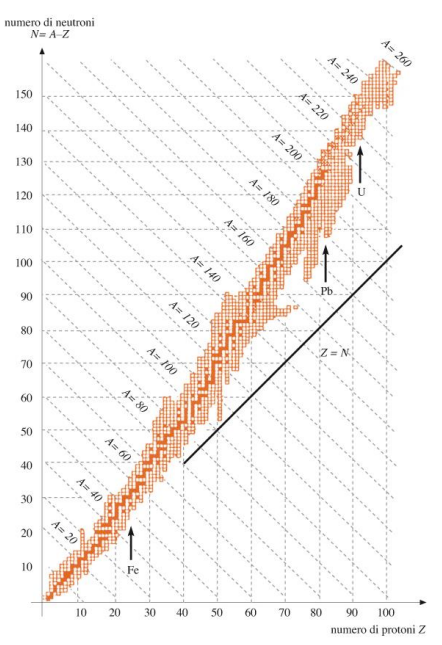
\includegraphics[width=8cm]{nuclei_stabili.png}
\end{center}
\begin{itemize}
    \item $1<Z<20$: i nuclei sono stabili quando il numero di protoni è uguale al numero di neutroni;
    \item $Z>20$: i nuclei sono stabili quando il numero di neutroni è maggiore al numero di protoni, questo perchè il numero maggiore di neutroni serve a ridurre l'effetto repulsivo coulumbiano tra i protoni, se no si avrebbe la disintegrazione del nucleo dovuto all'allontanamento dei protoni.
    \item $Z=82$: è l'ultimo elemento con nucleo stabile; esso è il piombo-82;
    \item $Z>84$: i nuclei sono sempre instabili e radioattivi.
\end{itemize}

\section{Legge del decadimento radioattivo}
Il momento esatto in cui un atomo instabile decadrà in un altro nucleo (che può essere sia instabile sia stabile)è ritenuto casuale e impredicibile. Ciò che si può fare, dato un campione di un particolare isotopo, è notare che il numero di decadimenti rispetta una precisa legge statistica. L'attività, cioè il numero di decadimenti che ci si aspetta avvenga in un intervallo dt, è proporzionale al numero N di atomi (o nuclei) presenti.
Sia $N(t)$ un elevato numero di nuclei radioattivi (radionuclidi) di una data sostanza al tempo $t$, la variazione del numero $N(t)$ di nuclei nell'intervallo $dt$ è data da
$$dN=-\lambda N(t)dt$$
dove  $\lambda$  è detta \textit{costante di decadimento}; è caratteristica della sostanza in questione e rappresenta il numero medio di decadimenti del singolo nucleo nell'unità di tempo. Il segno meno sta ad indicare che la popolazione radioattiva diminuisce col passare del tempo; integrando l’equazione precedente si ricava l’espressione del numero di nuclei presenti ad un generico istante $t$ successivo a quello iniziale
$$N(t)=N_0 e^{-\lambda t}$$
che rappresenta un \textit{decadimento esponenziale}. 
\begin{center}
    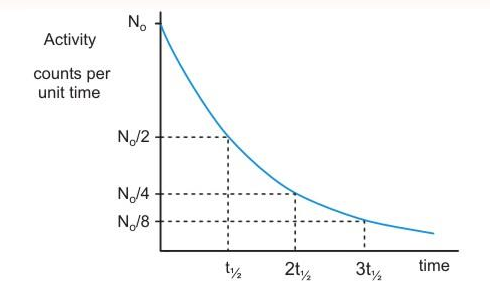
\includegraphics[width=8cm]{cost_dec_1.png}
\end{center}
Bisogna notare che questa rappresenta solamente una soluzione approssimata, in primo luogo perché rappresenta una funzione continua, mentre l'evento fisico reale assume valori discreti, poiché descrive un processo casuale, solo statisticamente vero. Comunque, poiché nella gran parte dei casi $N$ è estremamente grande, la funzione fornisce un'ottima approssimazione\\
La pendenza della curva dipende dal valore di $\lambda$, più è grande $\lambda$ più la curva è ripida, invece per valori piccoli la curva è meno ripida.
\begin{center}
    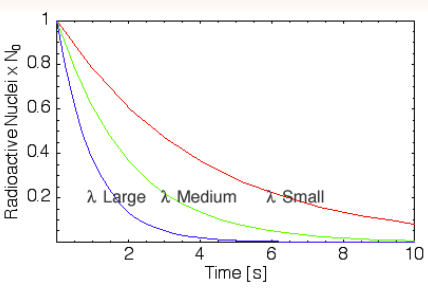
\includegraphics[width=8cm]{cost_dec_2.png}
\end{center}
Spesso capita che un nucleo possa essere soggetto a vari tipi di decadimento; in questo caso la probabilità totale di decadimento sarà la somma delle probabilità dei singoli modi di decadimento ciascuno caratterizzato da una costante per unità di tempo.\\
Si definisce \textit{attività} di una sorgente radioattiva il prodotto
$$A(t)=\lambda N(t)= \lambda N_0 e^{-\lambda t}$$
Essa rappresenta il numero di nuclei radioattivi che decadono nell'unità di tempo nell'intorno dell'istante $t$. L'unità di misura è il \textit{bequerel} (Bq) ed è pari ad 1 decadimento al secondo $1~~ Bq=1~~s^{-1}$. Una più vecchia unità di misura dell'attività è il \textit{curie} associata all'attività di 1g di radio; è stato fissato che $1~~Ci=3.7*10^{10}~~Bq=3.7*10^{10}~~s^{-1}$.\\
Oltre alla costante di decadimento $\lambda$ il decadimento radioattivo è caratterizzato da un'altra costante chiamata \textit{vita media}. Ogni atomo vive per un tempo preciso prima di decadere e la vita media rappresenta appunto la media aritmetica sui tempi di vita di tutti gli atomi della stessa specie. Può essere definito come il tempo necessario dopo il quale il numero di radionuclidi iniziali si è ridotto di un fattore $\frac{1}{e}$. La vita media viene rappresentata dal simbolo $\tau$,essa è legato a $\lambda$ dalla relazione:
$$\tau=\frac{1}{\lambda} $$
Un altro parametro molto usato per descrivere un decadimento radioattivo è dato dal \textit{tempo di dimezzamento} $t_\frac{1}{2}$. Dato un campione di un particolare radionuclide, il tempo di dimezzamento ci dice dopo quanto tempo saranno decaduti un numero di atomi pari alla metà del totale ed è legato alla vita media e alla costante di decadimento dalle relazioni:
$$t_\frac{1}{2}=\frac{\ln{2}}{\lambda} ~~ t_{\frac{1}{2}}=\tau\ln 2$$
Molte delle sostanze radioattive presenti in natura sono ormai decadute, e quindi non sono più presenti in natura, ma possono essere prodotte solo artificialmente. Per avere un'idea degli ordini di grandezza in gioco, si può dire che la vita media dei vari radionuclidi può variare da $10^9$ anni fino a $10^{-12}$ secondi.\\
L'insieme degli elementi ottenuti per decadimenti successivi costituisce una \textit{famiglia radioattiva}. In natura esistono tre famiglie radioattive principali: la famiglia dell'uranio, quella dell'attinio e quella del torio.\\
Storicamente i decadimenti nucleari sono stati raggruppati in tre classi principali: decadimento beta, decadimento alfa e decadimento gamma. A questa prima classificazione si sono aggiunte l'emissione di neutroni, l'emissione di protoni e la fissione spontanea. Mentre il decadimento alfa e il decadimento beta cambiano il numero di protoni nel nucleo (cambiando così la natura chimica del nucleo stesso), il decadimento gamma avviene fra stati dello stesso nucleo e comporta solo la perdita di energia. Andiamo ad analizzarli più nel dettaglio.

\section{\texorpdfstring{Decadimento $\beta$}{Decadimento beta}}
Un decadimento $\beta$ è un decadimento che coinvolge la trasformazione di un protone in un neutrone (con emissione di un neutrino ed un elettrone positivo, detto positrone) 
$$p\longrightarrow n+ e^+ +\nu$$
$$(A,Z)\longrightarrow (A,Z-1)$$
oppure la trasformazione di un neutrone in un protone (con emissione di un neutrino ed un elettrone)
$$n\longrightarrow p+ e^- +\overline{\nu}$$
$$(A,Z)\longrightarrow (A,Z+1)$$
Ovviamente variando il numero di protoni, cambiano le proprietà chimiche dell'elemento, cioè si ha la trasformazione di un elemento in un altro (il numero A rimane invariato, Z può aumentare o diminuire di una unità).
Il decadimento $\beta$ è un \textit{decadimento a tre corpi} (nucleo residuo, neutrino, elettrone o positrone) in cui lo spettro è continuo anziché essere discreto come nel caso di un decadimento $\alpha$ a due corpi.
\begin{center}
  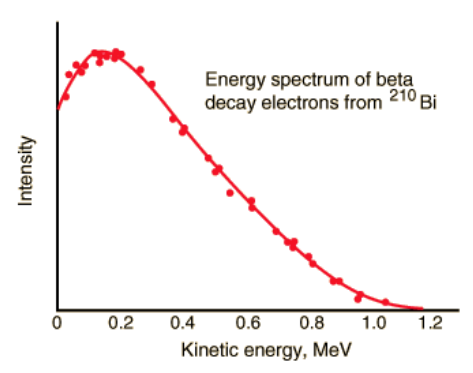
\includegraphics[width=10cm]{dec_beta_1.png}
\end{center}
L'andamento dello spettro in impulso degli elettroni risulta essere shiftato rispetto a quello dei positroni a causa dell'interazione coulombiana. 
\begin{center}
 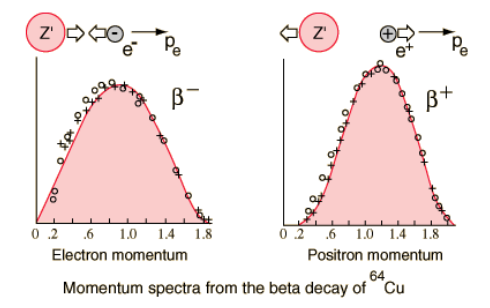
\includegraphics[width=8cm]{dec_beta_2.png}
\end{center}
\section{\texorpdfstring{Esempio: il decadimento doppio $^{90}\text{Sr}/^{90}\text{Y}$}{Esempio: il decadimento doppio 90Sr/90Y}} % Aggiunto \texorpdfstring per i segnalibri PDF
Il \textit{doppio decadimento} è un raro decadimento radioattivo in cui un nucleo decade in un altro con stesso numero di massa. Il doppio decadimento beta può essere interpretato come il verificarsi di due decadimenti beta contemporanei.\\ 
Un esempio è il decadimento doppio $^{90}Sr/^{90}Y$.
Esso consiste in due decadimenti $\beta^-$, dove nel primo lo \textit{Stronzio-90} decade in \textit{Ittirio-90} 
$$^{90}Sr\longrightarrow ^{90}Y$$
\begin{itemize}
    \item vita media $=27.7$ anni;
    \item $E_{max}= 0.546$ MeV.
\end{itemize}
L'Ittero a sua volta decade in \textit{Zirconio-90}
$$^{90}Y\longrightarrow ^{90}Zr$$
\begin{itemize}
    \item vita media $=64$ ore;
    \item $E_{max}= 2.27$ MeV.
\end{itemize}


\section{\texorpdfstring{Decadimento $\alpha$}{Decadimento alpha}} % Aggiunto \texorpdfstring per i segnalibri PDF
Il decadimento $\alpha$ è un decadimento che comporta l'emissione di una \textit{particella $\alpha$}, ossia un nucleo di $^4He$, cioè un sistema legato di due protoni e due neutroni. Il decadimento alfa è tipico dei radionuclidi che presentano un eccesso di protoni rispetto ai neutroni.\\ L'emissione di un tale cluster di nucleoni nel suo insieme piuttosto che l'emissione di singoli nucleoni è energeticamente più vantaggiosa a causa dell'energia di legame particolarmente elevata della particella $\alpha$. Il nucleo genitore (A, Z) nella reazione viene così trasformato tramite la legge:
$$(A,Z)\longrightarrow (A-4,Z-2)+\alpha$$
Com'è stato accennato poc'anzi, lo spettro del decadimento alfa è discreto in quanto si hanno dei
picchi del tipo:
\begin{center}
    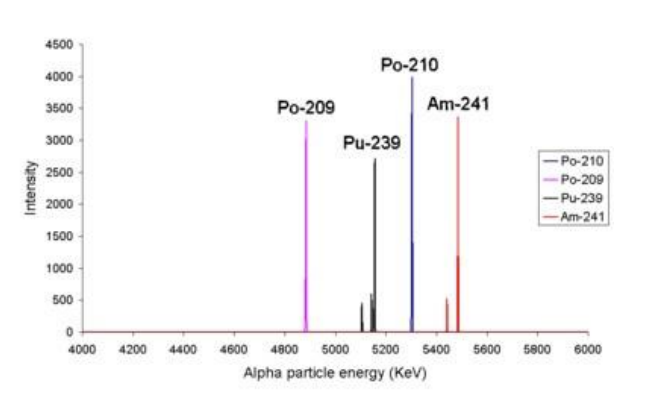
\includegraphics[width=8cm]{dec_alfa_1.png}
\end{center}
Poiché il decadimento alfa è un decadimento a due corpi il fascio di particelle alfa emesso è \textit{mono-energetico} ossia, fissato il nucleo padre, tutte le particelle alfa vengono emesse esattamente con la stessa energia.


\section{\texorpdfstring{Decadimento $\gamma$}{Decadimento gamma}} % Aggiunto \texorpdfstring per i segnalibri PDF
Così come gli elettroni di un atomo possono trovarsi su livelli energetici eccitati e diseccitandosi emettono fotoni così anche i nucleoni nel nucleo possono trovarsi su livelli energetici eccitati. In questi casi, dopo un intervallo di tempo brevissimo il nucleo compie una transizione dal livello eccitato ad un livello energetico inferiore ed emette un’energia sotto forma di radiazione elettromagnetica, in questo caso un fotone $\gamma$. Questo solitamente avviene in seguito ad un decadimento nucleare: tipicamente il nucleo figlio viene prodotto in uno stato eccitato e per portarsi
al livello fondamentale emette energia sotto forma di radiazione $\gamma$. Il decadimento $\gamma$ è dunque del
tipo:
$$^A_Z X^*\longrightarrow ^A_Z X + \gamma$$
dove con $^A_Z X^*$ si intende un nucleo nello stato eccitato.\\
Questo decadimento è dunque l’unico dei decadimenti radioattivi che non muta la specie chimica del nucleo di partenza.\\
Di seguito è riportato lo spettro gamma di un campione di Cesio-137, di Cobalto-60 ed infine di un campione contenente diversi isotopi emettitori gamma.
\begin{center}
    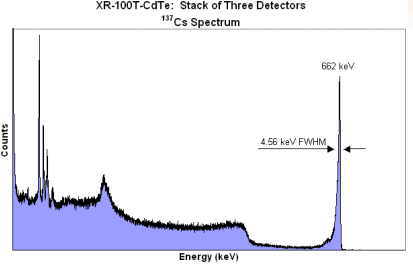
\includegraphics[width=8cm]{dec_gamma_cesio.png}
    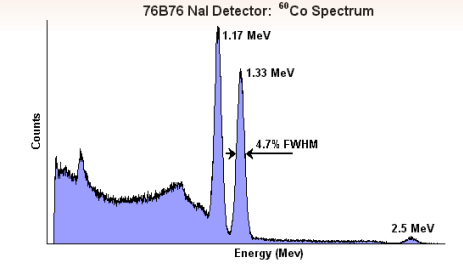
\includegraphics[width=8cm]{dec_gamma_cobalto.png}
\end{center}
\begin{center}
    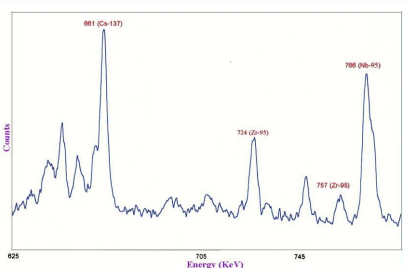
\includegraphics[width=8cm]{dec_gamma_vari.png}
\end{center}


\section{Fissione nucleare}
La fissione nucleare è il processo mediante il quale un nucleo pesante si scinde \textit{spontaneamente} in due nuclei aventi massa inferiore e energie molto elevate.\\
Talvolta durante il processo di fissione vengono emessi dei neutroni che tendono a innescare altre \textit{fissioni indotte} che danno luogo a una reazione a catena (processo tipico nell'esplosione della bomba atomica e nelle centrali nucleari).
\begin{center}
    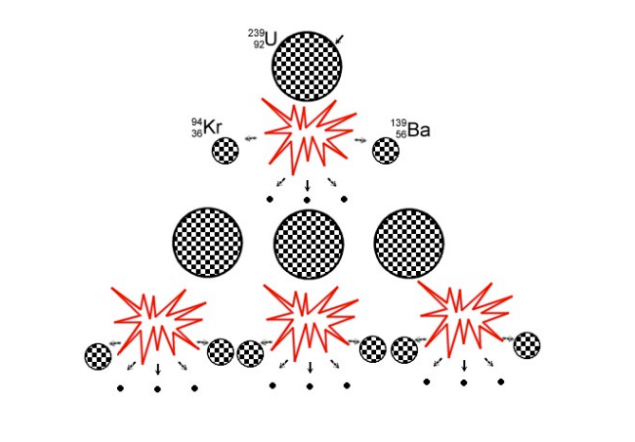
\includegraphics[width=9cm]{fissione_nucleare.png}
\end{center}

\section{Radiazione cosmica}
La \textit{radiazione cosmica} è causata da particelle estremamente energetiche provenienti dal Sole e dalle stelle che entrano nell'atmosfera terrestre. Alcune particelle arrivano a terra, mentre altre interagiscono con l’atmosfera per creare diversi tipi di radiazioni. I livelli di radiazione aumentano man mano che ci si avvicina alla sorgente, quindi la quantità di radiazione cosmica generalmente aumenta con l’elevazione. Maggiore è l’altitudine, maggiore è la dose. Questo è il motivo per cui coloro che vivono a Denver, in Colorado (altitudine di 1610 m) ricevono una dose annuale di radiazioni più elevata dalle radiazioni cosmiche rispetto a chi vive al livello del mare (altitudine di 0 m).
Al di là dell'atmosfera i raggi cosmici sono costituiti per circa il $90\%$ da protoni con un'energia fino e oltre $10^{20}$ eV e da nuclei di elio per quasi il $10\%$; tuttavia anche elettroni ed altri nuclei leggeri, fotoni, neutrini ed in minima parte positroni e antiprotoni fanno parte dei raggi cosmici primari.\\
Giunte nell'atmosfera terrestre, tali particelle interagiscono con i nuclei delle molecole dell'atmosfera formando così, in un processo a cascata, nuove particelle proiettate in avanti, che prendono il nome di \textit{raggi cosmici secondari}.\\
Le particelle più penetranti in questo sciame sono i muoni, capaci di arrivare anche al livello del mare.
\begin{center}
    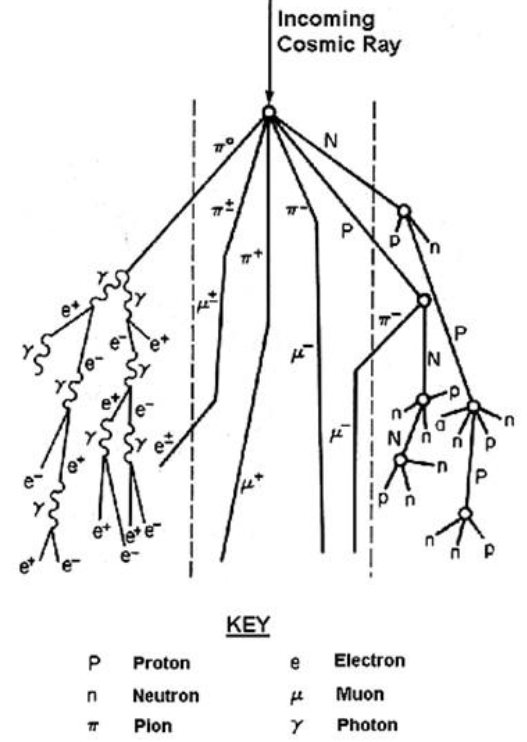
\includegraphics[width=5cm]{radiazione_cosmica.png}
\end{center}
Di seguito è riportato la distribuzione in energia dei cosmici primari
\begin{center}
    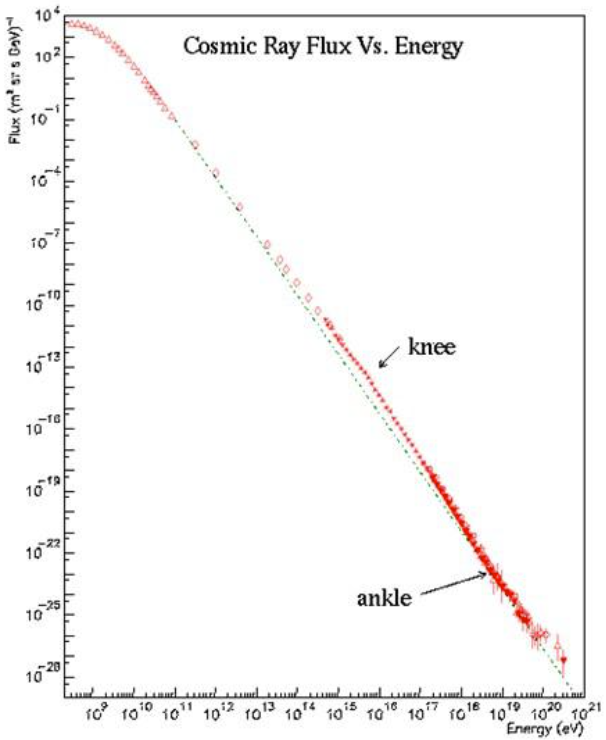
\includegraphics[width=5cm]{rad_cosm_1.png}
\end{center}

\section{Unità di misura e nomenclatura}
\begin{itemize}
    \item Attività: come detto precedentemente è il numero di decadimenti nell'unità di tempo. Si misura in:
    \begin{itemize}
        \item Bequerel: $1~~ Bq=1~~s^{-1}$;
        \item Curie: $1~~Ci=3.7*10^{10}~~Bq=3.7*10^{10}~~s^{-1}$;
        \item microCurie: $1~~\mu Ci= 37000~~Bq$
    \end{itemize}
    \item Dose: essa è l'energia depositata per unità di massa. Si misura in \textit{Gray}, $1~~Gy=\frac{1J}{1kg}$;
    \item Dose equivalente: misura il danno biologico provocato dall'assorbimento di radiazioni da parte di un intero organismo vivente, o anche di un singolo organo o tessuto. I diversi tipi di radiazione possono essere infatti più o meno dannosi per l'organismo. Si misura in \textit{sievert}, $1Sv=f*1Gy$, in sintesi 1 Sv, a differenza di 1 Gy, produce gli stessi effetti biologici indipendentemente dal tipo di radiazione considerata per cui non è più importante conoscere il tipo di radiazione assorbita. In alcune parti del mondo si utilizza la vecchia unità di misura, \textit{rem}, $1Sv=100rem$;
    \item Quality factor $f$: esso vale circa $1$ per $\gamma$ e $\beta$, circa $10$ per protoni e neutroni veloci, e circa $20$ per $\alpha$.
\end{itemize}
\section{Dosi tipiche}
Per quanto riguarda le sorgenti naturali:
\begin{itemize}
    \item radiazione cosmica: $28$ mrem/anno;
    \item fondo naturale: $26$ mrem/anno;
    \item radioattività interna al corpo: $26$ mrem/anno.
\end{itemize}
Invece per le sorgenti artificiali:
\begin{itemize}
    \item radiografia: variabile a seconda del tipo;
    \item RX torace: qualche mrem;
    \item TAC: $1000$ mrem;
\end{itemize}
I limiti tipici di dose per la popolazione è di circa $200-300$ mrem/anno, cioè $2-3$ mSv/anno.
\textbf{Esempio 1.}\\
In un volo Francoforte – San 
Francisco la dose assorbita da un passeggero a causa dei raggi cosmici può arrivare al $4\%$ della dose annua media assorbita da un individuo sulla Terra.
\textbf{Esempio 2.}\\
Gli astronauti sono esposti a diverse centinaia di mSv durante una missione di durata pari a 6 mesi.

\chapter{Perdita di energia-particelle cariche}
Il decadimento radioattivo è un insieme di processi fisico-atomici attraverso i quali alcuni nuclei atomici instabili (radionuclidi) decadono, in un certo tempo aleatorio detto tempo di decadimento, in nuclei di energia inferiore raggiungendo uno stato di maggiore stabilità con emissione di radiazioni ionizzanti in accordo ai principi di conservazione della massa/energia e della quantità di
moto. Il processo continua più o meno velocemente nel tempo fintantoché gli elementi via vi prodotti, che possono essere a loro volta radioattivi, non raggiungono una condizione di stabilità attraverso la cosiddetta catena di decadimento.\\
Col termine radiazione nucleare generalmente si intende una qualunque particella o radiazione elettromagnetica vera e propria emessa in una reazione nucleare artificiale o naturale; in tale termine vengono quindi comprese sia particelle atomiche e subatomiche (elettroni, protoni, muoni,
pioni, etc.), sia radiazioni elettromagnetiche quali raggi X e raggi $\gamma$.\\ 
Una classificazione può essere fatta tenendo conto della carica e della massa. In questo modo si possono distinguere quattro grandi
categorie:
\begin{itemize}
    \item[1)] particelle cariche pesanti;
    \item[2)] elettroni e positroni;
    \item[3)] fotoni;
    \item[4)] neutroni.
\end{itemize}
Ogni categoria si differenzia dall'altra per la diversa interazione con la materia di queste particelle, che dipende dalle loro caratteristiche intrinseche.
Per questo motivo si può stilare una lista di interazioni che fa riferimento alla classificazione precedentemente presentata:
\begin{itemize}
    \item[1)] Interazione di particelle cariche: Formula di Bethe – Bloch;
    \item[2)] Interazione di elettroni e positroni: collisione e bremsstrahlung;
    \item[3)] Interazione di raggi X e raggi $\gamma$: effetto fotoelettrico, effetto Compton, creazione di coppie;
    \item[4)] Interazione dei neutroni.
\end{itemize}
Per \textit{particelle cariche pesanti} si intendono particelle aventi massa intermedia tra quella degli elettroni e quella dei protoni (come i mesoni, che poi si dividono in muoni e pioni). Queste particolari particelle attraversando un materiale, possono perdere energia mediante due processi:
\begin{itemize}
    \item  Le collisioni anelastiche con gli elettroni atomici del materiale; queste essendo di natura Coulombiana danno come risultato la ionizzazione o l'eccitazione degli atomi del materiale; gli elettroni emessi possono ionizzare a loro volta. La massima energia trasferita nella singola interazione è di circa $4E \frac{m_e}{m}$, dove $m_e$ è la massa dell'elettrone e $m$ la massa della particella pesante. Per i protoni: $\frac{1}{500}$ di E (per perdere tutta la sua energia deve fare almeno 500 interazioni); la diminuzione della velocità/energia è continua.
    \item Lo scattering elastico dai nuclei, che produce il trasferimento di energia dalla particella agli atomi del materiale.
\end{itemize}
Fra i due il maggiore contributo alla perdita di energia lo dà il primo. Sia lo scattering elastico che quello anelastico sono dei processi di natura statistica, ma le fluttuazioni nella perdita di energia totale sono piccole se si considera la perdita di energia per unità di percorso, chiamata anche \textit{stopping power} o semplicemente $\frac{dE}{dx}$.\\

\section{Relazione di Bethe-Bloch}
Lo stopping power fu calcolato per la prima volta da Bohr usando argomenti classici e successivamente da Bethe-Bloch e altri usando la meccanica quantistica.\\
La formula di Bethe-Bloch descrive la perdita di energia media per unità di percorso. La formula ottenuta è quindi:
\begin{equation*}
    \medio{-\frac{dE}{dx}}=Kz^2\frac{Z}{A}\frac{1}{\beta^2}\Bigg[ \frac{1}{2} \log{\frac{2m_ec^2\beta^2\gamma^2W_{max}}{I^2}}-\beta^2-\frac{\delta(\beta\gamma)}{2} \Bigg]
\end{equation*}
La perdità di energia:
\begin{itemize}
    \item \'E proporzionale a $z^2$, ovvero alla carica della particella incidente (le particelle alfa perdono 4 volte più carica dei protoni), serve a identificare la partiecella;
    \item \'E proporzionale al rapporto $\frac{Z}{A}$, si ha maggiore perdita di energia sui nuclei leggeri in quanto questo rapporto è maggiore.
    \item dipende dall'energia della particella incidente, e se $\beta=\frac{v}{c}$ con vi piccolo allora possiamo dire che $\frac{1}{\beta^2}\propto\frac{1}{E}$;
\end{itemize}
Le grandezze riportate nella formula sono:
\begin{itemize}
    \item $K=4\pi N_A R_e^2 m_ec^2$ una costante che assume il valore di $0.307~~\frac{MeV ~ cm^2}{mol}$;
    \item $\rho$ è la densità del materiale usato come targhetta in $\frac{g}{cm^3}$;
    \item $z$ è il numero di carica della particella incidente;
    \item $Z$ è il numero atomico dell'elemento che costituisce la targhetta;
    \item $A$ è la massa atomica dell'elemento che costituisce la targhetta in $\frac{g}{mol}$;
    \item $c$ è la velocità della luce;
    \item $\beta$  è il il rapporto tra la velocità della particella incidente e la velocità della luce;
    \item $\gamma$ è il fattore di Lorentz ed è uguale a $\frac{1}{\sqrt{1-\beta^2}}$;
    \item $m_e$ è la massa dell'elettrone;
    \item $W_{max}=2m_ec^2\beta^2\gamma^2$ è l’energia massima trasferibile in una singola collisione della particella incidente;
    \item $I$ è il potenziale di eccitazione medio degli elettroni atomici del materiale espresso in $eV$; a seconda di $Z$, il valore di $I$ segue una delle seguenti formule:
    \begin{enumerate}
        \item per $Z<13 \implies I=Z(12+\frac{7}{Z})$ eV;
        \item per $Z\geq 13 \implies I=Z(9.76+58.8Z^{-1.19})$ eV;
    \end{enumerate}
    \item $\delta(\beta\gamma)$ è un fattore correttivo legato alla densità della targhetta, che può essere trascurato se $X < X_0$, con $X_0$ valore tabulato dipendente dal materiale del target e $X=\log(\beta \gamma)$.
\end{itemize}
In realtà vengono normalmente aggiunte due correzioni: la correzione dell'\textit{effetto densità} $\delta$ e la correzione della \textit{shell C}. La prima correzione deriva dal fatto che la particella carica tende a polarizzare gli atomi lungo il suo percorso. Ciò scherma l'interazione particella-elettrone. Questo effetto diventa più importante all'aumentare dell'energia della particella, ovviamnete dipende anche dal materiale che si sta attraversando.\\
La seconda correzione tiene conto degli effetti che si verificano quando la velocità della particella è paragonabile o inferiore alla velocità degli elettroni orbitanti. A basse energie l'ipotesi che l'elettrone sia stazionario rispetto alla particella non è più valida.\\
Per avere un'idea di seguito è riportato il grafico dell'andamento dello stopping power
\begin{center}
    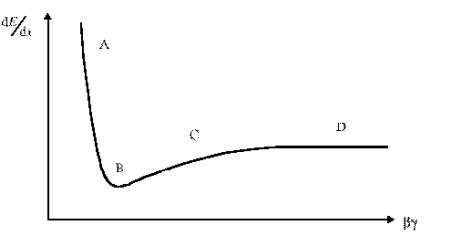
\includegraphics[width=10cm]{stopping_power.png}
\end{center}
Nel grafico sono evidenziate quattro zone:
\begin{itemize}
    \item Zona A: in tale regione si nota una ripida decrescita proporzionale a $\frac{1}{\beta^2}$;
    \item Punto B: qui si raggiunge un minimo di perdita di energia. Tale punto è conosciuto come minima ionizzazione. Per quanto riguarda quest'ultimo è noto che l'energia persa per ionizzazione da una particella carica in un mezzo è principalmente dipendete dalla sua velocità . Essa raggiunge un minimo che può essere considerato circa lo stesso per particelle pesanti con la stessa carica, mostrando quasi una totale indipendenza dalla massa. Spesso a tale minimo di ionizzazione viene data la sigla \textit{MIP};
    \item Zona C: in tale regione si ha una lenta crescita relativistica proporzionale a $\log\lambda$;
    \item Zona D: in tale regione la perdita di energia per unità di percorso diviene costante, poiché la ionizzazione è limitata dagli effetti di densità.
\end{itemize}
Se si divide l'equazione di Bethe-Bloch per la densità $\rho$ si ottiene la perdita di energia per unità di densità superficiale:
$$\frac{1}{\rho}\frac{dE}{dx}$$
espressa in $MeV\frac{cm^2}{g}$.\\
La perdita di energia in un composto si valuta mediante la legge:
$$\frac{1}{\rho}\frac{dE}{dx}=\sum_i \Bigg( \frac{n_iA_i}{\rho_i A} \bigg(\frac{dE}{dx}\bigg)_i\Bigg)$$
dove $n_i$ è il numero di atomi della specie i nel composto, $A_i$ è il peso atomico della specie i, $\rho_i$ la densità della specie i e $\bigg(\frac{dE}{dx}\bigg)_i$ la perdita di energia della specie i.

\section{Curve di Bragg}
È stato notato che la perdita di energia varia man mano che la particella penetra nel materiale, raggiungendo un massimo ad una determinata profondità. Le curve che mostrano la dipendenza di $dE/dx$ dalla penetrazione della particella nel materiale vengono chiamate \textit{curve di Bragg}. La loro conoscenza diventa molto utile nelle applicazioni mediche delle radiazioni, ad ad esempio quando si vogliono colpire delle cellule tumorali con un minimo di danno per i tessuti sani circostanti
\begin{center}
    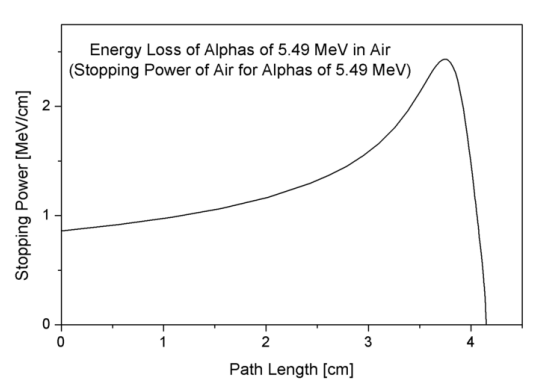
\includegraphics[width=8cm]{picco_bragg.png}
\end{center}
La perdita di energia per particelle cariche pesanti solitamente è distribuita attorno ad un valore medio. Tale distribuzione, che con termine tecnico viene definita \textit{straggling energetico}, è
approssimativamente una gaussiana per assorbitori più spessi, invece tende a sviluppare una coda verso più alte energia man mano che diminuisce lo spessore, con un andamento asimmetrico descritto dalla
distribuzione di Landau.
\begin{center}
    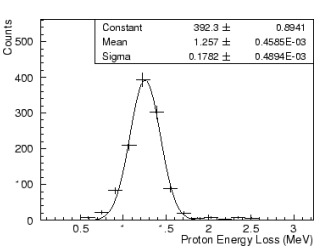
\includegraphics[width=7cm]{bb_1.png}
    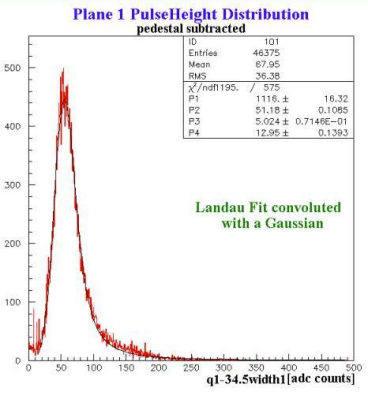
\includegraphics[width=7cm]{bb_2.png}
\end{center}

\section{Range di una particella}
Il \textit{range di una particella} è la distanza da essa percorsa in un materiale, prima di perdere tutta la propria energia. 
$$range=\int_0^{E_0}\bigg(\frac{dE}{dx}\bigg)^{-1}dE$$
con $E_0$ energia iniziale; essa è molto simile alla formula che mi permette di calcolare la perdita di energia in uno spessore x:
$$\int_0^{x}\frac{dE}{dx}dx$$
Questa quantità dipende dal tipo di particella, dalla sua energia e dal tipo di materiale. In teoria per particelle identiche, con la stessa energia iniziale e nelle stesso materiale, il range dovrebbe essere uguale; ma ciò non è vero, a causa delle fluttuazioni statistiche (\textit{straggling}), dovute al fatto che ogni particella non subisce lo stesso numero di collisioni e quindi l'energia a parità di condizioni iniziale non viene persa allo stesso modo. 
Sperimentalmente questa quantità può essere calcolata facendo passare un fascio di particella della stessa energia attraverso diversi spessori di uno stesso materiale, in modo da vedere come varia il rapporto tra le particelle trasmesse e le particelle incidenti. Un'idea dell'andamento di una curva ottenuta con tale sistema è data nel grafico che segue:
\begin{center}
    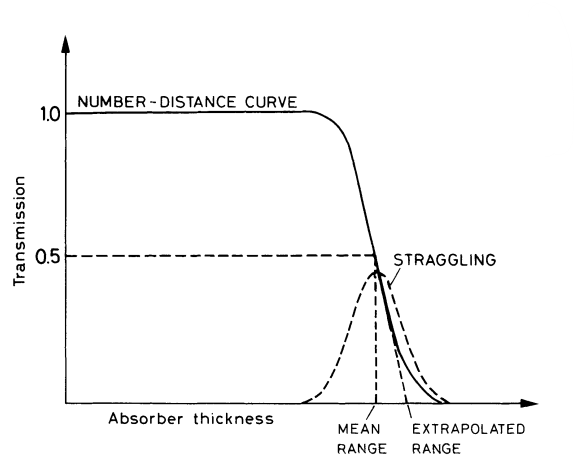
\includegraphics[width=8cm]{bb_3.png}
\end{center}
Come è evidenziato in figura, il valore per cui la trasmissione si riduce al $50\%$ è conosciuto come “\textit{range medio}”, corrisponde al valore medio della gaussiana, curva che mi descrive la distribuzione delle distanze percorse; esso corrisponde appunto alla distanza in cui la metà delle particelle del fascio vengono assorbite. Più comunemente, però, come valore di range viene preso il punto di intersezione della tangente condotta dal valore della curva corrispondente al range medio con l'asse $\Vec{x}$, tale valore prende il nome di “\textit{range estrapolato}”. Se non vi fossero fluttuazioni si avrebbe un "gradino" netto, nella realtà è smussato.

\section{Radiazione Cherenkov}
L'emissione di radiazione Cherenkov si verifica quando una particella carica viaggia in un mezzo con una velocità superiore a quella della luce nello stesso mezzo. Questa velocità è data da:
$$\beta c =v=\frac{c}{n}$$
dove n è l'indice di rifrazione e c è la velocità della luce.\\
In un mezzo con indice di rifrazione $n(\omega)$ il campo elettrico generato da una particella carica all'interno del mezzo polarizza linearmente il mezzo stesso mentre si propaga con velocità $v_{particella}$. Se la velocità della particella nel mezzo è inferiore allora non vi è perdita di energia da parte della particella, ma se $v_{particella}>\frac{c}{n}$ il materiale polarizzato emette radiazione. Il motivo di tale emissione è legato alla polarizzazione e depolarizzazione del mezzo, che genera lungo la traccia una serie di onde sferiche il cui
inviluppo costituisce un fronte d’onda conico, con un angolo ben definito 
$$\theta_c=\arccos\frac{1}{\beta n(\omega)}$$
rispetto alla traiettoria della particella. Si noti che questo angolo dipende dalla velocità della particella e dalla frequenza della radiazione emessa.
\begin{center}
    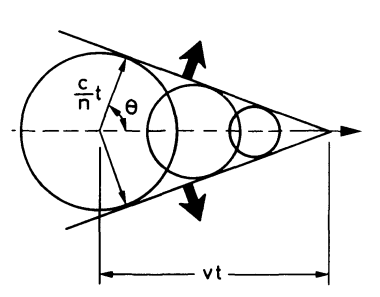
\includegraphics[width=6cm]{emissione_cherenkov.png}
\end{center}
Il numero di fotoni emessi per unità di percorso (e quindi l'energia persa) dipendono da $\theta_c$. Risulta che l'energia persa per effetto Cherenkov è 
$$\frac{dE}{dx}\approx z^2\sin^2\theta_c$$
cioè trascurabile rispetto quella persa per collisione.\\
Lo spettro di emissione è continuo in frequenza, nel range del visibile è maggiore nel blu.\\
Il rilevamento di radiazione Chrenkov è oggi sfruttato nell'astronomia delle sorgenti gamma e negli esperimenti condotti sui neutrini, rilevando ad esempio i muoni prodotti in acqua, i quali, essendo negativamente carichi, e viaggiando a una velocità superiore a quella di propagazione della luce in acqua, danno luogo all'effetto Cherenkov. Inoltre, è impiegata nei reattori nucleari a immersione, in quanto l'intensità della radiazione è correlata alla frequenza degli eventi di fissione, ed è quindi indicativa del livello di attività del reattore. Viene usata anche in campo biologico per rintracciare piccole quantità e basse concentrazioni di biomolecole.

%dalla slide 15 alla slide viene spiegato l'esercitazione da svolgere con root

\chapter{Perdita di energia-elettroni}
Come le particelle cariche pesanti, anche gli elettroni e i positroni subiscono una perdita di energia per collisione quando attraversano la materia. Tuttavia, a causa della loro piccola massa, entra in gioco un ulteriore meccanismo di perdita di energia: \textit{bremsstrahlung}. 

\section{Bremsstrahlung}
Il bremsstrahlung è una radiazione elettromagnetica che viene prodotta a causa della decelerazione di una particella carica, tipicamente un elettrone, deviata da un’altra particella carica, tipicamente il nucleo atomico; il fenomeno è noto anche come \textit{radiazione di frenamento}; infatti, supponendo che vi siano particelle cariche in una porzione di materia e che un elettrone ad alta velocità ci passi vicino, la traiettoria di quest’ultimo verrà deviata a causa del campo elettrico attorno al nucleo atomico.\\
A energie di pochi MeV o meno, questo processo  risulta ininfluente. Tuttavia, all'aumentare dell'energia, la probabilità di bremsstrahlung aumenta rapidamente così che a pochi decine MeV la perdita di energia per irraggiamento è paragonabile o maggiore rispetto alla perdita per collisionale. A energie superiori a questa energia critica, bremsstrahlung domina completamente.
\begin{center}
    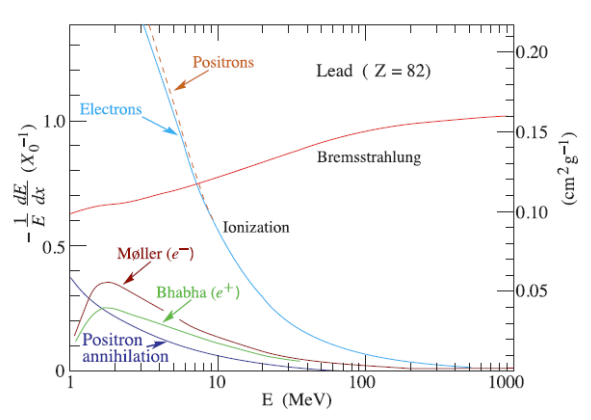
\includegraphics[width=10cm]{bremsstraqualcosa.png}
\end{center}
\section{Perdita di energia}
La perdita totale di energia di elettroni e positroni, quindi, è composta da due termini: quello di frenamento e quello di collisione.
$$\bigg( \frac{dE}{dx}\bigg)_{tot}=\bigg( \frac{dE}{dx}\bigg)_{rad}+\bigg( \frac{dE}{dx}\bigg)_{coll}$$

\section{Termine collisionale}
Mentre il meccanismo di base della perdita per collisione delineato per le particelle cariche pesanti è valido anche per elettroni e positroni, la formula di Bethe-Bloch deve essere leggermente modificata per due ragioni. Uno, essendo la loro massa piccola l'ipotesi che la particella incidente rimanga non deviata durante il processo di collisione non è quindi valida, si ha un moto disordinato. La seconda è che per gli elettroni le collisioni sono tra particelle identiche, per cui il calcolo deve tener conto della loro indistinguibilità. Queste considerazioni cambiano alcuni termini nella formula, in particolare la massima energia persa in una ionizzazione diventa $W_{max}=\frac{T_e}{2}$, dove $T_e$ è l'energia cinetica dell'elettrone o del positrone incidente. Rifacendo il calcolo, allora la formula di Bethe-Bloch diventa
$$-\frac{dE}{dx}=2\pi N_a r^2_e m_e c^2\rho \frac{Z}{A}\frac{1}{\beta^2}\bigg[ \ln{\frac{\tau^2(\tau +2)}{2(I/m_e c^2)^2}}+F(\tau)-\delta -2\frac{C}{Z} \bigg]$$
dove $\tau$ è l'energia cinetica della particella in unità di $m_e c^2$, la funzione $F(\tau)$ assume un valore differente a seconda del tipo di particella:
$$F(\tau)_{e^-}=1-\beta^2+\frac{\frac{\tau^2}{8}-(2\tau-1)\ln{2}}{(\tau+1)^2}$$
$$F(\tau)_{e^+}=2\ln{2}-\frac{\beta^2}{12}\bigg( 23+\frac{14}{(\tau+2)}+\frac{10}{(\tau+2)^2}+\frac{4}{(\tau+2)^3}\bigg)$$

\section{Termine di frenamento}
Una particella carica decelerata emette radiazione, con una sezione d'urto
$$\frac{d\sigma}{dE}\propto \frac{Z^2}{m^2_i}\frac{\ln{E}}{E}$$
dipende non solo dall'energia dell'elettrone incidente, ma anche dal numero atomico, Z, del materiale e dalla massa della particella incidente. \'E utile osservare che più grande è la massa della particella più piccola è la sezione d'urto.\\
Il contributo dovuto alla radiazione di frenamento, può ora essere calcolata integrando la sezione d'urto:
$$-\frac{dE}{dx}=4Z^2r^2_e \alpha \bigg[\ln{\bigg(183Z^{-1/3}+\frac{1}{18}\bigg)}-f(Z)\bigg]NE$$
Questo contributo è trascurabile per particelle più pesanti dell'elettrone (di un fattore $\bigg( \frac{m_e}{m}\bigg)^2$, già per i muoni $\bigg( \frac{m_e}{m}\bigg)^2=\frac{1}{37000}$).

\section{Energia critica}
L'energia persa per radiazione dipende fortemente dal materiale su cui incide l'elettrone (o il positrone) ed è quindi interessante conoscere per ciascun materiale l'energia critica, $E_c$, alla quale l'energia persa per collisione eguaglia quella persa per radiazione nel processo di bremsstrahlung. Questo avviene quando:
$$\bigg( \frac{dE}{dx}\bigg)_{rad}=\bigg( \frac{dE}{dx}\bigg)_{col}$$
per $E=E_c$.\\
Al di sopra di questa energia, la perdita di radiazione è dominante rispetto a quella per collisone e viceversa sotto $E_c$.\\
Il valore di $E_c$ è stato parametrizzato a partire dai dati sperimentali. Essa vale:
\begin{itemize}
    \item Per i gas: $\frac{610MeV}{Z+1.24}$
    \item Per i solidi: $\frac{710MeV}{Z+0.92}$
\end{itemize}
\begin{center}
    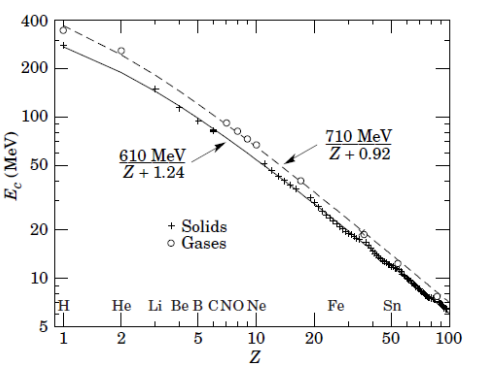
\includegraphics[width=9cm]{energia_critica_elettrone.png}
\end{center}

\newpage
\section{Range dell'elettrone}
A causa della maggiore suscettibilità dell'elettrone allo scattering multiplo da parte dei nuclei, il range degli elettroni è generalmente molto diverso dalla lunghezza del percorso calcolata ottenuta da un'integrazione della formula $\frac{dE}{dx}$
$$range\neq \int\bigg(\frac{dE}{dx}\bigg)^{-1}dE$$
Spesso si riscontrano differenze che vanno dal $20\%$ al $400\%$ a seconda dell'energia e del materiale. Inoltre, la perdita di energia da parte degli elettroni oscilla molto di più che per le particelle pesanti. Ciò è dovuto al trasferimento di energia molto maggiore per collisione consentito per gli elettroni e all'emissione di bremsstrahlung. In entrambi i casi è possibile che pochi urti singoli assorbano la maggior parte dell'energia dell'elettrone. Ciò, ovviamente, si traduce in effetti di straggling energetici maggiori (non presenta più il "gradino"), come illustrato nella figura che mostra alcune curve di range misurate.
\begin{center}
    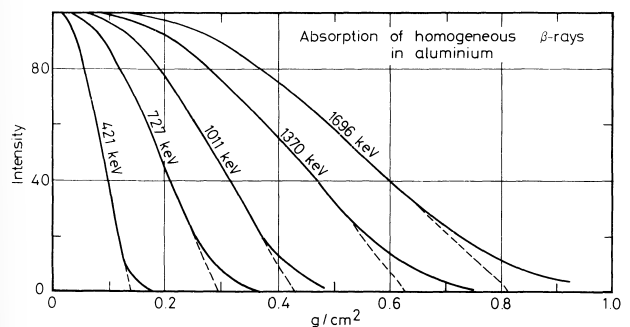
\includegraphics[width=10cm]{range_e_1.png}
\end{center}
A causa del loro spettro continuo di energie, l'assorbimento degli elettroni del decadimento $\beta$ mostra un comportamento che è molto ben approssimato da una forma esponenziale del tipo:
$$I=I_0 e^{-\mu x}$$
Ciò è illustrato nella figura seguente che mostra le curve numero-distanza per diversi assorbitori tracciate su una scala semi-logaritmica.
\begin{center}
    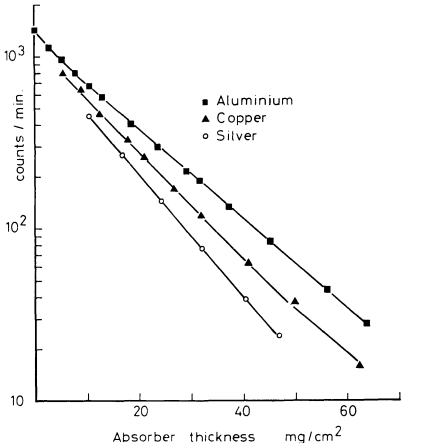
\includegraphics[width=8cm]{range_e_3.png}
\end{center}
La costante $\mu$ è nota come \textit{coefficiente di assorbimento beta} e risulta essere direttamente correlata all'energia finale del decadimento. 

\section{Backscattering}
A causa della sua piccola massa, gli elettroni sono particolarmente suscettibili alle grandi deviazioni angolari dovute alla dispersione dai nuclei. Questa probabilità è così alta, infatti, che gli elettroni soggetti a scattering multiplo possono essere completamente invertiti nella direzione, in modo che vengano retrodiffusi fuori dall'assorbitore. Ciò è illustrato schematicamente nella seguente.
\begin{center}
    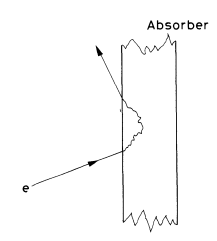
\includegraphics[width=4cm]{backscattering_1.png}
\end{center}
L'effetto è particolarmente forte per gli elettroni a bassa energia e aumenta con il numero atomico Z del materiale.\\ 
Il\textit{ backscattering} dipende anche dall'angolo di incidenza. Ovviamente gli elettroni che entrano ad angoli obliqui rispetto alla superficie dell'assorbitore hanno una maggiore probabilità di essere dispersi rispetto a quelli incidenti lungo la perpendicolare.\\
Il rapporto tra il numero di elettroni retrodiffusi e gli elettroni incidenti è noto come \textit{coefficiente di backscattering} o \textit{albedo}. La figura successiva mostra alcuni coefficienti misurati per vari materiali in funzione dell'energia incidente.
\begin{center}
    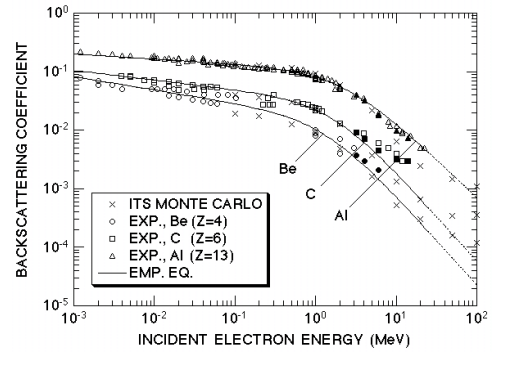
\includegraphics[width=8cm]{backscattering_2.png}
    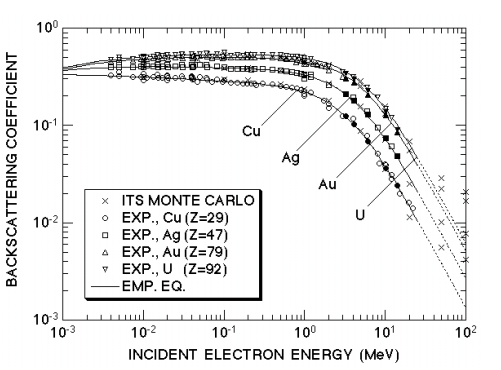
\includegraphics[width=8cm]{backscattering_3.png}
\end{center}
Il backscattering è importante per i rivelatori di elettroni in cui, a seconda della geometria e dell'energia, una grande frazione di elettroni può essere dispersa prima di essere in grado di produrre un segnale utilizzabile.\\
Per gli elettroni non collimati su un materiale ad alto Z come \textit{NaI}, ad esempio, fino all'$80\%$ può essere riflesso indietro.

\section{Scattering multiplo}
Una particella carica che attraversa un mezzo è deflessa attraverso tanti piccoli processi di scattering.\\
Il maggior contributo a questa deflessione è dato da processi Coulombiani e in misura minore anche dalla interazione nucleare.\\
Queste deflessioni sono regolate individualmente dalla ben nota formula di Rutherford:
$$\frac{d\sigma}{d\Omega}=z_2^2z^2_1r_e^2 \frac{(m_e c/\beta p)^2}{4\sin^4(\theta/2)}$$
essendovi una dipendenza da $\frac{1}{\sin^4(\theta/2)}$ la stragrande maggioranza di queste collisioni si traduce, quindi, in una piccola deflessione angolare della particella.\\
Possiamo dividere i processi Coulombiani in tre tipologie:
\begin{itemize}
    \item \textit{Single scattering}: Se l'assorbitore è molto sottile tale che la probabilità di più di uno scattering di Coulomb è piccola, descrivibile dalla formula di Rutherford;
    \item \textit{Plural scattering}: Se il numero medio di scattering $N < 20$, allora abbiamo il plural scattering. Questo è il caso più difficile da trattare poiché né la semplice formula di Rutherford né i metodi statistici possono essere semplicemente applicati. Alcuni lavori in questa regione sono stati svolti da Keil;
    \item \textit{Multiple scattering}: Se il numero medio di scattering è $N > 20$ e la perdita di energia è piccola o trascurabile, il problema può essere trattato statisticamente per ottenere una distribuzione di probabilità dell'angolo netto di deflessione in funzione dello spessore del materiale attraversato. 
\end{itemize}
In generale, il calcolo rigoroso dello scattering multiplo è estremamente complicato ed esistono diverse formulazioni e formule più o meno sofisticate.
Tra le più usate vi è la teoria di Molière.\\La distribuzione dell'angolo di scattering
\begin{itemize}
    \item è una Gaussiana per piccoli angoli;
    \item per angoli grandi ha una coda con valori al di sopra della funzione Gaussiana.
\end{itemize}
La deflessione può essere valutata nello spazio (angolo relativo tra direzione di moto originaria e direzione dopo aver attraversato un dato spessore) oppure nel piano (proiezione su un piano).\\
La deviazione media nel piano è $0$. Le deviazioni quadratiche medie di queste 
quantità sono legate da:
$$\theta_0=\theta_{plane}^{rms}=\frac{1}{\sqrt{2}}\theta_{space}^{rms}$$
L'ammontare dello scattering multiplo dipende
\begin{itemize}
    \item dal tipo di particella carica incidente;
    \item dall'enrgia (o dall'impulso) della particella incidente;
    \item dalle proprietà del materiale.
\end{itemize}
Assumendo una distribuzione Gaussiana per l’angolo di scattering nel piano, la sua larghezza è data da:
$$\theta_0=\frac{13.6MeV}{\beta cp}z\sqrt{\frac{x}{X_0}}\bigg[ 1+0.038\ln{\frac{x}{X_0}}\bigg]$$
dove
\begin{itemize}
    \item $p$ è l'impulso della particella;
    \item $z$ è il numero atomico della particella;
    \item $x$ è lo spessore del materiale;
    \item $X_0$ è la lunghezza di radiazione del materiale.
\end{itemize}

\section{Lunghezza di radiazione}
Molto spesso per gli elettroni anziché parlare di distanze percorse in un mezzo si preferisce ragionare in termini di \textit{lunghezza di radiazione} $X_0$. Questo parametro può essere definito come
\begin{itemize}
    \item La distanza media entro cui un elettrone di alta energia riduce la sua energia ad $1/e$;
    \item I $7/9$ del libero cammino medio per produzione di coppie da parte di un fotone di alta energia del valore iniziale mediante processi di emissione di radiazione.
\end{itemize}
In altri termini, $X_0$ è una lunghezza caratteristica che descrive lo sviluppo dei processi elettromagnetici in un materiale.\\
La lunghezza di radiazione può essre valutata a partire dalle caratteristiche del materiale attraverso formule empiriche:
$$L_{rad}=\frac{716.4 g/cm^2A}{Z(Z+1)\ln(287/\sqrt{Z})}(g/cm^2)$$
dove $Z$ e $A$ sono rispettivamente il numero atomico e il peso del materiale. Di seguito vi è una tabella con i valori tipici di alcuni materiali:
\begin{center}
    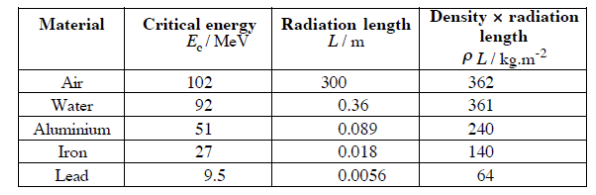
\includegraphics[width=12cm]{lungh_rad.png}
\end{center}

\section{Distribuzione angolare}
Dato il valore di $\theta_0$ la distribuzione dell'angolo di scattering è data, nello spazio, da:
$$\frac{1}{2\pi\theta_0^2}\exp\bigg( -\frac{\theta^2_{space}}{2\theta^2_0}\bigg)d\Omega$$
mentre, nel piano, da:
$$\frac{1}{\sqrt{2\pi}\theta_0^2}\exp\bigg( -\frac{\theta^2_{plane}}{2\theta^2_0}\bigg)d\theta_{plane}$$

La traiettoria di una particella carica viene leggermente modificata, per cui la direzione che eventualmente misuriamo mediante un rivelatore non è quella originaria
Esempi:
\begin{itemize}
    \item[a)] rivelatori di tracciamento in esperimenti a LHC;
    \item[b)] ricostruzione direzione dei muoni cosmici;
    \item[c)] ...
\end{itemize}
L’effetto dello scattering multiplo è
\begin{itemize}
    \item più importante per particelle di basso impulso;
    \item più importante per materiali ad alto Z.
\end{itemize}
Talvolta lo scattering multiplo è utile per valutare le caratteristiche del materiale attraversato (tomografia muonica).

\section{Tomografia muonica}
La \textit{tomografia muonica} è una tecnica che utilizza i muoni per ricostruire un’immagine della struttura interna di un oggetto anche molto grande.\\ 
Mentre i raggi X non riescono ad attraversare più di qualche decina di centimetri, i muoni possono attraversare grandi spessori di materia, anche alcuni chilometri. Questa caratteristica permette di impiegare queste particelle per realizzare immagini tridimensionali di strutture di grandi dimensioni dall’esterno e in completa sicurezza.
\begin{center}
    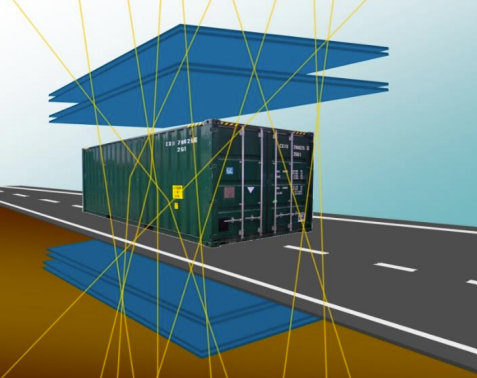
\includegraphics[width=9cm]{tom_mu_1.png}
    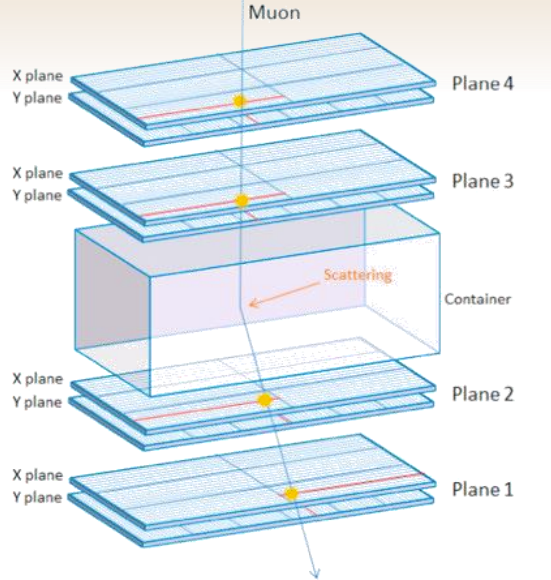
\includegraphics[width=9cm]{tom_mu_2.png}
\end{center}

\chapter{Iterazione gamma-materia}
Il comportamento dei fotoni nella materia (raggi $X$ e raggi $\gamma$) è radicalmente diverso da quello delle particelle cariche. In particolare, la mancanza di carica elettrica del fotone rende impossibili collisioni elastiche e anelastiche con gli elettroni atomici del mezzo assorbitore. 
Invece, le principali interazioni dei raggi $X$ e dei raggi $\gamma$ nella materia sono:
\begin{itemize}
    \item[-] Effetto fotoelettrico;
    \item[-] Effetto Compton;
    \item[-] Creazione di coppia.
\end{itemize}
Le sezioni d'urto di questi tre processi sono molto più piccole di quelle che descrivono le interazioni delle particelle cariche e sono caratterizzate da una grande dipendenza dall'energia iniziale del fascio di fotoni.\\
Ognuno dei tre processi elimina o devia il fotone dalla direzione del fascio, quindi i fotoni che vengono rivelati lungo tale direzione dopo aver attraversato il mezzo sono quelli che non hanno subito nessuna interazione e quindi possiedono l'energia originale.
L'attenuazione del fascio dipende dal numero di fotoni che hanno interagito ed ha un andamento di tipo esponenziale:
$$I = I_0 e^{-\mu x}$$

dove $I_0$ è l'intensità del fascio incidente, $x$ lo spessore dell'assorbitore, $I$ è l'intensità del fascio dopo lo spessore $x$ e $\mu$ il coefficiente di assorbimento.
Il coefficiente di assorbimento è dato da:
$$\mu=N\sigma_{tot}=\frac{N_a\rho}{A}\sigma_{tot}$$
dove $N$ è la densità di atomi nell'assorbitore e $\sigma_{tot}$ la sezione d'urto totale per atomo, dovuta al contributo dei 3 processi secondo la formula:
$$\sigma_{tot}=\sigma_{phot}+Z\sigma_{Compton}+\sigma_{coppie}$$
dove $Z$, numero atomico dell'assorbitore, moltiplica $\sigma_{Compton}$ in modo da considerare gli $Z$ elettroni per
atomo.\\
Nei grafici successivi vengono rappresentate le sezioni d’urto dei vari processi di interazione dei gamma in funzione dell’energia.
\begin{center}
    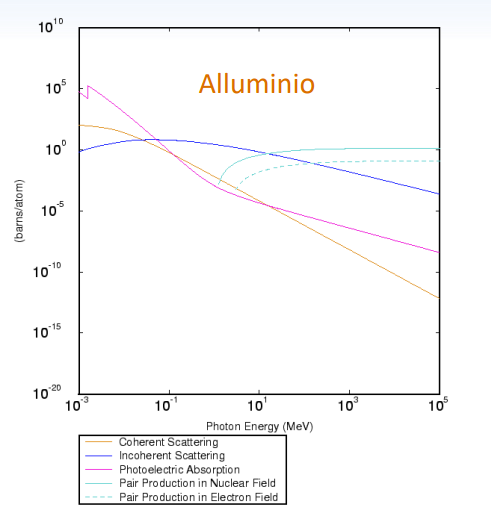
\includegraphics[width=8cm]{gamma_all.png}
    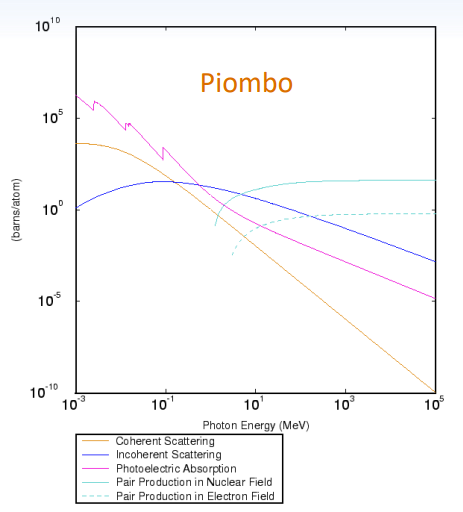
\includegraphics[width=8cm]{gamma_pio.png}
\end{center}
Nel grafico successivo è rappresentato il coefficiente di assorbimento in funzione dell’energia
\begin{center}
    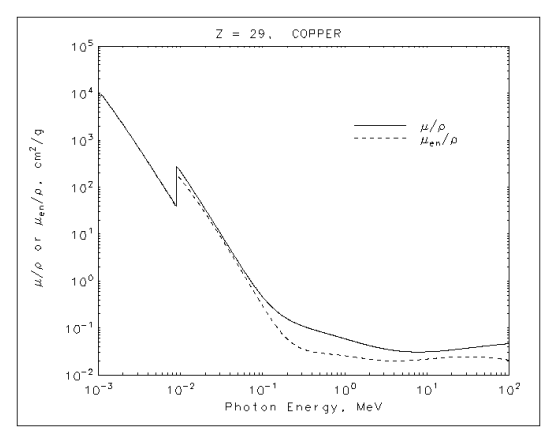
\includegraphics[width=9cm]{gamma_ass.png}
\end{center}

\newpage
\section{Effetto fotoelettrico}
L'\textit{effetto fotoelettrico} spiega l'emissione di elettroni da parte di un metallo colpito da una radiazione elettromagnetica. 
\begin{center}
    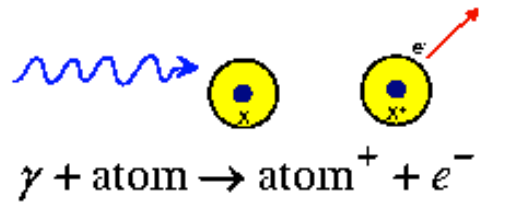
\includegraphics[width=3cm]{eff_fotoell.png}
\end{center}
La spiegazione di tale fenomeno fu un successo della meccanica quantistica e fu resa possibile quando nel 1905 Einstein estese le ipotesi quantistiche di Planck, postulando che la quantizzazione non era una proprietà  del meccanismo di emissione, ma piuttosto una proprietà intrinseca del campo elettromagnetico.\\
Usando questa ipotesi Einstein fu capace di spiegare il fenomeno osservato nell'effetto fotoelettrico, cioè il fatto che l'energia cinetica con cui venivano emessi gli elettroni variava con la frequenza della radiazione incidente secondo la relazione:
$$K_{max}=h\nu-W_0$$
dove $h$ è la costante di Planck, $W_0$ è l'energia caratteristica associata ad ogni dato metallo e chiamata
\textit{energia di estrazione}, $c$ la velocità della luce e $\nu$ è la frequenza della radiazione incidente.\\
Questo è il risultato aspettato se i fotoni hanno un'energia quantizzata pari a $E=h\nu$, che è il valore
proposto da Einstein. Nell'approssimazione $h\nu << mc^2$, la sezione d'urto per effetto fotoelettrico
vale:
$$\sigma_{phot}=4\alpha^4\sqrt{2}Z^5\Phi_0\sqrt{\frac{m_ec^2}{h\nu}}$$
Come si nota dalla formula la sezione d'urto per effetto fotoelettrico dipende principalmente dal numero atomico $Z$ e diminuisce man mano che aumenta l'energia.
Nella figura sottostante si può vedere l'andamento della sezione d'urto, calcolata per il piombo.
\begin{center}
    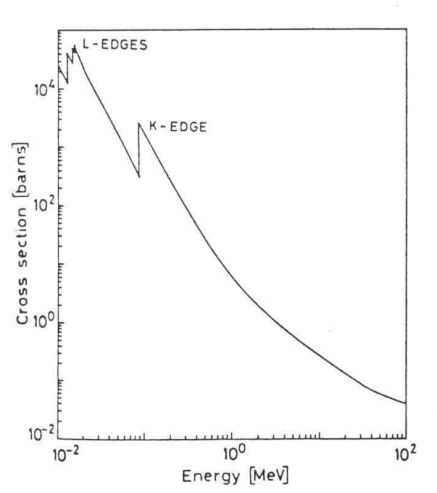
\includegraphics[width=7cm]{eff_fotoell1.png}
\end{center}
Il processo fotoelettrico è importante a basse energie, mentre decresce velocemente con l'aumentare dell’energia del fotone.

%\newpage
\section{Effetto Compton}
Lo \textit{scattering Compton} avviene su elettroni liberi non legati al nucleo, contrariamente all'effetto fotoelettrico. Nella materia, naturalmente, gli elettroni sono legati; tuttavia, se l'energia del fotone è elevata rispetto all'energia di legame, quest'ultima può essere ignorata e gli elettroni possono essere considerati essenzialmente liberi.\\
Nell'interazione, il fotone di energia $h\nu$ trasferisce ad un elettrone, che si suppone fermo, parte della
sua energia e del suo impulso. Come risultato si avrà un fotone diffuso ad un angolo $\theta$ con un
energia $h\nu'$, e l'elettrone deflesso ad un angolo $\varphi$ con energia cinetica $T$.
\begin{center}
    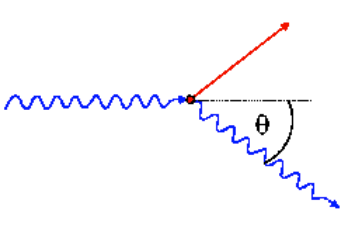
\includegraphics[width=4cm]{compton.png}
\end{center}
Applicando la legge di conservazione dell'energia e della quantità di moto si ottengono le seguenti relazioni:
$$h\nu'=\frac{h\nu}{1+\gamma(1-\cos\theta)}$$
$$T=h\nu-h\nu'=h\nu\frac{\gamma(1-\cos\theta)}{1+\gamma(1-\cos\theta)}$$
con $\gamma=\frac{h\nu}{m_e c^2}$.\\
La sezione d'urto è data da:
\begin{center}
    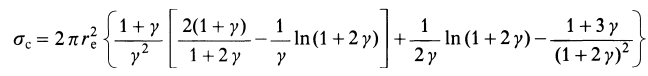
\includegraphics[width=12cm]{compton2.png}
\end{center}
Tale sezione d'urto si può decomporre in due termini: il primo $\sigma^a$ è la sezione d'urto d'assorbimento Compton, che è proporzionale all'energia media trasferita all'elettrone di rinculo, mentre il secondo $\sigma^s$ è proporzionale alla frazione di energia totale del fotone diffuso. Queste due quantità possono essere calcolate dalla formula di Klein-Nishina. Pertanto:
$$\sigma_{compton}=\sigma^a + \sigma^s$$
Nella figura sottostante si può vedere l'andamento delle sezioni d'urto $\sigma_{compton}$, $\sigma^a$ e $\sigma^s$:
\begin{center}
    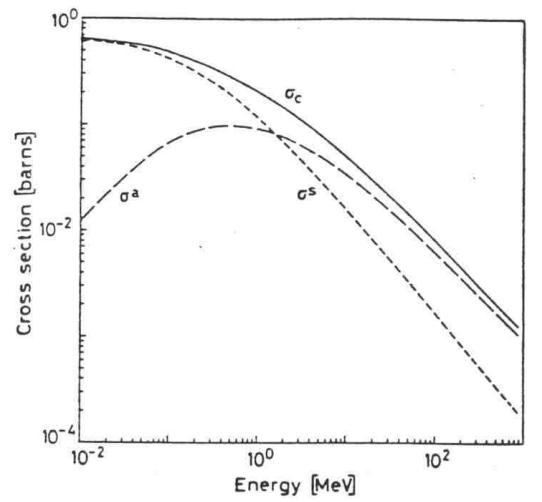
\includegraphics[width=8cm]{compton1.png}
\end{center}
Si osserva che:
\begin{itemize}
    \item La sezione d’urto per effetto Compton prevale a energie intermedie e decresce all'aumentare dell'energia del fotone;
    \item Dipende da Z;
    \item Ad alte energie vi è una dipendenza da $\frac{\ln E}{E}$.
\end{itemize}

%\newpage
\section{Creazione di coppia}
La \textit{creazione di coppia} implica la trasformazione del fotone
incidente in una coppia elettrone-positrone.\\ 
Il processo può avvenire solo quando l'energia del fotone è pari almeno alla
somma delle masse delle particelle create, cioè per $E_{\gamma}=2m_e c^2$, ossia superiore a $1.022 MeV$ e in presenza di un terzo corpo, in genere un nucleo, affinché ci sia conservazione della quantità di moto.
\begin{center}
    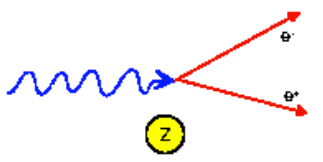
\includegraphics[width=4cm]{coppiaee.png}
\end{center}
Per la conservazione dell'energia si ha:
$$T(e^-)+T(e^+)=h\nu + 2m_e c^2$$
dove $h\nu$ è l'energia del fotone incidente e la differenza a secondo membro fornisce l'energia cinetica che viene ripartita fra le particelle. Quando l'energia cinetica del positrone diventa bassa (confrontabile con l'energia termica degli elettroni nel mezzo) esso si ricombina con un elettrone dando luogo a due fotoni che sono emessi in direzioni opposte, ciascuno con energia pari a $0.51 ~~MeV$. Successivamente questi due fotoni possono essere riassorbiti per effetto fotoelettrico o Compton.\\
La sezione d'urto per produzione di coppia vale:
$$\sigma_{coppia}=4Z^2\alpha r^2_e \Bigg[ \frac{7}{9}\bigg( \ln{\frac{2h\nu}{m_e c^2}}-f(Z) \bigg)-\frac{109}{54} \Bigg]$$
dove $Z$ è il numero atomico del materiale assorbitore, $\alpha$ è la costante di struttura fine e la funzione $f(Z)$ è una piccola correzione coulombiana, che tiene conto dell'interazione dell'elettrone nel campo del nucleo.\\
La sezione d'urto per creazione di coppie cresce rapidamente all'aumentare dell'energia dei fotoni incidenti, divenendo ad alte energie l'unico processo efficace per l'assorbimento dei fotoni.
\begin{center}
    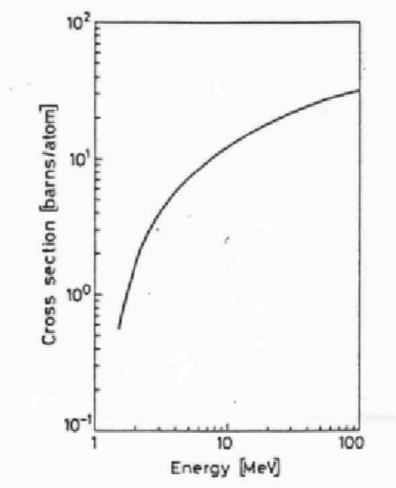
\includegraphics[width=8cm]{coppiaee1.png}
\end{center}

\section{Ricapitolando}
\begin{itemize}
    \item A basse energie, dell'oridine dei $MeV$, i fotoni interagiscono in prevalenza mediante l'effetto fotoelettrico;
    \item A energie dell'ordine delle decine di $MeV$ tende a prevalere l'effetto Compton;
    \item Ad alte energie, superiori circa a $10MeV$, il processo prevalente è quello di produzioene di coppia elettrone-positrone.
\end{itemize}

\chapter{Sciami elettromagnetici}
Uno dei risultati più impressionanti dell'effetto combinato della produzione di coppia da parte di fotoni ad alta energia e dell'emissione di bremsstrahlung da parte di elettroni è la formazione di \textit{sciami elettromanetici}. Un fotone ad alta energia nella materia si converte in una coppia di elettroni e positroni che poi emettono fotoni energetici di bremsstrahlung. Questi, a loro volta, si convertono in ulteriori coppie $e^+$ $e^-$ e così via. Il risultato è una cascata o pioggia di fotoni, elettroni e positroni. Ciò continua fino a quando l'energia degli elettroni e dei positroni prodotti dalla coppia scende al di sotto dell'energia critica. A questo punto, le coppie $e^+$ $e^-$ preferenzialmente perderanno la loro energia per collisioni atomiche, effetto fotoelettrico e Compton piuttosto che per emissione di bremsstrahlung, arrestando così la cascata.\\
Lo sviluppo della cascata è, ovviamente, un processo statistico. Utilizzando la nozione di lunghezza della radiazione, tuttavia, possiamo costruire un semplice modello per descrivere il numero medio di particelle prodotte e le loro energie medie in funzione della profondità di penetrazione nel materiale che viene attraversato. Supponiamo di iniziare con un fotone energetico di energia $E_0$. In media, quindi, il fotone si convertirà in una coppia $e^+$ $e^-$ dopo una lunghezza di radiazione. L'energia di ciascun membro della coppia è quindi $E_0/2$. Dopo due lunghezze di radiazione, l'elettrone e il positrone emetteranno ciascuno un fotone bremsstrahlung con circa la metà dell'energia della particella carica. A questo punto ci sono $4$ particelle
presenti: due fotoni e una coppia elettrone-positrone, ciascuno con energia $E_0/4$. Alla fine di tre lunghezze di radiazione, i fotoni di bremsstrahlung si saranno convertiti in altre due coppie $e^+$ $e^-$, mentre la coppia originale avrà emesso un altro set di fotoni di bremsstrahlung. Il numero di particelle presenti è quindi $8$ e la loro energia $E_0/4$.
\begin{center}
    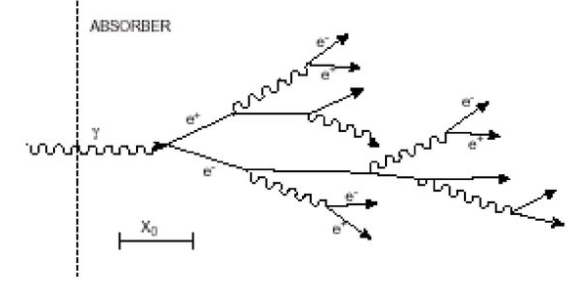
\includegraphics[width=8cm]{scaime_ele.png}
\end{center}
Continuando in questo modo, è facile vedere che alla fine di $t$ lunghezze di radiazione\footnote{Si può considerare $t$ come il rapporto tra la distanza $x$ dal "punto di partenza" e la lunghezza di radiazione $X_0$.}, il numero totale di particelle (cioè fotoni, elettroni e positroni) presenti sarà
$$N\simeq 2^t$$
Ognuna avente energia in media pari a: 
$$E(t)=\frac{E_0}{2^t}$$
Quando l’energia media delle particelle diviene eguale all'energia critica
$$\frac{E_0}{2^t}=E_c$$
non verranno più prodotte nuove particelle e lo sciame non si sviluppa ulteriormente.\\ 
Questo avviene quando il numero di generazioni $t$ è tale che
$$\frac{E_0}{E_c}=2^t \implies t=\frac{\ln{\frac{E_0}{E_c}}}{\ln 2}$$
Il numero massimo di particelle prodotte è quindi $N\simeq\frac{E_0}{E_c}$.\\
Questo semplice modello, tuttavia, fornisce solo un quadro qualitativo approssimativo dello sciame.
Per effettuare un calcolo più preciso è utile ricorrere a tecniche come le simulazioni Monte Carlo.\\
La figura seguente mostra i risultati di uno di questi calcoli per uno sciame di $30 GeV$ nel ferro. 
\begin{center}
    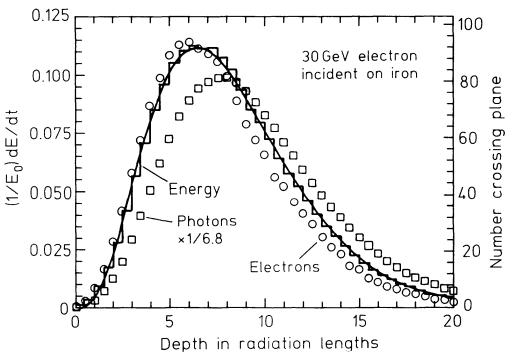
\includegraphics[width=8cm]{sciame_ele2.png}
\end{center}
I cerchi e i quadrati danno essenzialmente il numero di elettroni e fotoni, rispettivamente, in funzione della profondità nel ferro, mentre l'istogramma descrive l'energia depositata dallo sciame, cioè $dE/dt$.\\
Si è osservato che circa il 95\% di uno sciame è contenuto logitudinalmente entro 20 lunghezze di radiazione. Nel grafico seguente si può vedere la perdita in percentuale di energia di una cascata elettromagnetica in funzione di $X_0$:
\begin{center}
    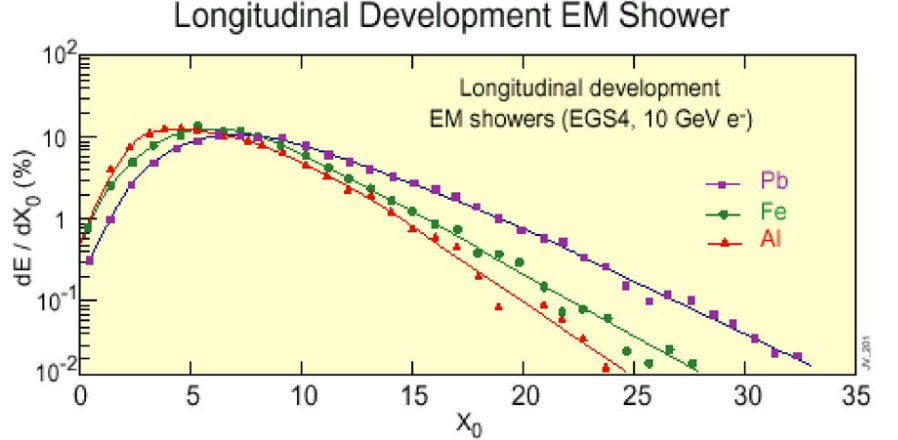
\includegraphics[width=10cm]{sciame_ele1.png}
\end{center}
Man mano che lo sciame penetra in profondità dentro un materiale, esso si allarga anche trasversalmente.\\
L’allargamento trasversale è descritto dal \textit{raggio di Molière}, un parametro legato alle proprietà del materiale da una relazione approssimata del tipo
$$R_M=0.0265X_0(Z+1.2)$$
Le figure successive illustrano il profilo di perdita di energia trasversale per uno sciame calcolata a varie profondità. 
\begin{center}
    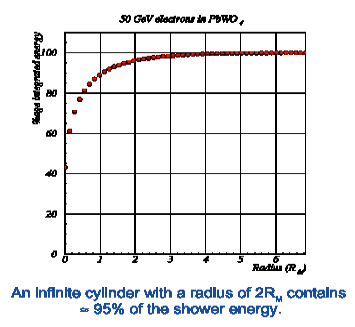
\includegraphics[width=7cm]{sciame_3.png}
    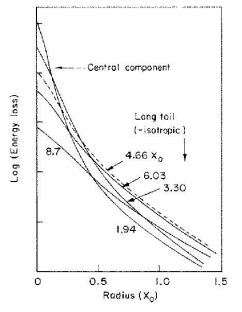
\includegraphics[width=7cm]{scaime_4.png}
\end{center}
Qualitativamente, possiamo vedere che la cascata rimane relativamente stretta nelle prime lunghezze di radiazione del suo sviluppo con la maggior parte delle particelle contenute in un denso nucleo centrale. Attorno a questa regione centrale c'è un tenue alone di particelle che si estende verso l'esterno a distanze relativamente grandi. Man mano che la pioggia avanza, tuttavia, il nucleo centrale si disperde, scomparendo infine dopo aver raggiunto il massimo.\\
Più del $95\%$ della doccia è comunque contenuta entro una distanza di circa $2R_M$ dall'asse longitudinale.


\chapter{Rilevatori di particelle}
Affinché un \textit{rivelatore} sia capace di rilevare una particella o una radiazione, occorre innanzitutto che queste interagiscano con il rilevatore stesso attraverso uno dei meccanismi discussi in
precedenza. Un importante aspetto da valutare è il cosiddetto “\textit{tempo di volo}” della particella.
Questo tempo è confrontabile con il tempo d risposta del rivelatore che talvolta è anche minore del \textit{tempo d'interazione}. Quest'ultimo è il tempo necessario per arrestare una particella carica o per lo sviluppo di uno sciame di particelle ed è dell'ordine dei nanosecondi nei gas e dei picosecondi nei solidi.\\
Le eventuali cariche prodotte nel rivelatore verranno poi raccolte in tempi caratteristici di ogni tipologia di rivelatore (dai ns ai ms).
L'interazione con il rivelatore darà luogo quindi ad una successione di segnali prodotti dalla particella o dalla radiazione incidente in istanti di tempo del tutto casuali e con intensità variabile.
Tali conteggi seguono una distribuzione governata dalla statistica di Poisson.\\
Si possono distinguere due modi di rivelazione:
\begin{itemize}
    \item \textit{Pulsed mode}: il rivelatore rivela singoli impulsi;
    \item \textit{Current mode}: il rivelatore non distingue i singoli impulsi ma ne fornisce una media.
\end{itemize}
Il segnale prodotto in un rilevatore può fornire diverse informazioni:
\begin{itemize}
    \item \textit{Ampiezza}: l'ampiezza dei vari segnali può essere diversa a seconda dell'energia della particella incidente, a seconda dell'interazione con il rilevatore o per effetto delle fluttuazioni statistiche;
    \item \textit{Tempo di arrivo}: il tempo associato al segnale fornisce informazioni sul tempo di arrivo della particella e può essere usato per diverse applicazioni;
    \item \textit{Forma e durata}: la durata di un segnale può essere diversa a seconda della risposta del rivelatore e avere una forma che dipende anche da tipo di particella.
\end{itemize}
I segnali forniti da un rivelatori si suddividono in due grandi categorie:
\begin{itemize}
    \item \textit{Segnali Analogici}: è un segnale continuo nel tempo che può assumere tutti gli infiniti valori della grandezza fisica osservabile contenuti all'interno di un range, cioè tra un minimo relativo ed un massimo relativo;
    \item \textit{Segnali Digitali}: è un segnale che all'interno di un range può assumere solo un numero discreto (numerabile) di valori.
\end{itemize}
\section{Analisi delle ampiezze}
In genere durante le esperienze di rivelazione, si effettua un'analisi delle ampiezze, cioè uno studio della distribuzione delle ampiezze dei segnali.\\
La distribuzione delle ampiezze dei segnali può essere utilizzata per avere informazioni sulla distribuzione delle particelle che incidono sul rilevatore o sui processi fisici che avvengono
all'interno del rilevatore stesso.\\
Si può costruire un istogramma riportando le ampiezze $H$ di un dato segnale in funzione del tempo $t$ e poi studiare la distribuzione delle ampiezze graficando lo spettro $\frac{dN}{dH}$ in funzione delle $H$ espresse in canali di acquisizione (spettro discreto).\\
Un esempio di spettro delle ampiezze misurate in un rivelatore a scintillazione letto da un fotomoltiplicatore, in presenza di una sorgente gamma di $^{137}Cs$.
\begin{center}
    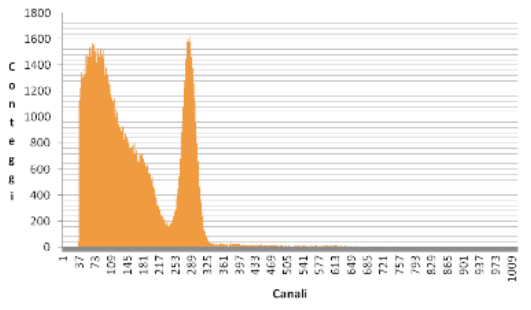
\includegraphics[width=9cm]{Cs_riv.png}
\end{center}
Grazie ad uno spettro di questo tipo si possono trarre le seguenti informazioni:
\begin{itemize}
    \item Numero di segnali complessivi (integrale dello spettro);
    \item Numero di segnali compresi tra due valori (integrale tra due limiti fissati, ad esempio intorno ad un picco);
    \item Forma dello spettro;
    \item Presenza di picchi;
    \item Valore massimo delle ampiezze.
\end{itemize}

\section{Distribuzione delle ampiezze}
Molto spesso, l'ampiezza di un segnale è proporzionale all'energia depositata nel rivelatore.\\ 
Lo spettro delle ampiezze può dunque essere convertito in uno spettro in energia con una opportuna \textit{calibrazione}.
La calibrazione di uno spettro si effettua tramite il best-fit dell'energia in funzione dei canali.
\begin{center}
    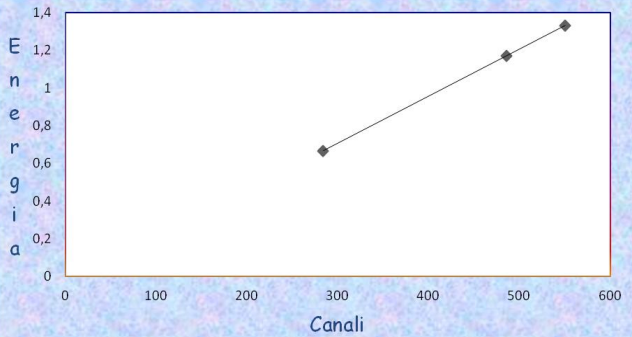
\includegraphics[width=9cm]{riv_best.png}
\end{center}
La linearità è la principale qualità di un rilevatore di particelle e consiste nella proprietà di dare una risposta direttamente correlata alle energia della particella o della radiazione incidente. Non sempre la corrispondenza tra ampiezze misurate ed energia è lineare! Effetti di non linearità possono derivare dal funzionamento del rivelatore.\\
Un esempio di spettro ottenuto con un rivelatore al silicio mediante una sorgente alfa con tre picchi di energia nota e la corrispondente retta di taratura ottenuta tramite best-fit sono riportati in figura:
\begin{center}
    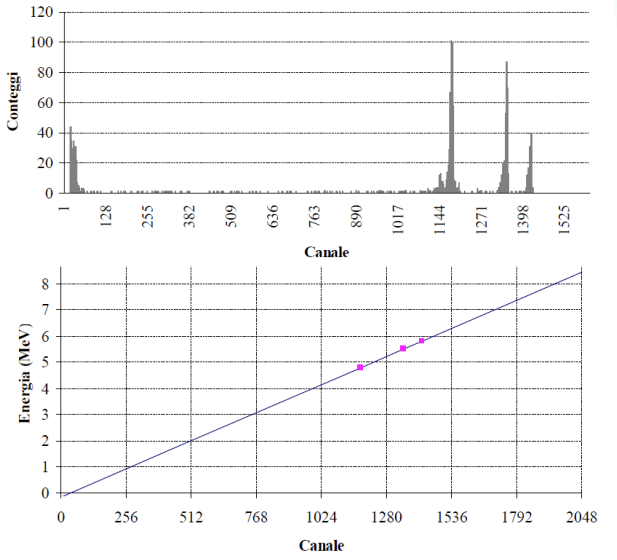
\includegraphics[width=9cm]{calibrazione_riv.png}
\end{center}

\newpage
\section{Risoluzione in energia}
Per i rivelatori uno dei fattori più importante è la \textit{risoluzione energetica}. Essa è legata alla capacità di distinguere radiazioni che depositano nel rivelatore energie simili tra loro.\\
In generale, la risoluzione può essere misurata inviando un raggio di radiazione monoenergetica nel rivelatore e osservando lo spettro risultante. Idealmente, ovviamente, si dorrebbe vedere una delta di Dirac. In realtà, si osserva una struttura di picco con una larghezza finita, solitamente di forma gaussiana. Questa larghezza nasce a causa delle fluttuazioni nel numero di ionizzazioni ed eccitazioni prodotte.
\begin{center}
    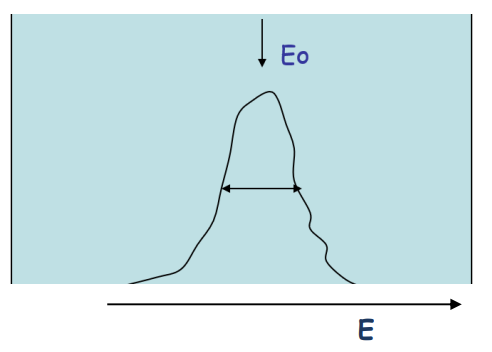
\includegraphics[width=6cm]{alt_met.png}
\end{center}
La risoluzione è generalmente data in termini di larghezza del picco a metà altezza (\textit{FWHM}). Le energie che sono più vicine di questo intervallo sono generalmente considerate irrisolvibili.\\
La risoluzione è definita come il rapporto tra la larghezza a metà altezza del picco divisa per il valore centrale $E_0$:
$$R=\frac{FWHM}{E_0}$$
che è solitamente espressa in percentuale.\\
Ad esempio, un rivelatore $NaI$ ha una risoluzione dell'$8\%$ o del $9\%$ per i raggi $\gamma$ di circa $1 MeV$, mentre i rivelatori al germanio hanno risoluzioni dell'ordine dello $0,1\%$!\\
In generale, la risoluzione è una funzione dell'energia depositata nel rivelatore che migliora all'aumentare dell'energia. 
\begin{center}
    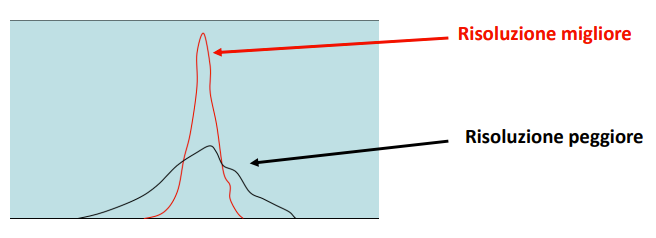
\includegraphics[width=8cm]{alt_met_2.png}
\end{center}
La risposta di un rivelatore può essere soggetta a fluttuazioni dovute a rumori casuali della strumentazioni e a fluttuazioni statistiche. 
Il disturbo statistico è intrinseco, in quanto i portatori di carica nei rilevatori sono entità discrete (coppie di ioni, elettroni,...), soggetti a fluttuazioni anche a parità di energia depositata.\\
Può essere effettuata una stima della fluttuazione intrinseca, assumendo che la formazione di ciascun portatore di carica sia un processo poissoniano.\\
Per calcolare le fluttuazioni è necessario considerare due casi.

\section{Primo caso: l'energia non è totalmente assorbita}
Per un rivelatore in cui l'energia della radiazione non è totalmente assorbita, per esempio un sottile rivelatore che misura solo la perdita $dE/dx$ di una particella che passa, il numero di reazioni che producono il segnale è dato da una distribuzione di Poisson. La varianza è quindi data da
$$\sigma^2=J$$
dove $J$ è il numero medio di eventi prodotti.\\ 
Si può quindi vedere la dipendenza energetica della risoluzione
$$R=2.35\frac{\sqrt{J}}{J}=2.35\sqrt{\frac{w}{E}}$$
dove il fattore $2,35$ mette in relazione la deviazione standard di una gaussiana con il suo FWHM. Quindi la risoluzione varia inversamente alla radice quadrata dell'energia.

\section{Secondo caso: energia totalmente assorbita}
Se l'intera energia della radiazione viene assorbita, come nel caso dei rivelatori usati negli esperimenti di spettroscopia, la statistica di Poisson non è applicabile. Si osserva che la risoluzione di molti di questi rivelatori è in realtà inferiore a quella calcolata dalle statistiche di Poisson.\\ 
La differenza qui è che l'energia totale depositata è un valore fisso e costante, mentre nel caso precedente l'energia depositata può fluttuare.\\ 
Il numero totale di ionizzazioni che possono verificarsi e l'energia persa in ciascuna ionizzazione sono quindi vincolati da questo valore. Statisticamente, ciò significa che gli eventi di ionizzazione non sono tutti indipendenti, quindi la statistica di Poisson non è applicabile. Fano è stato il primo a calcolare la varianza in questa condizione e a trovarla
$$\sigma=FJ$$
dove $J$ è la ionizzazione media prodotta e $F$ è un numero noto come \textit{fattore Fano}.\\
Il fattore $F$ è una funzione di tutti i vari processi fondamentali che possono portare a un trasferimento di energia nel rivelatore ed è una costante intrinseca del materiale. Teoricamente, $F$ è molto difficile da calcolare con precisione in quanto richiede una conoscenza dettagliata di tutte le reazioni che possono avvenire nel rivelatore.\\
La risoluzione, in questo caso, è data da:
$$R=2.35\frac{\sqrt{FJ}}{J}=2.35\sqrt{\frac{Fw}{E}}$$
Nella maggior parte dei rilevatori $F<1$.

\section{Esempio}
Spettro di particelle alfa misurato con un rivelatore al silicio
    $$R=\frac{150keV}{10.9MeV}=1.4\%$$
    \begin{center}
       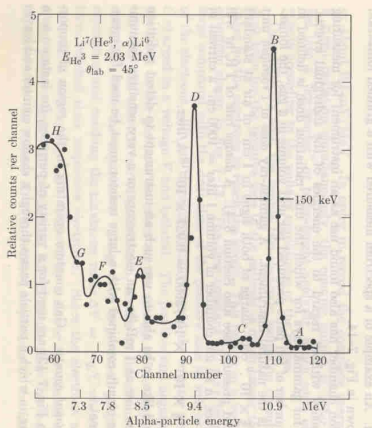
\includegraphics[width=4cm]{risa1.png}
    \end{center}
 
\section{Efficienza intrinseca}
Non tutte le particelle o le radiazioni che colpiscono un rivelatore sono in grado di dare un segnale misurabile. Ogni rivelatore ha una sua \textit{efficienza intrinseca} di rivelazione, data dal rapporto fra il numero di particelle rivelate e il numero di quelle incidenti.
$$\varepsilon_{int}=\frac{numero~particelle ~rivelate}{numero~particelle~incidenti}$$
L'efficienza intrinseca dipende in generale da:
\begin{itemize}
    \item dal tipo di particella o radiazione incidente;
    \item energia della particella;
    \item Tipo di rivelatore;
    \item Volume del rivelatore.
\end{itemize}
Un ulteriore fattore per valutare le prestazioni di un rivelatore è l'\textit{accettanza geometrica} che dipende dall'angolo solido con cui il rilevatore vede la sorgente. Questa grandezza è data dal rapporto tra il numero di particelle che colpiscono il rilevatore ed il numero di particelle emesse dalla sorgente
$$\varepsilon_{geometrica}=\frac{numero~particelle ~rivelate}{numero~particelle~emesse}$$
Questo è dovuto al fatto che nonostante una sorgente puntiforme emetta isotropicamente in tutto l'angolo solido solo una frazione di esse interagirà con il rilevatore.\\
In generale il calcolo dell'accettanza geometrica è di tipo probabilistico e non esistendo soluzioni analitiche al problema si fa uso di simulazioni numeriche quali il metodo Monte Carlo. Per quanto
concerne, invece, il calcolo dell'angolo solido, esso comporta una integrazione delle funzioni di Bessel mediante metodi numerici.\\
L'efficienza complessiva è data dal prodotto delle due efficienze:
$$\varepsilon_{tot}=\varepsilon_{geometrica}*\varepsilon_{intrinsica}$$
Conoscendo l'efficienza complessiva, si possono correggere i dati misurati per valutare le quantità originali.

\section{Tempo di risposta}
Il segnale fornito da un rivelatore può dare informazioni sul tempo di arrivo della particella o della radiazione. La risoluzione temporale esprime l'indeterminazione nella conoscenza del tempo di arrivo.\\
La risoluzione temporale dipende da:
\begin{itemize}
    \item Tipo di rivelatore;
    \item Modo di funzionamento del rivelatore;
    \item Dimensioni del rivelatore;
    \item Elettronica associata per la trattazione del segnale.
\end{itemize}
In molti casi è importante avere una buona risoluzione temporale.\\
Tipicamente hanno risoluzioni temporali estremamente buone, ovvero dell'ordine dei 100 picosecondi, i rivelatori a gas del tipo Parallel Plate e MPRC.\\
I rivelatori a gas del tipo camere a ionizzazione, contatori proporzionali, Geiger producono, invece, segnali lenti, ovvero dell'ordine dei microsecondi, e hanno risoluzioni temporali scadenti.\\
Infine i rilevatori basati su scintillatori di piccole dimensioni hanno risoluzioni dell'ordine del nanosecondo.

\section{Tempo morto}
In una successione di eventi misurati da un rivelatore, esiste un tempo minimo tra due venti successivi, al di sotto del quale il rilevatore non può separarli.\\
Questo tempo è il \textit{tempo morto} del sistema ed è appunto il tempo che impiega un certo apparato di misura, dopo aver ricevuto uno stimolo esterno, ad essere pronto per eseguire correttamente una
nuova misura.
\begin{center}
    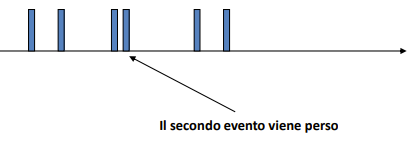
\includegraphics[width=8cm]{tempomorto.png}
\end{center}
Poiché l'arrivo degli eventi è casuale (statistica di Poisson) la probabilità che due eventi arrivino separati da un intervallo inferiore del tempo morto non è mai nulla.\\
Il tempo morto di un sistema dipende, oltre che dalle caratteristiche intrinseche del rilevatore, anche dal rate di conteggio. Si può diminuire se la risposta dei rivelatori è veloce.\\
Possiamo distinguere due tipologie di tempo morto
\begin{itemize}
    \item \textit{Paralizzabile}: l'apparato non registra l'evento, ma si generano delle modifiche nello stato e quindi il tempo morto si prolunga. Un evento che avviene durante il tempo morto dopo il precedente non solo è perso, ma fa ricominciare il conteggio del tempo morto, quindi aumentando il rate sul rilevatore questo raggiungerà un punto di saturazione nel quale non sarà in grado di registrare nessun evento;
    \begin{center}
       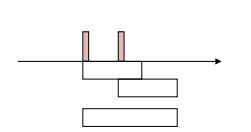
\includegraphics[width=6cm]{tempomorto3.png}
    \end{center}
    \item \textit{Non Paralizzabile}: l'apparato non registra l'evento e non modifica il suo stato.
    \begin{center}
       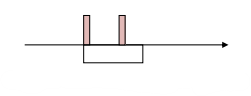
\includegraphics[width=6cm]{tempomorto2.png}
    \end{center}
\end{itemize}
Il tempo morto influisce sul rate di conteggi in quanto causa la perdita dell'acquisizione di alcuni eventi. A seconda che il tempo morto sia paralizzabile o meno è possibile correggerlo nel modo che segue, posto $\tau$ il tempo morto ed $R$ il rate di conteggio:
\begin{itemize}
    \item \textit{Non Paralizzabile}: $R_{vero}=\frac{R_{misurato}}{1-R_{misurato}\tau}$;
    \item \textit{Paralizzabile}: $R_{misurato}=R_{vero}e^{-R_{vero}\tau}$.
\end{itemize}
Per bassi valori di rate ($R_{vero}<<1/\tau$) entrambi i casi forniscono l'approssiamzione:
$$R_{misurato}=R_{vero}(1-R_{vero})$$

\section{Esempio 1: Tempo morto di 10 microsecondi}
\begin{center}
    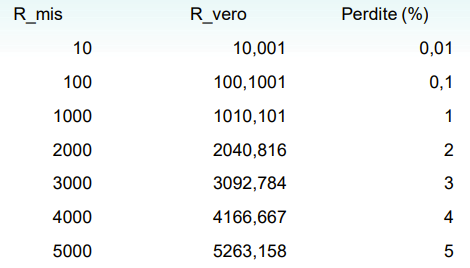
\includegraphics[width=8cm]{esmorto1.png}
\end{center}

\section{Esempio 2: Tempo morto di 100 microsecondi}
\begin{center}
    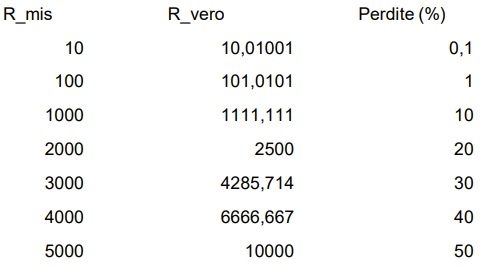
\includegraphics[width=8cm]{esmorto2.png}
\end{center}

\section{Andamento del rate}
In figura è riportato l'andamento del rate osservato in funzione del rate vero e nella seconda figura l'andamento del rate osservato in funzione del rate vero, per diversi valori di tempo morto (caso non paralizzabile).
\begin{center}
    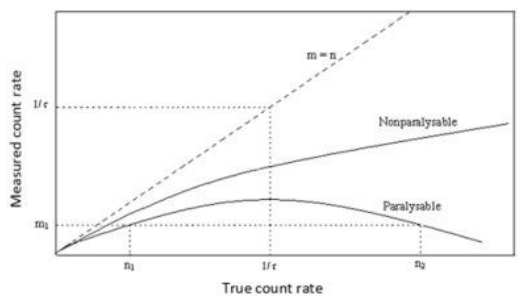
\includegraphics[width=8cm]{morto1.png}
    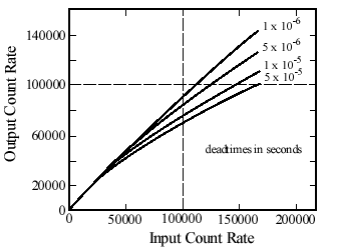
\includegraphics[width=8cm]{morto2.png}
\end{center}

\section{Stima del tempo morto}
Molto spesso il tempo morto di un sistema di conteggio non è noto esattamente. Esistono vari metodi per stimarne il valore. Uno di questi è il cosiddetto “\textit{metodo delle due sorgenti}”. 
\begin{center}
    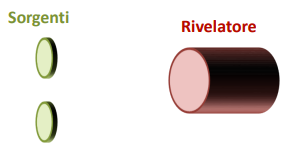
\includegraphics[width=4cm]{mortostima.png}
\end{center}
Misurando il rate $R_1$ ed $R_2$ delle due sorgenti separatamente e il rate
$R_{12}$ delle due sorgenti insieme in assenza di fondo è possibile stimare il
tempo morto $\tau$:
$$\tau=\frac{R_1R_2-\sqrt{R_1R_2(R_{12}-R_1)(R_{12}-R_2)}}{R_1R_2R_{12}}$$

\section{Funzioni di un rivelatore}
Un rivelatore di particelle può servire a misurare:
\begin{itemize}
    \item energia;
    \item impulso;
    \item carica;
    \item massa;
    \item tempo di arrivo.
\end{itemize}
I grandi rilevatori per la fisica nucleare e particellare comprendono diverse componenti (sotto-rivelatori) per il tracciamento e l'identificazione delle numerose (anche decine di migliaia) particelle prodotte in una singola collisione.\\
L'\textit{energia} misurata mediante un rivelatore corrisponde all'energia in esso depositata quindi non necessariamente questa corrisponde con l'energia iniziale della particella o della radiazione. I rilevatori che assorbono totalmente l'energia di una particella o di un radiazione vengono detti
“\textit{calorimetri}”. Un particolare esempio di calorimetri sono quelli adronici, utilizzati nella fisica ad alta energia per misurare l'energia di una cascata adronica (ad alte energie, l'impulso è in pratica una
misura dell'energia).\\
L'\textit{impulso} di una particella carica è di solito misurato mediante un opportuno campo magnetico che ne deflette la traiettoria. Nella fisica nucleare di bassa energia si utilizzano opportuni spettrometri magnetici, esistenti sotto varie configurazioni. In genere l’uso di spettrometri magnetici consente una risoluzione in impulso estremamente elevata.\\
Un esempio di dipolo magnetico, usato per deflettere una particella carica e misurarne l’impulso dalla curvatura della traccia può essere del tipo:
\begin{center}
    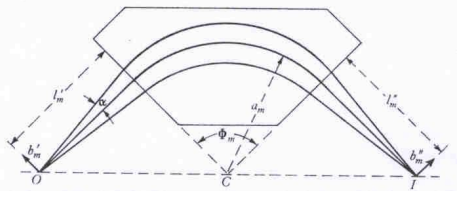
\includegraphics[width=6cm]{riv_ese2.png}
\end{center}
Un altro esempio di magnete, usato per deflettere le particelle cariche prodotte in una reazione nucleare può essere:
\begin{center}
    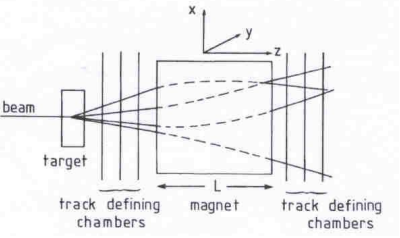
\includegraphics[width=6cm]{riv_ese1.png}
\end{center}
Una particella, inoltre, può essere identificata misurando il rapporto massa su carica oppure mediante la formula di Bethe-Bloch misurando la perdita di energia in funzione dell'energia stessa.
Le principali categorie di rivelatori sono quelli a gas, quelli a semiconduttore e gli scintillatori.\\
Il segno della carica di una particella può essere stabilito tramite la curvature che la particella assume in un campo magnetico.\\
Nella fisica nucleare di bassa energia, la carica di una particella (p, He, Li,…) può essere misurata mediante la perdita di energia (tecnica $\Delta E-E$) in un telescopio.

\section{ALICE: un rivelatore complesso}
Acronimo di: \textbf{A Large Ion Collider Experiment}, è un rivelatore costruito per \textbf{LHC}. Tale rivelatore ha lo scopo di studiare le particelle prodotte (adroni, elettroni, muoni e fotoni) a seguito di urti tra nuclei di piombo oppure collissioni protone-protone.\\ 
Tale rivelatore permette il tracciamento di particelle cariche. La curvatura di una particella in un campo magnetico permette di stabilire il segno della carica (+/-).
\begin{figure}[h!]
    \centering
    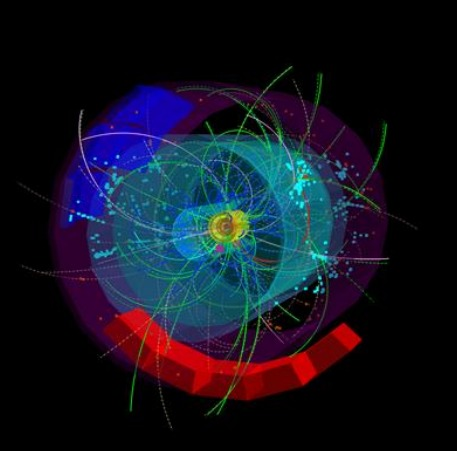
\includegraphics[scale=0.5]{ALICE_RIV.jpeg}
    \caption{Traiettoria curvata delle particelle cariche}
    \label{fig:enter-label}
\end{figure} 
\newpage
L' acquisizione di tutti i dati utili è effettuata tramite l'utilizzo di 18 sotto rivelatori che utilizzano tecnologie differenti:
\begin{itemize} % Rimosso [h!] che era fuori dal \begin{figure}

    \item \textbf{Inner Tracking System}: 7 strati concentrici cilindrici di pixel monolitici progettati per le elevate densità di particelle vicino al punto di interazione tra i fasc; per un totale di 10 $m^2$
    \item \textbf{Time Of Flight}: Multi-gap Resistive Plate Chambers, i quali ricoprono un area di 150 $m^2$ aventi una risoluzione temporale 90 ps, efficienza $\approx$ 95\%.
    
    \item \textbf{High Momentum Particle Identification}: Ring      Imaging, composto da 7 moduli per un totale di 12 $m^2$
    
    \item \textbf{Di-muon spectromete}:Permesso tramite l'utilizzo di 10 piani di tracciamento aventi 4 RPC per trigger.

    \item \textbf{Zero Degree Calorimeters}: 2 coppie di calorimetri sampling per rivelare i protoni e i neutroni spettatori a 115 m dal punto d’interazione.

    \item \textbf{EMCal $\rightarrow$ Electromagnetic Calorimeter}: 11 super-moduli, 44 $m^2$ tecnologia sampling Pb-scintillatore. 
    
\end{itemize}

L'analisi dati è effettuata tramite \textit{GRID} e strutture di calcolo. \\

\section{Sala controllo ALICE}
Tutti gli esperimenti LHC prendono dati durante la maggior parte dell'anno. Monitorare la qualità dei dati durante il corso dell'esperimento è un compito di fondamentale importanza. \\
Considerando una media di 600 milioni di collisioni al secondo prodotte dalle interazione tra i fasci. I trigger di selezione degli eventi riducono il numero degli eventi di interessa a qualche KHz.
 Ma in ogni caso tali eventi comportano un flusso dati di diversi Gbytes/s, in quanto ogni evento è nell'ordine di 1 Mbyte. \\ 
 

\chapter{Rivelatori a gas}
Questi dispositivi sono stati i primi ad essere utilizzati per la rivelazione di particelle. Essi sfruttano la \textit{ionizzazione} prodotta dal passaggio di un fotone o di una particella carica in un gas; in tale processo un elettrone viene rimosso da un atomo o da una molecola in modo da creare una coppia elettrone-ione positivo.
\begin{center}
    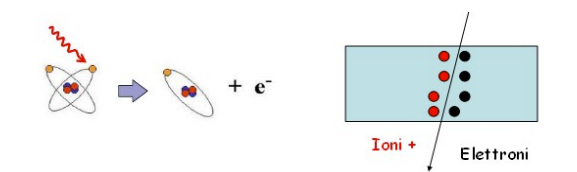
\includegraphics[width=10cm]{rivgas.png}
\end{center}
Possono essere usati in:
\begin{itemize}
    \item Current mode;
    \item Pulsed mode.
\end{itemize}
Se una radiazione penetra nel rivelatore sarà creato un certo numero di coppie ione-elettrone, sia direttamente, se la radiazione è una particella carica, che indirettamente attraverso radiazioni secondarie, se la radiazione è neutra.\\
Il numero medio di coppie create è proporzionale all'energia depositata nel dispositivo. 

\section{Ionizzazione}
La perdita di energia di una particella carica nella materia è essenzialmente suddivisa tra due tipi di reazione:
\begin{itemize}
    \item eccitazione $\rightarrow$ risonanza;
\item ionizzazione $\rightarrow$ soglia.
\end{itemize}
in cui vengono creati un elettrone e uno ione liberi.\\ 
L'eccitazione di un atomo, X,
$$X+p\longrightarrow X^*+p$$
dove $p$ è una particella carica, è una reazione risonante che richiede la quantità corretta di energia da trasferire. Le sezioni d'urto tipiche nei gas nobili alla risonanza sono
dell'ordine di $\sigma\simeq 10^{-17}cm^2$. Sebbene non vengano creati elettroni o ioni liberi, la molecola o l'atomo eccitato può partecipare a ulteriori reazioni che provocano la ionizzazione.
Questo è discusso in seguito.\\
Per una ionizzazione,
$$X+p\longrightarrow X^++p+e^-$$
non c'è, ovviamente, un fabbisogno energetico esatto e, infatti, la sua sezione trasversale è un po' più alta con $\sigma\simeq 10^{-16}cm^2$.\\ 
Tuttavia, il processo di ionizzazione ha una soglia di energia che è relativamente alta, e poiché sono più probabili trasferimenti a bassa energia, le reazioni di eccitazione generalmente dominano.\\
Ciò che è sorprendente è che il numero di coppie dipende più che dal tipo di radiazione ionizzante dal tipo di gas. 
Nella tabella sottostante vi sono alcuni valori di $w$, energia media richiesta per creare una coppia elettrone-ione.
\begin{center}
    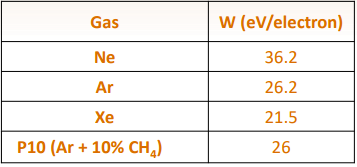
\includegraphics[width=6cm]{wvalore.png}
\end{center}
Per ottenere il numero di coppie formate occorre dividere l'energia persa $E$ per $w$:
$$N=\frac{E}{w}$$
In questo modo tenendo conto, se necessario, del fattore di Fano, F, può essere calcolata la risoluzione energetica del rivelatore:
$$R=2.35\sqrt{\frac{Fw}{E}}$$
In generale la risoluzione in energia è funzione dell'energia depositata o per ionizzazione o per eccitazione delle molecole del mezzo. Esistono delle fluttuazioni nel numero di coppie formate da particelle ionizzante, incidenti con la stessa energia. Tali fluttuazioni pongono un limite alla risoluzione energetica che può essere raggiunta in un rilevatore e variano quando la radiazione viene completamente o in parte assorbita dal mezzo.
Per un rilevatore che assorbe solo una parte dell'energia della particella la formazione di ciascuna coppia di ioni può essere considerata un processo Poissoniano; in questo caso la risoluzione del rilevatore dovrebbe essere:
$$R=\frac{2.35}{\sqrt{N}}$$
dove $N$ è il numero di coppie formate.\\
Le misure sperimentali della risoluzione hanno mostrato che questa risulta più piccola del predetto valore nel caso in cui la particella all'interno del rivelatore perda tutta la propria energia. In questo caso, dunque, l'energia depositata costituisce un valore fissato e la ionizzazione dipenderà direttamente da tale valore. Statisticamente, ciò si traduce nel fatto che i vari processi di ionizzazione non sono del tutto indipendenti e pertanto la statistica di Poisson non risulta più applicabile. A tale proposito è stato introdotto il fattore di Fano che tiene conto della frazione di energia della particella incidente che non è convertita in informazione rivelabile. La risoluzione del rivelatore tenendo conto del fattore di Fano, $F$, risulta:
$$R=2.35\sqrt{\frac{F}{N}}$$
Nel caso in cui il modello Poissoniano è valido tale fattore ha valore 1, in realtà il suo valore è sempre minore di 1.\\
Gli elettroni e gli ioni creati dalla radiazione incidente stessa sono noti come \textit{ionizzazione primaria}. In un certo numero di queste ionizzazioni, tuttavia, una quantità sufficientemente grande di energia viene trasferita all'elettrone (raggi delta) in modo tale che questo elettrone crei anche coppie ione-elettrone. Quest'ultima ionizzazione è nota come \textit{ionizzazione secondaria}. Se la loro energia è sufficientemente elevata, anche gli elettroni di ionizzazione secondaria possono ionizzarsi e così via fino al raggiungimento della soglia per le reazioni di ionizzazione.\\
Per creare una coppia di ioni sono necessari circa $25- 40 eV$. Questo valore può dipendere dall'energia per nucleone del fascio incidente.
\begin{center}
    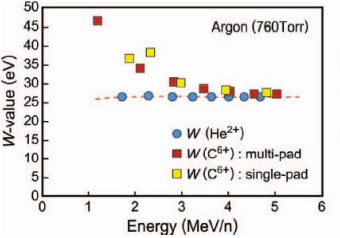
\includegraphics[width=6cm]{wvalore1.png}
\end{center}
Ovviamente queste misure sono soggette a fluttuazioni statistiche.\\
Supponendo che nel caso ideale l'energia depositata sia uguale a quella totale, ovvero che tutte le particelle si fermino nel rilevatore depositando tutta la loro energia, le fluttuazioni statistiche sono,
ovviamente, nulle.\\
Per un fenomeno che segue la statistica di Poisson, invece, le fluttuazioni sono dell'ordine di
$$\sigma=\sqrt{N}$$
Mentre nel caso in cui il fenomeno non segua la statistica di Poisson, le fluttuazioni sono dell'ordine:
$$\sigma=\sqrt{FN}$$
dove $N$, in entrambi i casi, è il numero di coppie.\\
Nella tabella sottostante vi sono valori del fattore Fano per i gas nobili.
\begin{center}
    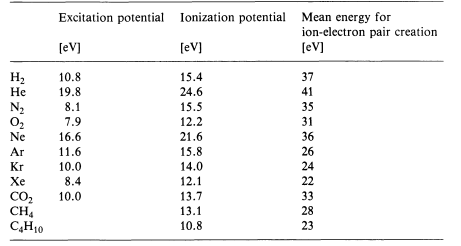
\includegraphics[width=10cm]{fanonobili.png}
\end{center}

\section{Diffusione, Ricombinazione e Migrazione}
Le cariche, una volta prodotte, possono:
\begin{itemize}
    \item diffondersi;
    \item ricombinarsi;
    \item migrare.
\end{itemize}

\section{Diffusione}
Il diffondersi delle particelle è un fenomeno che si verifica solo in assenza di campi elettrici. Gli elettroni e gli ioni liberati dal passaggio della radiazione si diffondono uniformemente verso l'esterno dal loro punto di creazione. Nel processo subiscono collisioni multiple con le molecole del gas e perdono la loro energia. Entrano così rapidamente in equilibrio termico con il gas e alla fine si ricombinano. 
Le velocità delle cariche sono descritte dalla distribuzione di Maxwell, esse hanno una velocità media proporzionale a 
$$\sqrt{\frac{kT}{m}}$$
Ovviamente, la velocità media degli elettroni è molto maggiore di quella degli ioni a causa della loro massa minore. A temperatura ambiente, la velocità dell'elettrone è di circa $10^6 cm/s$ mentre le velocità degli ioni positivi sono dell'ordine di $10^4 cm/s$.\\
La distribuzione delle distanze percorse, a un tempo $t$, è:
$$\frac{dN}{dx}=\frac{N_0}{\sqrt{4\pi D t}}e^{-\frac{x^2}{4Dt}}$$
con
$$\sigma=\sqrt{6Dt}$$
$$D=\frac{2}{3\sqrt{\pi}}\frac{1}{p\sigma_0}\sqrt{\frac{(kT)^3}{m}}$$
dove $D$ è il coefficiente di diffusione, $p$ la pressione e $\sigma_0$ è la sezione d'urto di interazione.

\section{Ricombinazione}
La \textit{ricombinazione} risulta essere il processo mediante il quale a causa delle collisioni fra ioni positivi ed elettroni liberi, questi ultimi possono essere catturati dai primi con il conseguente ritorno allo stato di neutralità. Alternativamente potrebbe avvenire una collisione fra ione positivo e ione negativo, che cede l'elettrone extra al primo con la conseguente neutralizzazione di entrambi gli ioni. In ogni caso viene persa l'informazione sulla ionizzazione prodotta all'interno del rivelatore.\\ 
Poiché la frequenza di collisione è proporzionale al prodotto della concentrazione delle due specie coinvolte, il rate di ricombinazione è dato:
$$\frac{dn^+}{dt}=\frac{dn^-}{dt}=-\beta n^+n^-$$
dove $n^+$ è la densità numerica degli ioni positivi, $n^-$ è la densità degli ioni negativi e $\beta$ è il coefficiente di ricombinazione.\\
Il coefficiente di ricombinazione fra ioni positivi e negativi è solitamente parecchi ordini di grandezza più grande di quello fra ioni positivi ed elettroni.
La ricombinazione può essere, quindi, essenzialmente di due tipologie:
\begin{itemize}
    \item Ricombinazione di ioni positivi con elettroni o con ioni negativi:
    $$X^++e^-\rightarrow X+h\nu$$
    $$X^++Y^-\rightarrow XY+e^-$$
    \item Ricombinazione di elettroni con ioni positivi o molecole elettronegative:
    $$e^-+X^+\rightarrow X+h\nu$$
    $$e^-+X\rightarrow X^-+h\nu$$
\end{itemize}
Per essere rivelati, elettroni e ioni positivi devono sopravvivere per un tempo almeno pari al tempo di raccolta degli elettroni, in altre parole, affinchè le particelle vengano rivelate il tempo di risposta dello strumento deve essere minore del tempo di ricombinazione. Per tale ragione spesso la scelta del gas verte su quelli costituiti da molecole non molto elettronegative.\\
Alcuni gas elettronegativi hanno tempi di attaccamento molto brevi, ad esempio per $O_2$ è di $140 ns$.

\section{Migrazione}
La migrazione si ha, infine, sotto l'azione di un campo elettrico che porta ad uno spostamento di cariche con una velocità di drift sovrapposta al moto casuale dovuto all'agitazione termica.\\ 
La velocità di drift è data da:
$$V_{drift}=\mu\frac{E}{p}$$
dove $E$ è il campo elettrico, $p$ la pressione e $\mu$ è la \textit{mobilità} espressa in $\frac{m^2 atm}{V s}$.
Rispetto alle loro velocità termiche, la velocità di drift degli ioni è minore rispetto a quella degli elettroni, può essere molto più elevata poiché sono molto più leggeri.\\
Le velocità di drift possono essere accuratamente misurate e calcolate per gas specifici, per valutare la risposta dettagliata di un rivelatore
\begin{center}
    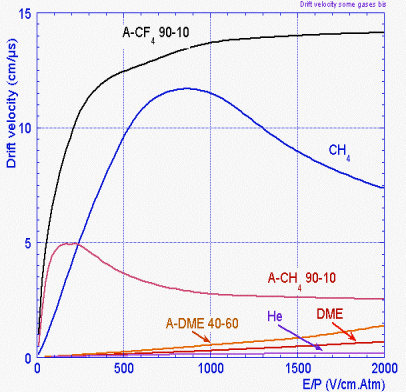
\includegraphics[width=8cm]{deriva_vel.png}
\end{center}
Per piccoli valori di $E/p$ la velocità è proporzionale a questa quantità a $\mu$.

\section{Principio di funzionamento del rivelatore a gas}
Lo schema di principio di un rivelatore a gas include un recipiente a tenuta di gas all'interno del quale vi sono due elettrodi, ad esempio un condensatore piano, e una differenza di potenziale.
\begin{center}
    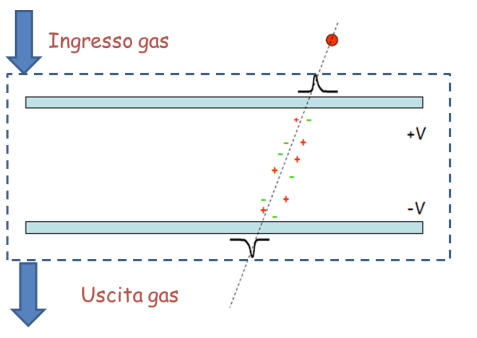
\includegraphics[width=8cm]{gas_riv1.png}
\end{center}
Le particelle ionizzate si muovono lungo la direzione del campo elettrico depositandosi sugli elettrodi. A causa, però, sia dell'interazione con i raggi cosmici e con le sorgenti radioattive che della ionizzazione, un dispositivo di questo tipo è soggetto a scaricarsi velocemente. \'E necessario per cui collegarlo ad un generatore di corrente continua e ad un resistenza.
\begin{center}
    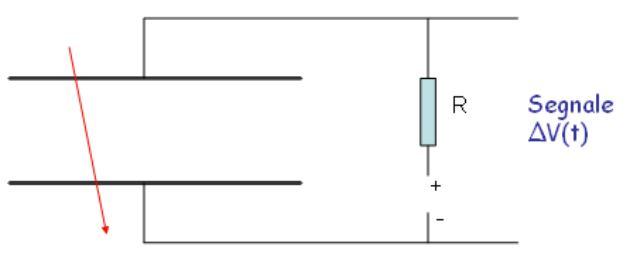
\includegraphics[width=8cm]{gas_riv2.png}
\end{center}
Per rispondere ad impulsi singoli il rivelatore (condensatore) deve essere polarizzato mediante una resistenza R di valore molto elevato ovvero dell'ordine di $10^7-10^8 \Omega$.\\
Se $V_0$ è la tensione di alimentazione, quando sul rivelatore giungono le particelle cariche (ioni o elettroni) la tensione sulle armature diminuisce sino al valore di $V_0-neC$, per poi ritornare nuovamente al valore di $V_0$ seguendo la legge di carica esponenziale (costante di tempo $RC$).
\begin{center}
    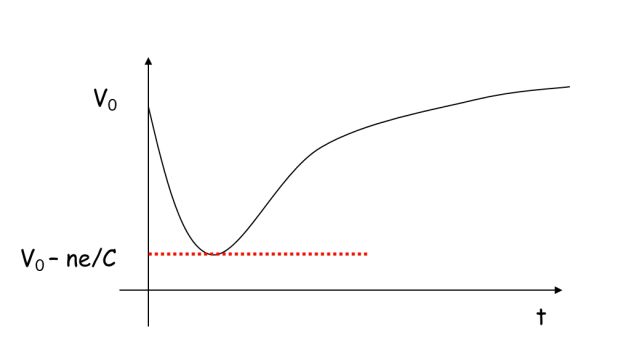
\includegraphics[width=8cm]{gas_riv3.png}
\end{center}
volendo essere più precisi, il segnale di tensione dipende della distanza $x$ tra le armature e il punto dove avviene la ionizzazione. Per ovviare a questo problema si può utilizzare una griglia posta tra le due armature, detta \textit{griglia di Frisch}, che modifica il campo elettrico in modo da rendere indipendente la tensione dalla distanza di griglia $x$.\\
La griglia scherma l'anodo dall'induzione degli ioni positivi. L'anodo misura così un segnale legato solo agli elettroni e indipendente dalla posizione della traccia.
\begin{center}
    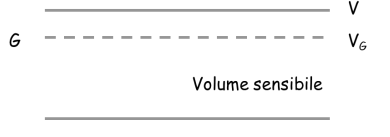
\includegraphics[width=8cm]{gas_riv7.png}
\end{center}
L'impulso di tensione è la somma di due componenti: una dovuta agli elettroni e una dovuta agli ioni positivi.\\
La forma della curva dipende dalla costante di tempo $RC$
\begin{center}
    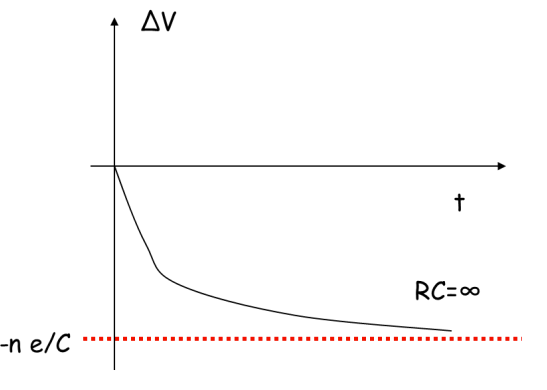
\includegraphics[width=8cm]{gas_riv4.png}
\end{center}
Se, ad esempio, si adopera una costante di tempo intermedia tra il tempo di raccolta degli elettroni e quello degli ioni positivi, si avrà un impulso più veloce ma di ampiezza minore.
\begin{center}
    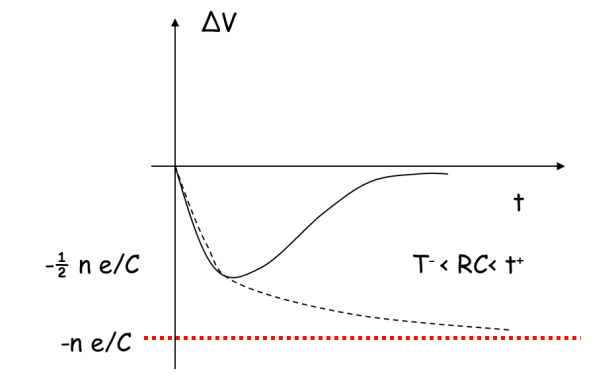
\includegraphics[width=8cm]{gas_riv5.png}
\end{center}
Tale impulso dipende inoltre dalla posizione della traccia nel volume sensibile:
\begin{center}
    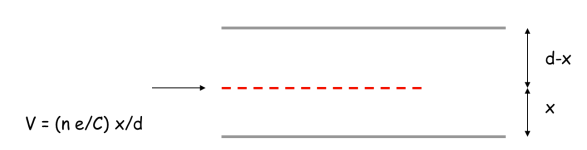
\includegraphics[width=10cm]{gas_riv6.png}
\end{center}
Si possono adoperare costanti di tempo $RC<t$. In questo caso l'ampiezza dell'impulso è
proporzionale a $n\frac{e}{C}$ ma è molto piccola.

\section{Moltiplicazione}
La moltiplicazione in un rilevatore a gas avviene quando gli elettroni provenienti da ionizzazione primaria accelerati dal campo elettrico riescono a ionizzare le molecole del gas. Gli elettroni secondari possono produrre una nuova ionizzazione e così via, con la formazione di una valanga di ioni, conosciuta con il nome di \textit{valanga Townsend}.\\
I gas nobili possono essere eccitati e diseccitati solo attraverso assorbimento ed emissione di fotoni. Mentre per quanto concerne le molecole di gas poliatomici debolmente legati, queste posso eccitarsi o diseccitarsi attraverso moti rotazionali e vibrazionali senza emissione di fotoni. \\
%La probabilità di ionizzazione secondaria aumenta con l'energia degli elettroni ed ha il suo massimo a circa $100 eV$.\\
Innanzitutto è necessario premettere che il \textit{libero cammino medio per ionizzazione} $\lambda$ è definito come la distanza media tra due collisioni che provocano ionizzazione ed il suo inverso $\alpha$, noto come \textit{primo coefficiente di Towsend}, rappresenta il numero di coppie ioniche prodotte per unità di cammino:
$$\alpha=\frac{1}{\lambda}$$
Premesso ciò, data una distanza $\lambda$, l'elettrone ionizza e libera una coppia elettrone-ione. I due elettroni proseguono il loro cammino e a loro volta ionizzano e così via. Causando un processo di moltiplicazione a $valanga$.\\
Indichiamo con $M$ il \textit{fattore di moltiplicazione o guadagno}:
$$M=\frac{n}{n_0}=e^{\alpha x}$$
dove $n$ è il numero totale di elettroni creati nel processo x, $n_0$ è il numero di elettroni prodotti per ionizzazione primaria e $\alpha$ è il coefficiente di Townsend. Fisicamente, il fattore di moltiplicazione è limitato a circa $M < 10^8$ dopodiché si verifica la \textit{rottura}. Questo è noto come il \textit{limite di Raether}.\\
A causa della grande mobilità degli elettroni rispetto agli ioni positivi, la valanga ha la forma di una \textit{goccia di liquido} con gli elettroni raggruppati in testa e gli ioni più lenti in coda.
\begin{center}
    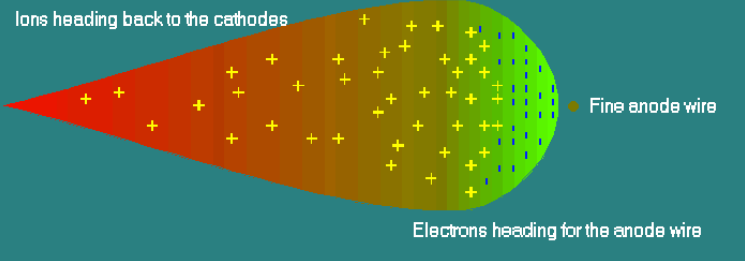
\includegraphics[width=8cm]{valanga.png}
\end{center}
Quando si hanno $n$ elettroni primari, la frazione di elettroni secondari formati per unità di percorso è governata dall'equazione di Townsend: $dn=n\alpha dx$.\\
Integrando in un percorso x si ottiene:
$$n=n_0 e^{\alpha x}$$
dove $n_0$ è il numero iniziale di elettroni.

\newpage
\section{Regimi di lavoro dei rivelatori a gas}
A seconda del campo elettrico un rivelatore può lavorare in vari regimi, assumendo nomi differenti.
\begin{center}
    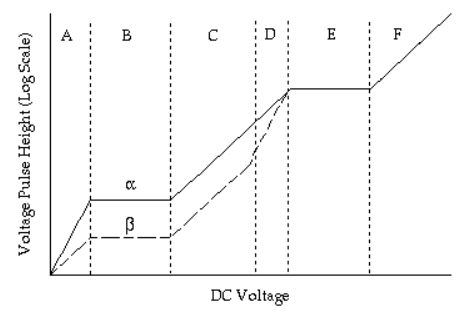
\includegraphics[width=8cm]{gas_regimi.png}
\end{center}
Nella regione A non tutte le cariche prodotte vengono raccolte in quanto, a causa del piccolo valore del campo elettrico, il processo di ricombinazione delle varie coppie ione-elettrone è notevole.
Aumentando la differenza di potenziale applicata il tempo a disposizione per la ricombinazione diminuisce, perché aumenta la componente della velocità delle coppie lungo la direzione del campo; questo crea un aumento della carica raccolta.\\
Nella regione B, chiamata di saturazione o di camera a ionizzazione, gli effetti della ricombinazione diventano trascurabili e la carica raccolta è tutta quella prodotta.
Nelle regioni C e D il campo elettrico è sufficientemente intenso da far acquistare agli elettroni primari prodotti energia cinetica sufficiente a ionizzare gli atomi del gas producendo, così, una moltiplicazione a valanga di ioni. La ionizzazione secondaria è ancora strettamente dipendente da quella primaria ed è in questa regione che lavorano i contatori proporzionali.\\
Nella regione E, detta di Geiger-Muller, la carica raccolta non è più proporzionale alla ionizzazione primaria;  oltre alla ionizzazione si hanno altri fenomeni quali l'eccitazione seguita da emissione di luce visibile e ultravioletta; questo produce un impulso costante in un certo intervallo del potenziale applicato, indipendentemente dal tipo di particella incidente.\\
Nella regione F non è più possibile nessun tipo di rivelazione: l'impulso in uscita non dipende più dalla radiazione incidente, poiché avviene una scarica in presenza o meno di radiazione.

\section{Geometrie dei rivelatori a gas}
Per un rivelatore a gas sono possibili diverse configurazioni a seconda delle dimensioni, del regime in cui i rilevatori devono operare e delle performance richieste.\\
Esistono due possibili configurazioni base:
\begin{itemize}
    \item una planare (equivalente ad un condensatore a facce piane e parallele);
    \item una cilindrica (equivalente ad un condensatore cilindrico);
\end{itemize}
\begin{center}
    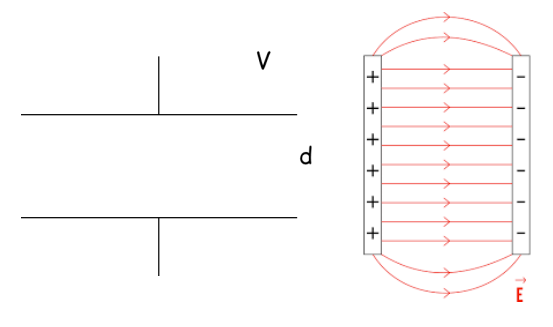
\includegraphics[width=7cm]{gas_piano.png}
    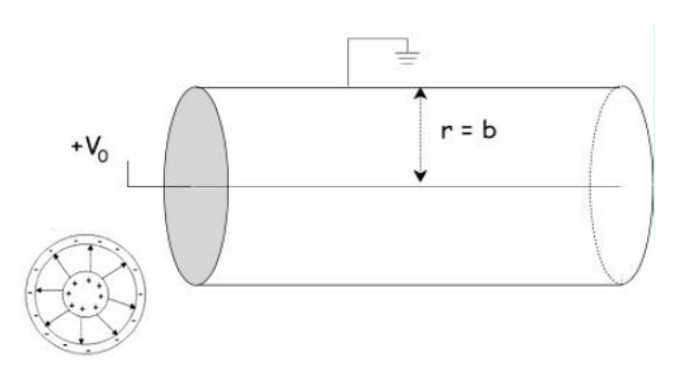
\includegraphics[width=7cm]{gas_cilindro.png}
\end{center}
Le due si differenziano principalmente per i diversi andamenti dei campi elettrici al loro interno.\\
Per una \textit{struttura planare} in cui la differenza di potenziale fra piano-catodo e piano-anodo è $V_0$, il modulo delle linee di campo vale:
$$E=\frac{V_0}{d}$$
dove $d$ è la distanza fra i due piani.
La \textit{configurazione cilindrica} è costituita da un cilindro cavo, che funge da catodo, al cui interno è contenuto un filo conduttore, mantenuto ad un potenziale $V_0$ rispetto al cilindro. Il campo elettrico radiale che si viene a formare all'interno del rivelatore ha un modulo pari a:
$$E(r)=\frac{V_0}{r\ln(\frac{b}{a})}$$
dove $r$ è la distanza radiale dal filo conduttore, $b$ è il raggio interno del cilindro e $a$ il raggio del filo conduttore.


\section{Contatore Geiger}
Un \textit{contatore Geiger-Muller} è composto da un catodo cilindrico di $1-10 cm$ di diametro con una lunghezza che è da due a dieci volte maggiore.  Esso opera nella regione E della curva segnale d'uscita-potenziale in un rivelatore a gas.\\
In questi dispositivi la carica raccolta è indipendente dalla ionizzazione primaria. Infatti oltre alla ionizzazione si hanno fenomeni quali l'eccitazione seguita da emissione di luce visibile e ultravioletta. Una piccola parte di tali fotoni dà luogo ad emissione di fotoelettroni che generano nuova ionizzazione, tramite il processo della moltiplicazione a valanga.\\
Nella regione di funzionamento di un contatore Geiger-Muller basta una sola coppia primaria per dar luogo ad una scarica a valanga completa e, quindi, l'ampiezza dell'impulso in uscita non è più una misura della ionizzazione primaria. Da ciò si comprende che un contatore Geiger può essere utilizzato come contatore di radiazione e non in esperimenti di spettroscopia.
\begin{center}
    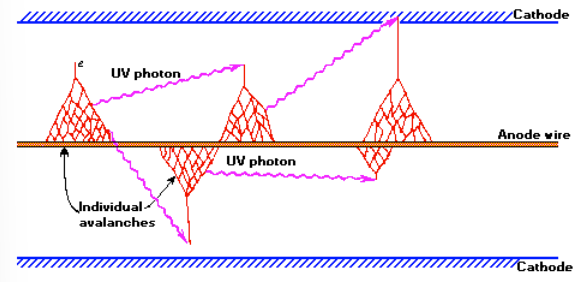
\includegraphics[width=8cm]{geiger1.png}
\end{center}
Un grafico ottenuto riportando in ascisse le tensioni applicate, ed in ordinate il numero degli impulsi registrati in un intervallo di tempo T (uguale naturalmente per tutte le misure) si chiama "\textit{curva caratteristica del contatore}" ed ha l'andamento mostrato nella figura sottostante:
\begin{center}
    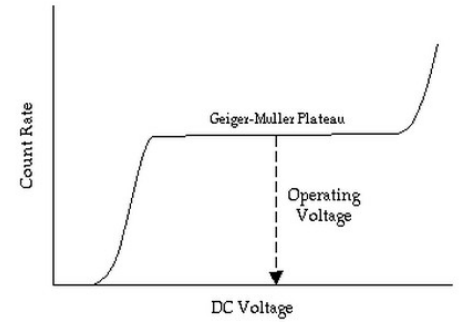
\includegraphics[width=8cm]{geiger2.png}
\end{center}
Tale curva presenta una zona lunga centinaia di Volt a piccola pendenza che viene chiamata "\textit{pianerottolo}" del contatore.\\
La tensione di lavoro del contatore viene scelta a circa $1/3$ di tutto il pianerottolo, in modo che eventuali variazioni nella tensione di alimentazione $V$ del contatore non lo portino al di fuori della regione di lavoro; d'altra parte, l'applicazione di una tensione più alta può produrre cariche spurie all'interno del rivelatore.\\
In base alla geometria essi possono funzionare come rivelatori di raggi $\beta$, $\gamma$ o $X$.
I contatori per raggi $\beta$ devono poter offrire un piccolissimo assorbimento agli elettroni e per tale motivo una parte del tubo viene provvista di una finestra ricoperta da un materiale molto sottile, di bassa densità e di resistenza meccanica sufficiente a sopportare la differenza tra pressione interna ed esterna. L'efficienza intrinseca risulta del $100\%$.\\
I contatori per raggi $\gamma$ funzionano a causa della ionizzazione dovuta agli elettroni prodotti per effetto fotoelettrico, per effetto Compton o per creazione di coppie dall'interazione dei raggi $\gamma$ con le pareti o con il gas di riempimento. A causa della bassa probabilità di interazione con il gas, occorre affidarsi all'interazione con le pareti e utilizzare contatori senza finestra e con spessori notevoli delle pareti metalliche. Con tutto ciò l'efficienza intrinseca risulta quasi bassa.\\
I contatori per raggi $X$ sono simili a quelli per raggi $\beta$. Infatti poiché i raggi $X$ sono fotoni con energie più basse dei raggi $\gamma$, occorrono contatori con pareti sottili e con finestra di mica, in modo che l'interazione avvenga con le molecole del gas. Generalmente i gas impiegati sono l'argon, il krypton e lo xenon. Generalmente sono usate le \textit{camere proporzionali} per la rivelazione dei raggi $X$, in particolare per quelli a bassa energia dell'ordine di pochi $KeV$ e di elettroni di bassissima energia. Di solito i gas utilizzati sono mantenuti
a pressione atmosferica, ma possono essere utilizzate pressioni più alte per poter accrescere la densità e quindi l'efficienza del rivelatore.\\
I rivelatori Geiger-Müller possono avere anche altri impieghi come ad esempio la misura del coefficiente di assorbimento per raggi $\alpha$ o $\beta$ nell'attraversare un mezzo materiale. Ciò può essere ottenuto misurando il numero di conteggi in un tempo fissato in assenza di materiale e vedendo come questo varia interponendo fra sorgente e contatore il materiale di volta in volta con spessori diversi.

\section{Rivelatori a gas moderni}
A parte i contatori Geiger, ancora adoperati in piccoli sistemi di rivelazione o per uso didattico, camere a ionizzazione e contatori proporzionali sono usate di rado o solo per specifiche applicazioni (ad esempio in campo medico).\\
Esistono tuttavia molte versioni “moderne” di rivelatori a gas, usate anche negli attuali esperimenti di fisica nucleare e astro-particellare.

\section{Camere a fili o MWPC ( Multiwire Proportional Chambers)}
Ideato nel 1968 al CERN da Georges Charpak, ha valso al suo inventore il Premio Nobel per la fisica nel 1992.\\
Le camere a fili sono ottenute includendo nello stesso volume gassoso più camere proporzionali, costituite da una serie di fili sottili, con raggio di circa $20\mu m$, che fungono da anodo spaziati circa $2$ mm l'uno dall'altro e distanti circa $7-8$ mm dalle pareti piane, che costituiscono il catodo.
\begin{center}
    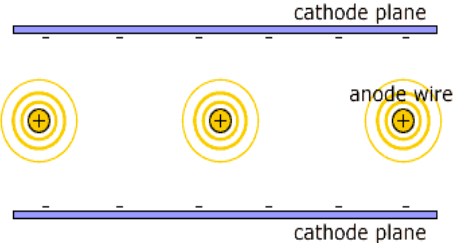
\includegraphics[width=8cm]{riv_filo2.png}
\end{center}
Se ai piani-catodo viene applicato un voltaggio negativo, la distribuzione delle linee di campo elettrico risultano parallele lungo tutto il rivelatore eccetto che nella regione vicino ai fili, dove il campo ha una dipendenza 1/r simile a quella che si ottiene in una camera proporzionale cilindrica con un singolo filo. Esistono specifici programmi di calcolo delle linee di campo, in quanto la loro conoscenza permette, specie in prossimità dei fili, una valutazione delle prestazioni del rivelatore.
\begin{center}
    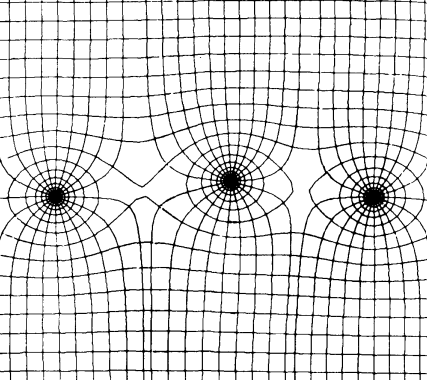
\includegraphics[width=6cm]{riv_filo.png}
\end{center}
Se in una MWPC una coppia ione-elettrone viene formata nella regione dove si ha il campo elettrico costante i vari ioni deriveranno lungo la direzione del campo, in modo tale che gli elettroni si avvicineranno al filo più vicino e gli ioni ai piani-catodi. Se ciascun filo ha un diametro di circa $20\mu m$ nelle sue vicinanze sarà prodotto un campo elettrico intenso, che può far accelerare gli elettroni fino a produrre una valanga. Gli ioni positivi liberati nel processo di moltiplicazione inducono un segnale negativo sul filo-anodo più vicino ed influenzano anche i fili confinanti dove però verrà prodotto un segnale positivo di piccola ampiezza. Viceversa gli elettroni indurranno un segnale positivo sui piani-catodo. In tale maniera si elimina l'ambiguità su quale sia il filo più vicino all'evento ionizzante e ciò permette di rivelare una coordinata della posizione. La seconda coordinata può essere ottenuta utilizzando un altro rivelatore in i fili-anodo sono disposti perpendicolarmente ai primi.\\
Una misura della traiettoria della particella può essere ottenuta allineando due o più MWPC in modo da ottenere una ricostruzione della traccia guardando i fili che hanno fornito il segnale.

\section{Camere a drift}
Le \textit{camerea drift} sono delle versioni delle MWPC con lettura del tempo di drift in ogni filo. Consente risoluzioni migliori, ma richiede un’elettronica più complessa.
\begin{center}
    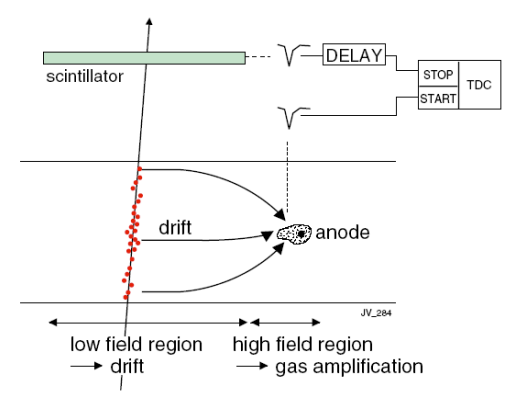
\includegraphics[width=8cm]{riv_drift.png}
\end{center}

\section{TPC: Time Projection Chamber}
Uno dei più sofisticati rivelatori a ionizzazione è la Time Projection Chamber o TPC. Questo dispositivo è un rivelatore di tracce tridimensionale capace di fornire informazioni su diversi punti della traccia della particella insieme ad informazioni sulla perdita specifica di energia, $dE/dx$. Essa è molto utilizzata nella fisica delle alte energie.\\
Permette di misurare la coordinata $z$ (assiale) dal tempo di drift e le coordinate $(x,y)$  dalla particolare pad che raccoglie il segnale.
\begin{center}
    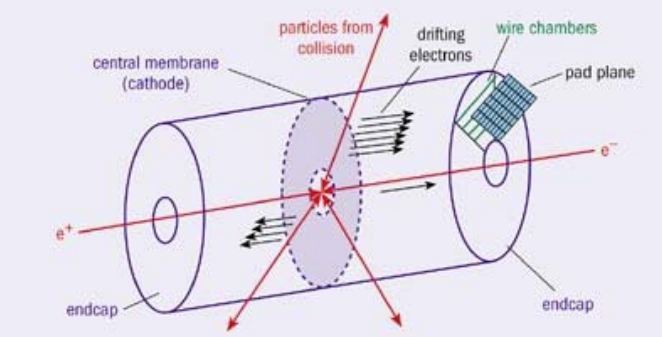
\includegraphics[width=8cm]{riv_tpc1.png}
\end{center}
La TCP dell'esperimento ALICE@LHC è la più grande costruita finora.
\begin{center}
    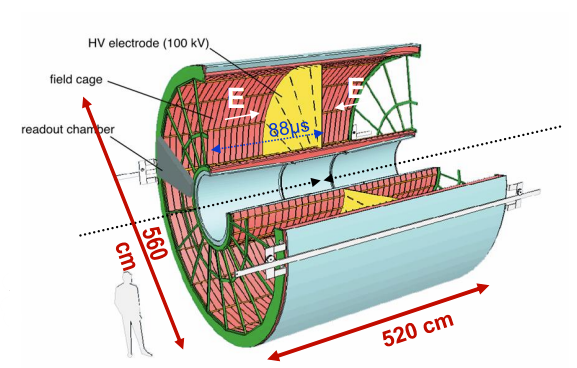
\includegraphics[width=8cm]{riv_tpc.png}
\end{center}

\section{MRPC: Multigap Resistive Plate Chambers}
\begin{figure}[H]
    \centering
    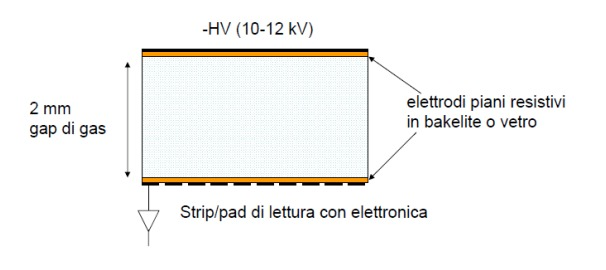
\includegraphics [width= 8 cm]{MRPC.jpeg}
    \caption{Resistive Plate Chambers}
    \label{fig:mrpc}
\end{figure}
Dunque in base al gap si possono ottere diverse caratteristiche del rivelatore in questione:
\begin{itemize}
    \item Gap piccola: ridotte fluttuazioni di guadagno, ridotte scariche, ridotte fluttuazioni di posizione di 
    rilascio ionizzazione ($\Delta\tau$ piccolo).
La distanza tra le due placche per questi rivelatore è pari a $D_{gap} \approx 200-300 \mu m$; con miscele di gas dense/veloci. \\
    \item Multi-gap: piena efficienza.
    \item  Miscele di gas dense/veloci: $\Delta\tau$ piccolo.
\end{itemize}
Tali rivelatori all'avanguardia si trovano in due esperimenti attualmente:
\begin{itemize}
    \item Rivelatori TOF (Time-Of-Flight) esperimento ALICE @LHC.
    \item Telescopi per raggi cosmici "Progetto EEE"
\end{itemize}

\begin{figure}[H]
    \centering
    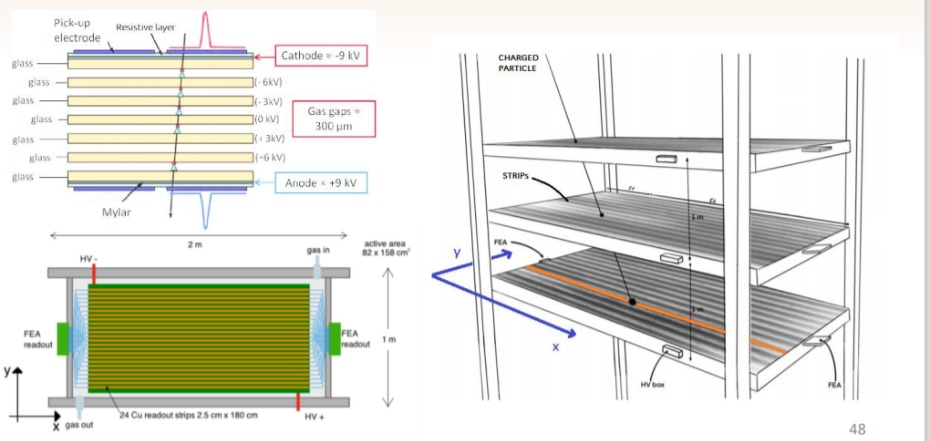
\includegraphics[width=0.9\linewidth]{progetto_EEE.jpeg} 
    \caption{MRPC del progetto EEE.}
    \label{fig:progetto_eee}
\end{figure}
Per tali rivelatori ogni layer è separato da un sottile filo da pesca, e la raccolta del segnale elettrico è effettuata tramite l'utilizzo di alcune striscioline di rame posizione sui diversi layer.


\chapter{Rivelatori basati su Scintillatori}
Lo \textit{scintillatore} è senza dubbio uno dei rivelatori di particelle più usati nella fisica nucleare e nella fisica delle particelle.\\
Esso utilizza il fatto che il passaggio di particelle o radiazioni produce in certi materiali (scintillatori) l'emissione di luce di scintillazione, se accoppiate a un dispositivo di amplificazione come un fotomoltiplicatore, queste scintillazioni possono essere convertite in impulsi elettrici che possono dare informazioni sulle caratteristiche delle particelle che hanno interagito con il materiale.
\section{Proprietà ideali di un scintillatore}
Un buon scintillatore dovrebbe possedere le seguenti proprietà:
\begin{itemize}
    \item Alta efficienza di scintillazione (conversione in luce dell’energia depositata con resa- $fotoni/MeV$- elevata);
    \item Una risposta lineare, cioè la luce prodotta dovrebbe essere proporzionale all'energia depositata, nel più ampio range possibile;
    \item Il mezzo scintillante dovrebbe essere trasparente alla propria luce di emissione in modo tale da non avere perdite di luce di scintillazione;
    \item Il tempo di decadimento piccolo in modo da generare in uscita un segnale veloce;
    \item Il materiale facilmente manipolabile, in modo da poterlo lavorare in diverse varietà di forme e dimensioni per adattarlo alle esigenze pratiche dei diversi rivelatori;
    \item L'indice di rifrazione vicino a quello del vetro (1.5), in modo da permettere il suo efficiente accoppiamento con con un fotomoltiplicatore;
\end{itemize}
Purtroppo nessun scintillatore possiede contemporaneamente tutte queste proprietà, quindi la scelta di un particolare tipo rispetto ad un altro dipende da vari fattori, e dalla particolare applicazione che richiede di ottimizzare una di queste caratteristiche.

\begin{itemize}
    \item LUMINESCENZA: emissione di fotoni  (luce visibile, UV, raggi X) dopo un assorbimento di energia. L'energia viene depositata nel materiale attraverso:
    \begin{itemize}
        \item luce $\rightarrow$ fotoluminescenza;
        \item calore $\rightarrow$ termoluminescenza;
        \item suono $\rightarrow$ sonoluminescenza;
        \item energia elettrica $\rightarrow$ elettroluminescenza;
        \item deformazioni meccaniche $\rightarrow$ triboluminescenza;
        \item reazioni chimiche $\rightarrow$ chemiluminescenza;
        \item organismi viventi $\rightarrow$ bioluminescenza;
    \end{itemize}
    \item SCINTILLAZIONE: emissione di fotoni a seguito di eccitazione di atomi e molecole indotta da radiazione (gamma o particelle):
    \begin{itemize}
        \item Fluorescenza:  emissione pronta di luce visibile da parte di atomi eccitati;
        \item Fosforescenza: emissione di luce con tempi caratteristici più grandi, e spettro di emissione con lunghezze d’onda maggiori;
        \item Fluorescenza ritardata: emissione con tempi caratteristici ancora maggiori ma lunghezze d’onda simili a quelle della fluorescenza.
    \end{itemize}
\end{itemize}

\section{Tipologie di scintillatori}
Esistono diverse categorie di scintillatori:
\begin{itemize}
    \item Scintillatori organici (a base di C,H,O):
    \begin{itemize}
        \item cristalli organici puri;
        \item liquidi organici;
        \item scintillatori plastici;
    \end{itemize}
    \item Scintillatori plastici
    \begin{itemize}
        \item cristalli inorganici;
        \item scintillatori a vetro (SiO2 + altro);
        \item scintillatori a gas;
    \end{itemize}
\end{itemize}

\section{Scintillatori organici}
In questi materiali, non cristallini, esiste una struttura di livelli atomici vibrazionali, ed elettronici (queste sono proprietà intrinseche alla molecole, non al suo stato fisico ovvero solido, liquido o gassoso)\footnote{Si consiglia di consultare i riassunti di struttura della materia per capire al meglio questo concetto.}.\\
A temperatura ambiente le molecole sono nello stato $S_{00}$ ma il processo di eccitazione/ionizzazione indotta dalla radiazione porta gli elettroni sui livelli $S_{1X}$, $S_{2X}$, $S_{3X}$,...
Gli stati elettronici/vibrazionali decadono velocemente (ordine dei ps) nello stato $S_{10}$ via transizioni non radiative. La radiazione pronta, ovvero la prompt fluorescence, viene emessa nella transizione tra lo stato $S_{10}$ e gli stati $S_{0X}$ con una legge di tipo esponenziale.
La radiazione ritardata (delayed phosphorescence) viene emessa dopo una transizione intra-bande che porta gli elettroni nello stato di tripletto (ordine dei $ms$).
\begin{center}
    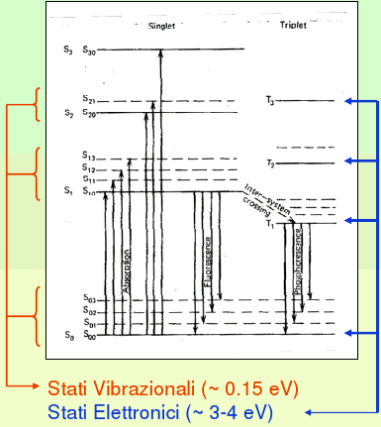
\includegraphics[width=8cm]{scint_org.png}
\end{center}
Questo meccanismo di decadimento impedisce alla luce di scintillazione di essere assorbita. Infatti, nel materiale, gli elettroni occupano solo lo stato $S_{10}$ in quanto non hanno abbastanza energia termica per saltare sul primo stato vibrazionale (solo la transizione diretta $S_{10}-S_{00}$ può essere assorbita).
Ogni materiale ha uno spettro caratteristico di emissione. A causa della struttura dei livelli, spettro di emissione e spettro di assorbimento sono spostati, per cui il materiale è circa trasparente alla luce emessa da se stesso.
\begin{center}
    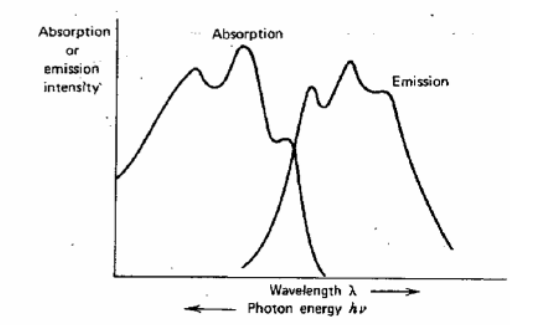
\includegraphics[width=8cm]{scint_org1.png}
\end{center}
Nella figura sottostante rappresenta un tipico spettro di emissione di uno scintillatore plastico.
\begin{center}
    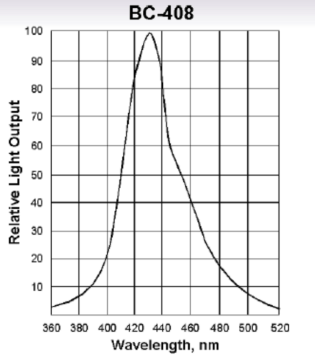
\includegraphics[width=8cm]{scint_org2.png}
\end{center}

\section{Scintillatori inorganici}
In questi materiali, cristallini, esiste una struttura a bande con un gap di energia tra le due bande è di
qualche decina di eV.
\begin{center}
    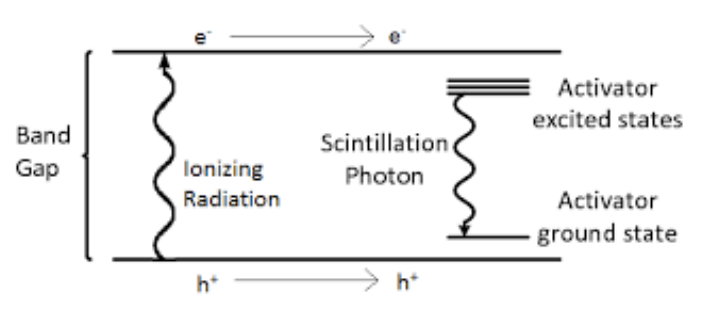
\includegraphics[width=8cm]{scin_ino.png}
\end{center}
Generalmente si aggiunge un drogante (attivatore) che crea stati energetici tra la banda di valenza e di conduzione che creano una via privilegiata di decadimento per la coppia elettrone-lacuna. Se l'attivatore è scelto opportunamente e se la sua concentrazione non è eccessiva le coppie elettrone-lacuna indotte dalla radiazione incidente si annullano attraverso l'emissione di luce visibile che non può essere riassorbita dallo scintillatore in quanto di energia inferiore al gap energetico.\\
Drogare un cristallo scintillatore organico significa rendere differente lo spettro della luce emessa da quello della luce assorbita. La conseguenza più diretta del drogaggio quindi è la riduzione dell'autoassorbimento.\\
Generalmente uno scintillatore inorganico ha una mediocre risposta temporale, ha una buona risoluzione energetica ed ha una emissione di luce che dipende dalla particella incidente.\\
Nella figura sottostante sono rappresentati spettri di emissione tipici di alcuni scintillatori inorganici.
\begin{center}
     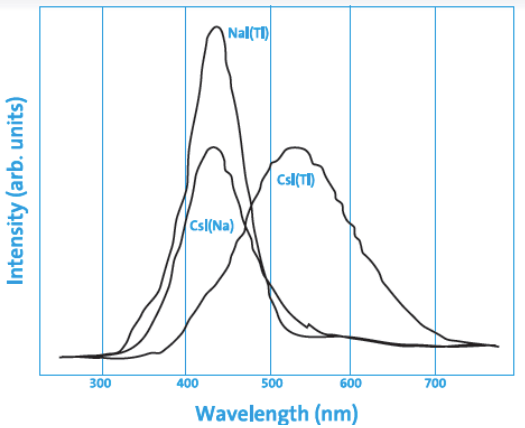
\includegraphics[width=8cm]{scin_ino1.png}
\end{center}
\section{esempi}
\begin{itemize}
    \item scintillatori inorganici:
    \begin{center}
        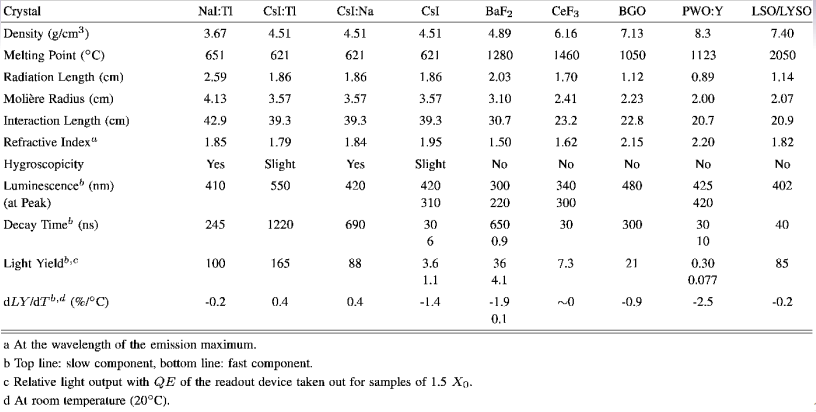
\includegraphics[width=12cm]{es_scint.png}
    \end{center}
    \item scintillatori plastici:
    \begin{center}
        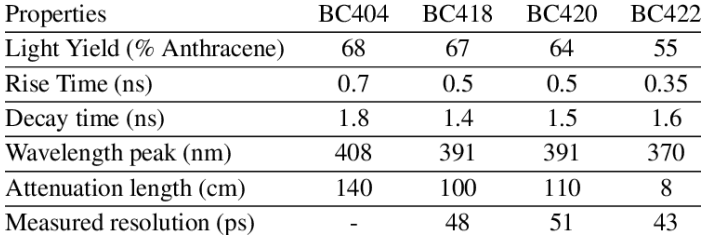
\includegraphics[width=8cm]{es_scint1.png}
    \end{center}    
\end{itemize}

\section{Risposta in luce}
L'intensità della luce di scintillazione è proporzionale all'energia persa dalla particella ionizzante nello scintillatore; perciò questi rivelatori forniscono informazioni sull'energia della particella.\\
La risposta in luce non è del tutto lineare con l'energia:
\begin{center}
    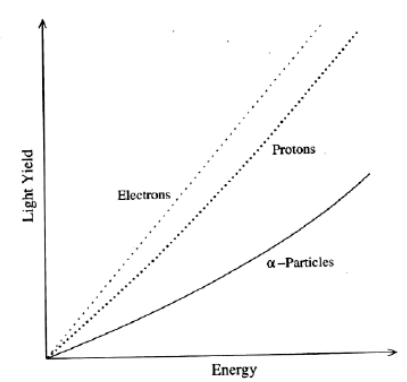
\includegraphics[width=6cm]{luce_scint.png}
\end{center}
Solo una frazione dell'energia depositata in uno scintillatore è convertita in luce; il resto da luogo a processi non radiativi. Questa frazione di energia depositata dipende dal tipo di particella e dall'energia depositata. Ad esempio, per uno scintillatore plastico la risposta in luce per protoni è circa 10 volte minore che per gli elettroni.\\
Il \textit{quenching}, ovvero il fenomeno che da luogo alla perdita di luce, indotto da particelle con alto $dE/dx$ è causato dalla presenza di molecole danneggiate dalla radiazione incidente e quindi non più in grado di scintillare. Posta $L$ la luce di scintillazione prodotta ed $S$ l'efficienza di scintillazione, nel caso ideale si ha:
$$\frac{dL}{dx}=S\frac{dE}{dx}$$
Mentre nel caso di quenching:
$$\frac{dL}{dx}=\frac{S\frac{dE}{dx}}{1+kB\frac{dE}{dx}}$$
nota come \textit{relazione di Birks}.
Il valore $N=B\frac{dE}{dx}$ è pari al numero di molecole danneggiate, $B$ è un parametro empirico di proporzionalità, $P=Nk=kB\frac{dE}{dx}$ è la percentuale di luce persa per effetto quenching.

\section{Risposta temporale}
Il profilo temporale di un impulso di luce in uno scintillatore può avere tempi di salita e tempi di discesa tra i nanosecondi e le centinaia di nanosecondi, a seconda dello scintillatore.
\begin{center}
    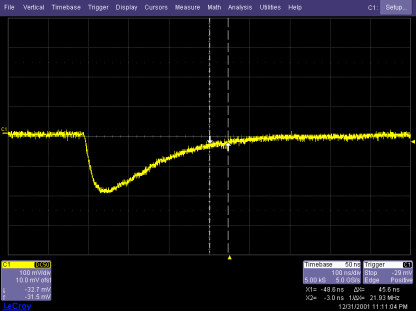
\includegraphics[width=7cm]{luce_scintillatore.png}
\end{center}

\section{Raccolta della luce}
La luce prodotta nello scintillatore lungo la traccia è emessa isotropicamente. Essa deve essere raccolta e misurata da un opportuno fotosensore.
Per fare questo lo scintillatore si riveste di un materiale riflettente. I fotoni di scintillazione possono essere riflessi dalle pareti fino a raggiungere il fotosensore. 
\begin{center}
    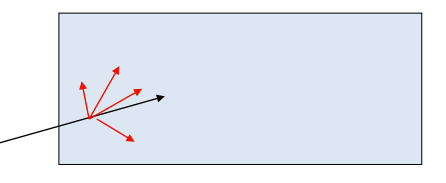
\includegraphics[width=6cm]{luce_scint1.png}
    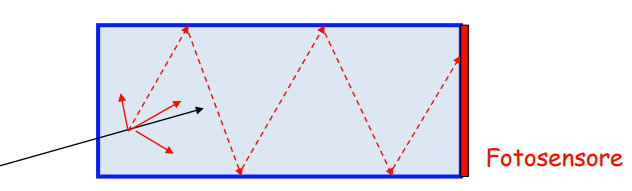
\includegraphics[width=8cm]{luce_scint2.png}
\end{center}
Avvengono due processi di assorbimento per i fotoni di scintillazione:
\begin{itemize}
    \item Assorbimento nel materiale (Self-absorption), che segue una legge esponenziale del tipo:
    $$I=I_0e^{-\frac{x}{L}}$$
    dove L è il parametro di attenuazione;
    \item Assorbimento alle pareti, sono parzialmente riflettenti.
\end{itemize}
Alle pareti si può avere una riflessione \textit{diffusa} (ad esempio con uno strato bianco opaco di Teflon, vernice,...) o \textit{speculare} (ad esempio con uno strato di alluminio sottile). 
La superficie può essere inoltre \textit{liscia} o “\textit{rugosa}”.
\begin{center}
    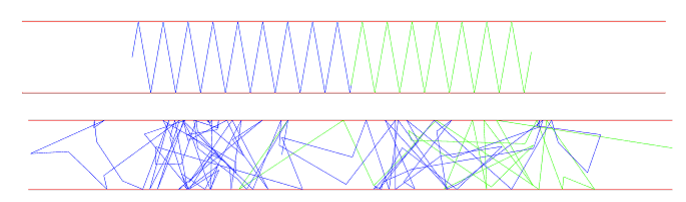
\includegraphics[width=8cm]{luce_scint3.png}
\end{center}
Il fenomeno della raccolta della luce in scintillatori è oggetto di simulazioni professionali (esempio: codice GEANT4), che tengono conto di diversi fattori. Ad esempio la riflettività da parte della superficie alluminizzata può essere considerata come dipendente dalla lunghezza d’onda, anziché costante.

\section{Guide di luce}
Quando le dimensioni dello scintillatore non si adattano bene a quelle del fotosensore, si impiega una guida di luce (ad esempio in plexiglas).
Devono essere sagomate in modo da convogliare quanta più luce un’estremità all'altra.\\
La frazione di luce max raccolta è pari al rapporto delle adiabatiche:
$$F=\frac{A_{fotosensore}}{A_{scintillatore}}$$
\begin{center}
    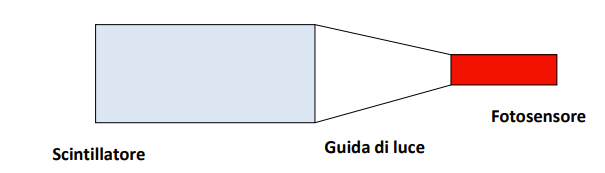
\includegraphics[width=8cm]{luce_scint4.png}
\end{center}
Una tecnica diversa, per raccogliere la luce di scintillazione in rivelatori lunghi, è quella di usare \textit{fibre WLS} (WaveLenght Shifter), immerse nello scintillatore.\\
Esse assorbono la luce di scintillazione, la riemettono a adatte al tipo di fotosensore impiegato) e la trasportano come delle fibre ottiche, con bassa attenuazione.

\section{Rivelatori basati su scintillatori}
Gli scintillatori vengono impiegati in diversi campi della fisica: fisica nucleare, astroparticellare, fisica applica, in particolare applicata nel campo medico. Un esempio di applicazione è la \textit{tomografia a emissione di positroni} o \textit{PET} è una tecnica di medicina nucleare e di diagnostica medica utilizzata per la produzione di bioimmagini.
\begin{center}
    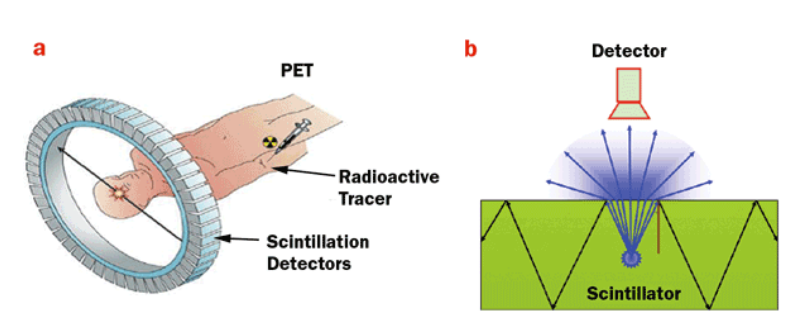
\includegraphics[width=8cm]{PET.png}
\end{center}
La procedura inizia con l'assunzione del soggetto da esaminare di un radiofarmaco formato da un isotopo tracciante con breve tempo di dimezzamento legato chimicamente ad una molecola attiva a livello metabolico. L'isotopo, dopo un breve lasso temporale, decade emettendo un positrone. Dopo un percorso che può raggiungere al massimo pochi millimetri, il positrone si annichila con un elettrone, producendo una coppia di fotoni gamma emessi in direzioni opposte tra loro.\\
Questi fotoni sono rilevati quando raggiungono uno scintillatore, nel dispositivo di scansione, dove creano un lampo luminoso, rilevato attraverso tubi fotomoltiplicatori. Punto cruciale della tecnica è la rivelazione simultanea di coppie di fotoni. Dalla misurazione della posizione in cui i fotoni colpiscono il rilevatore, si può ricostruire la posizione del corpo da cui sono stati emessi permettendo la determinazione dell'attività chimica all'interno del corpo da investigare.



\chapter{Fotosensori}
La luce di scintillazione prodotta in un mezzo dal passaggio di una radiazione può essere raccolta da opportuni fotosensori, per produrre un segnale elettrico e dare informazioni sulla radiazione originaria.\\
Esempi di fotosensori attualmente usati:
\begin{itemize}
    \item Fotomoltiplicatori;
    \item Avalanche photodiodes (APD);
    \item Silicon photomultipliers (SiPM).
\end{itemize}

\section{Fotomoltiplicatori}
Tipicamente un \textit{fotomoltiplicatore} è costituito da un catodo in materiale fotosensibile seguito da un sistema di raccolta di elettroni, cioè una stringa di \textit{dinodi}, e infine un anodo da cui si può prelevare il segnale finale. Tutte le componenti sono solitamente alloggiate in un tubo di vetro sottovuoto.
\begin{center}
    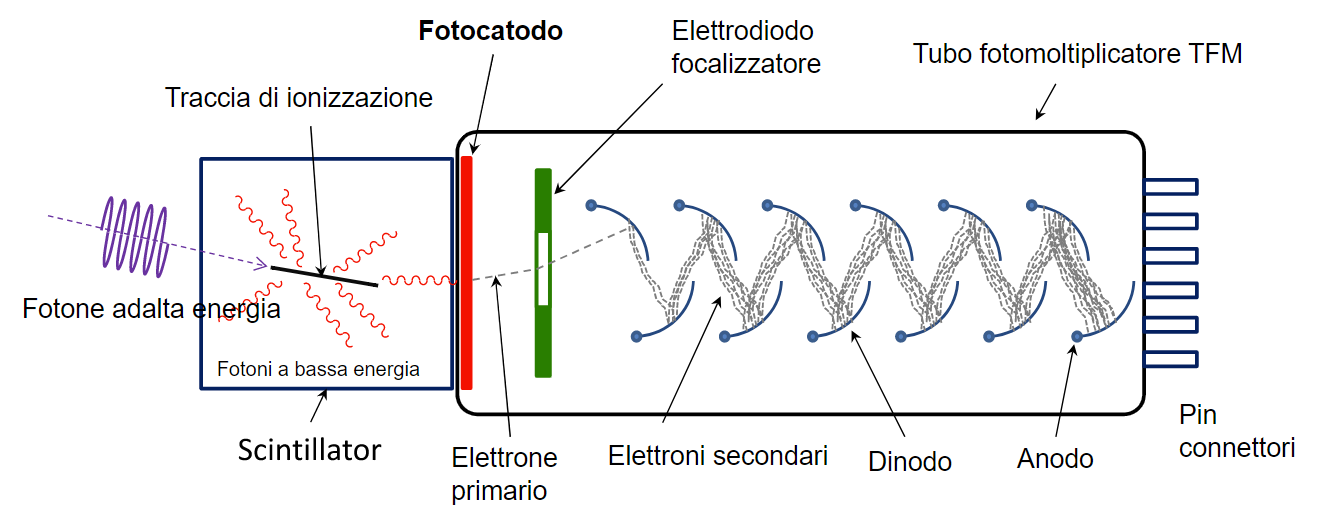
\includegraphics[width=8cm]{fotomoltiplicatore.png}
\end{center}
Durante il funzionamento viene applicata un'alta tensione al catodo, ai dinodi e all'anodo in modo tale da creare una potenziale "scala" lungo la lunghezza della struttura catodo - dinodo - anodo.\\ 
Quando un fotone incidente (ad esempio da uno scintillatore) colpisce il fotocatodo, viene emesso un elettrone tramite l'effetto fotoelettrico. A causa della tensione applicata, l'elettrone viene quindi diretto e accelerato verso il primo dinodo, dove colpendo trasferisce parte della sua energia agli elettroni nel dinodo. Ciò provoca l'emissione di elettroni secondari, che a loro volta vengono accelerati verso il dinodo successivo dove vengono rilasciati più elettroni e ulteriormente accelerati. Viene così creata una cascata di elettroni lungo la stringa del dinodo. Arrivata all'anodo questa cascata viene raccolta per fornire una corrente che può essere amplificata e analizzata.\\
I fotomoltiplicatori possono funzionare in modalità\textit{ continua}, cioè sotto un'illuminazione costante, o in modalità \textit{pulsata} come nel caso del conteggio a scintillazione. In entrambe le modalità, se si assume che i sistemi catodo e dinodo siano lineari, la corrente all'uscita del fotomoltiplicatore sarà direttamente proporzionale al numero di fotoni incidenti.\\
Un rivelatore di radiazione prodotto accoppiando uno scintillatore ad un fotomoltiplicatore (lo scintillatore produce fotoni in proporzione all'energia depositata nello scintillatore) sarebbe quindi in grado di fornire non solo informazioni sulla presenza della particella ma anche sull'energia che essa ha lasciato nello scintillatore.

\section{Fotocatodo}
Il \textit{fotocatodo} converte la luce incidente in una corrente di elettroni per effetto fotoelettrico.
Energia fotoni luce scintillazione: circa $3 eV$.\\
Per facilitare il passaggio di questa luce, il fotocatodo viene rivestito da un materiale semiconduttore con lavoro di estrazione di circa $2-1.5eV$.\\
Vi è la possibilità che alcuni di questi elettroni vengono emessi spontaneamente per effetto termico. L'energia media degli elettroni a T ambiente è uguale $0.025 eV$, la distribuzione in energia degli elettroni fa sì che una certa frazione possa avere energia sufficiente a sfuggire. L'effetto di questa emissione è la \textit{dark current}, cioè corrente di elettroni anche in assenza di 
radiazione incidente.\\
Uno dei parametri che definiscono un fotomoltiplicatore è la \textit{Quantum Efficiency}:
$$QE=\frac{N. fotoelettroni emessi}{N. fotoni incidenti}$$
I valori tipici sono circa del $20-30\%$. La Quantum Efficiency è fortemente dipendente dalla lunghezza d’onda.

\section{Dinodi}
Gli elettroni emessi per effetto fotoelettrico devono essere convogliati verso il sistema di dinodi, per fare ciò viene utilizzato un campo elettrico. In linea di principio possono essere utilizzati anche campi magnetici o una combinazione di campi elettrici e magnetici, ma il loro uso è estremamente raro. Indipendentemente dal design, devono essere soddisfatti due requisiti importanti:
\begin{itemize}
    \item La raccolta deve essere efficiente e indipendente dal punto di emissione dalla superficie del fotocatodo;
    \item Il tempo di percorrenza dal catodo al primo dinodo deve essere indipendente dal punto di emissione ($\rightarrow$ timing).
\end{itemize}
\begin{center}
    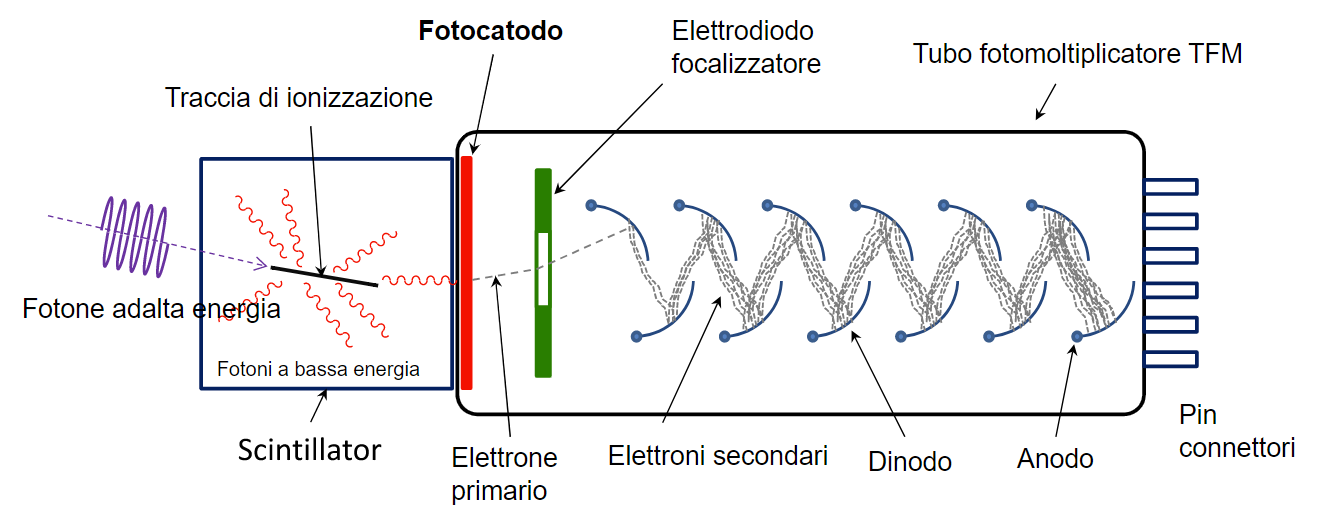
\includegraphics[width=8cm]{fotomoltiplicatore.png}
\end{center}
Il sistema di dinodi amplifica il numero di elettroni tramite emissioni secondarie. 
Il primo dinodo ha un potenziale più positivo rispetto al fotocatodo, perciò l’elettrone primario accelera verso di esso. Qui avviene l’emissione secondaria: il dinodo emette elettroni. Questi elettroni, detti secondari, sono accelerati verso il dinodo successivo, che è più positivo del primo. Il meccanismo si ripete quindi per tutti i dinodi: l’emissione secondaria moltiplica il numero di elettroni e il campo elettrico li accelera. La cascata di elettroni prodotta è raccolta dall’anodo, l’elettrodo con il potenziale più positivo di tutti, posto alla fine del percorso, generando un impulso elettrico misurabile. La catena di dinodi permette di avere una moltiplicazione esponenziale del numero di elettroni: a partire da un solo elettrone primario prodotto dalla luce incidente si possono ottenere centinaia di milioni di elettroni secondari.\\
Esistono diversi tipi di dinodi a seconda 
\begin{itemize}
    \item del materiale: quelli di uso comune oggi sono $Ag - Mg$,$ Cu - Be$ e $Cs - Sb$;
    \item della configurazione: le più comuni sono:
    \begin{itemize}
        \item[a)] a veneziana;
        \item[b)] a box e a griglia;
        \item[c)] focalizzati linearmente;
        \item[d)] focalizzati circolarmente
    \end{itemize}
\end{itemize}
\begin{center}
    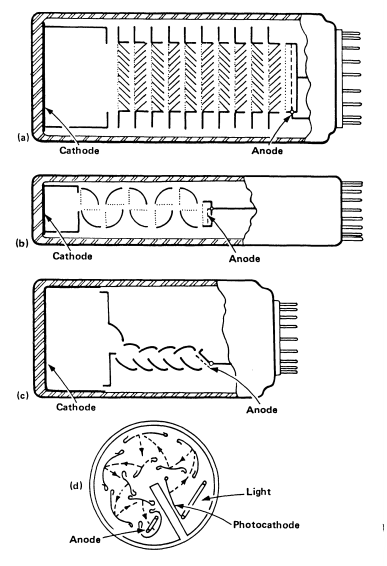
\includegraphics[width=6cm]{dinodi.png}
\end{center}
La tensione di alimentazione è distribuita tra i vari dinodi mediante partitori di tensione, con condensatori o diodi zener in parallelo.\\
In genere tra fotocatodo e primo dinodo è applicata una tensione maggiore, allo scopo di focalizzare meglio gli elettroni emessi dal fotocatodo.\\
La polarità può essere stabilita in 2 modi equivalenti, con il fotocatodo a $-HV$ e l\textquotesingle anodo a zero, oppure fotocatodo a zero e anodo a $+HV$.\\
Il guadagno complessivo $G$, cioè il numero totale di elettroni prodotti per fotone incidente in un fotomoltiplicatore a n dinodi è:
$$G=\alpha\delta^n$$
dove $\delta$ è il \textit{fattore di emissione di elettroni secondari} di ogni dinodo, cioè il rapporto tra elettroni secondari e primari; esso rappresenta il guadagno di un singolo dinodo.\\
Tuttavia il valore di $\delta$ non è costante da evento a evento. Le sue fluttuazioni possono essere descritte in prima approssimazione da un distribuzione di Poisson, con valor medio $\delta$ e deviazione standar $\sqrt{\delta}$, questo vale nel caso di una sola amplificazione. Dopo $n$ stadi di amplificazione ($n$ dinodi) il valor del numero di elettroni secondari è $\delta^n$.\\
Quando l’evento è iniziato da un grande numero (decine/centinaia) di fotoelettroni, il segnale è molto più grande del rumore, prodotto in genere da singoli fotoelettroni, altrimenti può confondersi con il rumore.\\
Il fattore di moltiplicazione è proporzionale alla tensione di alimentazione:
$$\delta \propto V_d^{\alpha}$$
con $V_d$ è la tensione applicata ad un dinodo e $\alpha$ è un fattore correttivo, tipicamente compreso tra $0.7$ e $0.8$.\\
Il guadagno totale G di un fotomoltiplicatore è dato dal prodotto dei guadagni dei singoli dinodi.  Nel caso in cui il fattore di moltiplicazione sia lo stesso per tutti i dinodi, perchè supponiamo la tensione applicata sia equamente divisa tra i dinodi, il guadagno complessivo del fotomoltiplicatore è quindi la legge di potenza:
$$G=\delta^n=(kV_d)^n \propto V^n$$
con $k$ costante di proporzionalità e V tensione di alimentazione del fotomoltiplicatore, che vale $V=(N+1)V_{dinodo}$; questa equazione mostra che vi è una relazione di potenza tra il guadagno del PMT e la tensione alla quale è alimentato.\\
Un importante grandezza che si può considerare è il coefficiente di guadagno che esprime la variazione in $\%$ del guadagno rispetto alla tensione applicata:
$$\frac{1}{G}\frac{dG}{dV}$$
espressa in $\%/V$.

\newpage
\section{Risposta temporale}
Due fattori principali influenzano la risoluzione temporale dei fotomoltiplicatori:
\begin{enumerate}
    \item Variazioni nel tempo di transito (di circa qualche $ns$) degli elettroni attraverso il fotomoltiplicatore;
    \item Fluttuazioni dovute al rumore statistico.
\end{enumerate}
Le variazioni del tempo di transito possono verificarsi a causa delle differenze nella lunghezza del tratto percorso dagli elettroni e nell'energia con cui vengono emessi dal fotocatodo.
La differenza di lunghezza percorsa è ulteriormente accresciuta dall'asimmetria del dinodo. 
Chiaramente gli elettroni emessi dal bordo inferiore, di un generico dinodo, hanno una distanza maggiore da percorrere rispetto a quelli dal bordo superiore dell'elettrodo. Questo effetto è noto come \textit{differenza di tempo di transito} ed è associato a
la geometria del sistema.
Un'ovvia soluzione è l'utilizzo di un catodo sferico, in modo da pareggiare meglio le distanze.\\
Un modo più efficace, tuttavia, è quello di graduare il campo elettrico in modo tale che gli elettroni sul bordo vengano accelerati più di quelli sull'asse.
Oltre agli effetti geometrici, si verificheranno anche variazioni che dipendono dall'energia e dalla direzione degli elettroni emessi.\\
Chiaramente gli elettroni emessi con un'energia elevata raggiungeranno il dinodo più velocemente di quelli a energie inferiori. Analogamente, gli elettroni emessi in una direzione più vicina alla normale del catodo arriveranno prima di quelli emessi in una direzione parallela alla superficie.\\
Questo effetto è chiamato \textit{diffusione del tempo di transito} ed è indipendente dal punto in cui l'elettrone lascia il catodo.

\section{Schermo magnetico}
Poichè gli elettroni all'interno del fotomoltiplicatore hanno energie molto basse e (pochi eV- centinaia di eV), possono essere deviati facilmente da un campo magnetico, come abbiamo già visto.\\
In presenza di campi magnetici un PMT deve essere schermato con schermi in \textit{mu-metal} (lega metallica ad alta permeabilità magnetica). Anche il campo magnetico terrestre può influenzare il comportamento di un PMT, infatti il guadagno può variare a seconda dell’orientazione rispetto al campo magnetico.\\
In rivelatori di particelle, posti all’interno di grandi magneti, l’uso di fotomoltiplicatori 
è precluso, e bisogna utilizzare altri tipi di fotosensori.

\section{Noise}
Anche quando un fotomoltiplicatore non è illuminato, scorre ancora una piccola corrente. Questa corrente è chiamata \textit{dark current} e deriva da diverse fonti:
\begin{enumerate}
    \item emissione termoionica dal catodo e dai dinodi:\\
    il contributo di questo rumore non può essere trascurabile se il valore medio del numero di fotoelettroni dal segnale «vero» è piccolo. Il rumore può essere diminuito abbassando la temperatura
    \item correnti di dispersione;
    \item contaminazione radioattiva;
    \item fenomeni di ionizzazione;
    \item fenomeni luminosi;
\end{enumerate}
con il rumore termico come componente principale.\\
Un altro problema che potrebbe causare una scarsa efficienza del PMT è \textit{afterpulses}, cioè : impulsi che seguono l’impulso principali, sono importanti specialmente in misure di timing.
\begin{itemize}
    \item \textit{Reazioni luminose}: i dinodi colpiti dagli elettroni possono emettere fotoni che, se arrivano al fotocatodo, danno origine ad afterpulses (efficienza bassa). Ritardi tipici di $20-100 ns$;
    \item \textit{Ionizzazione gas residui}: gli elettroni possono ionizzare il gas residuo e gli ioni positivi prodotti driftano verso il fotocatodo, liberando elettroni. Ritardi tipici $100 di ns - \mu s$;
    \item \textit{Backscatter degli elettroni}: durante il processo di amplificazione, alcuni elettroni possono essere rimandati indietro dall’urto, ritornando al primo dinodo e generando un altro segnale ritardato rispetto al primo.
\end{itemize}

\section{Forma e applicazioni di un PMT}
In genere hanno una forma cilindrica, con un diametro che può andare da pochi $cm$ ad alcune decine di $cm$.\\
Data l’estrema sensibilità ai fotoni, i fotomoltiplicatori sono adoperati in tutte le applicazioni in cui è necessario rivelare luce di bassa intensità:
\begin{itemize}
    \item luce di scintillazione da scintillatori;
    \item luce Cerenkov prodotta nell’atmosfera;
    \item luce raccolta da telescopi ottici, in astronomia;
    \item in medicina (diagnostica per immagini) e biologia (bioluminescenza),...
\end{itemize}
I PMT vengono utilizzati anche vari esperimenti, tra cui:
\begin{itemize}
    \item L'esperimento \textit{Super-Kamiokande}, in cui ne vengono impiegati circa $10000$ per rivelare i neutrini;
    \item L’esperimento \textit{WA98} al CERN impiega oltre 10000 fotomoltiplicatori per rivelare la luce di scintillazione prodotta nei cristalli del calorimetro elettromagnetico;
    \item L’esperimento \textit{Auger} impiega oltre 10000 fotomoltiplicatori per rivelare la luce di fluorescenza prodotta nell’atmosfera dai cosmici;
    \item L’esperimento \textit{AMS (AntiMatterSearch)} a bordo della Stazione Spaziale Internazionale si impiegano fotomoltiplicatori.
\end{itemize}

\section{Altri fotosensori}
In molte applicazioni, i tradizionali fotomoltiplicatori presentano dei problemi:
\begin{itemize}
    \item Dimensioni talvolta troppo grandi rispetto all’area sensibile;
    \item Influenzati dai campi magnetici;
    \item Risposta spettrale non sempre adatta alla luce da rivelare;
    \item Efficienza quantica non elevata;
    \item Stabilità del guadagno non sempre ottimale;
    \item Tensioni di alimentazione elevata (kV).
\end{itemize}
In tempi più recenti sono stati sviluppati fotosensori più compatti a stato solido, in 
particolare:
\begin{itemize}
    \item Avalanche photodiodes (APD);
    \item Silicon photomultipliers (SiPM)
\end{itemize}

 \section{Avalanche photodiodes (APD)}
Un \textit{fotodiodo a valanga}, brevemente detto \textit{APD} (dall'inglese Avalanche PhotoDiode), è un particolare tipo di fotodiodo che funziona come sensore ottico in grado di riconoscere una determinata lunghezza d'onda e di trasformare questo evento in un segnale elettrico di corrente amplificandolo al suo interno. Dal punto di vista circuitale, il fotodiodo a valanga è quasi identico al fotodiodo.
\begin{center}
    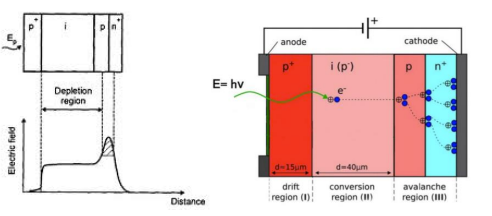
\includegraphics[width=10cm]{apd.png}
\end{center}
Un fotodiodo a valanga è sostanzialmente un fotodiodo particolare caratterizzato solitamente da 4 strati di semiconduttore drogati asimmetricamente. Abbiamo quindi, in sequenza, queste zone:
\begin{enumerate}
    \item a zona $p+$, cioè una zona molto drogata con ${N_{a}}$ accettori;
    \item la zona intrinseca di semiconduttore che serve a tenere quasi costante il campo elettrico, serve ad aumentare l'efficienza quantica e a diminuire la capacità di giunzione;
    \item la zona $p$, una zona drogata con ${N_{a}}$ accettori, ma in quantità inferiore alla prima;
    \item la zona $n+$, zona caratterizzata dalla presenza di molti atomi ${N_{d}}$ donatori.
\end{enumerate}
La terza zona, o zona $p$, rappresenta la parte fondamentale del fotodiodo a valanga, perché permette l'effetto moltiplicativo o di guadagno delle cariche. In pratica, le cariche primarie prodotte nella zona intrinseca per effetto fotoconduttivo, creano un effetto valanga che genera un numero elevato di cariche secondarie. Queste cariche secondarie quindi saranno quelle che generano la corrente prodotta dal fotodiodo.\\
Gli svantaggi e i vantaggio del fotodiodo a valanga sono:
\begin{itemize}
    \item A causa di uno strato anti-riflesso in superficie, la maggior parte dei fotoni è convertita in segnale, con efficienze dell’ordine dell’$80\%$;
    \item La tensione di alimentazione è di alcune centinaia di volt (tensioni di lavoro non particolarmente elevate);
    \item Guadagni non elevatissimi, dell’ordine di $50-100$;
    \item Alta sensibilità alla temperatura, necessitano di correzioni (qualche $\%$ per ogni grado di variazione), è uno svantaggio perchè la risposta del rivelatore può variare con la temperatura;
    \item Particolarmente adatti a convertire la luce proveniente da fibre WLS o da piccoli scintillatori;
    \item Proprietà temporali buone
    \item  Dimensioni da $1x1$ a $5x5 mm^2$ e oltre.
\end{itemize}
Gli APD sono utilizzati nei \textit{calorimetri elettromagnetici}, ad esempio quelli dell'esperimento \textit{ALICE@LHC} utilizzano circa 20000 APD per leggere la luce di scintillazione prodotta nei moduli di rivelazione, attraverso fibre WLS.\\

\section{Silicon photomultipliers (SiPM)}
A differenza dei fotomoltiplicatori tradizionali, costruiti con tubi a vuoto, i \textit{SiPM} sono prodotti direttamente da un wafer di silicio su cui vengono impiantate matrici costituite da array di microcelle su un comune substrato in silicio. Ciascuna microcella è un fotodiodo a valanga a singolo fotone. L'idea di base è la rilevazione di eventi a singolo fotone in APD connessi in sequenza. Le dimensioni di una singola cella vanno dalle decine alle centinaia di micron (densità dell’ordine di $1000/mm^2$). Ogni cella lavora in modo (quasi) indipendente. Un fotone dà segnale in una cella, ma non (in prima approssimazione) nelle altre.
\begin{center}
    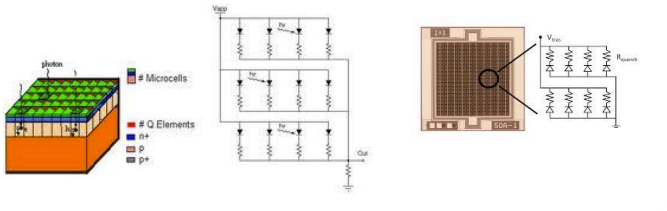
\includegraphics[width=10cm]{simp.png}
\end{center}
Gli svantaggi e i vantaggi dei SiPM sono:
\begin{itemize}
    \item Lavorano a tensione molto bassa (30-70 V);
    \item Efficienza quantica: $20-40\%$;
    \item Guadagni elevati, fino a $10^6$;
    \item Risoluzione temporale molto buona ($<< 1ns$);
    \item Indipendenti dal campo magnetico;
    \item Tuttavia:
    \begin{itemize}
        \item  dimensioni ancora piccole, circa $10-50 mm^2$;
        \item dark count rate molto elevati ($100 kHz-1 MHz /mm^2$).
    \end{itemize}
\end{itemize}
Prendendo la somma di tutte le celle colpite, si può valutare quante celle sono state interessate, e quindi quanti fotoni sono stati rivelati.\\
Tutte le celle sono lette in parallelo. Anche se ogni cella dà un segnale ON/OFF la matrice genera un segnale analogico, proporzionale entro certi limiti al numero di fotoni che la 
colpiscono.\\
L’\textit{efficienza di rivelazione} dei fotoni (PDE, Photon Detection Efficiency) indica la frazione di fotoni incidenti rivelati dal SiPM e quindi esprime la capacità del dispositivo di rivelare fotoni. Essa è il risultato di tre fattori:
\begin{itemize}
    \item  Fill factor geometrico;
    \item  La quantum efficiency (QE), dipendente dalla lunghezza d’onda;
    \item La probabilità di trigger della valanga (dipende dalla tensione).
\end{itemize}
Il \textit{fill factor} è il rapporto tra l'area attiva e l'area totale, dipende dal design e dalle dimensione delle celle, infatti celle più piccole danno fill factor minori.\\
Ad esempio celle piccole da $20$ micron danno Fill factor dell’ordine del $30\%$, mentre celle da $100 $micron possono arrivare a fill factor
dell’$80\%$.\\
L’\textit{efficienza quantica QE} è definita come il numero medio di coppie elettroni-lacuna creato dal fascio incidente, essa può  essere anche molto elevata, dell'ordine dell'$80-90\%$.\\
La \textit{probabilità di triggerare} una valanga dipende dalla posizione in cui è stata creata la carica, dal tipo di carica (elettrone/lacuna) e dalla tensione di alimentazione.\\
In molte applicazioni, i SiPM sono usati per la lettura della luce trasportata da fibre WLS poste all'interno di scintillatori.
\section{Confronto tra fotosensori}
\begin{center}
    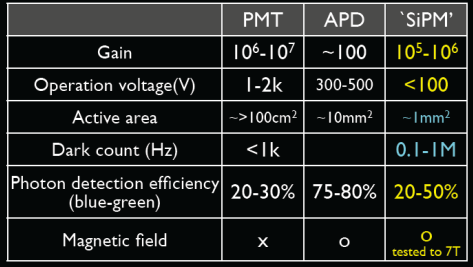
\includegraphics[width=14cm]{fotosensori.png}
\end{center}

\section{L'occhio umano}
La luce entra nell'occhio attraverso la cornea. ... I coni e i bastoncelli della retina assorbono la luce e inviano messaggi al cervello tramite il nervo ottico. Il cervello trasforma questi impulsi in un'immagine.
\begin{center}
    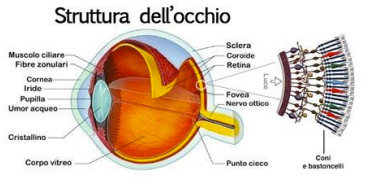
\includegraphics[width=9cm]{occhio.png}
\end{center}
\begin{itemize}
    \item \textbf{Coni}: localizzati nella parte centrale, destinati alla percezione dei colori, sono circa 6-7 milioni;
    \item \textbf{Bastoncelli}: localizzati nella zona periferica, particolarmente sensibili anche a pochi fotoni, sono circa 120 milioni.
\end{itemize}
\begin{center}
    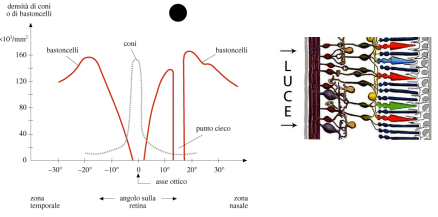
\includegraphics[width=14cm]{occhio2.png}
\end{center}
Facendo alcune stime la risoluzione dell'occhio umano, approssimandolo a una fotocamera, è di $570$ Mpixel.\\
Nella figura seguente si osserva il grafico della risposta spettrale (curva di sensibilità) dell'occhio umano.
\begin{center}
    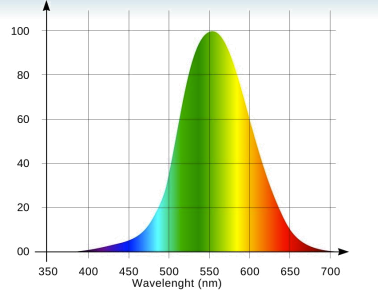
\includegraphics[width=10cm]{occhio3.png}
\end{center}

\chapter{Rivelatori a semiconduttore}
I rivelatori a semiconduttore, come suggerisce il nome, sono basati su materiali semiconduttori cristallini, in particolare silicio e germanio.\\
Questi rivelatori sono anche indicati come rivelatori a stato solido, sebbene il lavoro sui rivelatori di cristalli sia stato eseguito già negli anni $'30$, i primi prototipi passarono rapidamente allo stato di funzionamento e alla disponibilità commerciale negli anni $'60$.\\
Il principio di funzionamento di base dei rivelatori a semiconduttore è analogo ai rivelatori a gas. Invece di un gas, tuttavia, il mezzo è ora un materiale semiconduttore solido. Il passaggio della radiazione ionizzante crea coppie elettrone-lacuna (anziché coppie di elettroni) che vengono poi raccolte da un campo elettrico. Il vantaggio del semiconduttore, tuttavia, è che l'energia media richiesta per creare una coppia elettrone-lacuna è circa 10 volte inferiore a quella richiesta per la ionizzazione del gas. Pertanto la quantità di ionizzazione prodotta per una data energia è di un ordine di grandezza maggiore, con un conseguente aumento della risoluzione energetica. Inoltre, a causa della loro maggiore densità, hanno uno stopping-power maggiore rispetto ai rivelatori di gas. Sono di dimensioni compatte e possono avere tempi di risposta molto rapidi. Ad eccezione del silicio, tuttavia, i semiconduttori generalmente richiedono il raffreddamento a basse temperature prima di poter essere utilizzati. Ciò, ovviamente, implica un sistema aggiuntivo che aumenta il sovraccarico del rivelatore. Uno dei problemi dell'attuale ricerca sui rivelatori a semiconduttore, infatti, è trovare e sviluppare nuovi materiali che possano funzionare a temperatura ambiente. Essendo materiali cristallini, hanno anche una maggiore sensibilità ai danni da radiazioni che ne limita l'uso a lungo termine.\\
Come si nota nella figura sottostante gli elettroni sono capaci di occupare solo livelli discreti di energia. La banda più bassa viene chiamata \textit{banda di valenza}, quella più alta \textit{banda di conduzione}; quest'ultima contiene gli elettroni che sono capaci di interagire con altri atomi, essa è responsabile delle proprietà chimiche dell'atomo e dunque stabilisce se esso è un conduttore, un isolante o un semiconduttore. Fra le due bande esiste una zona, che in condizioni normali risulta inaccessibile agli elettroni; questa prende il nome di \textit{gap proibito di energia}.
\begin{center}
    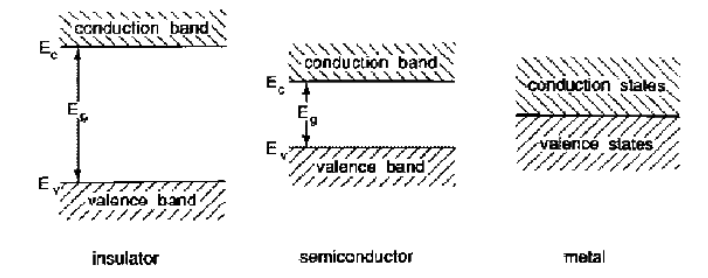
\includegraphics[width=10cm]{semicond.png}
\end{center}
Quando il gap proibito è tale che le fluttuazioni termiche che avvengono a temperatura ambiente riescono a far transitare un elettrone dalla banda di valenza alla banda di conduzione si parla di un conduttore, in caso contrario di un isolante. Un semiconduttore ha invece un gap proibito intermedio fra i due (circa $1eV$); esso viene definito come una sostanza la cui banda di valenza allo zero assoluto è completamente piena; a temperatura ambiente esistono alcuni elettroni termici eccitati che superando il gap conducono elettricità.\\
Comprendere ciò che è stato appena detto risulta importante per capire cosa avviene quando un cristallo semiconduttore viene investito da una radiazione nucleare. Quando una particella entra nel cristallo essa può ionizzare il cristallo eccitando un elettrone dalla banda di valenza alla banda di conduzione, creando una coppia elettrone-lacuna.\\
A temperature normali, in presenza di un campo elettrico:
\begin{itemize}
    \item Isolante: non c’è corrente;
    \item Conduttore: si genera una corrente;
    \item Semiconduttore: si osserva una piccola corrente (dovuta ad elettroni “termici”).
\end{itemize}
I portatori di carica in un semiconduttore sono gli \textit{elettroni} e le \textit{lacune}.\\
In un semiconduttore coesistono due fenomeni:
\begin{itemize}
    \item Creazione coppie elettrone-lacuna (per effetti termici);
    \item Ricombinazione.
\end{itemize}

\section{Semiconduttori puri}
In un semiconduttore puro (intrinseco) il numero di elettroni in banda di conduzione è eguale esattamente al numero di lacune in banda di valenza. Sia gli elettroni che le lacune contribuiscono alla conducibilità elettrica.\\
La struttura cristallina di semiconduttori quali il silicio e il germanio consiste in una ripetizione regolare in tre dimensioni di una cella unitaria a forma di tetraedro con un atomo in ogni vertice. Il silicio, ad esempio, è tetravalente ed ognuno dei quattro elettroni di valenza è messo in comune con uno dei quattro atomi vicini. Una struttura così ordinata priva di
imperfezioni crea quelli che vengono chiamati \textit{semiconduttori intrinseci}.
\begin{center}
    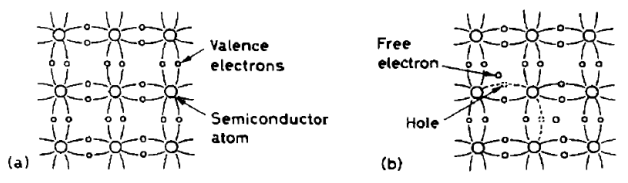
\includegraphics[width=10cm]{semicond1.png}
\end{center}
In un semiconduttore le coppie elettrone-lacuna sono costantemente formate dall'energia termica, ma nello stesso tempo alcune di esse si ricombinano. In condizioni di stabilità si crea un equilibrio nella concentrazione delle coppie. In un semiconduttore intrinseco la concentrazione di elettroni e lacune è uguale; indicando con $n_i$ tale concentrazione e con $T$ la temperatura si può dimostrare che vale la formula, chiamata dell'\textit{azione di massa}:
$$n_i=\sqrt{N_CN_V}\exp\left({\frac{-E_g}{2kT}}\right)=AT^{2/3}\exp\left({\frac{-E_g}{2kT}}\right)$$
dove $N_C$ è il numero di stati nella banda di conduzione, $N_V$ il numero di stati nella banda di valenza,
$E_g$ il gap energetico a $0^\circ K$ e $k$ la costante di Boltzmann. $N_C$ e $N_V$ possono essere calcolati tramite la statistica di Fermi-Dirac che mostra la loro dipendenza da $T^{2/3}$.\\
Tipicamente i valori di $n_i$ sono di $2.5 \times 10^{13}\,\mathrm{cm}^{-3}$ per il germanio e di $1.5 \times 10^{10}\,\mathrm{cm}^{-3}$ per il silicio ad una temperatura di $300^\circ K$. Sapendo che questi materiali hanno una densità media di $10^{22}$ atomi al $cm^3$, si comprende che solo 1 ogni $10^{9}$ atomi di germanio e 1 ogni $10^{12}$ atomi di silicio è ionizzato.\\
Quindi malgrado il grande esponente la concentrazione è molto bassa.\\
Quando viene applicato un campo elettrico, la velocità di deriva per elettroni e lacune può essere scritta come:
$$v_e=\mu_eE$$
$$v_l=\mu_l E$$
dove $E$ rappresenta il campo elettrico, $\mu_e$
la \textit{mobilità degli elettroni} e $\mu_l$ la \textit{mobilità delle lacune}.\\
Queste ultime dipendono dal campo elettrico e dalla temperatura. Nel silicio in condizioni normali
$\mu_e$ e $\mu_l$ sono costanti per $E<10^3$ V/cm in modo da avere un relazione lineare tra campo elettrico
e velocità di deriva. Per E compreso tra $10^3$ e $10^4$ V/cm la mobilità varia come $E^{-1/2}$, mentre per E al di sopra di $10^4$ V/cm essa varia come $1/E$ portando la velocità ad un valore costante. Questa saturazione della velocità, fisicamente, avviene a causa della frazione di energia cinetica acquistata da elettroni e lacune e persa nelle collisioni con la struttura cristallina dei vari atomi.\\
In generale le lacune hanno velocità inferiori a quella degli elettroni.\\ 
Le mobilità caratterizzano la corrente che scorre in un semiconduttore; infatti la densità di corrente è data da $J=\rho v$ dove $\rho$ è la densità di carica e $v$ la velocità, essa in un semiconduttore puro è data da:
$$J=en_i(\mu_e+\mu_l)E$$
D'altra parte $J=\sigma v$, dove $\sigma$ è la \textit{conduttività}, che in questo caso è data da:
$$\sigma=en_i(\mu_e+\mu_l)$$
L'inverso di $\sigma$ ci fornisce la \textit{resistività} del semiconduttore.

\section{Ricombinazione e trapping}
Un elettrone può ricombinarsi con una lacuna passando dalla banda di conduzione alla banda di valenza con la conseguente emissione di un fotone. Questo processo è conosciuto con il nome di \textit{ricombinazione spontanea} ma poiché nel processo deve essere conservato il momento e l'energia esso non ha un'alta probabilità di accadimento.\\
Il più importante meccanismo di ricombinazione si ha attraverso i \textit{centri di ricombinazione} risultanti da impurità del cristallo. Queste perturbano la struttura a bande energetiche aggiungendo livelli localizzati nella banda proibita; in questi stati può essere catturato un elettrone che dopo un certo tempo può tornare alla banda di valenza oppure può annichilirsi con una lacuna.\\
Per la rivelazione di radiazione la presenza di questi centri non è auspicabile, in quanto essi riducono il tempo di permanenza di una carica. Per questo motivo i rivelatori a semiconduttore richiedono un alto grado di purezza, la presenza di impurità non deve essere superiore a $10^{10}$ per $cm^3$.\\
Alcune impurità possono portare alla formazione di quelle che vengono chiamate \textit{trappole}. Queste sono capaci di catturare solo un genere di carica e di rilasciarla dopo un tempo caratteristico, che se più grande del tempo di raccolta delle cariche nel rivelatore può ridurre enormemente la risoluzione.\\
La presenza di difetti nei cristalli può comportare effetti similari a quelli prodotti dalle impurità. Un difetto del cristallo è un elemento che rompe la perfetta periodicità del reticolo critallino.

\section{Semiconduttori drogati}
La struttura di un semiconduttore intrinseco può essere alterata dall'aggiunta di impurità caratterizzate da
atomi pentavalenti o trivalenti che causano una variazione delle proprietà elettriche dei semiconduttori. Si introducono nel semiconduttore una piccola quantità di atomi con un elettrone di valenza in eccesso o in difetto nella shell più esterna.\\
Essi vengono chiamati \textit{semiconduttori drogati}. Esistono due tipi di drogaggio che danno vita ai semiconduttori di \textit{tipo n} e ai semiconduttori di \textit{tipo p}.\\
Per essi continua a valere la legge dell'azione di massa con la variante che la densità di elettroni, $[n]$, e lacune, $[p]$, contrariamente a quanto avviene nei semiconduttori intrinseci è diversa.

\section{Semiconduttori di tipo n}
Se si sostituisce ad un atomo di silicio un \textit{atomo pentavalente (donatore)}, ad esempio un atomo di fosforo, dei cinque elettroni di valenza quattro sono impiegati per saturare i legami con gli atomi vicini, mentre il quinto rimane non utilizzato e pertanto legato all'atomo di arsenico soltanto dall'attrazione coulombiana. Tale elettrone risiederà in un livello discreto di energia, creato nel gap proibito dalla presenza dell'atomo impurità. Esso ha una energia di legame di pochi centesimi di eV e quindi per effetto dell'agitazione termica può facilmente passare in banda di conduzione.\\
Un cristallo in cui siano presenti dei donatori ha una conducibilità più elevata assicurata dagli elettroni, esso prende il nome di \textit{semiconduttore di tipo n}.\\
Elettroni: portatori di carica maggioritari ($10^{17}/cm^3$).\\
Lacune: portatori di carica minoritari ($10^{3}/cm^3$).
\begin{center}
    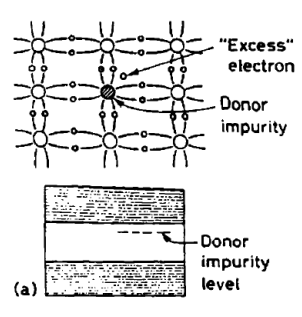
\includegraphics[width=6cm]{semi3.png}
\end{center}

\section{Semiconduttori di tipo p}
Se si sostituisce nel reticolo cristallino un atomo di silicio con un \textit{atomo trivalente (accettore)}, ad esempio un atomo di boro, si forma una lacuna in uno degli atomi vicini, in quanto si creerà nella struttura a bande uno stato addizionale, vicino la banda di valenza. Per effetto dell'agitazione termica uno degli elettroni di valenza degli atomi vicini di silicio può facilmente occupare la lacuna, con la conseguente formazione di una lacuna nella banda di valenza del cristallo di silicio.\\
Un cristallo in cui siano presenti degli accettori ha una conducibilità più elevata assicurata dalle lacune, esso prende il nome di \textit{semiconduttore di tipo p}.\\
Lacune: portatori di carica maggioritari.\\
Elettroni: portatori di carica minoritari.
\begin{center}
    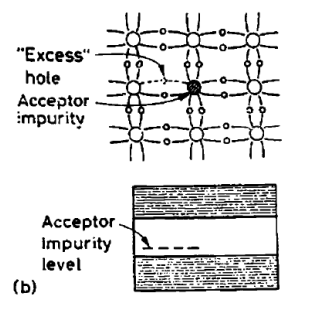
\includegraphics[width=6cm]{semi4.png}
\end{center}

\section{Legge di azione di massa}
Indipendentemente dal tipo drogaggio, la concentrazione di elettroni e lacune obbedisce a una semplice \textit{legge di azione di massa} quando è in equilibrio termico. Se $n$ è la concentrazione di elettroni e $p$ è la concentrazione di lacune, allora il loro prodotto è
$$np=n_i^2=AT^{2/3}\exp\left({\frac{-E_g}{2kT}}\right)$$
dove $n_i$ è la concentrazione intrinseca del semiconduttore.\\
Quindi se aumentano gli elettroni per drogaggio, la quantità delle lacune che si formano normalmente nel semiconduttore non rimane costante ma diminuisce. Analogamente, se aumento le lacune per drogaggio, il numero degli elettroni liberi diminuisce.
Poiché il semiconduttore è neutro, le densità di carica positiva e negativa devono essere uguali, in modo che
$$N_D+p=N_A+n$$
dove $N_D$ e $N_A$ sono la concentrazione, rispettivamente, dei donatori e degli accettori.\\
In un semiconduttore di tipo n, dove $N_A=0$ e $n>>p$, la densità elettronica è quindi
$$n\simeq N_D$$
cioè la concentrazione di elettroni è approssimativamente uguale alla concentrazione del drogante. La concentrazione dei portatori di carica minoritari sarà
$$p=\simeq \frac{n_i^2}{N_D}$$
Da cui avremo che
$$\sigma\simeq eN_D\mu_e$$
Un risultato analogo si trova per i materiali di tipo p.
$$n\simeq\frac{n_i^2}{N_A}~~~\sigma\simeq eN_A\mu_e$$

\section{Semiconduttori di tipo p+, n+, i (compensati)}
I semiconduttori con alte concentrazioni di droganti ($10^{20}$ atomi/cm$^3$, anziché $10^{13}$ atomi/cm$^3$) sono altamente conduttivi. Essi sono indicati con $p+$ e $n+$ e vengono adoperati per creare i contatti elettrici nei semiconduttori.\\
Una domanda che ci si può porre ora è cosa succede se entrambe le impurità di tipo n e p vengono aggiunte a un semiconduttore. In realtà, tutti i semiconduttori contengono impurità di entrambi i tipi. Poiché gli elettroni in più dagli atomi donatori saranno catturati da lacune extra nei materiali accettori, è facile vedere che si verifica un effetto di cancellazione. Ciò che conta, quindi, è la concentrazione netta, $|N_D-N_A|$ , dove $N_D$ e $N_A$ sono le concentrazioni di atomi donatori e accettori. Se $N_D>N_A$, allora il semiconduttore è di tipo n e viceversa. Allo stesso modo, se in un semiconduttore la concentrazione di atomi donatori eguaglia quella degli atomi accettori, il semiconduttori riassume le caratteristiche dei semiconduttori intrinseci.
Questi semiconduttori sono detti \textit{compensati (o di tipo i)} e hanno una resistività elevata, $\sim 100000 \; \Omega cm$.

\section{Giunzioni n-p}
I rivelatori a semiconduttore sono basati in genere sull'utilizzo di una \textit{giunzione n-p}.
Nei rivelatori senza giunzione il rumore di fondo dovuto alla presenza di cariche libere sarebbe infatti troppo elevato. Questo rumore può essere risolto in un volume limitato, sfruttando le proprietà di una giunzione p-n, che consiste nella giunzione fra un semiconduttore di tipo n e uno di tipo p. In effetti, per ottenere un buon contatto su scala atomica, la giunzione viene costruita a partire da un unico pezzo di materiale semiconduttore, le cui estremità opposte vengono drogate una di tipo n e una di tipo p, in modo da ottenere una superficie di separazione il più possibile sottile; oggi si sono raggiunti valori intorno al micron.\\
Nella zona di di giunzione:
\begin{itemize}
    \item Iniziale diffusione di elettroni verso la zona drogata p e di lacune verso la zona drogata n (a causa della differente concentrazione);
    \item Gli elettroni diffusi si ricombinano con le lacune nella zona p, e lo stesso fanno le lacune diffuse nella zona n;
    \item Essendo entrambe le zone n e p inizialmente neutre, nella giunzione la zona n avrà una concentrazione di cariche positive mentre la zona p di cariche negative.
\end{itemize}
Il risultato sarà la creazione di una regione, detta di \textit{svuotamento o di carica spaziale}, in cui non vi sono cariche libere di alcun segno e con un eccesso di ioni negativi (accettori) nella zona p, e di ioni negativi (donatori) nella zona n; tale regione è utile per la rivelazione di radiazione ionizzante. In tale zona si crea un campo elettrico che impedisce ulteriori processi di diffusione $\rightarrow$ Potenziale di contatto $V_0$ (circa 1 V).
\begin{center}
    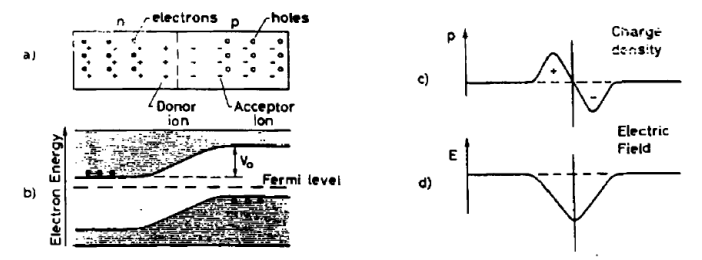
\includegraphics[width=14cm]{semi5.png}
\end{center}
L'ampiezza della zona di svuotamento è generalmente piccola e dipende dalla concentrazione di impurità n e p. Se la distribuzione della densità di carica nella zona, $\rho(x)$ è nota, questa può essere determinata dall'equazione di Poisson.\\
$$\frac{d^2V}{dx^2}=-\frac{\rho(x)}{\varepsilon}$$
dove $\varepsilon$ è la costante dielettrica. Supponendo una distribuzione di densità di carica piatta:
\begin{equation*}
    \rho(x)=
    \begin{cases}
        eN_D & 0<x<x_n \\
        -eN_A & -x_p<x<0 
    \end{cases}
\end{equation*}
Si trova dall’equazione di Poisson:
$$x_n=\bigg( \frac{2\varepsilon V_0}{eN_D(1+N_D/N_A)} \bigg)^{1/2}$$
$$x_p=\bigg( \frac{2\varepsilon V_0}{eN_A(1+N_A/N_D)} \bigg)^{1/2}$$
\begin{center}
    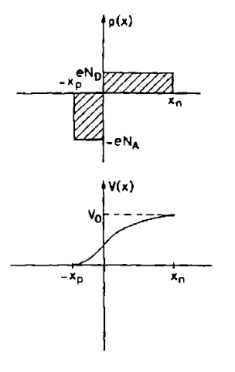
\includegraphics[width=6cm]{semi6.png}
\end{center}
Le dimensioni della regione di svuotamento sono piccole (tipicamente $\sim 100 \mu m$).
In queste condizioni, un rivelatore basato su una giunzione n-p avrà prestazioni scadenti (rumore, risoluzione, stopping power).\\
Applicando una ddp (\textit{polarizzazione inversa}) si allarga la zona di svuotamento, che costituirà il volume sensibile per la rivelazione delle particelle.\\
Lacune ed elettroni sono spazzati via dalla giunzione perché attratti dai rispettivi contatti.\\
La regione di svuotamento può raggiungere anche estensioni pari a mm (limite dettato dalla resistività del materiale).
\begin{center}
    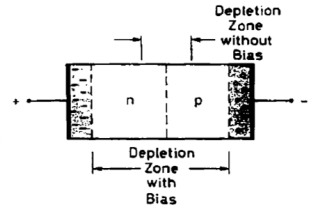
\includegraphics[width=6cm]{semi7.png}
\end{center}

\section{Rivelatori a semiconduttori}
Si basano su una giunzione n-p polarizzata inversamente.\\
Una particella carica che attraversa il dispositivo genera coppie elettrone-lacune. Queste cariche si muovono sotto l’azione del campo elettrico e vengono raccolte dagli elettrodi, dando origine ad un segnale (in modo analogo a quanto avviene per elettroni/ioni in un gas).
\begin{center}
    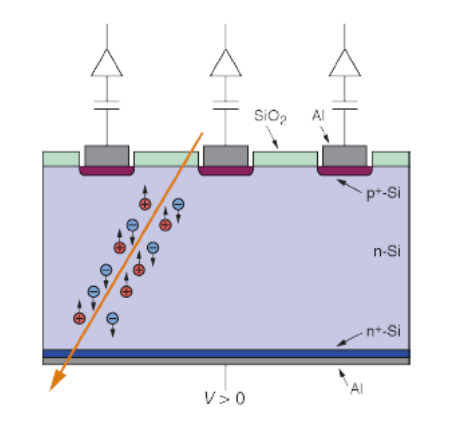
\includegraphics[width=6cm]{rivsemi1.png}
\end{center}
Possiamo immaginarli come l’equivalente a stato solido di una camera a ionizzazione, con un mezzo solido semiconduttore.
\begin{center}
    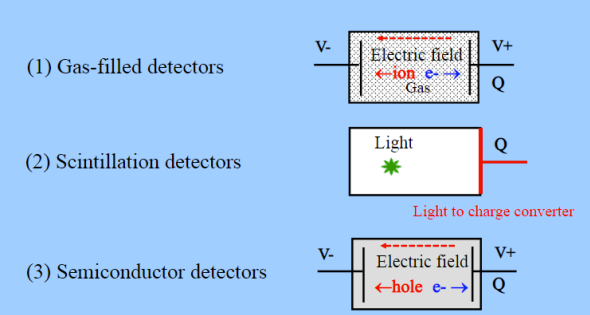
\includegraphics[width=12cm]{rivsemi2.png}
\end{center}
I rivelatori a giunzione possono essere costruiti sfruttando diversi processi per creare la barriera. Tra questi ci sono:
\begin{itemize}
    \item Rivelatori a diffusione;
    \item Rivelatori a barriere superficiale;
    \item Ion-Implanted diodes;
    \item Rivelatori a deriva di Litio.
\end{itemize}

\section{Rivelatori a diffusione}
La superficie del cristallo viene inizialmente levigata e dopo viene depositata su di essa un sottilissimo strato di fosforo. Portando la temperatura tra $700$ e $900^\circ$C il fosforo diffonde nel cristallo per $0.1-1$ micron. Si ottiene così una giunzione molto prossima alla superficie. L'impiego di cristalli di tipo p è dovuto al fatto che con questi è più facile ottenere elevate resistività. Sono però impiegati anche cristalli di silicio di tipo n, con un sottile strato superficiale di tipo p, il quale è meno influenzato da agenti esterni come l'ossigeno e il vapor d'acqua.\\
Il maggiore svantaggio di questi rivelatori è che il processo di diffusione deve avvenire a temperature molto elevate. Questo tende a ridurre la velocità delle cariche formate e quindi ad aumentare il rumore di fondo.\\
Il loro vantaggio sta nella robustezza e nella grande resistenza alle contaminazioni esterne.
\begin{center}
    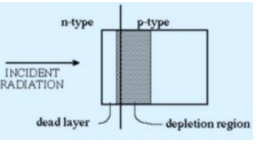
\includegraphics[width=6cm]{semidiff.png}
\end{center}

\section{Rivelatori a barriera superficiale}
In questi rivelatori la barriera è ottenuta facendo ossidare spontaneamente la superficie intaccata chimicamente di un cristallo di silicio di tipo n.\\
Questo processo di ossidazione ha luogo in un periodo di uno o due giorni, trascorso il quale la superficie viene ricoperta con una sottile lamina d'oro ($20-50 mg/cm^2$), ottenuta per evaporazione sotto vuoto. La giunzione è poi montata su un anello isolante con superfici metalliche per assicurare i contatti elettrici.
\begin{center}
    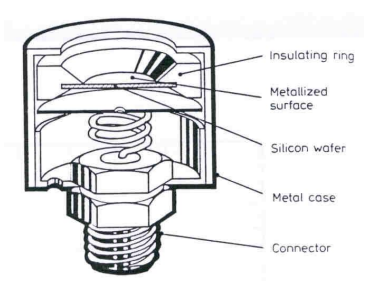
\includegraphics[width=6cm]{semisup2.png}
\end{center}
A causa dei differenti livelli di Fermi dei due materiali la giunzione crea un abbassamento dei livelli delle bande del semiconduttore e ciò è simile a quello che succede in una giunzione p-n e la regione di svuotamento si estende lungo tutto il semiconduttore. Proprio per questo motivo, potendo utilizzare per la rivelazione l'intera regione, alcuni di questi rivelatori vengono costruiti appositamente per misure di $dE$ al passaggio di particelle. Un altro vantaggio è che il processo di lavorazione è a temperatura ambiente (più semplice della diffusione).\\
Uno degli svantaggi di questi rivelatori è la loro sensibilità alla luce. Questo perché il sottile strato di oro è insufficiente a "assorbire" la luce visibile, che avendo una energia di $2-4 eV$ (contro $1,1 eV$ del gap energetico del silicio), produce un segnale di una certa ampiezza che contribuisce all'aumento del rumore di fondo. Un altro è che questi rivelatori sono sensibili alle contaminazioni superficiali.

\section{Ion-Implanted diodes}
Si ottengono bombardando il cristallo semiconduttore con un fascio di ioni (impurità) accelerati con un acceleratore.\\
La concentrazione e il profilo sono determinati dall’energia del fascio.\\
Necessario annealing a $500^\circ$C per il danneggiamento da radiazione.\\
Vantaggi:
\begin{itemize}
    \item Stabili;
    \item Finestre di ingresso sottili (decine di mm).
\end{itemize}
Svantaggi: costosi.

\section{Rivelatori a deriva di litio}
Cercano di risolvere il problema delle piccole dimensioni della regione di svuotamento (limitato dalla resistività del Silicio).\\
Questi tipi di rivelatori sfruttano delle giunzioni p-n più complesse. Infatti in tali rivelatori in un cristallo semiconduttore si realizza oltre ad un drogaggio di tipo n e di tipo p, anche una sottile zona centrale con bassa concentrazione di impurità, zona intrinseca. Si ottiene così quella che viene chiamata \textit{giunzione p-i-n}.\\
Si ottengono attraverso la diffusione di Litio (donatori) in un semiconduttore di tipo p. Attraverso l’applicazione di una ddp e aumentando la temperatura il Litio si propaga nella zona p creando una zona compensata di spessore $10-15 mm$.
\begin{center}
    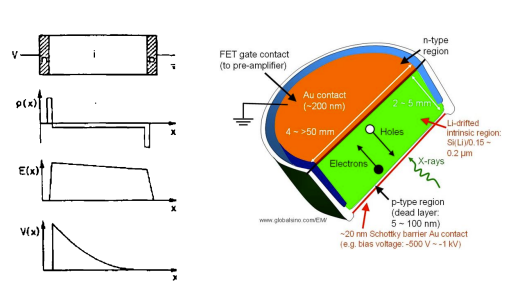
\includegraphics[width=9cm]{semilitio.png}
    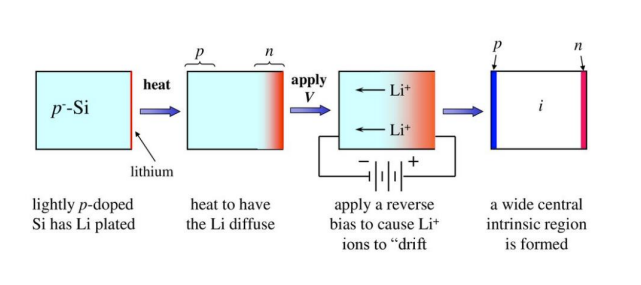
\includegraphics[width=12cm]{semilitio2.png}
\end{center}
Vantaggi:
\begin{itemize}
    \item Spessori elevati (spettroscopia beta e raggi x a bassa energia).
\end{itemize}
Svantaggi:
\begin{itemize}
    \item Utilizzo a basse temperature (a causa dell’elevato rumore termico);
    \item Conservazione a basse temperature per mantenere la zona intrinseca.
\end{itemize}

\section{Realizzazione dei contatti}
Contatti Ohmici non possono essere realizzati dalla semplice deposizione di metallo sul semiconduttore (poiché di creerebbe una giunzione).\\
È necessario interporre uno strato $p+$ e $n+$ tra il semiconduttore e il metallo.
\begin{center}
    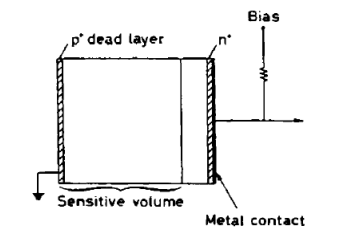
\includegraphics[width=6cm]{semi_contatto.png}
\end{center}

\newpage
\section{Caratteristiche dei rivelatori a semiconduttore}
\section{Linearità}
Supponendo che la regione di svuotamento sia sufficientemente spessa da fermare completamente tutte le particelle, la risposta dei semiconduttori dovrebbe essere perfettamente lineare con l'energia.
$$V=\frac{Q}{C}=\eta\frac{E}{wC}$$
dove $\eta$ è l'efficienza di raccolta delle cariche e $w$ è l'energia media.\\
Inoltre, poiché $w$ è indipendente dal tipo di particella, la risposta è, in linea di principio, anche indipendente dal tipo di radiazione. Questo risulta essere vero solo per radiazioni leggermente ionizzanti come elettroni e protoni. Per gli ioni più pesanti, non è così a causa di effeti di plasma.\\
Se la zona di svuotamento non è sufficientemente spessa verrà misurata la perdita di 
energia (non lineare con l’energia delle particelle).

\section{Risoluzione in energia}
La risoluzione energetica intrinseca dipende dal numero di portatori di carica e dal fattore Fano. Nonostante numerosi esperimenti, il fattore Fano sia per il silicio che per il germanio non è ancora ben determinato. Tuttavia, è chiaro che F è piccolo e dell'ordine di 0,12.\\
Ciò, ovviamente, contribuisce notevolmente a migliorare la risoluzione dei semiconduttori che già beneficiano notevolmente della piccola energia media richiesta per creare una coppia di lacuna-elettrone.
La risoluzione è pari a:
$$R=2.35\sqrt{\frac{Fw}{E}}$$
Per $E=5$ MeV e $f\sim 0.12$ la risoluzione intrinseca è $0.07\%$, cioè $3.5$ KeV.\\
A parità di energia depositata, il n. di coppie elettrone-lacuna è 10 volte maggiore che nei gas. La risoluzione è circa 3 volte maggiore ai rivelatori a gas.

\section{Sensibilità ed efficienza intrinseca}
Per le particelle cariche, l'\textit{efficienza di rilevamento intrinseca} dei semiconduttori è prossima al $100\%$. I fattori limitanti sono le correnti di dispersione e l'elettronica che impongono una soglia minima sul segnale da rivelare. Infatti, per garantire un segnale adeguato, la zona di svuotamento deve essere scelta sufficientemente spessa in modo tale da produrre una ionizzazione sufficiente per formare un segnale più grande del livello di rumore.\\
Allo stesso modo la presenza di una zona morta prima del volume sensibile introduce una soglia in energia (circa $10 KeV$ per alfa da $5 MeV$).

\newpage
\section{Densità}
L'elevata densità comporta:
\begin{itemize}
    \item grande perdita di energia su distanze piccole;
    \item la diffusione è minore rispetto ad un rivelatore a gas, il che si traduce in migliori prestazioni in termini di risoluzione spaziale.
\end{itemize}

\section{Tempo di risposta}
Il tempo di raccolta per elettroni e lacune dipende dal punto in cui si trovano le cariche rispetto agli elettrodi.\\
Il segnale elettrico agli elettrodi deriva dall’induzione causata dal movimento delle cariche (piuttosto che dalla reale raccolta).\\
I rivelatori a semiconduttore sono molto veloci (impulsi con tempi di salita di alcuni ns).

\section{Danneggiamento da radiazione}
I rivelatori a semiconduttore, specialmente quelli sviluppati per operare in esperimenti di Fisica delle Alte Energie, devono essere progettati e testati per poter sopravvivere agli alti livelli di radiazione cui saranno esposti durante il loro funzionamento.\\
La radiazione può provocare diversi effetti: Bulk e Surface.
\section{Effetti sul bulk}
Silicio: Danno sul reticolo (bulk damage, displacement damage) dovuto a Non Ionizing Energy Loss (NIEL) (p, n, $\pi$).
Cambio della tensione di svuotamento (maggiori tensioni operative, svuotamento non totale). Aumento della corrente di leakage (cooling).
Diminuzione dell’efficienza di raccolta della carica (charge collectionefficiency, CCE).

\section{Effetti sulla superficie}
Ossido: danno superficiale dovuto a Ionizing Energy Loss (IEL).\\
Dovuto all'accumulo di cariche positive all'interno degli ossidi ($SiO_2$) o all'interfaccia $Si/SiO_2$.\\
Può influire sul noise, sul breakdown.

\section{Effetti cumulativi}
Sono i danni che irrimediabilmente si accumulano con l’esposizione prolungata alla radiazione.\\
Questi danni sono prevedibili in laboratorio e ci permettono di stabilire una vita media utile per ogni dispositivo:
\begin{itemize}
    \item Total Ionizing Dose (TID);
    \item Displacement Damage (DD).
\end{itemize}

\section{Single Event Effects (SEE)}
Sono imprevedibili e possono apparire in qualsiasi momento. Si raggruppano in due categorie: gli effetti transitori (o soft error), come il Single Event Transient(SET) e il Single Event Upset(SEU); gli effetti catastrofici permanenti come il Single Event Gate Rupture (SEGR).
\section{Danneggiamento da radiazione: Effetti e Applicazioni} % Titolo aggiunto per la sezione vuota
Gli effetti di danneggiamento dipendono dalla dose depositata (Dose = Energia/massa [Gray = J/kg]) e dal tipo di particella.\\
\textbf{Esempio}: presso LHC, collisioni tra protoni (a 14 TeV) e tra ioni pesanti (a 5.5 TeV/A) danno luogo alla produzione di un enorme numero di particelle che attraversano i rivelatori al Silicio dei vari esperimenti!
$$l_{max}\sim 10^{34} cm^{-2} s^{-1}$$
ad una distanza di 4 cm $\sim 3 \times 10^{15} \text{ (neq) } cm^{-2}$
in 10 anni ($>85\%$ adroni carichi).\\
\textbf{! DANNEGGIAMENTO DA RADIAZIONE !}

\section{Applicazioni nella spettroscopia di particelle cariche}
A causa delle loro proprietà (risoluzione, timing,...) sono molto usati nella spettroscopia di particelle cariche.\\
Singoli rivelatori disponibili in un’ampia varietà di spessori (da pochi micron a 5000 micron) e di area sensibile (da pochi $mm^2$ ad alcuni $cm^2$).\\
Sensibili con efficienza $100\%$ a protoni, particelle alfa e ioni pesanti. Spessore da valutare in base al tipo di particella da rivelare e al range.\\
Per elettroni, lo spessore dei rivelatori disponibili è in genere troppo piccolo per poterli arrestare.

\section{Alcuni sviluppi moderni}
Nei grandi rivelatori per la fisica delle alte energie l’uso dei rivelatori al silicio è aumentato sempre più negli ultimi decenni, soprattutto a causa della riduzione dei costi di produzione e dell'avvento della microelettronica.\\
Nella maggior parte dei casi i rivelatori sono attraversati dalle particelle (di alta energia), da cui la necessità di avere spessori piccoli (per non disturbare le traiettorie delle particelle).\\
Oggi quasi tutti gli esperimenti di alta energia e nello spazio usano ampiamente i rivelatori al silicio.

\newpage
\section{Tipologie moderne di rivelatori al silicio}
Le versioni recenti di rivelatori al silicio sfruttano le buone capacità di tracciamento (risoluzione spaziale) e risoluzione energetica.\\
Due possibili scelte:
\begin{itemize}
    \item \textit{Readout continuo}: rivelatori a drift al silicio (silicon drift);
    \item \textit{Readout discreto}: rivelatori a pixel e a microstrip.
\end{itemize}

\section{Rivelatori a microstrip}
\begin{itemize}
    \item Elettrodi di lettura costituiti da strip a distanza di decine di micron;
    \item Il segnale è indotto su una o più strip contigue;
    \item 1D info (baricentro) → 2 strati per ottenere 2D info oppure strip su entrambi i lati;
    \item Tensione 160 V per uno svuotamento completo 100 coppie $e-h/\mu m \rightarrow$ 30 000 coppie;
    \item Risoluzione spaziale $\sim 5 \mu m$;
    \item Tempi di raccolta delle cariche $\sim 10$ ns;
    \item Ambiguità nella ricostruzione della posizione.
\end{itemize}
\begin{center}
    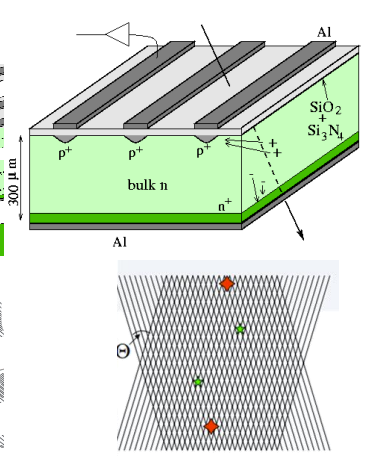
\includegraphics[width=8cm]{microstrip.png}
\end{center}

\section{Rivelatori a drift}
Analoghi alle camere a deriva a gas:
\begin{itemize}
    \item elettroni derivano all’interno del rivelatore e sono raccolti da un elettrodo segmentato $\implies$ anodi ($\sim \mu s$);
    \item 2 coordinate spaziali $\implies$ anodi e tempo di deriva;
    \item campo elettrico di deriva uniforme e generato con elettrodi opportuni.
\end{itemize}
Sistema di lettura dati molto meno complesso di microstrip e pixel.\\
Nessuna ambiguità nella ricostruzione della posizione.\\
Rivelatori lenti che necessitano di temperature stabili.
\begin{center}
    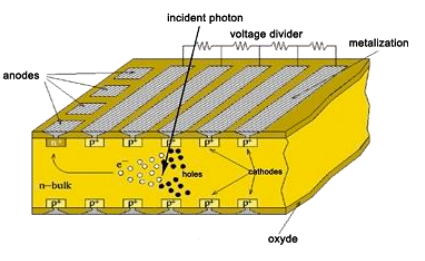
\includegraphics[width=8cm]{drift.png}
\end{center}



\section{CCD (Charged-Coupled Device)}
Matrice bidimensionale fino a $\approx 10^6$  pixel/$cm^2$ (pixel $\sim 10 \times 10 \mu m^2$).
\begin{center}
    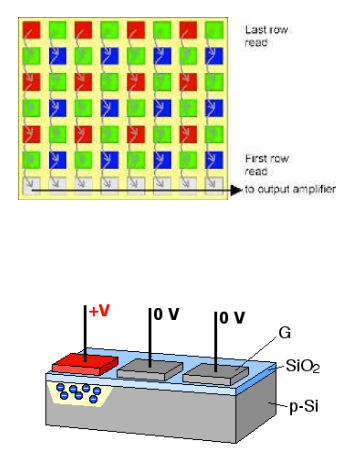
\includegraphics[width=6cm]{ccd.png}
\end{center}
Funzionamento:
\begin{itemize}
    \item particella ionizzante $\rightarrow$ coppie e-h $\rightarrow$ $h^+$ si muovono verso gli elettrodi p mentre gli $e^-$ sono confinati in corrispondenza del minimo di potenziale negativo (energia potenziale);
    \item la carica di ionizzazione confinata in un pixel è spostata al successivo mediante un potenziale variabile periodico, senza perdita di $e^-$;
    \item la nube di $e^-$ raggiunge l’ultima cella dove è rivelata.
\end{itemize}
Caratteristiche:
\begin{itemize}
    \item 2D detector $\implies$ informazione relative ad entrambe le coordinate spaziali, senza ambiguità (accuratezza spaziale $\approx 10 \mu m$);
    \item tempi di lettura molto lunghi $\approx 10 msec \implies$ impiego limitato in esperimenti di fisica delle alte energie $\implies$ pile up!
    \item buona risoluzione energetica e spaziale $\implies$ utilizzati per videocamere e in astronomia per spettroscopia di raggi X.
\end{itemize}

\section{Rivelatori a pixel}
I rivelatori a pixel sono matrici di singoli rivelatori corredate della opportuna elettronica montata a stretto contatto con il rivelatore.\\
La cella (o le celle) colpite indicano la posizione $(X,Y)$ relativa al passaggio della traccia, con risoluzioni dell’ordine della decina di micron.\\
Vantaggi:
\begin{itemize}
    \item 2D $\mu-$detector;
    \item piccole dimensioni: $50 \mu m \times 50 \mu m$;
    \item basso livello di rumore (bassa capacità) e buon rapporto $S/N$;
    \item rivelatori veloci;
    \item adatti per alte densità di particelle.
\end{itemize}
Svantaggi
\begin{itemize}
    \item elevato numero di canali;
    \item elevato numero di connessioni elettriche;
    \item grande dispersione di potenza;
    \item molto fragile;
    \item tecnologia all'avanguardia.
\end{itemize}

\section{Problema: collegare il circuito di amplificazione a ciascun pixel}
\section{Rivelatori ibridi (bump bonding)}
Rivelatore e chip di lettura sono due oggetti fisicamente distinti e sono posizionati uno sopra l’altro. I bump-bond formano la connessione elettrica fra ciascun pixel e la sua elettronica.\\
Il bump-bonding è un limite per questi oggetti: 
\begin{itemize}
    \item è un processo costoso;
    \item limita le dimensioni del pixel;
    \item introduce problemi di material budget (multiple scattering).
\end{itemize}
\begin{center}
    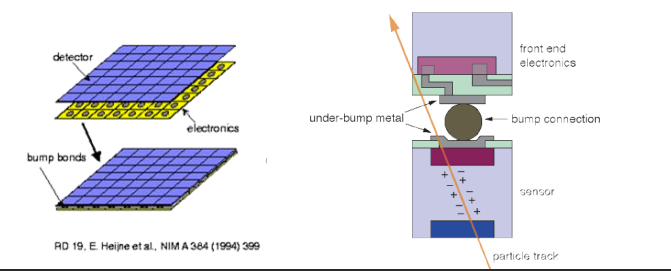
\includegraphics[width=\linewidth]{pixel.png}
\end{center}

\section{Rivelatori monolitici (MAPS: Monolithic Active Pixel Sensors)}
Elettronica integrata sullo stesso sensore, no bonding.
\begin{itemize}
    \item processo commerciale;
    \item design relativamente semplice;
    \item la carica generata in uno strato di $15-20 \mu m$ di Silicio epitassiale (elettroni) viene raccolta da un elettrodo n per diffusione;
    \item non sono necessarie connessioni elettriche;
    \item è possibile diminuire le dimensioni dei pixel;
    \item più sensibili al danno da radiazione.
\end{itemize}
\begin{center}
    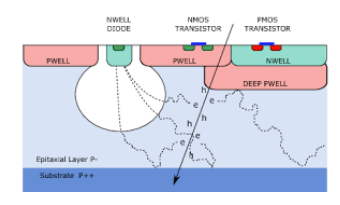
\includegraphics[width=11cm]{pixel2.png}
\end{center}

















\chapter{La tecnologia del vuoto}
\section{Un po' di storia}
\begin{itemize}
    \item Concetto di vuoto introdotto per la prima volta da Democrito nella teoria atomista della materia.
    \item Galileo studiò il vuoto sperimentalmente attraverso una pompa aspirante;
    \item 1644 primo barometro a mercurio (Torricelli);
    \item 1654 prima pompa da vuoto e spettacolare dimostrazione con le sfere di Magdeburgo (Von Guericke);
    \item 1850 primo vacuometro (McLeod);
    \item 1905 prima pompa rotativa a mercurio (Gaede).
\end{itemize}

\section{Il vuoto}
Nel linguaggio scientifico il termine \textit{vuoto} viene usato con due accezioni:
\begin{itemize}
    \item spazio totalmente privo di materia;
    \item regione di spazio occupata da aeriformi con pressione sostanzialmente inferiore a quella atmosferica (pressione del gas $<<$ pressione atmosferica).
\end{itemize}
L'unità di misura della pressione stabilita dal sistema internazionale di misura è il Pascal:
$$1 ~ Pascal~=1\frac{N}{m^2}$$
La \textit{pressione atmosferica} è la pressione presente in qualsiasi punto dell'atmosfera terreste e si definisce come il rapporto tra il peso esercitato da una colonna d'aria e l'unità di superficie su cui esso agisce. Nella maggior parte dei casi, infatti, il valore della pressione atmosferica è equivalente a quello della pressione idrostatica esercitata dal peso dell'aria presente al di sopra del punto di misura.\\
La pressione atmosferica è funzione dell'altezza, della latitudine, della temperatura e dell'umidità.
Nel grafico sottostante rappresenta la pressione in funzione dell'altitudine.
\begin{center}
    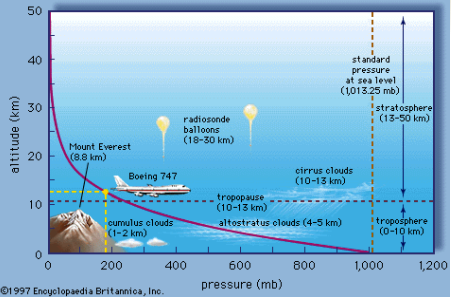
\includegraphics[width=8cm]{vuoto1.png}
\end{center}
Il luogo dei punti dell'atmosfera in cui la pressione è in un
dato istante, costante costituisce una superficie isobara.\\
All'aumentare della temperatura l'aria si dilata, diminuisce la
sua densità e di conseguenza in generale una colonna d'aria
calda peserà meno di una uguale colonna di aria fredda.\\
Il grafico sottostante rappresenta variazioni della pressione atmosferica (periodiche, dovute al ciclo giorno-notte) e aperiodiche (dovute alle condizioni complessive meteo).
\begin{center}
    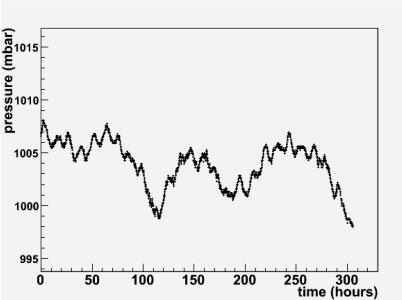
\includegraphics[width=6cm]{vuoto2.png}
\end{center}
Le variazioni giornaliere di pressione vanno attribuite alle maree atmosferiche e all'espansione dell'aria che accompagna l'aumento di temperatura causato dalla radiazione solare.\\
Si assume come valore della pressione atmosferica normale o standard quella misurata alla latitudine di $45^\circ$, al livello del mare e ad una temperatura di $15 ^\circ C$, che corrisponde ad una colonna di mercurio di $760 mm$.\\
La misura del vuoto si riconduce quindi alla misura della pressione che un gas presenta rispetto alla pressione atmosferica. Quest'ultima viene pertanto assunta come valore limite superiore. \textit{Più il vuoto è “buono” più piccolo è il suo valore di pressione rispetto a quello atmosferico}.\\
Sulla superficie lunare si ha la presenza di gas come $H^2, He, Ne, Ar$ ad una pressione totale intorno ai $10^{-6}~Pa ~(10^{-8}~ mbar)$.\\
Nello spazio interstellare la pressione è ancora più piccola tanto che si preferisce parlare di numero di atomi o molecole per $cm^3$ o $m^3$
Artificialmente è possibile ricreare il vuoto per mezzo di pompe di vario genere.

\section{Tecnologie del vuoto}
La tecnologia del vuoto ha permesso di:
\begin{itemize}
    \item Osservare nuovi fenomeni (es. effetto fotoelettrico);
    \item Sviluppare nuove tecniche di analisi (es. spettroscopia di massa);
    \item  Costruire macchinari d'indagine.
\end{itemize}
Oggi grazie alle nuove tecnologie si raggiungono:
\begin{itemize}
    \item $10^{-9}$ mbar (1 Atmosfera $\sim 10^3$ mbar) $\rightarrow$ acceleratori;
    \item $10^{-12}$ mbar (confrontabili con quelle presenti nello spazio siderale) su piccoli volumi ($< 0.1 m^3$) $\rightarrow$ ricerca sui materiali.
\end{itemize}
Il vuoto è indispensabile per molte applicazioni ed è quindi necessario produrlo in ambienti o recipienti adatti attraverso opportuni dispositivi.
Le applicazioni, in campo scientifico, sono:
\begin{itemize}
    \item Esperimenti in cui studiamo particelle che si muovono libere (in un acceleratore) o che vengono utilizzate come sonda per studiare la materia dobbiamo minimizzare la probabilità di interazione con l’atmosfera circostante;
    \item Esperimenti della materia condensata in cui si studiano superfici e in generale pochi strati atomici della materia;
    \item Simulare particolari situazioni fisiche come quelle che si verificano nello spazio planetario (camere di simulazione spaziale per prove su satelliti e navi spaziali);
    \item Controllare la pressione del gas in esame (per es. riduzioni di $O_2, H_2O$ e idrocarburi in tubi elettronici o in sistemi in cui si studia la scarica nei gas).
\end{itemize}
Le applicazioni, in campo tecnologico, sono:
\begin{itemize}
    \item Isolamento termico creando delle intercapedini in cui è viene creato il vuoto (per es. nei dewars, i contenitori dei liquidi freddi);
    \item Rallentare i processi di decomposizione organica dovuti ad agenti aerobici (es. materiale organico sotto vuoto);
    \item Impedire processi chimico-fisici causati dall’azione dei gas atmosferici (es. evitare cariche nel gas e reazioni chimiche sul filamento in tubi termoionici o durante la fusione di particolari metalli reattivi);
    \item Eliminare gas disciolti contenuti in un dato materiale (es. liofilizzazione).
\end{itemize}
Si definisce \textit{grado di vuoto} la rarefazione ottenuta nel recipiente da evacuare, che viene misurata dalla pressione assoluta dei gas residui.
\begin{center}
    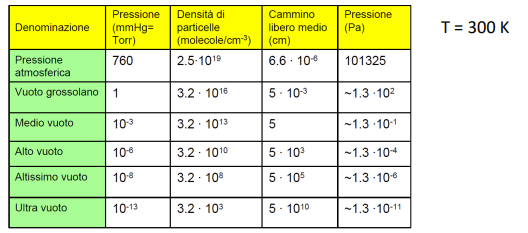
\includegraphics[width=14cm]{vuoto3.png}
\end{center}
\section{Sistemi da vuoto}
Un sistema da vuoto è costituito da quattro tipi di componenti:
\begin{enumerate}
    \item Una camera a vuoto;
    \item Un impianto di pompaggio;
    \item Un apparato di misura del vuoto;
    \item Un complesso di giunti, valvole, condotti e trappole che richiede l’uso di particolari guarnizioni e materiali per vuoto.
\end{enumerate}
\begin{center}
    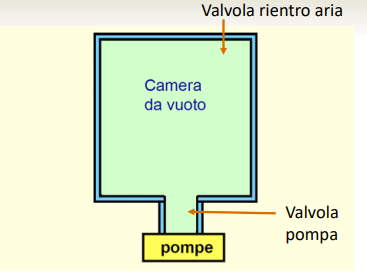
\includegraphics[width=6cm]{vuoto4.png}
\end{center}
Il sistema a vuoto può essere di due tipi: sigillato e pompaggio continuo. Il primo è un vuoto statico, mentre il secondo è un vuoto dinamico, si mantiene un valore costante di vuoto tramite l'aspirazione dell'aria.
\begin{center}
    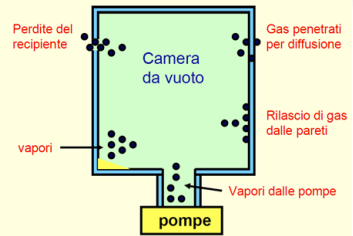
\includegraphics[width=6cm]{vuoto5.png}
\end{center}
In generale, in ogni sistema a vuoto si ha una serie di processi che comportano il rilascio di un certo flusso di gas all'interno della camera a vuoto. Questi gas devono venire in qualche modo eliminati se si vuole che il vuoto si mantenga al grado iniziale.
\'E utile definire due grandezze:
\begin{itemize}
    \item Portata volumetrica $\Sigma$: è detta anche velocità di pompaggio 
    $$\Sigma=\frac{dV}{dt} (m^3s^{-1})$$ 
    è la variazione di volume per unità di tempo, in altre parole la quantità di volume di gas aspirata in un secondo;
    \item Portata $Q$: è il prodotto tra la pressione e la portata volumetrica.
    $$Q=\Sigma P (m^3 Pa s^{-1})$$
\end{itemize}


\section{Evoluzione della pressione nel tempo in un recipiente ideale (privo di perdite)}
Consideriamo un recipiente ideale a pareti rigide di volume V contenente N molecole di gas alla temperatura T ed alla pressione P. Il recipiente è collegato ad una pompa da vuoto tramite un condotto di sezione A (A è la sezione del foro che collega il recipiente al condotto).
$$-V\frac{dP}{dt}=P\Sigma= P \frac{dV}{dt}$$
Se $\Sigma=const$ allora si ha
$$P(t)=P_0e^{-t/\tau}$$
con $\tau=\frac{V}{\Sigma}$, la pressione diminuisce in modo esponenziale decrescente.
\begin{center}
    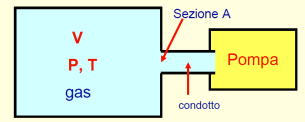
\includegraphics[width=6cm]{vuoto6.png}
\end{center}

\section{Evoluzione della pressione nel tempo in un recipiente con perdite}
Supponiamo che:
\begin{itemize}
    \item il recipiente presenti delle perdite;
    \item alcune molecole si "staccano" dalla superficie del recipiente;
    \item sono presenti dei vapori che derivano dalla pompa stessa.
\end{itemize}
Questo equivale a considerare una portata $Q_F$ di molecole che ha verso opposto al flusso di molecole aspirate $Q_A$, in quanto questo flusso va verso l'interno del contenitore e non verso l'esterno.
$$-V\frac{dP}{dt}=P\Sigma-Q_F$$
Per trovare la \textit{pressione limite}, che dipende dal recipiente, consideriamo il sistema a \textit{regime stazionario} (tante molecole vengono aspirate dalla pompa e tante ne vengono immesse nel recipiente dalle varie perdite):
$$P_{lim}=\frac{Q_F}{\Sigma}$$

\section{Legge di Ohm del vuoto}
Consideriamo un recipiente da svuotare che ha la pressione $P$, connesso, tramite un 
condotto di conduttanza $C$, ad una pompa ideale che alla pressione di lavoro $P_P$ ha al suo 
ingresso una velocità di aspirazione $\Sigma P$. 
\begin{center}
    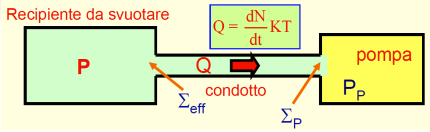
\includegraphics[width=9cm]{vuoto7.png}
\end{center}
Vogliamo ricavare la velocità di pompaggio 
efficace $\Sigma_{eff}$ all'ingresso del recipiente.
$$Q=C\Delta P \implies \frac{1}{\Sigma_{eff}}=\frac{1}{C}+\frac{1}{\Sigma_P}$$
La conduttanza della connessione riduce l’effettiva portata della pompa.

\section{Fluidodinamica-Elettricità}
\begin{center}
    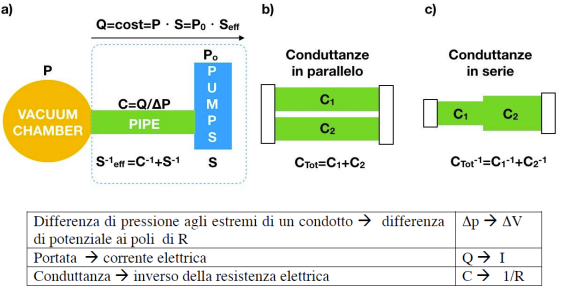
\includegraphics[width=14cm]{flu_ele.png}
\end{center}

\section{Pompe a vuoto}
Per evacuare una recipiente qualsiasi del fluido in esso contenuto, occorre stabilire una differenza di pressione tra il contenitore che si vuole vuotare ed un’altra regione di spazio.\\
Le pompe da vuoto sono dei dispositivi aspiranti destinate a vuotare recipienti chiusi contenenti del fluido.\\
Le pompe a vuoto possono essere:
\begin{itemize}
    \item \textit{Meccaniche}: il funzionamento di questo tipo di pompe si basa sul movimento di organi meccanici. La pressione limitenon è molto bassa dato che necessariamente le parti in movimento non possono avere una tenuta perfetta (rotativa,turbomolecolare);
    \item \textit{A getto d'acqua};
    \item \textit{A vapore};
    \item \textit{Criogeniche};
    \item \textit{Ioniche}.
\end{itemize}
Ogni tipologia di pompa può coprire un intervallo differente di pressione.
\begin{center}
    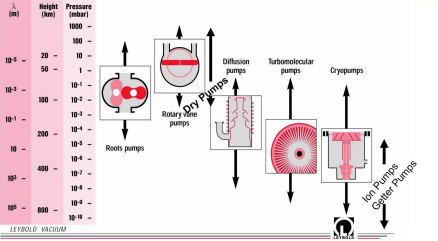
\includegraphics[width=14cm]{pompa1.png}
\end{center}
Ogni tipo di pompa è caratterizzato dai valori della velocità di pompaggio e della pressione limite (che dipende dalla pressione all’ingresso della pompa).\\
Si deve tener conto che tanto più è bassa la pressione che si vuole raggiungere tanto più la pressione di partenza è minore della pressione atmosferica.

\section{Pompe meccaniche: pompa rotativa}
Le pompe meccaniche sono comunemente usate per produrre il vuoto primario (basso e medio vuoto) partendo dalla pressione atmosferica.\\
Una pompa rotativa è un tipo particolare di pompa a vuoto di tipo meccanico.\\
Il principio di funzionamento è relativamente semplice: si tratta di mettere in comunicazione con l'ambiente nel quale si intende fare il vuoto una zona a bassa pressione, che viene quindi riempita con il gas da espellere. Successivamente, quella regione viene scollegata  dall'ambiente e infine svuotata all'esterno. Il tutto procede ciclicamente grazie all'uso di meccanismi rotanti a tenuta.\\
Vi sono due tipi di pompe: a palette ed a pisone rotante.

\section{Pompa rotativa a palette}
La \textit{pompa rotativa a palette} è costituita da un rotore provvisto di palette mobili che ruota eccentricamente in una cavità cilindrica connessa al condotto di ingresso e di uscita.
\begin{center}
    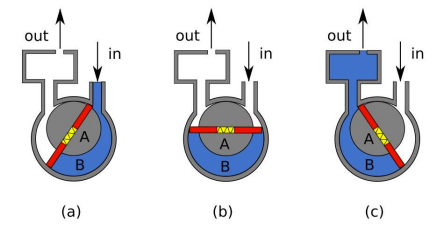
\includegraphics[width=8cm]{pompa2.png}
\end{center}
Le palette vengono tenute a contatto con la superficie interna dello statore da una molla e dalla forza centrifuga. Tra le palette e lo statore è sempre presente un velo d'olio come elemento di tenuta. La variazione di volume delle camere crea depressioni (fase di aspirazione) e compressioni dell'aria (fase di scarico). Nella fase di aspirazione il gas viene estratto dalla camera da vuoto tramite il manicotto di aspirazione, successivamente grazie all'eccentricità del rotore la camera continua ad aumentare di volume. Una volta raggiunto il volume massimo il manicotto di aspirazione viene chiuso da una seconda paletta mentre la camera della pompa comincia a diminuire di volume consentendo ai gas di essere espulsi dal manicotto di scarico.\\
Tramite questa tipologia di pompe si possono raggiungere pressione finali dell'ordine $10^{-2}-10^{-3}$ mbar.\\
Le pompe rotative di questo tipo sono molto robuste e poco costose, scaricano direttamente in atmosfera e non si verificano fenomeni di saturazione. Nonostante ciò posso comunque verificarsi episodi di retro diffusione dell'olio verso il sistema da vuoto, è necessaria la presenza di trappole che blocchino i vapori d'olio, in caso di gas reattivi l'olio può danneggiarsi e infine il vuoto limite è dell'ordine di $10^{-2}$ Pa.

\section{Pompa rotativa a pistone rotante}
La \textit{pompa a pistone rotante} è concepita per raggiungere velocità di pompaggio ancora più elevata (quindi 
pressioni finali più basse). \\
L’albero di rotazione del rotore è coassiale rispetto alla cavità cilindrica mentre il corpo del rotore (camma) è eccentrico rispetto all’albero.
Un pistone cavo trascinato dalla cammaeccentrica pone in comunicazione il recipiente da evacuare con la cavità cilindrica.\\
Il rotore durante il suo moto comprime i gas fino ad
espellerli nell’atmosfera attraverso la valvola di
scarico.
\begin{center}
    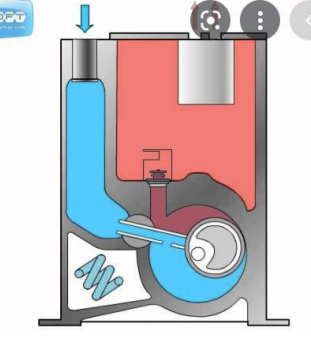
\includegraphics[width=5cm]{pompa3.png}
\end{center}

\section{Pompe meccaniche: pompa a membrana}
La \textit{pompa a membrana}, detta anche a diaframma, è un tipo di pompa a vuoto che sfrutta le variazioni alternate del volume di una camera (espansione e contrazione) per 
generare disequilibri di pressione tra la camera e gli spazi contigui.\\
L'espansione e la contrazione sono generate per mezzo delle oscillazioni alternate di un elemento elastico, chiamato appunto membrana. Il movimento può essere impresso alla membrana per via meccanica, per esempio attraverso un sistema a leva oppure pneumaticamente, alternativamente introducendo e rilasciando aria compressa in una camera opposta a quella di pompaggio.\\
La pressione massima è limitata dalla resistenza del materiale, solitamente gomma.\\
Il vuoto che si realizza è esente da idrocarburi, può scaricare in atmosfera, il funzionamento è reversibile ed il tutto è impermeabile. Il vuoto che riesce a produrre tuttavia è basso e la velocità di pompaggio è limitata.
\begin{center}
    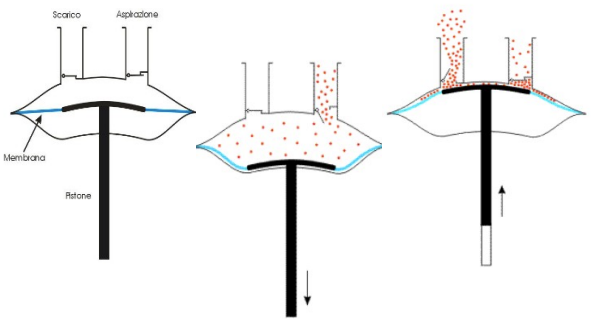
\includegraphics[width=8cm]{pompa4.png}
\end{center}

\section{Pompe filtro a senso unico: pompa a diffusione}
La \textit{pompa a diffusione} è una pompa per l'alto vuoto priva di parti in movimento, essa è in grado di generare una pressione inferiore a $10^{-5}$ mbar, il suo funzionamento è basato sulla diffusione dei vapori di un olio a bassissima tensione di vapore.\\
La pompa è costituita da un recipiente inferiore che contiene l'olio e il sistema di riscaldamento, dal quale si diparte un condotto verticale che termina con una serie di ugelli rivolti verso il basso; il tutto è contenuto in un recipiente collegato ad una camera, dove si fa il vuoto, e con una pompa ausiliaria a medio vuoto. I vapori di olio salgono nel condotto e fuoriescono ad alta velocità dagli ugelli, trascinando le molecole di gas verso la zona del recipiente inferiore, o detto fornello, dove queste sono aspirate dalla pompa ausiliaria. I condotti di collegamento con la camera e con la pompa ausiliaria sono muniti di diaframmi e raffreddati, così da far condensare i vapori d'olio evitandone la fuoriuscita.\\
Le pompe a diffusione sono affidabili e richiedono una manutenzione assai limitata.\\
I vantaggi dell'utilizzo di pompe a diffusione sono l'assenza di saturazione, la velocità di pompaggio poco dipendente dalla natura del gas, la robustezza e la facilità di manutenzione, l'assenza di campi elettrici e magnetici elevati e il costo di acquisto e manutenzione relativamente modesto.


\section{Pompe filtro a senso unico: pompa turbomolecolare}
Le pompe turbo molecolari sono disponibili commercialmente dalla fine degli anni 50\textquotesingle.\\
Per il loro funzionamento è necessario disporre di una pompa meccanica primaria ($10^{-3}$ mbar) e si ottengono pressioni finali dell’ordine di $10^{-9}$ mbar.\\
Le molecole dei gas sono trascinate verso la bocca di evacuazione da un sistema di palette opportunamente distanziate ed inclinate e poste in rapidissima rotazione all’interno di una cavità cilindrica.\\
Nelle pompe turbomolecolari moderne la velocità di rotazione delle palette è di decine di migliaia di giri al minuto e la velocità periferica raggiunge centinaia di metri al secondo.
I vantaggi sono l'eliminazione dei gas pompati verso l'esterno
senza particolari problemi di saturazione, l'assenza di fluidi
motori (quindi pompaggio pulito) e la semplice manutenzione.\\
Gli inconvenienti sono la necessità di un pompaggio
preliminare, una struttura meccanica delicata , un costo di
acquisizione elevato e la raggiunta di un voto limite di $10^{-7}-10^{-8}$ Pa dovuto allo scarso pompaggio di $He$ e $H_2$.
\begin{center}
    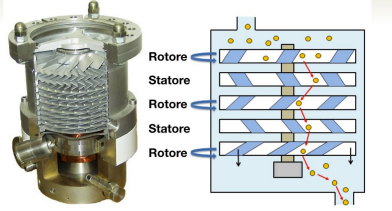
\includegraphics[width=7cm]{pompa6.png}
\end{center}

\section{Misura della pressione negli impianti da vuoto}
Gli strumenti che misurano direttamente la pressione, sono detti genericamente \textit{manometri} (assoluti o differenziali).\\
I manometri assoluti che misurano la pressione nell’intorno di quella tipica dell’atmosfera terrestre sono detti \textit{barometri}.\\
Gli strumenti che misurano pressioni inferiori a quella atmosferica sono denominati \textit{vacuometri}. I vacuometri sono strumenti di natura diversa che sono in grado di coprire un intervallo di 17 ordini di grandezza sfruttando differenti proprietà dei gas rarefatti (accuratezza $\pm10\%$, risposta veloce).\\
Lo strumento di misura risulta tanto più complesso quanto più il gas è rarefatto.\\
I vacuometri possono essere raggruppati sia sulla base dell’intervallo di pressione in cui operano, sia secondo il criterio del principio fisico su cui si base lo strumento.
\begin{center}
    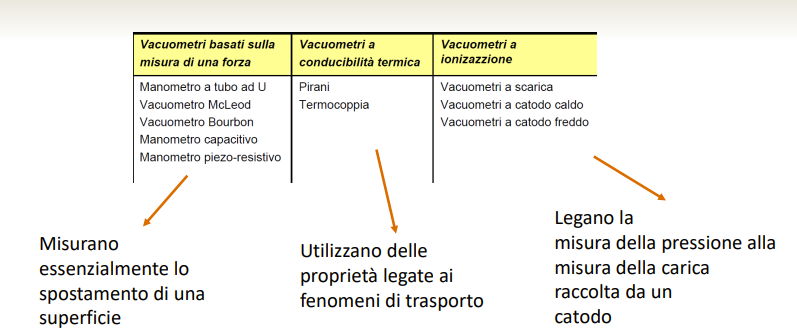
\includegraphics[width=\linewidth]{pompa7.png}
\end{center}

\begin{center}
    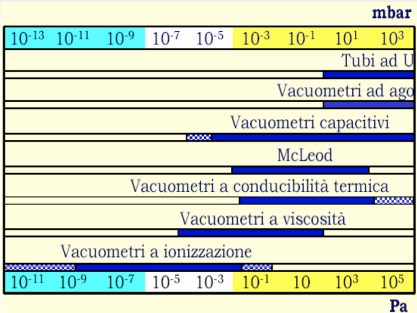
\includegraphics[width=12cm]{pompa8.png}
\end{center}

\newpage
\section{Barometro di Torricelli}
\'E il barometro più semplice.
\begin{center}
    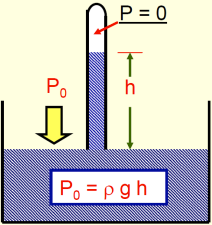
\includegraphics[width=5cm]{torricelli.png}
\end{center}
L’altezza del liquido nel tubo rovesciato dà una misura della pressione $P_0$ esercitata dal gas sulla superficie del contenitore più grande.\\
Si utilizza semplicemente la legge di Stevino: 
$$P_0=\rho g h$$
Occorre conoscere g e $\rho$: la prima varia con la 
latitudine mentre la seconda è funzione della 
temperatura.

%suca<3

\section{Tubo a U} 
Sono costituiti da un tubo (di solito trasparente) curvato ad U e riempito di un liquido di densità nota. Un'estremità del tubo è lasciata aperta all'atmosfera, mentre l'altra è in collegamento diretto con l'ambiente di misura. 
\begin{center}
    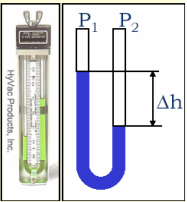
\includegraphics[width=5cm]{tubo_u.png}
\end{center}
Il liquido contenuto nel tubo si sposterà verso l'alto in uno dei due rami della U di un valore tale che la differenza di peso tra le due colonne di liquido bilanci esattamente la pressione (o depressione) presente nell'ambiente di misura. 
La differenza di pressione è data dal dislivello H tra i due menischi:
$$P_2-P_1=\rho g \Delta h$$
Il range di vuoto va dalla pressione atmosferica a qualche torr e la misura è indipendente dal tipo di gas. 
Un manometro di questo tipo ha l'inconveniente di essere fragile e non molto pratico.

\section{Vacuometro di Bourdon}
Il raggio di curvatura varia con la pressione interna al tubo $\rightarrow$ la misurazione del raggio dà la misura della pressione.\\
Questo vacuometro ha una robustezza meccanica e la misura è indipendente dal tipo di gas.\\
Un manometro di questo tipo ha l'inconveniente si avere una scarsa accuratezza al di sotto di $10$ mbar.
\begin{center}
    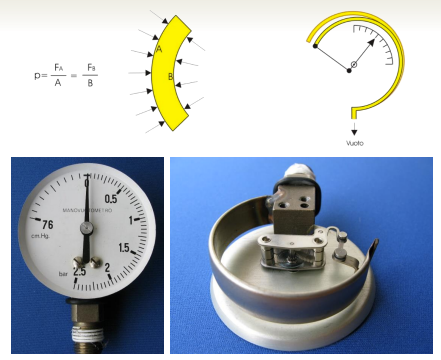
\includegraphics[width=8cm]{bourdon.png}
\end{center}

\section{Vacuometro di McLeod}
Misura assoluta della pressione P utilizzando un tubo ad U particolare, dove il volume di uno dei due bracci è molto maggiore dell’altro per via di un grosso bulbo di volume 
$V$.
\begin{center}
    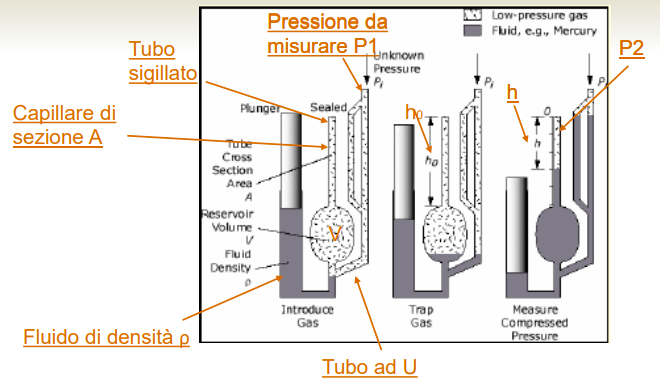
\includegraphics[width=8cm]{mcleod.png}
\end{center}
Il gas di cui si vuole misurare la pressione inizialmente occupa tutto il volume del tubo a U. Successivamente si spinge il liquido di misura, ad esempio mercurio, verso il tubo ad U (braccio sigillato).\\
Il liquido nel secondo braccio raggiunge un livello pari all’estremo superiore del capillare nel primo braccio del tubo ad U.\\
Il rapporto tra il volume del bulbo ed il volume del capillare sovrastante è molto grande ($\sim 10^5$). Questo rapporto $R$ costituisce una sorta di fattore di amplificazione della pressione da misurare $P_1$.
$$R=\frac{V}{Ah_0}$$
e il gas raggiunge la pressione $P_2\approx R\cdot P_1$
$$P_2=P_1+\rho g h\approx\rho g h ~~ (P_2>>P_1)$$
Attraverso alcune approssimazioni:
$$P_1\approx\frac{\rho g A}{V}h^2$$
\begin{itemize}
    \item Dalla misura della quota h si risale alla misura della pressione $P_1$;
    \item Scala quadratica molto vantaggiosa per la misura delle basse pressioni;
    \item Intervallo di misura $10^3$ Pa fino a $10^{-1}$ Pa, accuratezza $\sim 10\%$;
    \item Misura diretta della pressione assoluta del gas, non dipende dal tipo di gas stesso;
    \item Misura macchinosa, utilizzato come strumento per tarare i vacuometri a misura indiretta.
\end{itemize}

\section{Vacuometri Piezo-resistivi}
\begin{itemize}
    \item Piccolo volume pressurizzato a bassa pressione chiuso a tenuta da un diaframma;
    \item Il materiale piezo-resistivo depositato sul diaframma cambia la propria resistività in funzione dello sforzo meccanico applicato;
    \item Dalla misura della resistenza si risale alla pressione applicata al diaframma;
    \item Intervallo di misura da 1 mbar fino a circa 2000 mbar;
    \item Vantaggi: lettura digitale, robustezza, costo contenuto, velocità;
    \item Svantaggi: necessaria calibrazione frequente;
\end{itemize}
\begin{center}
    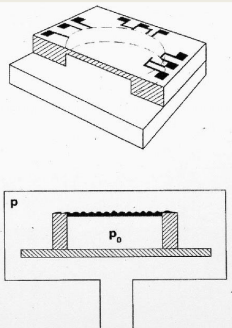
\includegraphics[width=5cm]{piezo_resistivi.png}
\end{center}

\section{Vacuometro Pirani}
Nel caso del vacuometro Pirani il filamento viene inserito in un ponte di Wheatstone.
\begin{center}
    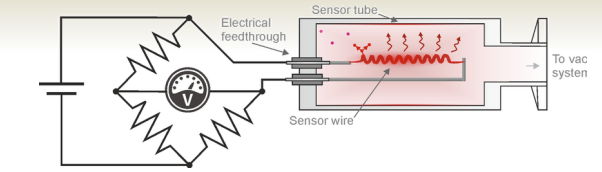
\includegraphics[width=12cm]{pirani.png}
\end{center}
La temperatura di $R_2$ è il risultato dell'equilibrio termico che si viene a creare tra calore dissipato dal filamento per effetto Joule ($P=I^2R$) e il calore ceduto al gas per conduzione.\\
La variazione di pressione comporta una variazione di calore trasmessa al gas e di conseguenza una variazione di temperatura del filamento e quindi di $R_2$. La variazione di $R_2$ provoca lo sbilanciamento del ponte con indicazione di corrente da parte del galvanometro.\\
Vantaggi:
\begin{itemize}
    \item Semplicità costruttiva;
    \item Robustezza meccanica.
\end{itemize}
Limiti:
\begin{itemize}
    \item Valore di pressione dipendente dal tipo di gas;
    \item Variazione dello zero a causa di contaminazione del filamento.
\end{itemize}


\section{Vacuometro a termocoppia}
\begin{itemize}
    \item Una variazione di pressione determina una variazione di temperatura di un filamento riscaldato.
    \item La temperatura è misurata mediante una termocoppia fissata al filamento riscaldatore che a sua volta è riscaldato da un generatore di corrente costante.
    \item L'uscita della termocoppia è letta su di un amperometro calibrato direttamente in unità di pressione.
\end{itemize}


\begin{center}
    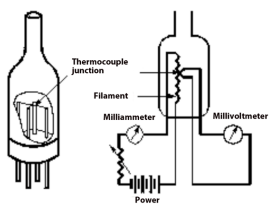
\includegraphics[width=8cm]{termocoppia.png}
    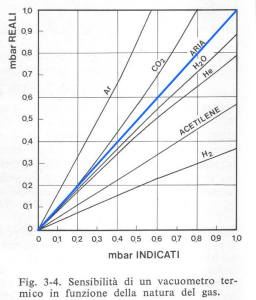
\includegraphics[width=5cm]{pirani2.png}
\end{center}


\newpage
\section{Vacuometro Penning}
Il vacuometro più diffuso per misure di pressione nell'intervallo di $10^{-3}-10^{-6}$ Pa è senza dubbio il \textit{vacuometro Penning}, detto anche vacuometro a catodo freddo.
\begin{center}
    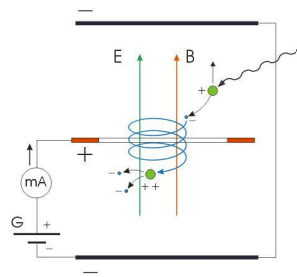
\includegraphics[width=8cm]{penning.png}
\end{center}
Nell'ampolla sono sistemati due elettrodi (catodo e anodo) di materiale a basso potenziale di estrazione che vengono alimentati con una differenza di potenziale di alcune migliaia di volt. Il catodo è costituito da due piastre connesse elettricamente, mentre l'anodo è costituito da un piccolo telaio opportunamente sagomato. L'ampolla è collegata al recipiente sotto vuoto.\\
Se il vuoto è tale che il libero cammino medio delle molecole del gas è uguale all'incirca alle dimensioni lineari dell'ampolla, gli ioni presenti in esso migrano verso gli elettrodi ed ivi strappano degli elettroni, che, accelerati dal campo, possono produrre altri ioni e quindi determinare una corrente circa proporzionale al numero delle molecole presenti nel vacuometro.\\
Tale corrente è misurata mediante un microamperometro inserito nel circuito. Per aumentare l'intensità di corrente in modo che la misura possa essere eseguita più facilmente e con più elevata sensibilità, si utilizza un magnete permanente che produce un campo di alcune centinaia di Oersted.\\
In virtù della particolare configurazione degli elettrodi e della disposizione del magnete, il campo elettrico ha in ogni punto una componente ortogonale del magnete. In pratica le linee di forza del campo elettrico e di quello magnetico si intersecano e quindi le orse di natura elettrica e magnetica applicate agli elettroni determinano la traiettoria a forma di spirale degli elettroni. Il percorso che essi compiono, aumenta di un centinaio di volte rispetto a ciò che avrebbe in assenza di campo magnetico. Aumenta così la probabilità di collisione tra gli elettroni e le molecole del gas ed è prodotto un numero maggiore di ioni a parità di pressione. Il grande vantaggio dei vacuometri Penning è l'eccezionale semplicità e robustezza costruttiva. Gli svantaggi sono la dipendenza dal tipo di gas e il raggiungimento di un limite inferiore e superiore rispettivamente di $10^{-4}$ e $10^{-1}$ Pascal.



\chapter{Elettronica}
\section{Segnali dai rivelatori ed elettronica associata}
I primi rilevatori di particelle erano \textit{rivelatori visuali} cioè basati sulla visualizzazione delle tracce impresse su pellicole, lasciate dalle particelle al loro passaggio interagendo con la materia. Dalle caratteristiche della traccia era possibile stimare l'energia della particella (in base alla lunghezza della traccia) e la sua entità, in quanto le particelle pesanti lasciavano una traccia più marcata.
Ad esempio nella figura sottostante vi è la traccia lasciata da un nucleo di Uranio in una emulsione nucleare.
\begin{center}
    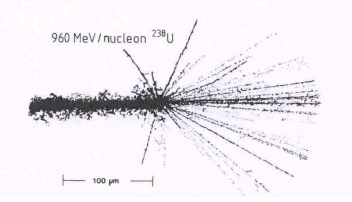
\includegraphics[width=8cm]{ele1.png}
\end{center}
Veniva fatto largo uso di strumenti di rilevazione quali le camere a bolle e le camere a nebbia.
La \textit{camera a bolle} è costituita da un recipiente metallico cilindrico contenente un liquido in
condizione metastabile.\\
Una particella carica veloce che attraversi il recipiente ionizza molti atomi del liquido, perdendo nel contempo parte della sua energia pur senza subire deviazioni apprezzabili. Lungo il percorso della particella vengono a trovarsi ioni positivi e negativi attorno a cui il liquido inizia a bollire e le bollicine che si creano possono ingrandirsi fino a riempire tutta la camera. Scattando diverse foto da angolazioni differenti, si ottiene una ricostruzione stereoscopica spaziale delle tracce.\\
Per poter riutilizzare nuovamente la camera a bolle è necessario aumentare la pressione per far cessare l’ebollizione del liquido, per poi ripristinare la situazione metastabile. Solitamente una camera a bolle è circondata da un grosso magnete il cui campo magnetico, omogeneo in tutto lo spazio della camera, deflette le particelle cariche lungo una traiettoria circolare (ossia realizza un ciclotrone) il cui raggio dipende dalla quantità di moto delle particelle. Analizzando le tracce, si hanno informazioni sulla massa e sulla velocità delle particelle. Dal raggio di curvatura si ricava l’impulso della particella.
\begin{center}
    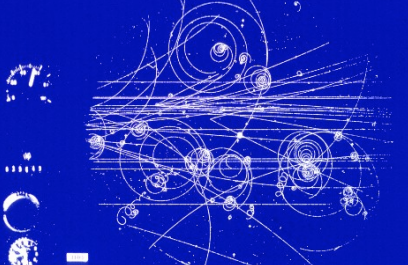
\includegraphics[width=8cm]{bolle.png}
    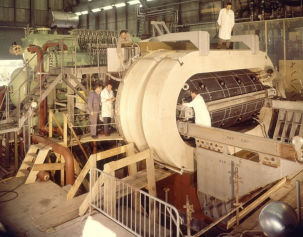
\includegraphics[width=8cm]{bolle1.png}
\end{center}
La \textit{camera a nebbia} consiste in una scatola a tenuta ermetica che contiene aria satura di vapore acqueo collegata, mediante un condotto, ad un cilindro entro il quale scorre un pistone. Un rapido spostamento dello stantuffo provoca nella camera un'espansione adiabatica del vapore che passa allo stato instabile di sovrasaturazione. In tali condizioni una qualsiasi particella elementare carica elettricamente che penetri nella scatola ionizzando gli atomi con i quali si scontra crea, lungo il proprio tragitto, un fitto susseguirsi di nuclei di condensazione (atomi ionizzati), attorno ai quali il vapore sovrasaturo si raccoglie a formare minuscole goccioline (nebbia). La traccia lasciata dalla traiettoria percorsa della particella può essere fotografata attraverso una parete trasparente della scatola e da questa si può risalire, con particolari accorgimenti, alla determinazione della natura della particella. Prima di ripetere il ciclo è opportuno rimuovere gli ioni attraverso un campo elettrico e rieffettuare la compressione.\\
Nelle camere a nebbia moderne lo scatto del pistone è comandato, con l'ausilio di un circuito elettronico, dall'arrivo stesso della particella da studiare.
\begin{center}
    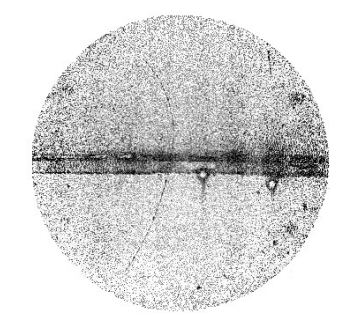
\includegraphics[width=8cm]{nebbia.png}
\end{center}
L'analisi queste tracce richiedeva in genere un lungo lavoro manuale. Successivamente, fu possibile eseguire l'analisi dei dati, che prima veniva effettuata manualmente, in modo digitale sviluppando dei fotogrammi della traccia e facendoli analizzare da un computer.\\
I rilevatori più recenti producono un segnale elettrico di varia natura, che fornisce informazioni sul tipo di particella, sull'energia, sul tempo di arrivo...
\begin{center}
    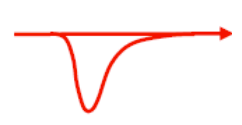
\includegraphics[width=8cm]{ele2.png}
\end{center}
Essi necessitano, però, di una opportuna elettronica.\\
Maggiore è il numero di cavi connessi ad un rilevatore e maggiore è il numero di informazioni (segnali) ottenibile. Ad esempio un contatore Geiger presenta un solo cavo perchè l'unica informazione che fornisce è il passaggio di una particella. Ovviamente i cavi servono anche per
l'alimentazione dei rilevatori e per i segnali di controllo delle apparecchiature.\\
I cavi trasportano alte e basse tensioni e segnali di varia natura proveniente dai rilevatori e dai circuiti di controllo.\\
Per estrarre l'informazione dai rivelatori è necessario che il segnale sia processato da un sistema elettronico, allo scopo di:
\begin{itemize}
    \item Distinguere segnali di tipo differente;
    \item Estrarre l'informazione sull'energia;
    \item Estrarre l'informazione temporale.
\end{itemize}
In fisica nucleare l’informazione è tipicamente sotto forma di segnali impulsivi, in corrente o tensione, e l’informazione è legata ad una o più caratteristiche del segnale, ad esempio l’ampiezza, la polarità, la forma del segnale, il tempo al quale si osserva 
un dato segnale,..
Andiamo a definire alcune terminologie utili:
\begin{itemize}
    \item \textit{Baseline}: livello al quale il segnale tende asintoticamente (è una sorta di rumore di fondo costante o variabile);
    \item  \textit{Ampiezza (o pulse height)}: è la distanza tra la baseline e il picco del segnale;
    \item \textit{FWHM}: larghezza a metà altezza;
    \item \textit{Leading edge}: il fronte iniziale del segnale;
    \item \textit{Falling (trailing) edge}: fronte finale del segnale;
    \item \textit{Rise time}: tempo che il segnale impiega per passare dal $10\%$ al $90\%$ della sua ampiezza (tempo di salita);
    \item \textit{Fall time}: tempo che il segnale impiega per decadere dal $90\%$ al $10\%$ della sua ampiezza (tempo di discesa).
\end{itemize}
\begin{center}
    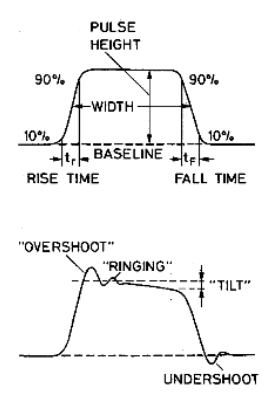
\includegraphics[width=8cm]{ele3.png}
\end{center}
I segnali possono distinguersi in:
\begin{itemize}
    \item \textit{Unipolari}: il segnale crea un solo lobo;
    \item \textit{Bipolari}: il segnale segnale attraversa la base line creando due lobi;
    \begin{center}
        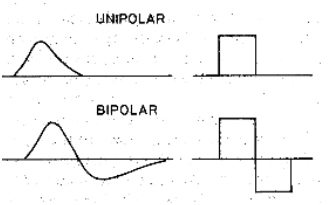
\includegraphics[width=8cm]{ele4.png}
    \end{center}
    \item \textit{Analogici}: l’informazione è codificata in modo continuo in una caratteristica del segnale (ampiezza, forma), proporzionale al valore dell’informazione (ad esempio l’energia);
    \item \textit{Logici}: i segnali hanno solo un numero discreto di stati (tipicamente 0 e 1), codificati in qualche modo. Anche se trasportano meno informazione rispetto ad un segnale analogico, sono più affidabili in quanto è più difficile che l’informazione sia deteriorata;
    \item \textit{Veloci}: tempi di salita di alcuni nano secondi o meno, vengono utilizzati nell'applicazione di timing ed alte frequenze di conteggio, possono essere distorti da piccole componenti capacitive, induttive e resistive presenti nei circuiti e nelle loro interconnessioni;
    \item \textit{Lenti}: tempo di salita di circa 100 nanosecondi o più, vengono utilizzati in spettroscopia essendo più immuni al rumore.
\end{itemize}
In figura sono riportati rispettivamente un esempio di segnale veloce e di segnale lento:
\begin{center}
    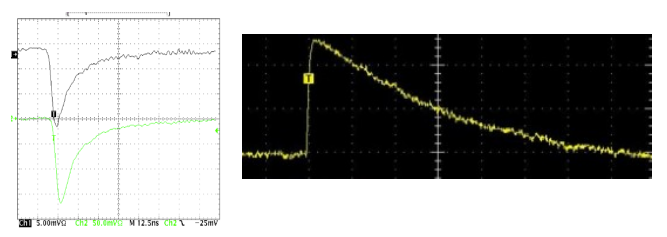
\includegraphics[width=14cm]{ele5.png}
\end{center}
In elettronica ci si riferisce comunemente alla \textit{banda passante} come l'intervallo di frequenze che un dato segnale contiene o che un dato apparecchio è in grado di trattare. Più specificatamente, data la risposta in frequenze di un dato dispositivo o segnale, l'ampiezza della sua banda passante è uguale alla differenza tra le due frequenze massima e minima (cioè quelle che normalmente vengono
attenuate di $3dB$ rispetto ad una frequenza cosiddetta centrale) che esso lascia passare.
$1dB=10\log\frac{V_1}{V_2}$
quindi $3$ decibel equivale a dire:
$10\log\frac{\nu_1}{\nu_2}=3 \implies \log\frac{\nu_1}{\nu_2}=0.3$
$$\implies \frac{\nu_1}{\nu_2}=10^{0.3}=1.995$$
\begin{center}
    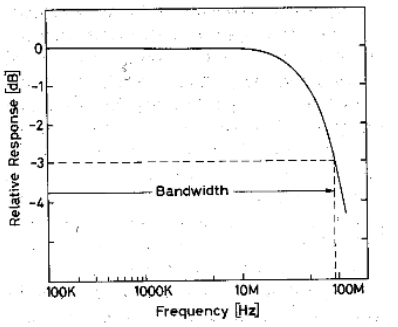
\includegraphics[width=8cm]{ele6.png}
\end{center}
In elettronica nucleare riveste una certa importanza considerare i segnali in termini di componenti spettrali.\\
\'E noto che mediante la trasformata di Fourier ogni segnale $f(t)$ può essere decomposto in una sovrapposizione di segnali sinusoidali puri:
$$f(t)=\frac{1}{\sqrt{2\pi}\int_{-\infty}^{+\infty}g(\omega)\exp(i\omega t)d\omega}$$ 
dove $g(\omega)$ è la \textit{trasformata di Fourier} di $f(t)$.\\
Invertendo si ha $$g(\omega=\frac{1}{\sqrt{2\pi}\int_{-\infty}^{+\infty}f(t)\exp(-i\omega t)dt}$$
Data una trasformata di Fourier $g(\omega)$ di un impulso rettangolare $f(t)$
\begin{center}
    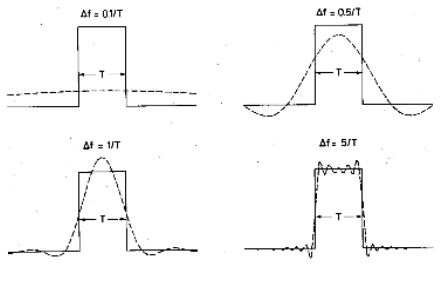
\includegraphics[width=8cm]{ele7.png}
\end{center}
La trasformazione inversa limita il range di integrazione fino ad una certa frequenza di taglio $\Delta f$.\\
Una minima banda passante $\Delta f \geq \frac{1}{T}$ è necessaria per fornire una ragionevole approssimazione dell'impulso. In conclusione, quindi, scelto una opportuna banda passante $\Delta f$ è possibile riportare il segnale ad uno sviluppo in serie di Fourier.\\
La tipica elettronica nucleare ha bande passanti dell'ordine di $500 Mhz$. Ad esempio per trattare impulsi da $5$ nanosecondi vi sono bande passanti almeno dell'ordine $200 Mhz$.\\
Per passare da un segnale analogico ad un segnale digitale è necessario assegnare alla baseline il valore 0 e al picco il valore 1. Si utilizza, pertanto, un discriminatore avente soglia regolabile tale da far passare segnali a partire da un certa ampiezza. L'onda in ingresso viene trasformata in un'onda quadra.
\begin{center}
    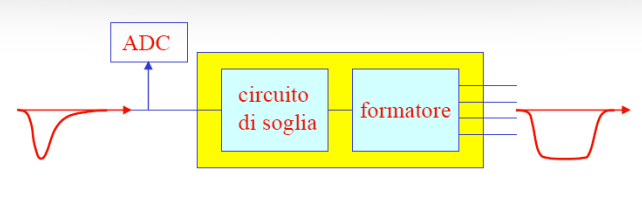
\includegraphics[width=8cm]{ele8.png}
    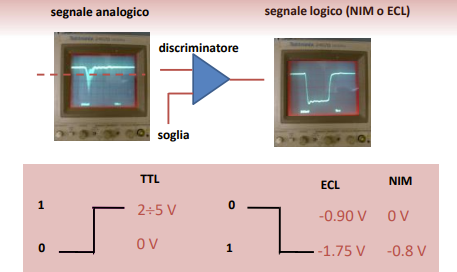
\includegraphics[width=8cm]{ele9.png}
\end{center}
I segnali standard digitali (o logici) consistono in valori iniziali e finali di tensioni associati a transizioni di onde quadre positive o negative. \\
I segnali analogici a differenza di quelli logici sono  soggetti a distorsioni dovute al rumore di fondo, per tale ragione spesso si preferisce lavorare con i secondi anziché con i primi.\\
Alcuni tra i i più importatnti segnali logici sono:
\begin{itemize}
    \item \textit{TTL}:\\ 
    "TTL" significa letteralmente "Transistor-Transistor Logic". \'E il sistema basato sul combinare i transistori in modo tale che essi possano venire usati come delle porte logiche (logica positiva talvolta utilizzata in moduli di elettronica NIM). I transistori hanno la capacità di diventare parte di dispositivi molto complessi quando siano combinati.
    \item \textit{ECL}:\\ 
    “ECL” significa letteralmente “Emitter Coupled Logic”. \'E un sistema basato sulla combinazione di transistor secondo configurazioni differenziali. Questa è una logica più moderna ed è molto veloce nonostante necessiti di una conversione per essere utilizzata in standard NIM e CAMAC.
\end{itemize}
La \textit{trasmissione di un segnale} è un concetto apparentemente banale che consiste nel trasferimento di un'informazione, analogica o digitale, da un punto ad un altro di un sistema, senza deteriorare la qualità dell'informazione stessa.\\
Da un punto di vista meramente concettuale un segnale contiene un intervallo di frequenze illimitato ma in realtà si fissa, generalmente, un limite superiore di $1GHz$.\\
Per trasportare il segnale si utilizzano dei \textit{cavi coassiali}. Nella parte più interna vi è un cavo conduttore che trasporta il segnale, questo è poi rivestito da una guaina dielettrica di separazione tra segnale e massa, a sua volta contenuta in uno schermo di fili intrecciati (ritorno a terra, filtri da campi elettromagnetici) ed infine vi è un ultima guaina di rivestimento.
\begin{center}
    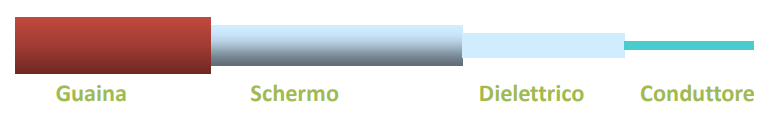
\includegraphics[width=8cm]{coassiale.png}
\end{center}
La presenza del dielettrico induce un ritardo nel trasporto del segnale all'interno del cavo dell'ordine di 5 nanosecondi (per i cavi utilizzati usualmente in laboratorio).\\ 
Sul mercato vi è una larga varietà di cavi caratterizzati da diversi valori di impedenza, capacità e ritardo. I più utilizzati sono l'\textit{RG-58C/U} e il \textit{RG-174/U} (50 Ohm).
\begin{center}
    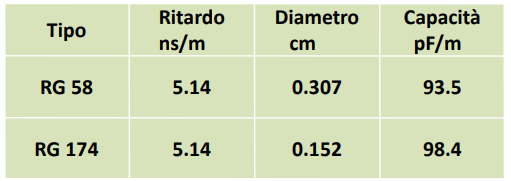
\includegraphics[width=8cm]{coassiale2.png}
\end{center}
L'impedenza caratteristica assume notevole importanza per le riflessioni del segnale lungo la linea coassiale. Si deve tener conto dell'impedenza $Z0$ del cavo perchè se questo viene collegato ad un circuito la cui impedenza è $Z\neq Z_0$ una parte del segnale verrà riflessa.\\ 
Supponiamo di trasmettere un segnale lungo un cavo coassiale di impedenza $Z_0$ lungo la linea $V =Z_0I$ . Quando il segnale raggiungerà un carico di impedenza diverso, la legge di Ohm dovrà tener conto anche del carico e del segnale che deve propagarsi in direzione opposta al cavo, cioè:
$$\frac{V}{I}=Z_0 ~~ \frac{V_r}{-I_r}=Z_0 \implies \frac{V+V_r}{I+I_r}=R$$
definendo con $\rho$ la quantità $\frac{V_r}{V}$, si trova che il \textit{coefficiente di riflessione} del segnale in un cavo è
$$\rho=\frac{Z-Z_0}{Z+Z_0}$$
Possiamo distinguere tre casi "limite":
\begin{itemize}
    \item $R=0 \implies \rho=-1$: il segnale originale viene riflesso completamente ma invertito di polarità (corto circuito);
    \item $R=Z_0\implies \rho=0$: il segnale non subisce distorsioni o alterazioni di alcun tipo e prosegue indisturbato il suo cammino;
    \item $R=\infty \implies \rho=1$: il segnale originale viene riflesso completamente.
\end{itemize}
\'E necessario “terminare” un cavo coassiale con la sua resistenza caratteristica per evitare distorsioni nel segnale.\\ 
Lo standard NIM parzialmente risolve questo problema poiché la larga maggioranza dei moduli viene prodotta con impedenze in ingresso ed uscita pari a 50 Ohm.\\
In alcuni casi, come ad esempio negli oscilloscopi, ciò non è possibile e pertanto la terminazione può essere realizzata mediante resistenze esterne.\\
Nella figura che segue è riportato un esempio di una distorsione di un impulso rettangolare dovuta ad un disadattamento di impedenza:
\begin{center}
    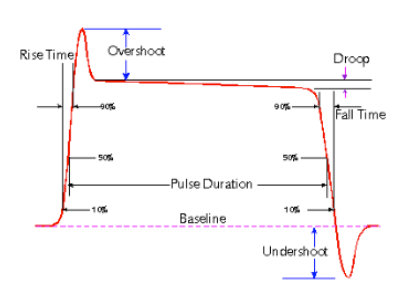
\includegraphics[width=8cm]{distorsione.png}
\end{center}
Per scegliere al meglio il cavo da utilizzare è utile valutare la relazione tra lunghezza-attenuazione-frequenza tramite l'utilizzo di \textit{nomogrammi} oppure, in alternativa, utilizzare specifici siti Web on-line.\\
Un importante fattore di cui è necessario tener conto è l'\textit{attenuazione del segnale} che si misura in $decibel /100m$ e dipende dalla frequenza del segnale stesso, in quanto maggiore è la frequenza e maggiore sarà l'attenuazione.\\ 
Quest'ultima si calcola mediante l'espressione:
$$RL=\frac{R*L}{100}$$
$$ALL=RL\sqrt{\frac{FA}{FR}}$$
dove:
\begin{itemize}
    \item R: valore conosciuto della perdita ad una data frequenza ($dB/100 m$ o $dB/100 ft$);
    \item L: lunghezza del cavo (m o ft);
    \item FR: frequenza alla quale è data la perdita (MHz);
    \item FA: frequenza di lavoro alla quale si vuole calcolare la perdita (MHz);
    \item ALL: perdita totale del cavo a lunghezza L e frequenza FA.
\end{itemize}

\section{Connettore BNC}
Un \textit{connettore elettrico} è un componente elettrico che la funzione di collegare elettricamente due o più componenti esclusivamente mediante operazioni di tipo meccanico (quindi senza necessità di saldature). Esistono molti tipi di connettori elettrici che soddisfano esigenze diverse: maschio, femmina, T, I, adatatori...\\
I \textit{connettori BNC} sono una famiglia di connettori unipolari a baionetta usati per l'intestazione di cavi coassiali. L'aggancio fra il connettore maschio e il connettore femmina si effettua ruotando di un quarto di grado la ghiera del connettore maschio intorno ai due perni ricavati sulla ghiera del connettore femmina, l'unione così ottenuta risulta meccanicamente molto affidabile. Gli elementi del contatto possono essere placcati in argento, oro o teflon. Quest'ultimo è un eccezionale elemento isolante.\\
I connettori BNC vengono utilizzati per cablare segnali di
vario tipo.
\begin{center}
    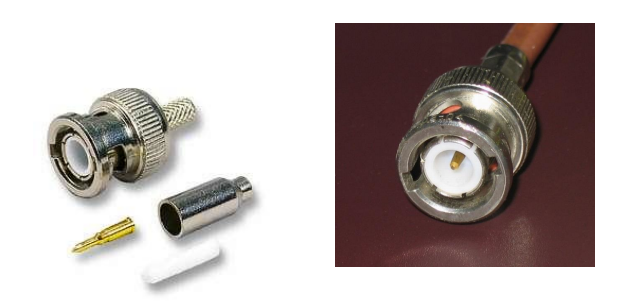
\includegraphics[width=8cm]{BNC.png}
\end{center}

\section{Gli oscilloscopi}
L'oscilloscopio è uno strumento di misura elettronico che consente di visualizzare, su un grafico bidimensionale, l'andamento temporale dei segnali elettrici e di misurare abbastanza semplicemente tensioni, correnti, potenze ed energie elettriche.\\
L'asse orizzontale del grafico solitamente rappresenta il tempo, rendendo l'oscilloscopio adatto a misurare grandezze periodiche. L'asse verticale rappresenta la tensione. La frequenza massima dei segnali visualizzabili, così come la risoluzione temporale, ovvero la più rapida variazione rilevabile, dipende dalla banda passante dello strumento.\\
\'E di fondamentale importanza la \textit{banda passante} dell'amplificatore di ingresso per fare in modo che l’oscilloscopio rappresenti il segnale in modo corretto, in particolare per quel che riguarda il tempo di salita dei segnali, una sua formula approssimata è la seguente:
$$t_{osc}=\frac{350}{f_{3dB}[MHz]}$$
Se ho un segnale con un fronte di salita $t_{rise}$, questo verrà visto sull’oscilloscopio con un tempo di salita $t_{meas}$ pari a:
$$t_{meas}=\sqrt{t_{rise}^2+t_{osc}^2}$$
il segnale è leggermente deformato, perchè il tempo è leggermente maggiore a causa della banda passante.\\
Come ogni buon voltmetro, l'oscilloscopio ha un'alta impedenza di ingresso, tipicamente di $1M\Omega$, in parallelo con una capacità di qualche decina di $pF$. \'E possibile cambiare l'impedenza all'ingresso a $50\Omega$ direttamente sull'oscilloscopio, per terminare correttamente il cavo che trasporta il segnale.\\
Lo stadio d'ingresso può essere:
\begin{itemize}
    \item DC: accoppiata in continua (modalità normale di funzionamento);
    \item AC: viene filtrata la componente in continua;
    \item GND l'ingresso è messo a ground (messa a terra).
\end{itemize}
Un oscilloscopio ha tipicamente tra 2 e 4 ingressi indipendenti.\\
L'oscilloscopio può essere considerato uno strumento universale in quanto collegandovi appropriati trasduttori si può analizzare qualsiasi fenomeno fisico.\\
Il segnale da misurare viene introdotto attraverso un apposito connettore, solitamente di tipo coassiale BNC adatto per frequenze relativamente basse. Al connettore di ingresso possono essere collegate le sonde, accessori particolari usati per prelevare segnali dai circuiti che devono essere analizzati.\\
La velocità di scansione è selezionabile per mezzo di una manopola presente sul pannello, la quale comanda il circuito chiamato base dei tempi, questo circuito genera precisi  intervalli di tempo, che possono spaziare da pochi secondi a qualche nanosecondo.\\
In assenza di segnale  la traccia è solitamente al centro dello schermo, l'applicazione di un segnale
all'ingresso provoca la deflessione verso l'alto o verso il basso, in funzione della polarità del segnale. La scala verticale è solitamente espressa in multipli di volt e l'altezza iniziale del grafico, ovvero l'offset, può essere decisa dall'utente, così come è possibile escludere la corrente continua presente nel segnale in esame, nonché scegliere l'impedenza di ingresso.\\
In questo modo si ottiene la visualizzazione di un grafico di tensione in funzione del tempo. Se il segnale è periodico, è possibile ottenere una traccia stabile regolando la base dei tempi in modo da farla coincidere con la frequenza del segnale o con un suo sottomultiplo, tale processo è chiamato
sweep continuo.\\
Per ottenere una traccia stabile gli oscilloscopi moderni dispongono di una funzione chiamata \textit{trigger} (innesco). Il trigger è un circuito elettronico che sincronizza la partenza della scansione orizzontale con un preciso livello di soglia del segnale periodico da analizzare. Dopo aver completato la scansione da sinistra a destra, l'oscilloscopio rimane in attesa di un nuovo evento. In questo modo la visualizzazione rimane sincronizzata al segnale e la traccia è perfettamente stabile. \\
Il circuito del trigger può essere configurato per mostrare una sola scansione di un segnale non periodico, come un singolo impulso o sequenze impulsi non ripetitivi. È possibile introdurre un ritardo tra l'evento e l'inizio della visualizzazione, in modo da analizzare parti del segnale che altrimenti sarebbero fuori dal campo di visualizzazione.
\begin{itemize}
    \item Sorgente del trigger:
    \begin{itemize}
        \item Internal: il riferimento usato è uno dei segnali;
        \item External: un canale aggiuntivo usato solo per un segnale di trigger;
    \end{itemize}
    \item Condizioni:
    \begin{itemize}
        \item Slope: trigger su fronte discesa o salita;
        \item Level: valore della soglia alla quale scatta il trigger;
    \end{itemize}
    \item Modi:
    \begin{itemize}
        \item Normal: trigger solo se sono verificate le condizioni;
        \item Auto: autotrigger (analog) o anche autolevel;
        \item Single: un solo campionamento o una sola sweep alla volta.
    \end{itemize}
\end{itemize}

\newpage
\section{Differenze tra oscilloscopi analogici e digitali}

\begin{center}
\resizebox{\linewidth}{!}{%
\begin{tabular}{l|l|l|ll}
\cline{2-3}
 & ANALOGICO & DIGITALE &  &  \\ \cline{1-3}
\multicolumn{1}{|l|}{Accuratezza} & Dipende dalla BW del sistema. & \begin{tabular}[c]{@{}l@{}}Dipende dalla BW analogica \\ e dalla frequenza \\ di campionamento.\end{tabular} &  &  \\ \cline{1-3}
\multicolumn{1}{|l|}{Ripetition rate} & \begin{tabular}[c]{@{}l@{}}Idealmente 1/sweep\_time; \\ l’intensità è proporzionale \\ alla freq. di trigger; grazie \\ alla "memoria" del fosforo molte \\ forme d'onda possono essere \\ visualizzate assieme!\end{tabular} & \begin{tabular}[c]{@{}l@{}}Dipende; nei primi modelli \\ poche forme d'onda/s; nei nuovi \\ (DPO, digital phosphor) anche \\ 3600/s,e simulazione \\ digitale della memoria dei \\ fosferi.\end{tabular} &  &  \\ \cline{1-3}
\multicolumn{1}{|l|}{Singoli eventi} & Praticamente invisibili o quasi. & \begin{tabular}[c]{@{}l@{}}Se ci sono si vedono (se si \\ riescono a triggerare), ma \\ se sono rari occorrono alte \\ frequenze di acquisizione \\ (5 GS/s nel TD3054B).\end{tabular} &  &  \\ \cline{1-3}
\multicolumn{1}{|l|}{Trigger} & Tradizionalmente solo un livello. & \begin{tabular}[c]{@{}l@{}}trigger avanzato su livelli, \\ combinazioni logiche \\ di segnali,...\end{tabular} &  &  \\ \cline{1-3}
\multicolumn{1}{|l|}{Altro} & Poco altro. & \begin{tabular}[c]{@{}l@{}}Storage dei segnali, analisi \\ dei segnali in tempo \\ reale, ...\end{tabular} &  &  \\ \cline{1-3}
\end{tabular}%
}
\end{center}





\newpage
\section{Modulistica elettronica}
Lo standard NIM, ovvero Nuclear Instrument Module, vene stabilito nel 1964 ed è il primo vero e proprio standard introdotto in fisica delle alte energie.  ad esso sono state fissate le dimensioni meccaniche dei crate, l'alimentazione, il numero di stazioni per ogni crate, gli amplificatori, i discriminatori, moduli di ritardo.\\
I principali moduli in elettronica sono:
\section{Linee di ritardo}
Sono semplici moduli (attivi o passivi) utilizzati per introdurre un ritardo tra un segnale in ingresso e uno in uscita.\\
Introducono attenuazione del segnale.
Per “piccoli” ritardi ($\sim100 ns$) si sfrutta la velocità di propagazione nei cavi coassiali ($5 ns/m$). 
Per ritardi maggiori (micro o milli secondi) non possono essere ottenuti in questo modo, e necessitano elettronica attiva.

\section{Fan-in}
Moduli attivi in cui l'uscita è la somma analogica dei segnali in ingresso. Possono essere sia lineari che logici. In quest'ultimo caso la somma è l'OR dei segnali in ingresso. Possono accettare in ingresso segnali di una data polarità o bipolari.\\
Possono essere sia lineari che logici.
\begin{center}
    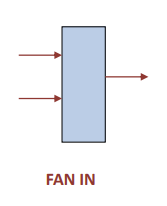
\includegraphics[width=3cm]{fanin.png}
\end{center}
\section{Fan-out}
moduli attivi in cui un singolo segnale viene distribuito su varie uscite. Da non confondersi con gli “splitters” passivi.\\
Possono essere sia lineari che logici.
\begin{center}
    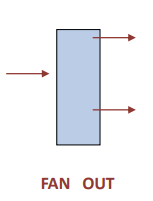
\includegraphics[width=3cm]{fanout.png}
\end{center}
\section{Discriminatori}
I discriminatori generalmente vengono utilizzati nei sistemi di trigger e per la misura dei tempi o dei conteggi.\\
Producono un segnale logico standard in uscita se e solo se il segnale analogico in ingresso è superiore ad un certo valore di soglia.\\ 
Il segnale in uscita è un segnale logico standard NIM la cui larghezza è modificabile mediante un potenziometro. La soglia elimina i possibili rumori di fondo e qualsiasi informazione sull'ampiezza dell'impulso iniziale si perde.
Le soglie variano da $20$ a $1000 mV$ mentre le larghezze da $5$ a $1000 ns$.
\begin{center}
    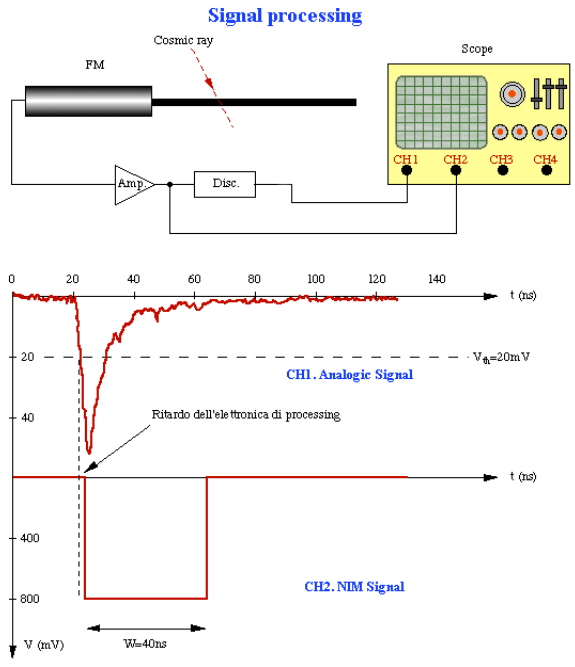
\includegraphics[width=8cm]{discriminatore.png}
\end{center}
Vi sono due tipi di discriminatori:
\begin{itemize}
    \item \textit{Discriminatori “leading edge”}:\\
    segnali di ampiezza diversa (ma stessa forma!) hanno un segnale in uscita diverso\\ 
    $\implies$ indeterminazione nella misura temporale, necessità di una correzione dipendente dall’ampiezza del segnale (che deve essere quindi necessariamente misurata...);
    \begin{center}
         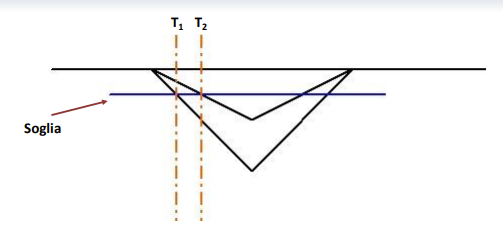
\includegraphics[width=8cm]{discriminatore2.png}
    \end{center}
    \item \textit{Discriminatori “a frazione costante” (CFD)}:\\
    il discriminatore non “scatta” ad una data soglia (in mV) ma ad una determinata frazione dell’ampiezza del segnale: misura del tempo praticamente indipendente dall’ampiezza dell’impulso.
    \begin{center}
        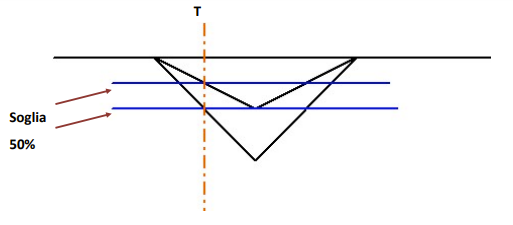
\includegraphics[width=8cm]{discriminatore3.png}
    \end{center}
    Di seguito lo schema di funzionamento di un CFD.
    \begin{center}
        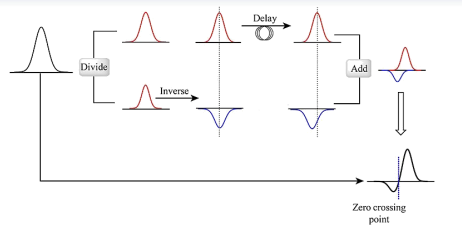
\includegraphics[width=12cm]{cdf.png}
    \end{center}
\end{itemize}

\section{Scale di conteggio (Scaler)}
Sono semplici contatori di impulsi digitali. Moduli NIM, CAMAC o VME. Sono programmabili e dotati di un display a LED oppure soltanto “leggibili” mediante computer. Possono lavorare a frequenze di conteggio continuo fino a 100MHz. Sono segnali di CLEAR e INHIBIT.

\section{Coincidenze (AND)}
Le coincidenze appartengono ad un'ampia classe di moduli di unità logiche e vengono utilizzate spesso, nei sistemi di Trigger veloci, dove è necessario imporre la coincidenza di uno o più rilevatori.\\
Le unità di coincidenza sono delle unità che danno un segnale quando tutti e due gli ingressi di due rilevatori forniscono contemporaneamente un segnale, cioè quando il segnale è contemporaneamente uno per entrambi. Se quest'ultimo è lento allora l'unità di coincidenza può essere costruita semplicemente mediante un circuito integrato mentre se il segnale è veloce il circuito risulta essere particolarmente complesso in quanto vi sono degli standard NIM che consistono in moduli AND a più ingressi (massimo 4). 
\begin{center}
    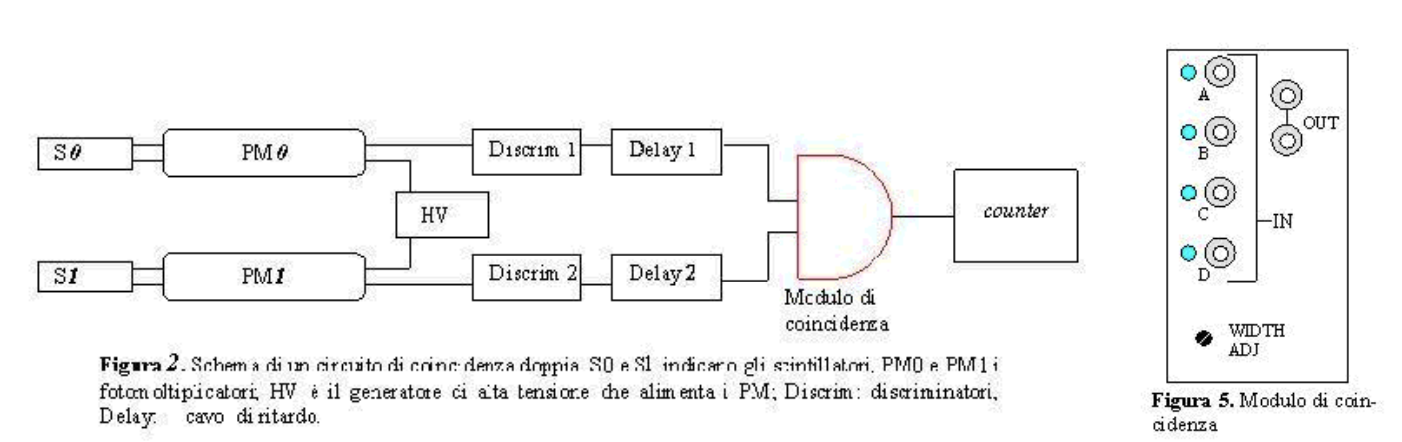
\includegraphics[width=14cm]{coincidenze1.png}
\end{center}
Si osservi che la coincidenza si ha quando vi è anche una sola sovrapposizione parziale del segnale e pertanto si può stabilire un'ampiezza di tempo entro la quale due segnali possono essere considerati coincidenti.\\
Ovviamente si deve fare in modo che la finestra temporale utilizzata per stabilire la coincidenza sia la più piccola possibile.
\begin{center}
    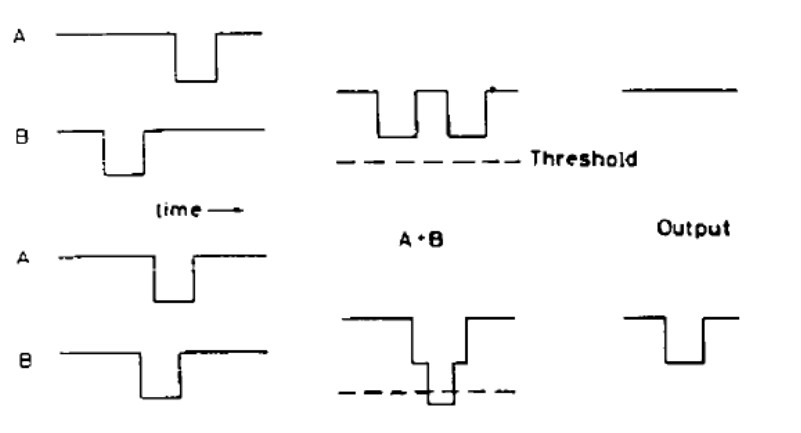
\includegraphics[width=8cm]{coincidenze2.png}
\end{center}
Sia $\Delta T$ la lunghezza dei segnali discriminanti (finestra temporale), $S_0$ la frequenza di conteggio singolo di $S_0$ ed $S_1$ la frequenza di $S_1$ allora la “\textit{frequenza di conteggi spuri}” sarà:
$$R_{acc}\simeq 2S_0S_1\Delta T$$
dove una coincidenza spuria è la coincidenza di due segnali che non sono realmente coincidenti.\\ 
Non si riescono a distinguere con quelle effettive, fare una stima di esse è utile per sottrarle dal risultato finale. Se si avessero più di due sorgenti, ad esempio $n$, la formula generale è
$$R_{acc}\simeq 2S_1...S_n\Delta T^{n-1}$$

\section{Unità logiche}
Generalmente sono moduli NIM e le unità logiche sono di varia natura (AND, OR, NOT).\\
Moduli di tipo CAMAC o VME più frequentemente utilizzati in fisica delle particelle. Multi-ingresso (fino a 32 ingressi contemporanei), logiche programmabili, normalmente utilizzano lo standard ECL.

\section{Moduli di alimentazione}
Oltre agli alimentatori tradizionali singoli, esistono anche moduli di alimentazione standard NIM capaci di fornire sia basse che alte tensioni. Sistemi di alimentazione gestiti via software tramite un controller.

\section{Preamplificatori}
Sono posti nelle vicinanze di un amplificatore. Riceve il segnale dal rivelatore (in carica o corrente) e lo trasforma in un segnale in tensione. In caso di necessità lo può anche amplificare.\\
Affinchè esso introduca il minor rumore possibile è montato vicino al rivelatore per ridurre la lunghezza del cavo.

\section{Amplificatori}
Moduli utilizzati per l'amplificazione di un segnale (lento o veloce) e per lo “shaping” forma del segnale. Ovviamente è scelto in base alla tipologia di segnali da trattare.

\section{Sistemi di trigger}
Per comunicare al sistema di acquisizione dati ce un evento fisico misurati dai rilevatori è “buono” da acquisire, occorre un segnale di “trigger”. Un segnale di trigger è in genere una combinazione lodi più informazioni provenienti dai rilevatori.\\
Ad esempio si consideriamo la coincidenza tra due rilevatori avremmo:
\begin{center}
    \includegraphics[width=14cm]{trigger.png}
\end{center}
La modulistica per l'elettronica nucleare si può schematizzare nel modo che segue:
\begin{center}
    \includegraphics[width=9cm]{trigger2.png}
\end{center}
\begin{center}
    \includegraphics[width=8cm]{trigger3.png}
\end{center}

\section{Convertitore ADC (Analog to Digital Converter)}
Strumento fondamentale, non solo nel campo della fisica nucleare e subnucleare.\\
L'ADC è un circuito elettronico in grado di convertire un segnale analogico in uno digitale. \\
Esistono due principali tipologie di ADC: i convertitori che forniscono come segnale principale la sua ampiezza e quelli che forniscono la sua carica cioè l'integrale del segnale (in questo caso il rumore di fondo è detto piedistallo).
Le caratteristiche principali dell'ADC sono la risoluzione, il
range dinamico, la banda passante, il tempo di conversione e la linearità.\\
La risoluzione di un ADC indica il numero di valori discreti che può produrre. \'E usualmente espressa in bit ma può anche essere espressa in volt.\\
Il range dinamico è l'intervallo di ampiezze che l'ADC riesce a misurare. Nel caso di sistemi lineari questo è correlato al numero di bit e di conseguenza alla risoluzione. Per ottenere, pertanto, grandi intervalli di misura occorre introdurre artificialmente non linearità nel sistema di misura.\\
Il tempo di conversione è il tempo necessario per convertire il segnale da analogico in digitale e va
da 10 nanosecondi a quale ms a seconda del tipo di tecnologia utilizzata.\\
La maggior parte degli ADC sono lineari, il che significa che sono progettati per produrre in uscita un valore che è funzione lineare del segnale in ingresso.\\
Nel calibrare un ADC ci si chiede a quanti conteggi corrisponde il rilascio di una data quantità di energia in uno scintillatore o in un calorimetro. Per calibrare in energia uno strumento di questi tipo si utilizza una sorgente di energia nota.\\
Molti metodi sono attualmente in uso per la conversione da analogico a digitale. Una delle tecniche più semplici e antiche è il \textit{metodo Wilkinson}.\\
In questa tecnica, il segnale di ingresso viene prima utilizzato per caricare un condensatore. Questo condensatore viene scaricato a velocità costante. All'inizio della scarica, viene attivato uno scaler che conta gli impulsi da un oscillatore a frequenza costante. Quando il condensatore è completamente scarico, lo scaler viene disattivato. Il contenuto dello scaler è quindi un numero proporzionale alla carica sul condensatore. Questo metodo è illustrato dal diagramma a blocchi nella figura seguente.
\begin{center}
    \includegraphics[width=8cm]{adc.png}
\end{center}

\section{Convertitori TAC}
Converte una differenza di tempi in un segnale in ampiezza; questo può essere poi mandato in ingresso ad un ADC per ottenere un numero proporzionale alla differenza di tempo tra START e STOP.
\begin{center}
    \includegraphics[width=12cm]{tac.png}
\end{center}

\section{Convertitore TDC (Time to Digital Converter)}
Converte una differenza di tempo (normalmente l’intervallo di tempo tra uno START ed uno STOP) in un valore numerico proporzionale alla differenza di tempo.\\
Le risoluzioni tipiche sono di 1024 o 2048 canali a seconda del modello di TDC.
\begin{center}
    \includegraphics[width=8cm]{tdc.png}
\end{center}

\newpage
\section{Sistemi di acquisizione dati}
Uno strumento di misura, in particolar modo un \textit{sensore}, è un sistema che converte una grandezza fisica da misurare in un segnale elettrico. Per ogni grandezza fisica da misurare si sfruttano degli effetti fisici noti che la trasformino in una opportuna grandezza elettrica.\\ 
La “caratteristica” del
sensore, infatti, lega la grandezza elettrica in uscita alla grandezza da misurare.\\
Gli strumenti possono essere fondamentalmente di due tipi:
\begin{itemize}
    \item \textit{strumenti analogici}: il formato di uscita è tale da dare valori di misura infinitamente contigui, limitati solo dalla risoluzione ottenibile nella lettura della scala graduata;
    \item \textit{strumenti digitali}: il formato d'uscita è tale da dare sempre valori di misura discreti, pari alla variazione di un digit.
\end{itemize}
\'E importante specificare che le definizioni sopra riportate, si riferiscono al tipo di visualizzazione della lettura o alla forma del segnale d'uscita, non alla tecnologia utilizzata per realizzare lo strumento.\\
Spesso si sceglie di convertire un segnale analogico in uno digitale. I segnali digitali non sono sensibili ai fenomeni di interferenza, al noise e al crosstalk, possono essere elaborati mediante l'utilizzo di un computer e possono essere memorizzati in modo permanente.\\ 
L'inconveniente risiede nel fatto che il segnale viene alterato essendo campionato ad intervalli di tempo ben definiti (frequenza di campionamento) e l'ampiezza del segnale, continua, è codificata in un intervallo limitato di numeri (quantizzazione).\\
La digitalizzazione, quindi, modifica in modo sostanziale il segnale e per ottimizzarla è necessario considerare sia gli aspetti della frequenza di campionamento che di quantizzazione dell'ampiezza.\\
La frequenza di campionamento deve essere scelta in maniera tale da:
\begin{itemize}
    \item Ridurre al massimo la quantità di dati da memorizzare;
    \item Rendere il segnale campionato il più possibile “fedele” al segnale originale.
\end{itemize}
L'acquisizione dati negli esperimenti di fisica nucleare può essere monoparametrica o multiparametrica.\\
L'acquisizione \textit{multiparametrica} venne introdotta tra gli anni 60 e gli anni 70 e consiste nell'acquisizione di più parametri, in genere due, che consentono di tracciare spettri
bidimensionali.\\
Nel caso in cui si voglia effettuare un'analisi dati ad un solo parametro si possono utilizzare dei moduli particolarmente veloci e l'analisi viene effettuata online. Se si vuole rivelare un segnale dal quale dedurne diverse proprietà è necessario, invece, effettuare un'analisi multiparametrica che implica un'analisi offline essendo l'acquisizione particolarmente lenta.\\
In Europa nel 1969 venne introdotta una modulistica standard con bus (dataway) che trasportavano informazioni e segnali di controllo da e verso i moduli, la cosiddetta \textit{CAMAC}, Computer Automated Measurem and Control.\\
Dal punto di vista meccanico lo standard CAMAC consiste in un \textit{crate} di 25 stazioni o slots. Nella parte posteriore del crate è situato il DATAWAY al quale, tramite un connettore di 86 pin, si collegano i moduli. Il dataway fornisce la tensione di alimentazione per i moduli e consiste in linee addizionali tramite le quali vengono trasferiti dati e messaggi di controllo da e verso i moduli stessi.\\
Tutto il complesso di operazioni descritte costituisce il cosiddetto \textit{ON LINE} dell’esperimento $\implies$ gestione dei dati in tempo reale o quasi. La successiva analisi fisica costituisce la parte \textit{OFF LINE}.\\
In un sistema di acquisizione dati, basato ad esempio sul CAMAC, si definisce la lista delle variabili di interesse, che costituisce la struttura dell'evento. Ad esempio se abbiamo un modulo ADC con quattro canali letti e un modulo TDC con due canali si avranno in totale sei variabili.\\
Un programma di analisi servirà a leggere dal file le variabili originali, definire eventualmente nuove variabili, applicare delle condizioni aritmetiche o logiche ai dati acquisiti e a costruire dei
grafici opportuni (in genere degli istogrammi).

\chapter{Metodo Monte Carlo}
Il Metodo Monte Carlo  è una tecnica impiegata per calcolare probabilità e quantità correlate impiegando sequenze di numeri casuali.\\
Viene utilizzato per:
\begin{itemize}
    \item simulazione di fenomeni naturali;
    \item simulazione di apparati sperimentali;
    \item calcolo di integrali.
\end{itemize}
\section{Generazione di sequenze di numeri casuali}
La procedura generale per generale una sequenza di numeri casuali può essere sintetizzata nei seguenti pinti:
\begin{itemize}
    \item Si estrae una sequenza di m numeri casuali, aventi distribuzione uniforme nell’intervallo $(0,1)$;
    \item Si usa la sequenza per produrne una seconda distribuita secondo la funzione a cui si è interessati;
    \item La sequenza costituisce il pool di dati simulati.
\end{itemize}
In una sequenza di numeri casuali, oltre all’uniformità della distribuzione nell’intervallo $[0,1]$, si deve avere assenza di correlazione tra elementi successivi nella sequenza.\\
Esistevano nel passato tabelle con sequenze di milioni di numeri casuali, a disposizione degli utenti.\\
Questi metodi non sono ormai più usati, a favore di sequenze di numeri pseudo-casuali generati da calcolatori.\\
La sequenza di numeri pseudo-casuali è riproducibile, perché l’algoritmo di generazione è deterministico. Le caratteristiche a cui un generatore deve sottostare, affinchè la sequenza "sembri" casuale, sono:
\begin{itemize}
    \item Indipendenza statistica;
    \item Periodo di ripetizione lungo.
\end{itemize}
Un esempio di generatori pseudo-casuali è il \textit{metodo di Von Neumann}.\\
In generale non sempre è sufficiente utilizzare sequenze di numeri casuali distribuiti uniformemente.\\
In molti problemi è necessario disporre di numeri casuali estratti con densità di probabilità diverse, quali la distribuzione normale, oppure esponenziale, o Poissoniana, 
etc...\\
Vi sono tre possibilità per creare sequenze i numeri casuali distribuiti uniformemente:
\begin{itemize}
    \item Distribuzione uniforme con eventi pesati;
    \item Metodo dell'inversione;
    \item Metodo del rigetto.
\end{itemize}

\section{Distribuzione uniforme con eventi pesati}
Usare una distribuzione uniforme della variabile in (a,b), ma assegnando un peso relativo $f(x)$ ad ogni evento.\\
Il vantaggio è che questo metodo è molto semplice da usare. Però ha molti svantaggi:
\begin{itemize}
    \item Produrre eventi che non sono tutti equivalenti;
    \item Non esattamente chiaro qual è il n. totale di eventi;
    \item Nelle zone in cui f(x) ha un valore basso, questi anche se sono generati egualmente (perdita di CPU time).
\end{itemize}

\section{Metodo dell’inversione}
Viene estratta una sequenza di numeri casuali distribuiti secondo la funzione f(x).\\
Data la funzione di probabilità f(x), la funzione integrale (cumulativa) F(x) è data da:
$$\int_{-\infty}^{+\infty}f(t)dt$$
Se la funzione integrale è invertibile, si può generare la sequenza di numeri casuali x, distribuiti secondo f(x), partendo da un numero casuale u (distribuito tra 0 e 1) e 
calcolando x da:
$$x=F^{-1}(u)$$
Vantaggi: molto efficiente, nessun numero viene sprecato.\\
Svantaggi: la funzione inversa può essere difficile o impossibile da valutare.

\section{Metodo del rigetto}
Viene estratta una sequenza di numeri casuali secondo la distribuzione f(x), nell’intervallo $(x_1,x_2)$.\\
Il metodo si può sintetizzare nei seguenti punti:
\begin{itemize}
    \item Generare x uniforme in $(x_1,x_2)$;
    \item Generare y uniforme in $(0,f_{max}$;
    \item Valutare f(x);
    \item Confrontare y con f(x);
    \item Se $y < f(x)$ accettare x;
    \item Se $y > f(x)$ ripetere da a) in poi.
\end{itemize}
Vantaggi: 
\begin{itemize}
    \item metodo molto semplice;
    \item applicabile comunque sia complicata la funzione f(x).
\end{itemize}
Svantaggi:
\begin{itemize}
    \item Poco efficiente dal punto di vista della potenza di calcolo (rigetto di molti numeri);
    \item Poco adatto specialmente quando la funzione f(x) ha dei picchi pronunciati o delle singolarità.
\end{itemize}
Si può migliorare l’efficienza del metodo effettuando il campionamento non in un “rettangolo” ma in una regione definita da una funzione g(x) maggiorante di f(x).\\
Se si è in grado di generare numeri casuali distribuiti secondo g(x) per esempio con il metodo dell'inversione, la procedura dell'inversione diventa:
\begin{itemize}
    \item Si estrae x secondo g(x);
    \item Si estrae u con distribuzione uniforme tra 0 e g(x);
    \item Se $u < f(x)$ si accetta x.
\end{itemize}

\section{Teorema del limite centrale per una distribuzione gaussiana}
Per generare una sequenza di numeri con distribuzione gaussiana, oltre che i metodi precedenti, si può sfruttare il teorema del limite centrale.
Per N molto grande, la somma di N numeri casuali $x_i$ è una variabile g distribuita secondo una distribuzione normale:
$$g=\sum (x_i - 0.5)$$
Assumendo N=12 (già sufficiente) la distribuzione gaussiana ha media 0 e deviazione standard 1.\\
Un'applicazione può essere il calcolo dell'accettanza geometrica.\\
Per una sorgente puntiforme e un rivelatore con superficie S a forma di calotta sferica di raggio R, posto a distanza d, l’angolo solido è:
$$d\Omega=\frac{S}{d^2}$$
dove $S=\pi R^2$.\\
La probabilità che una particella vada dalla sorgente al rivelatore (accettanza geometrica), nel caso di emissione isotropa, è:
$$\epsilon_g=\frac{d\Omega}{4\pi}=\frac{S}{4\pi d^2}= \frac{R^2}{4d^2}$$
Se misuriamo N conteggi nel rivelatore, dovuti a 
particelle emesse dalla sorgente, quelle effettivamente emesse dalla sorgente saranno $\frac{N}{\epsilon_g}$.\\
Per una sorgente estesa e un rivelatore di forma qualunque, la probabilità che una particella vada dalla sorgente al rivelatore (accettanza geometrica), può essere valutata con tecniche Monte Carlo.\\
Basta solamente: estrarre un punto entro le dimensioni della sorgente, estrarre una direzione di volo della particella, verificare se essa intercetta il rivelatore, ripetere N volte e valutare il rapporto $\epsilon_g = N_{acc}/N_{gen}$.




\chapter{Richiami di Statistica}
\'E utile conoscere dalla Statistica di base almeno alcune distribuzioni di probabilità che hanno un grande interesse per la fisica. Le più importanti sono:
\begin{itemize}
    \item Distribuzione binomiale;
    \item Distribuzione di Poisson;
    \item Distribuzione di Gauss.
\end{itemize}
Ovviamente ne esistono molte altre a seconda del fenomeno che si sta considerando.

\section{Distribuzione binomiale}
Immaginiamo di fare \textit{n} prove indipendenti, come lanciare \textit{n} dadi o \textit{n} monete. Ogni prova può avere varie uscite e consideriamo una di esse come un successo. Denotiamo con $p$ la probabilità di successo in una data prova e con $q=1-p$ la probabilità di insuccesso.\\
La probabilità di avere $\nu$ successi in $n$ prove è data dalla cosidetta \textit{distribuzione binomiale}:
$$P_n(\nu)=\frac{n !}{\nu !(n-\nu)!}p^{\nu}q^{n-\nu}=\binom{n}{\nu}p^{\nu}q^{n-\nu}$$
Le proprietà di base della distribuzione sono:
\begin{itemize}
    \item Valore aspettato per il numero di successi nelle n prove: $\overline{np}$;
    \item Deviazione standard del numero di seccessi: $\sigma_{\nu}^2=np(1-p)=npq$.
\end{itemize}
In molti casi di interesse per la fisica nucleare la distribuzione binomiale può essere approssimata dalle altre due distribuzioni:
\begin{itemize}
    \item distribuzione di Poisson se $p\rightarrow0$, $n\rightarrow\infty$ e $np\sim1$;
     \item distribuzione di Gauss se $n\rightarrow\infty$.
\end{itemize}

\section{Distribuzione di Poisson}
La distribuzione di Poisson fornisce la probabilità di osservare $\nu$ eventi quando il valore medio è $\mu$:
$$P_{\mu}(\nu)=e^{-\mu}\frac{\mu^{\nu}}{\nu !}$$
La deviazione standard è pari a: $\sigma_{\nu}^2=\mu$.\\
\textit{Nota}: Questa distribuzione, in prima approssimazione, può essere applicata a molti fenomeni quotidiani: numero di chiamate in una settimana, numero di parti giornalieri in un ospedale, numero di globuli rossi in un piccolo campo visivo del microscopio, decadimenti radioattivi...
\section{Shape of the Poisson distribution}
\begin{center}
    \includegraphics[width=12cm]{poisson.png}
\end{center}




















\chapter{Multimetro digitale}
\section{Caratteristiche di un multimetro digitale}
\'E utile sapere quali sono le componenti essenziali di un multimetro:
\begin{center}
    \includegraphics[width=5cm]{multimetro.jpg}
\end{center}
\begin{itemize}
    \item \textbf{Display}: utilizzato per leggere il valore delle misure prese.
    \item \textbf{Un selettore delle misure}: consente di scegliere se effettuare misure di tensione, di corrente, di resistenza, nonché scegliere anche la portata. Nel multimetro del kit la portata massima della tensione è di 500 $V$ sia in corrente continua che alternata, con diverse portate (200 $mV$, 2 $V$, 20 $V$, 200 $V$ e 500 $V$ in continua, 200 $V$ e 500 $V$ in alternata). Per l’intensità di corrente le portate selezionabili sono: 200 $\mu A$, 2 $mA$, 20 $mA$, 200 $mA$, 10 $A$. Infine per la misura di resistenze le portate selezionabili sono: 200 $\Omega$, 2 k$\Omega$, 20 k$\Omega$, 200 k$\Omega$ e 2 M$\Omega$. Il selettore consente anche la modalità “Test di diodi” o continuità elettrica (bip sonoro in caso di continuità).
    \item \textbf{Un tasto “HOLD”}: consente di bloccare la visualizzazione della misura in corso, utile nel caso in cui il valore varia rapidamente. 
    \item \textbf{Connettori di ingresso}: in cui vengono inseriti i puntali. In questo caso è presente un connettore denominato COM, un connettore denominato “$V$” o “$\Omega$” o “$mA$” (per letture di tensione, di resistenza o di intensità di corrente piccole) e un connettore denominato “$A$” per misure di corrente elevata (superiori ai 10 $A$). In genere uno dei due puntali (quello nero) va inserito su “COM” e l’altro (quello rosso) nel terminale opportuno, a seconda della misura da effetuare.
\end{itemize}

\section{Multimetri digitali VS analogici}
\textit{Multimetri o tester}: possono fare le veci di voltmetro, amperometro, ohmetro e anche misurare grandezze come frequenza, capacità, hFE di un transistor o differenza di potenziale (d.d.p) ai capi di una giunzione PN.\\
Possono essere:
\begin{itemize}
    \item analogici;
    \item digitali;
    \item da banco;
    \item portatili.
\end{itemize}
È bene in generale preferire un multimetro digitale a quello analogico a causa della bassa impedenza d'inserzione di quest'ultimo.

\section{Schema di un multimetro digitale (DC)}
\begin{center}
    \includegraphics[width=\linewidth]{multimetro1.png}
\end{center}
Ci sono integrati commerciali che hanno praticamente lo schema a blocchi presentato, avendo in particolare l'ADC, il Controllore, il Driver LCD, per cui aggiungendo semplicemente un display e pochi resistori è possibile realizzare un semplice multimetro digitale.
\section{Risoluzione e accuratezza}
\textit{RISOLUZIONE}: frequentemente non viene presentata in termini di bit dell'ADC ma in termini di cifre dell’LCD.\\\
\textit{Esempio}: si possono avere multimetri da 3 digit e $1/2$, ovvero 3 cifre intere e una che assume solo il valore 1 o 0, come anche a 4 e 5 digit. 
Per un valore superiore a 4 digit si ha normalmente a che fare con strumentazione da banco $\rightarrow$ far riferimento al manuale.\\
\textit{ACCURATEZZA}: esprime di quanto il valore misurato si discosta dal valore vero. Si esprime in ($\pm xx\% \text{ rdg } \pm xx \text{ dgt}$), dove il primo termine si riferisce a un errore percentuale rispetto al valore letto (rdg: reading), il secondo è un errore costante espresso in digits (dgt).

\section{Varie misurazioni}
\section{Misure di tensione DC}
Equivale ad una misura di una differenza di potenziale.\\
Coinvolge sempre l'utilizzo di due terminali che andranno appunto collegati sui due punti sui quali si vuole effettuare la misura di tensione (potenziale).\\
Il tester deve possedere una impedenza in ingresso idealmente infinita ovvero non deve sottrarre corrente dal circuito sotto misura.\\
$\rightarrow$ la tensione misurata è inferiorea quella a cui eravamo realmente interessati.\\
Se si conosce Rv è possibile in realtà compensare questo errore e risalire alla tensione “reale”.
\begin{center}
    \includegraphics[width=6cm]{dc_misura.png}
\end{center}

\section{Misure di resistenze}
Per la misura di resistenze quello che viene spesso fatto è generare una corrente di riferimento e farla circolare nel resistore sotto misura. La tensione che si viene ad avere ai capi del resistore viene misurata come una normale tensione. Il microcontrollore, conoscendo la corrente di riferimento e la tensione misurata può facilmente risalire alla resistenza. 

\section{Test dei diodi}
I tester misurano la caduta di tensione che si viene ad avere ai capi di un diodo.\\
La misura della differenza di potenziale ai capi del diodo avviene facendo scorrere una corrente costante di pochi mA (specificata nel manuale) e misurare al tensione ai capi del diodo stesso.
\begin{itemize}
    \item ANODO $\rightarrow$ terminale positivo;
    \item CATODO $\rightarrow$ terminale negativo.
\end{itemize}
Un diodo è polarizzato in modo diretto quando il puntale positivo (rosso) si trova sull'anodo e quello negativo (nero) si trova sul catodo.\\
I multimetri digitali possono testare i diodi attraverso uno dei seguenti metodi:
\begin{enumerate}
    \item Modalità Test Diodi: l'approccio consigliato nella maggior parte dei casi.
    \item Modalità Resistenza: usata soltanto se un multimetro non comprende la modalità Test diodi.
\end{enumerate}
La modalità Test diodi di un multimetro produce scarsa tensione tra i puntali quando questi vengono collegati al diodo polarizzato in senso diretto.
\begin{enumerate}
    \item Verificare che a) tutta l'alimentazione diretta al circuito sia disattivata e b) sul diodo non sia presente tensione.
    \item Ruotare la manopola (interruttore rotante) in modalità Diode Test. Sulla manopola, questa modalità potrebbe essere abbinata a qualche altra funzionalità.
    \item Collegare i puntali al diodo sottoposto a test. Registrare i dati visualizzati.
    \item Invertire la posizione dei puntali. Registrare i dati visualizzati.
\end{enumerate}
Un diodo correttamente polarizzato in senso diretto mostra una caduta di tensione compresa tra 0,5 e 0,8 volt. Questo valore è valido per la maggior parte dei diodi in silicio (es. 1N4004). Infatti, alcuni diodi in germanio sono caratterizzati da una caduta di tensione compresa tra 0,2 e 0,3 volt.\\
Sul multimetro viene visualizzato OL quando il diodo è polarizzato in modo inverso. La misura OL indica che il diodo funziona come interruttore aperto.\\
Un diodo in cattivo stato (aperto) non permette il flusso di corrente in alcuna direzione. Sul multimetro viene visualizzato OL per entrambe le direzioni, quando il diodo è aperto.\\
Un diodo cortocircuitato è caratterizzato dagli stessi valori della caduta di tensione (circa 0,4 V) in entrambe le direzioni.
\section{Modalità Resistenza}
\begin{enumerate}
    \item Verificare che a) tutta l'alimentazione diretta al circuito sia disattivata e b) sul diodo non sia presente tensione. Nel circuito potrebbe essere presente tensione a causa dei condensatori carichi. In questo caso, è necessario scaricare i condensatori. Impostare il multimetro in modo che possa misurare la tensione AC e DC in base alle necessità.
    \item Portare la manopola sulla modalità Resistenza ($\Omega$). Sulla manopola, questa modalità potrebbe essere abbinata a qualche altra funzionalità.
    \item Collegare i puntali al diodo, dopo averlo rimosso dal circuito. Registrare i dati visualizzati.
    \item Invertire la posizione dei puntali. Registrare i dati visualizzati.
\end{enumerate}
\textit{Polarizzazione diretta}:\\
La resistenza polarizzata in modo diretto di un diodo integro deve essere compresa tra 1000 $\Omega$ e 10 M$\Omega$.
\textit{Polarizzazione inversa}:\\
La resistenza polarizzata in modo inverso di un diodo integro viene indicata sul multimetro con il valore OL.

\section{Test dei diodi LED}
Per i diodi LED è possibile effettuare la stessa misura ed in particolare si misurano tensioni di circa 1.3V, tale valore differisce in base al diodo e al suo colore.\\
In molti tester la corrente di test può essere sufficiente ad illuminare in maniera fioca un diodo LED.

\section{Test di continuità}
Spesso i multimetri, nella stessa posizione per mezzo della quale è possibile testare i diodi, possiedono la funzione di beep. Questa risulta molto utile per verificare la continuità di un circuito, avendo a disposizione un feedback acustico, piuttosto che misurare la resistenza.\\
Il beep si ottiene quando la tensione misurata tra i due terminali è di poche decine di millivolt.

\end{document}